% #44 | Archive/SP_SauLuoi_2024-2025/SP_HKI/2-TN-DS-TL-SGD-HUE-HKI-N24-25.tex | mã gốc 2H2N1-4
\begin{ex}%[2H2N1-4]%[Lớp 12- Kiểm tra học kỳ I- SGD-HUẾ]%[Nguyễn Văn Sang]
    Xét hệ trục tọa độ $Oxyz$ với mặt phẳng $Oxy$ trùng với mặt sàn phẳng, tia $Oz$ vuông góc với mặt sàn (đơn vị đo lấy theo mét). Người ta muốn dựng các cột gỗ (các cột gỗ xem như các đoạn thẳng) tại điểm $A(1;2;0)$ cao $3m$ và tại $B(-2;1;0)$ cao $4m$ (độ cao tính từ đầu cột đến mặt đất). Tính khoảng cách giữa hai đầu cột gỗ.
    \loigiai{
        Gọi $A'$ là đầu cột gỗ tại $A$, và $B'$ là đầu cột gỗ tại $B$.\\
        Khi đó, tọa độ của $A'$ là $A'(1; 2; 3)$ và tọa độ của $B'$ là $B'(-2; 1; 4)$.\\
        Khoảng cách giữa hai đầu cột gỗ chính là độ dài đoạn thẳng $A'B'$, được tính theo công thức khoảng cách giữa hai điểm trong không gian
        \begin{align*}
            A'B' &= \sqrt{(x_{B'} - x_{A'})^2 + (y_{B'} - y_{A'})^2 + (z_{B'} - z_{A'})^2}\\
             &= \sqrt{(-2 - 1)^2 + (1 - 2)^2 + (4 - 3)^2} \\
            &= \sqrt{(-3)^2 + (-1)^2 + (1)^2}\\
            &= \sqrt{9 + 1 + 1}\\
            &= \sqrt{11}.
        \end{align*}
      Vậy khoảng cách giữa hai đầu cột gỗ là $\sqrt{11}$ mét.
    }
\end{ex}

% #45 | Archive/SP_SauLuoi_2024-2025/SP_HKI/2-TN-DS-TL-SGD-HUE-HKI-N24-25.tex | mã gốc 2H2H2-2
\begin{ex}%[2H2H2-2]%[Lớp 12- Kiểm tra học kỳ I- SGD-HUẾ]%[Nguyễn Văn Sang]
    Trong hệ trục tọa độ $Oxyz$, cho tam giác $ABC$ vuông tại $A$ có $A$ thuộc tia $Ox$, $B$ thuộc tia $Oy$ và trọng tâm tam giác $ABC$ thuộc tia $Oz$. Tính tỉ số $\dfrac{OA}{OB}$.
    \loigiai{
        Vì $A$ thuộc tia $Ox$, nên tọa độ của $A$ có dạng $A(a; 0; 0)$ với $a \geq 0$.\\
        Vì $B$ thuộc tia $Oy$, nên tọa độ của $B$ có dạng $B(0; b; 0)$ với $b \geq 0$.\\
        Giả sử $C(x_c;y_c;z_c)$ khi đó trọng tâm $G \left( \dfrac{a+0+x_c}{3} ; \dfrac{0+b+y_c}{3} ; \dfrac{0+0+z_c}{3} \right)$.\\
        Do $G\in Oz$ nên $\dfrac{a+x_c}{3} = 0, \dfrac{b+y_c}{3}=0$ suy ra $x_c=-a, y_c=-b$.\\
        Do tam giác $ABC$ vuông tại $A$ nên
        \begin{eqnarray*}
            &&\overrightarrow{AB}\cdot\overrightarrow{AC} =0 \\
             &\Leftrightarrow& (-a;b;0).(-2a;-b;c) =0 \\
             &\Leftrightarrow& 2a^2 -b^2 =0 \\
             &\Leftrightarrow& b^2 =2a^2 \\
			 &\Leftrightarrow& |b| =|a|\sqrt{2}.
        \end{eqnarray*}
		Từ $|b| =|a|\sqrt{2}$ nếu $a=0$ hoặc $b=0$ thì tam giác $ABC$ suy biến thành một đoạn thẳng, không còn là tam giác. Do vậy $ab\neq 0$.\\
        Từ đó ta được $\dfrac{OA}{OB} = \dfrac{|a|}{|b|}= \dfrac{|a|}{|a|\sqrt{2}}=\dfrac{\sqrt{2}}{2}$.
    }
\end{ex}

% #99 | Archive/SP_SauLuoi_2024-2025/SP_HKI/2-TN-DS-TLN-THPT-DinhTienHoang-NinhBinh-HKI-NH24-25.tex | mã gốc 2H2H1-4
\begin{ex}%[2H2H1-4]%[Dự án đề kiểm tra Toán 12 CHKI NH24-25- Nguyễn Trần Anh Tuấn]%[THPT Đinh Tiên Hoàng - Tỉnh Ninh Bình]
	Có ba lực cùng tác động vào một cái bàn như hình vẽ. Trong đó hai lực $\overrightarrow{F}_1$, $\overrightarrow{F}_2$ tạo với nhau một góc $100^{\circ}$ và có độ lớn lần lượt là $9$ N và $4$ N, lực $\overrightarrow{F}_3$ vuông góc hai lực $\overrightarrow{F}_1$, $\overrightarrow{F}_2$ và có độ lớn $7$ N. Độ lớn hợp lực của ba lực trên là $a$ N, tìm giá trị của $a$ (\textit{làm tròn số đến hàng đơn vị}).
	\begin{center}
		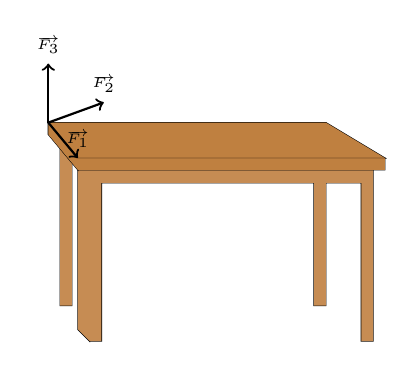
\begin{tikzpicture}[scale=1.5]
			%------------Bàn
			\def\O{
				%---chân bàn
				(.4,.05)--(.5,.05)--(.5,-1.3)--(.4,-1.4)--cycle
				(.65,.45)--(.65,-1.1)--(.55,-1.1)--(.55,.45)--cycle
				(-2,.05)--(-2,-1.4)--(-1.9,-1.4)--(-1.9,-.06)--(-1.6,-.06)--(-1.6,-1.1)--(-1.5,-1.1)--(-1.5,-.06)--(.3,-.06)--(.3,-1.4)--(.4,-1.4)--(.4,-.06)--(.4,.05)--cycle
				;}
			\draw[rotate=180,yscale=-1] \O;
			\fill[brown!90,rotate=180,yscale=-1] \O;
			%--mặt bàn
			\def\Z{
				(.5,.15)--(.75,.45)--(-1.6,.45)--(-2.1,.15)--cycle
				(.5,.15)--(.5,.05)--(-2.1,.05)--(-2.1,.15)--cycle
				(.5,.15)--(.5,.05)--(.75,.35)--(.75,.45)--cycle
				;}
			\draw[rotate=180,yscale=-1] \Z;
			\fill[brown,rotate=180,yscale=-1] \Z;
			\draw[ultra thin,rotate=180,yscale=-1] (-2.1,.15)--(.5,.15)--(.75,.45);
			%---------------Véc-tơ
			\draw[->,thick] (-0.75,0.45)--(-.5,.15)node[above]{\tiny $\overrightarrow{F_1}$};
			\draw[->,thick] (-0.75,0.45)--++(20:0.5)node[above]{\tiny $\overrightarrow{F_2}$};
			\draw[->,thick] (-0.75,0.45)--++(90:0.5)node[above]{\tiny $\overrightarrow{F_3}$};
		\end{tikzpicture}
	\end{center}
	\loigiai{
		Gọi $\overrightarrow{F}$ là hợp lực của ba lực trên, ta có $\overrightarrow{F}=\overrightarrow{F}_1+\overrightarrow{F}_2+\overrightarrow{F}_3$.\\
		Khi đó vì $\overrightarrow{F}_3$ vuông góc hai lực $\overrightarrow{F}_1$, $\overrightarrow{F}_2$ nên ta có
		\allowdisplaybreaks
		\begin{align*}
			\left|\overrightarrow{F}\right|^2=\left (\overrightarrow{F}_1+\overrightarrow{F}_2+\overrightarrow{F}_3\right)^2&=\left|\overrightarrow{F}_1\right|^2+\left|\overrightarrow{F}_2\right|^2+\left|\overrightarrow{F}_3\right|^2+2\overrightarrow{F}_1\overrightarrow{F}_2+2\overrightarrow{F}_2\overrightarrow{F}_3+2\overrightarrow{F}_3\overrightarrow{F}_1\\
			&=9^2+4^2+7^2+2\cdot 9 \cdot 4 \cdot \cos 100^\circ\\
			&=146+72\cos 100^\circ.
		\end{align*}
		Vậy $\left|\overrightarrow{F}\right|=\sqrt{146+72\cos 100^\circ}\approx12$ N.
	}
\end{ex}

% #100 | Archive/SP_SauLuoi_2024-2025/SP_HKI/2-TN-DS-TLN-THPT-DinhTienHoang-NinhBinh-HKI-NH24-25.tex | mã gốc 2H2V2-6
\begin{ex}%[2H2V2-6]%[Dự án đề kiểm tra Toán 12 CHKI NH24-25- Nguyễn Trần Anh Tuấn]%[THPT Đinh Tiên Hoàng - Tỉnh Ninh Bình]
	Ba chiếc máy bay không người lái cùng bay lên tại một địa điểm. Sau một thời gian bay, chiếc máy bay thứ nhất cách điểm xuất phát về phía Đông $40$ km và về phía Nam $60$ km, đồng thời cách mặt đất $3$ km. Chiếc máy bay thứ hai cách điểm xuất phát về phía Bắc $90$ km và về phía Tây $50$ km, đồng thời cách mặt đất $6$ km. Chiếc máy bay thứ ba đang trong quá trình bay thì đột ngột mất tín hiệu, biết rằng lần cuối (trước khi mất tín hiệu) máy bay thứ nhất xác định được khoảng cách giữa máy bay thứ nhất và máy bay thứ ba là $2\sqrt{3\,401}$ km và máy bay thứ ba nằm giữa máy bay thứ nhất và thứ hai, đồng thời ba chiếc máy bay này thẳng hàng. Hãy xác định khoảng cách (\textit{tính bằng ki-lô-mét}) từ vị trí xuất phát đến lúc máy bay số ba mất tín hiệu.
	\loigiai{
		Chọn hệ trục tọa độ $Oxyz$, với gốc đặt tại điểm xuất phát của ba chiếc máy bay, trục $Ox$ hướng về phía Bắc, trục $Oy$ hướng về phía Tây, trục $Oz$ hướng thẳng đứng lên trời, đơn vị đo lấy theo ki-lô-mét (xem hình vẽ).
		\begin{center}
			\begin{tikzpicture}[line join=round,font=\footnotesize,line cap=round,>=stealth,scale=0.8]
				\draw[->] (0,0)--(4.1,0) node[below left] {$y$};
				\draw[->] (0,0)--(0,4.1) node[below left] {$z$};
				\draw[->] (0,0)--(-3.1,-2.6) node[above left] {$x$};
				\draw (0,0) node [below right] {$O$};
				\draw (4.1,0) node [right] {Tây};
				\draw (-3.1,-2.6) node [below] {Bắc};
				\begin{scope}
					\clip (-4,-4) rectangle (4,4);
					\draw[dashed] (3,0)	--(1.4,-1.5)--(-1.7,-1.5);
					\draw[dashed] (1.4,-1.5)--(1.4,2)--(0,3.2);
				\end{scope}
				\fill[black] (1.4,2) circle (3pt);
			\end{tikzpicture}
		\end{center}
		Chiếc máy bay thứ nhất có tọa độ $A(-60;-40;3)$.\\
		Chiếc máy bay thứ hai có tọa độ $B(90;50;6)$.\\
		Gọi tọa độ của máy bay thứ ba lúc mất tín hiệu là $C(a;b;c)$.\\
		Ta có $\overrightarrow{AB}=(150;90;3)$; $\overrightarrow{AC}=(a+60;b+40;c-3)$.\\
		Do ba máy bay thẳng hàng và $C$ nằm giữa $A$, $B$ nên $\overrightarrow{AB}$ và $\overrightarrow{AC}$ cùng hướng.\\
		Ta có $\dfrac{a+60}{150}=\dfrac{b+40}{90}=\dfrac{c-3}{3}=t>0\Rightarrow \heva{&a+60=150t\\&b+40=90t\\&c-3=3t.}$
		\allowdisplaybreaks
		\begin{align*}
			&A C=\sqrt{(a+60)^2+(b+40)^2+(c-3)^2}=2 \sqrt{3\,401}\\
			\Leftrightarrow &\sqrt{(150 t)^2+(90 t)^2+(3 t)^2}=2 \sqrt{3\,401} \\
			\Leftrightarrow &30\,609 t^2=4 \cdot 3\,401\\
			\Leftrightarrow & t^2=\dfrac{4}{9} \\
			\Rightarrow &t=\dfrac{2}{3} \text{ (vì $t>0$)}.
		\end{align*}
		Suy ra $a=40$, $b=20$, $c=5$.\\
		Khoảng cách từ vị trí xuất phát đến lúc máy bay số ba mất tín hiệu là $\sqrt{a^2+b^2+c^2}=45$ km.
		
	}
\end{ex}

% #226 | Archive/SP_SauLuoi_2024-2025/SP_GHKI/2-TL-TN-DS-THPT-PhanChuTrinh-Binhthuan-GHKI-NH24-25.tex | mã gốc 2H2V1-4
\begin{ex}%[2H2V1-4]%[Dự án đề kiểm tra Toán 12 GHKI NH24-25- Hieu Phan]%[THPT Phan Chu Trinh- Bình Thuận]
    Có ba lực $\overrightarrow{F_1}$, $\overrightarrow{F_2}$, $\overrightarrow{F_3}$ cùng tác động vào một vật. Biết $\overrightarrow{F_1}$ và $\overrightarrow{F_2}$ hợp với nhau một góc $120^\circ$ và có độ lớn lần lượt là $15$ N, $20$ N. Lực $\overrightarrow{F_3}$ vuông góc với mặt phẳng tạo bởi hai lực $\overrightarrow{F_1}$, $\overrightarrow{F_2}$ và có độ lớn $10\sqrt{3}$ N. Hợp lực của ba lực $\overrightarrow{F_1}$, $\overrightarrow{F_2}$, $\overrightarrow{F_3}$ có độ lớn bằng bao nhiêu?
    \loigiai{\immini
        {
            Giả sử ba lực $\overrightarrow{F_1}$, $\overrightarrow{F_2}$, $\overrightarrow{F_3}$ cùng tác động vào một vật đặt tại điểm $A$.\\
        Vẽ $\overrightarrow{AB}=\overrightarrow{F_1},\overrightarrow{AD}=\overrightarrow{F_2},\overrightarrow{AE}=\overrightarrow{F_3}$.\\
        Khi đó \begin{eqnarray*}
            \overrightarrow{F_1}+\overrightarrow{F_2}+\overrightarrow{F_3}&=&\left(\overrightarrow{AB}+\overrightarrow{AD}\right)+\overrightarrow{AE}\\
            &=&\overrightarrow{AC}+\overrightarrow{AE}=\overrightarrow{AH}.
        \end{eqnarray*}
        Ta có \begin{eqnarray*}
            AC^2&=&AB^2+BC^2-2AB\cdot BC\cdot \cos 60^0\\
            &=&15^2+20^2-2\cdot15\cdot 20\cdot \dfrac{1}{2}=325.
        \end{eqnarray*}
        }
        {
            	\begin{tikzpicture}[scale=0.9, font=\footnotesize, line join=round, line cap=round]
                %---------------------------
                \foreach \x\y\t in {0/0/A, -2/-1.3/B, 4/0/D,0/3/E}
                \coordinate (\t) at (\x,\y);
                \coordinate (C) at ($(D)+(B)$);
                \coordinate (H) at ($(E)+(C)$);
                \coordinate (x) at (intersection of D--A and H--C);
                \path (x)--(A)node[pos=0.5,above]{$\overrightarrow{F_2}$};
                \path (A)--(B)node[pos=0.5,above left]{$\overrightarrow{F_1}$};
                \path (A)--(E)node[pos=0.5,left]{$\overrightarrow{F_3}$};
                \path (A) pic[draw,angle radius=6]{angle=B--A--D}node[shift={(-85:10pt)}]{$120^{\circ}$};
                \foreach \a\b in {A/B, x/D,A/C,A/E,A/H}
                \draw[-stealth] (\a)--(\b);
                \draw (B)--(C)--(D) (E)--(H)--(C);
                \draw[dashed] (A)--(x);
                \foreach \t\g in {A/170, D/90, B/150,E/90,C/-80,H/45}
                \draw[fill=black] (\t)circle(0.6pt) +(\g:8pt)node{$\t$};
            \end{tikzpicture}
        }
     \noindent Suy ra $ AH=\sqrt{AC^2+CH^2}=\sqrt{325+\left(10\sqrt{3}\right)^2}=25 $.\\
    Vậy hợp lực của ba lực $\overrightarrow{F_1},\overrightarrow{F_2},\overrightarrow{F_3}$ có độ lớn bằng $25$ N.
        } 
\end{ex}

% #499 | Archive/2024/San pham - To Latex Strong - Tex hoa Lop 12 moi - Dot 2 (Chuong 1 + 2 + 3)/San pham - To Latex Strong - Tex hoa Lop 12 moi - Dot 2 (Chuong 1 + 2 + 3)/Data/Chuong 2/Ket noi tri thuc/To 21 - Dot 16 - Chuong 2 - On tap chuong - KNTT - De 3.tex | mã gốc 2H2C2-6
\begin{ex}%[2H2C2-6]%[Tổ 21 - Đợt 16 - Chương 2 - Ôn tập chương - Đề 3 - KNTT]%[Tex hóa: Lê Thị Thúy Hằng]
	\immini{
	Một chiếc đèn trang trí hình tròn được treo song song với mặt phẳng trần nhà nằm ngang bởi ba sợi dây không giãn $ OA,\,OB,\,OC$ đôi một vuông góc (như hình vẽ dưới đây). Biết lực căng dây tương ứng trên mỗi dây $OA$, $OB$, $OC$ lần lượt là $\overrightarrow{F_1}$, $\overrightarrow{F_2}$, $\overrightarrow{F_3}$ thỏa mãn $\left|\overrightarrow{F_1}\right|=\left|\overrightarrow{F_2}\right|=\left|\overrightarrow{F_3}\right|=16$(N). Tính trọng lượng (đơn vị: N) của chiếc đèn đó. (Làm tròn kết quả đến hàng phần chục).
	}{
	\begin{tikzpicture}[scale=.5, font=\footnotesize, line join=round, line cap=round, >=stealth,transform shape]
		\def\r{3}
		\def\gA{-160}
		\def\gB{130}
		\path
		(0:0) coordinate (I)
		(0:\r) coordinate (C) 
		(180:\r) coordinate (D)
		(-90:\r/3) coordinate (M)
		(C) arc (0:\gA:{\r} and {\r/3}) coordinate (A)
		(C) arc (0:\gB:{\r} and {\r/3}) coordinate (B)
		($(O)!0.5!(A)$) coordinate (A1)
		($(O)!0.7!(B)$) coordinate (B1)
		($(O)!0.4!(C)$) coordinate (C1)
		(I)++(90:2.6*\r) coordinate (O)
		\foreach \x in {I,C,D,M}{(\x)++(-90:0.05*\r) coordinate (\x')}
		(I')++(-90:1.6*\r) coordinate (P)
		(O)++(0:0.6*\r) coordinate (O1)
		(O)++(180:0.6*\r) coordinate (O2)
		;
		\fill[blue!20!white] (C') arc (0:-180:{\r} and {\r/3});
		\draw[line width=1pt] 
		(I') ellipse ({\r} and {\r/3})
		;
		\fill[blue!10!white] (I) ellipse ({\r} and {\r/3});
		\fill[red] 
		(I) circle(2pt)
		;
		\draw[line width=0.8pt] (I) ellipse ({\r} and {\r/3});
		\draw[line width=1pt] (A)--(O)--(B) (O)--(C);
		\draw[line width=1pt, ->] (O) -- (A1) node[left] {$\vec{F_1}$};
		\draw[line width=1pt, ->] (O) -- (B1) node[right] {$\vec{F_2}$};
		\draw[line width=1pt, ->] (O) -- (C1) node[right] {$\vec{F_3}$};
		\draw[line width=1pt, ->] (M') -- (P) node[midway,right] {$\vec{P}$};
		\draw[dashed] (C)--(I)--(M');
		\draw[line width=2pt] (O1)--(O2);
		\draw 
		(O) node[below right]{$O$}
		(A) node[above right]{$A$}
		(B) node[above right]{$B$}
		(C) node[right]{$C$}
		;
	\end{tikzpicture}
	}
	%\end{center}
	\loigiai{
		%FB tác giả: Phạm Thị Thu Hà
	\immini{
		Ta có: $P=\left|\overrightarrow{F_1}+\overrightarrow{F_2}+\overrightarrow{F_3}\right|=\left|\overrightarrow{OA}+\overrightarrow{OB}+\overrightarrow{OC}\right|$ .\\
		Vẽ hình vuông $ OAEB$, ta có $\overrightarrow{OA}+\overrightarrow{OB}=\overrightarrow{OE}$ . (Quy tắc hình bình hành)\\
		Vẽ hình chữ nhật $ OCFE$, ta có $\overrightarrow{OC}+\overrightarrow{OE}=\overrightarrow{OF}$ . (Quy tắc hình bình hành)\\
		Suy ra: $P=\left|\overrightarrow{OF}\right|=OF$ .\\
		Xét hình vuông $ OAEB$, cạnh $ 16$, có đường chéo $ OE=16\sqrt{2}$.\\
		Xét tam giác vuông $ OEF$, vuông tại $E$, ta có \\ $OF = \sqrt{OE^2+EF^2}=\sqrt{\left(16\sqrt{2}\right)^2+16^2}=16\sqrt{3}\approx 27,7$.\\
		Vậy $ P\approx 27,7$(N).
	}{
		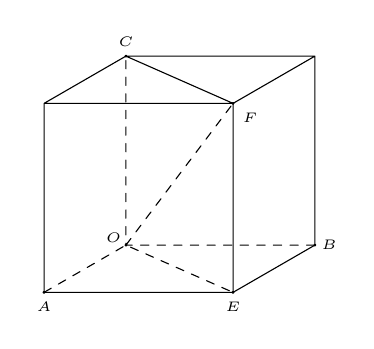
\begin{tikzpicture}[scale=.6, font=\tiny, line join=round, line cap=round, >=stealth]
			\def\a{4}
			\path 
			(0:0) coordinate (A)
			(0:\a) coordinate (E)
			++(30:\a/2) coordinate (B)
			++(180:\a) coordinate (O)
			\foreach \x in {A,E,B,O}{(\x)++(90:\a) coordinate (\x')}
			;
			\draw (A)--(E)--(E')--(A')--cycle 
			(A')--(O')--(E')--(B')--(O')
			(E)--(B)--(B')
			;
			\draw[dashed] (A)--(O)--(E) (O)--(E') (B)--(O)--(O');
			\foreach \x/\g in {A/-90,E/-90,B/0,O/150}
			\draw[fill=black] (\x) circle (0.02)+ (\g:0.3) node{$\x$};
			\draw[fill=black] (O') circle (0.02) node[above]{$C$};
			\draw[fill=black] (E') circle (0.02) node[below right]{$F$};
		\end{tikzpicture}
	}
	}
\end{ex}

% #600 | Archive/2024/San pham - To Latex Strong - Tex hoa Lop 12 moi - Dot 2 (Chuong 1 + 2 + 3)/San pham - To Latex Strong - Tex hoa Lop 12 moi - Dot 2 (Chuong 1 + 2 + 3)/Data/Chuong 2/Chan troi sang tao/To 4 - Dot 17 - Chuong 2 - On tap chuong - CTST - De 2.tex | mã gốc 2H2H2-4
\begin{ex}%[2H2H2-4]%[Tổ 4 - Đợt 17 - Chương 2 - Đề 2 - CTST]%[Huỳnh Thanh Chí]
	Một thiết bị thăm dò đáy biển được đẩy bởi một lực $\overrightarrow{f}=(5; 2;-7)$ (đơn vị: N) giúp thiết bị thực hiện độ dời $\overrightarrow{a}=(10; 20;-20)$ (đơn vị: m). Gọi $A$ là công sinh bởi lực $\overrightarrow{f}$. Tính $A$.
	\loigiai{Công sinh bởi lực $\overrightarrow{f}$ khi thực hiện độ dời $\overrightarrow{a}$ là
		$A=\overrightarrow{f} \cdot \overrightarrow{a}=5\cdot 10+2\cdot 10+(-7)\cdot (-20)=210$ (N).
	}
\end{ex}

% #704 | Archive/2024/San pham - To Latex Strong - Tex hoa Lop 12 moi - Dot 2 (Chuong 1 + 2 + 3)/San pham - To Latex Strong - Tex hoa Lop 12 moi - Dot 2 (Chuong 1 + 2 + 3)/Data/Chuong 2/Canh dieu/To 9 - Dot 16 - Chuong 2 - On tap chuong - CD - De 1.tex | mã gốc 2H2C2-6
\begin{ex}%[2H2C2-6]
	Một chậu cây được đặt trên một giá đỡ có bốn chân với điểm đặt $S\left(0;0;30\right)$ và các điểm chạm mặt đất của bốn chân lần lượt là $A\left(30;0;0\right)$, $B\left(0;20;0\right)$, $C\left(-20;0;0\right)$, $D\left(0;-20;0\right)$ (đơn vị cm). Cho biết trọng lực tác dụng lên chậu cây có độ lớn $60$ N và được phân bố thành bốn lực $\overrightarrow{F_1}$, $\overrightarrow{F_2}$, $\overrightarrow{F_3}$, $\overrightarrow{F_4}$ có độ lớn bằng nhau như hình vẽ. Tính $\left|\overrightarrow{F_1}+2\overrightarrow{F_2}+3\overrightarrow{F_3}+4\overrightarrow{F_4}\right|$ (kết quả làm tròn đến hàng đơn vị)
\loigiai{
	\begin{center}
		\begin{tikzpicture}[declare function={a=2;b=4;h=4;},line join=round]
			\path (0,0) coordinate (A)
			(-145:a) coordinate (B)
			(b,0) coordinate (D)
			($ (B)!0.5!(D) $) coordinate (O)
			($(O)+(0,h) $) coordinate (S);
			\path ($(D)-(A)+(B)$) coordinate (C);
			\path ($(S)!0.4!(A)$) coordinate (A')
			($(S)!0.5!(B)$) coordinate (B')
			($(S)!0.5!(C)$) coordinate (C')
			($(S)!0.4!(D)$) coordinate (D');	
			
			\draw[dashed] (S)--(A)--(B) (A)--(D)--(B) (A)--(C) (S)--(O) (D')--(A')--(B')--(D') (A')--(C');
			\draw (B)--(C)--(D) (B)--(S)  (D)--(S)--(C) (B')--(C')--(D');
			\draw[->,red,thick] (S)--(B');
			\draw[->,red,thick] (S)--(C');
			\draw[->,red,thick] (S)--(D');
			\draw[->,red,thick,dashed] (S)--(A');
			\path (S)--(D')node[pos=0.5,sloped,black,above,scale=0.6]{$\overrightarrow{F_4}$}
			(S)--(C')node[pos=0.5,sloped,black,above,scale=0.6]{$\overrightarrow{F_3}$}
			(S)--(A')node[pos=0.7,sloped,black,below,scale=0.6]{$\overrightarrow{F_1}$}
			(B')--(S)node[pos=0.5,sloped,black,above,scale=0.6]{$\overrightarrow{F_2}$}
			;
			\path (intersection of A'--C' and B'--D') coordinate (O');
			
			\foreach \t/\g in {A/150,B/-90,C/-90,D/0,S/90,O/-90,A'/150,B'/150,C'/0,D'/60,O'/0}{
				\draw[fill=white] (\t) circle (1pt) node[shift={(\g:6pt)},font=\scriptsize]{$ \t $};
			}
		\end{tikzpicture}
	\end{center}
Tứ giác $ABCD$ có hai đường chéo bằng nhau và vuông góc với nhau tại trung điểm của mỗi đường nên là hình vuông.\\
Ta có
\begin{itemize}
	\item $\overrightarrow{SA}=\left(30;0;-30\right)$.
	\item $\overrightarrow{SB}=\left(0;20;-20\right)$.
	\item $\overrightarrow{SC}=\left(-20;0;-20\right)$,
	\item $\overrightarrow{SD}=\left(0;-20;-20\right)$
\end{itemize} 
$\Rightarrow SA=SB=SC=SD=30\sqrt{2}$. Do đó $S.ABCD$ là hình chóp tứ giác đều.\\
Các véc-tơ $\overrightarrow{F_1}$, $\overrightarrow{F_2}$, $\overrightarrow{F_3}$, $\overrightarrow{F_4}$ có điểm đầu tại $S$ và điểm cuối lần lượt là $A'$, $B'$, $C'$, $D'$.\\
Ta có $SA'=SB'=SC'=SD' $ nên $S.A'B'C'D'$ cũng là hình chóp tứ giác đều.\\
Gọi $\overrightarrow{F}$ là trọng lực tác dụng lên chậu cây và $O'$ là tâm của hình vuông $A'B'C'D'$. Ta có 
	\[\overrightarrow{F}=\overrightarrow{F_1}+\overrightarrow{F_2}+\overrightarrow{F_3}+\overrightarrow{F_4}=\overrightarrow{SA'}+\overrightarrow{SB'}+\overrightarrow{SC'}+\overrightarrow{SD'}=4\overrightarrow{SO'}.\]
Mặt khác
		\[\left|\overrightarrow{F}\right|=60\Rightarrow \left|\overrightarrow{SO'}\right|=SO=15.\]
		Do tam giác $SO'A'$ vuông cân nên $SA'=SO'\sqrt{2}=15\sqrt{2}=\dfrac{1}{2} SA$\\
		Suy ra $\overrightarrow{F_1}=\overrightarrow{SA'}=\dfrac{1}{2} \overrightarrow{SA}=\left(15;0;-15\right)$.\\
		Chứng minh tương tự ta cũng có
		\[\overrightarrow{F_2}=\dfrac{1}{2} \overrightarrow{SB}=\left(0;15;-15\right),\overrightarrow{F_3}=\dfrac{1}{2} \overrightarrow{SC}=\left(-15;0;-15\right),\overrightarrow{F_4}=\dfrac{1}{2} \overrightarrow{SD}=\left(0;-15;-15\right).
		\]
		Suy ra $\overrightarrow{F_1}+2\overrightarrow{F_2}+3\overrightarrow{F_3}+4\overrightarrow{F_4}=\left(-30;-30;-150\right)$.\\
		Vậy $ \left|\overrightarrow{F_1}+2\overrightarrow{F_2}+3\overrightarrow{F_3}+4\overrightarrow{F_4}\right|=90\sqrt{3} \approx 156$.
	}
\end{ex}

% #731 | Archive/2024/San pham - To Latex Strong - Tex hoa Lop 12 moi - Dot 2 (Chuong 1 + 2 + 3)/San pham - To Latex Strong - Tex hoa Lop 12 moi - Dot 2 (Chuong 1 + 2 + 3)/Data/Chuong 2/Canh dieu/To 8 - Dot 16 - Chuong 2 - Bai 3 - CD - De 1.tex | mã gốc 2H2H2-6
\begin{ex}%[2H2H2-6]%[To8-Dot16-Chuong2-Bai2-CD-De1]%[Lê Quân]
Một em nhỏ cân nặng $20kg$ trượt trên cầu trượt dài 3m. Biết rằng cầu trượt có góc nghiêng so với phương nằm ngang là $30^\circ$. Cho biết công A(J) sinh bởi một lực $\overrightarrow F $ có độ dịch chuyển $\overrightarrow d $ được tính bởi công thức $A=\overrightarrow{F}\cdot\overrightarrow d $. Hãy tính công sinh bởi trọng lực $\overrightarrow P $ khi em nhỏ trượt hết chiều dài cầu trượt biết gia tốc rơi tự do $g=9{,}8\,\mathrm{m}/{s^2}$.
\begin{center}
\tikzset{
		ex_markstyle/.style={},
		ex_mark/.style  n args={1}{decoration={ markings, %
				mark= at position 0.5 with
				with{
					\ifnum#1=1
					\draw[ex_markstyle] (0pt,-2pt) -- (0pt,2pt);
					\fi
					\ifnum#1=2
					\draw[ex_markstyle] (-1pt,-2pt) -- (-1pt,2pt);
					\draw[ex_markstyle] (1pt,-2pt) -- (1pt,2pt);
					\fi
					\ifnum#1=3
					\draw[ex_markstyle] (-2pt,-2pt) -- (-2pt,2pt);
					\draw[ex_markstyle] (0pt,-2pt) -- (0pt,2pt);
					\draw[ex_markstyle] (2pt,-2pt) -- (2pt,2pt);
					\fi
					\ifnum#1=4
					\draw[ex_markstyle] (-1pt,-1pt) -- (1pt,1pt);
					\draw[ex_markstyle] (-1pt,1pt) -- (1pt,-1pt);
					\fi
			} },
			pic actions/.append code=\tikzset{postaction=decorate}},
	}
	\definecolor{cambridgeblue}{rgb}{0.64, 0.76, 0.68}
	\definecolor{camel}{rgb}{0.76, 0.6, 0.42}%màu cầu tuột 1 
	\definecolor{cadetblue}{rgb}{0.37, 0.62, 0.63}%màu cầu tuột 2  
	\definecolor{canaryyellow}{rgb}{1.0, 0.94, 0.0}%Màu giày bé gái 
	\definecolor{byzantine}{rgb}{0.74, 0.2, 0.64}%Màu quần bé gái 
	\definecolor{carrotorange}{rgb}{0.93, 0.57, 0.13}%Màu áo bé gái 
	\definecolor{cerulean}{rgb}{0.0, 0.48, 0.65}%màu giày 
	\definecolor{caribbeangreen}{rgb}{0.0, 0.8, 0.6}%màu áo 
	\definecolor{ceruleanblue}{rgb}{0.16, 0.32, 0.75}%màu quần 
	\definecolor{crimsonglory}{rgb}{0.75, 0.0, 0.2}%màu môi
	\definecolor{darkjunglegreen}{rgb}{0.1, 0.14, 0.13}%màu tóc 
	\definecolor{apricot}{rgb}{0.98, 0.81, 0.69}%màu da
	\begin{tikzpicture}[line join=round, line cap=round,scale=.6,transform shape]
		\clip (-11,-10) rectangle (25,4);
		\tikzset{be_trai/.pic={ 
				\def\T{ 
					(1.5,2.8)
					..controls +(-125:.1) and +(40:.2) ..(1.3,2.6)
					..controls +(75:.1) and +(-100:.1) ..(1.35,2.75)
					..controls +(-125:.1) and +(40:.2) ..(.9,2.5)
					..controls +(65:.1) and +(-110:.2) ..(1,2.7)
					..controls +(-125:.1) and +(40:.2) ..(.65,2.4)
					..controls +(-110:.1) and +(80:.1) ..(.6,2.1)%vành tai 
					..controls +(120:.1) and +(60:.1) ..(.3,2.15)%đỉnh tai 
					..controls +(130:.4) and +(-120:.4) ..(.2,3)
					..controls +(60:.8) and +(85:.9) ..(1.7,2.55)
					..controls +(110:.2) and +(-35:.2) ..cycle 
					;
				}
				\fill[darkjunglegreen] \T;
				\draw[black]\T;
				%----------------------------------------
				%Cổ 
				\def\C{ 
					(.7,1.8)--(.68,1.6)
					..controls +(-65:.3) and +(-120:.3) ..(1.2,1.5)--
					(1.2,1.7)--cycle
					;
				}
				\fill[apricot!60] \C;
				\draw[black]\C;
				%---------------------------
				%Mặt
				\def\M{ 
					(1.5,2.8)
					..controls +(-125:.1) and +(40:.2) ..(1.3,2.6)
					..controls +(75:.1) and +(-100:.1) ..(1.35,2.75)
					..controls +(-125:.1) and +(40:.2) ..(.9,2.5)
					..controls +(65:.1) and +(-110:.2) ..(1,2.7)
					..controls +(-125:.1) and +(40:.2) ..(.65,2.4)
					..controls +(-110:.1) and +(80:.1) ..(.6,2.1)%vành tai 
					..controls +(120:.1) and +(60:.1) ..(.3,2.15)%đỉnh tai 
					..controls +(-120:.2) and +(-170:.2) ..(.6,1.9)
					..controls +(-55:.4) and +(-95:.7) ..(1.65,2.2)
					..controls +(-5:.1) and +(20:.15) ..(1.63,2.4)
					..controls +(85:.2) and +(-20:.15) ..cycle 
					;
				}
				\fill[apricot!60] \M;
				\draw[black]\M;
				
				%mày trái 
				\draw[black,line width=.25mm] (1.35,2.52)
				..controls +(35:.1) and +(135:.1) ..(1.55,2.5)
				;
				%mắt trái 
				\draw[black] (1.35,2.3)
				..controls +(65:.1) and +(115:.1) ..(1.55,2.35)
				..controls +(-110:.12) and +(-40:.1) ..cycle;
				%mắt phải 
				\draw[black] (.85,2.2)
				..controls +(65:.1) and +(115:.1) ..(1.1,2.25)
				..controls +(-110:.12) and +(-40:.1) ..cycle
				;
				%mày phải 
				\draw[black,line width=.25mm]  (.8,2.35)
				..controls +(55:.1) and +(-165:.1) ..(1,2.5);
				%môi  
				\draw[black,fill=crimsonglory]  (1.1,1.95)
				..controls +(55:.1) and +(-165:.1) ..(1.4,2)
				..controls +(-115:.25) and +(-55:.1) ..cycle ;
				%con ngươi 
				\draw[xscale=.86,fill=black] (1.7,2.33) circle (.055);
				\draw[xscale=.86,fill=black] (1.15,2.22) circle (.06);
				
				%Quần 
				\def\Q{ 
					(.3,0)
					..controls +(-120:.1) and +(80:.2) ..(.25,-.35)
					..controls +(-100:.4) and +(150:.4) ..(1.55,-1.45)
					..controls +(70:.2) and +(170:.2) ..(1.8,-.9)%giữa quần 
					--(2,-1.05)
					..controls +(50:.1) and +(150:.1) ..(2.35,-.8)
					..controls +(150:.1) and +(-40:.15) ..(1.75,-.15)
					..controls +(150:.1) and +(-40:.15) ..cycle
					;
				}
				\fill[ceruleanblue] \Q;
				\draw[black]\Q;
				\draw (1.8,-.9)..controls +(150:.1) and +(-40:.15) .. (1.25,-.4);
				
				%Chân  
				\def\C{ 
					(1.55,-1.45)
					..controls +(70:.2) and +(170:.2) ..(1.8,-.9)%giữa quần 
					--(2,-1.05)
					..controls +(50:.1) and +(150:.1) ..(2.35,-.8)
					..controls +(-50:.1) and +(140:.15) ..(2.85,-1.4)
					..controls +(-150:.1) and +(70:.15) ..(2.65,-1.67)%giữa chân 
					..controls +(-150:.1) and +(70:.15) ..(2.45,-2.05)
					..controls +(150:.1) and +(-60:.15) ..cycle 
					;
				}
				\fill[apricot!80] \C;
				\draw[black]\C;
				\draw (2.65,-1.67)%giữa chân 
				..controls +(140:.1) and +(-60:.15) ..(2,-1.05);
				
				%Giày   
				\def\G2{ 
					(3.25,-1.4)
					..controls +(-150:.1) and +(70:.15) ..(3.05,-1.67)%giữa chân 
					..controls +(-150:.1) and +(70:.15) ..(2.85,-2.05)
					..controls +(-110:.6) and +(-100:.8) ..(3.6,-2.05)
					..controls +(60:.6) and +(30:.2) ..cycle
					;
				}
				\fill[cerulean] \G2;
				\draw[black]\G2;
				
				\draw (3.6,-1.5)%giữa chân 
				..controls +(150:.1) and +(70:.15) ..(3.3,-1.7);
				\draw (3.55,-1.45)
				..controls +(150:.1) and +(70:.15) ..(3.2,-1.7);
				
				\def\G1{ 
					(2.85,-1.4)
					..controls +(-150:.1) and +(70:.15) ..(2.65,-1.67)%giữa chân 
					..controls +(-150:.1) and +(70:.15) ..(2.45,-2.05)
					..controls +(-110:.6) and +(-100:.8) ..(3.2,-2.05)
					..controls +(60:.6) and +(30:.2) ..cycle
					;
				}
				\fill[cerulean] \G1;
				\draw[black]\G1;
				\draw (3.2,-1.5)%giữa chân 
				..controls +(150:.1) and +(70:.15) ..(2.9,-1.7);
				\draw (3.15,-1.45)
				..controls +(150:.1) and +(70:.15) ..(2.8,-1.7);
				
				%Tay trái 
				\def\T2{ 
					(1.92,.6)
					..controls +(-60:.2) and +(160:.2) ..(2.5,-.15)
					..controls +(-40:.1) and +(140:.1) ..(2.95,-.4)
					..controls +(-40:.02) and +(-40:.1) ..(2.82,-.4)
					..controls +(-30:.3) and +(-40:.3) ..(2.72,-.4)
					..controls +(-30:.4) and +(-40:.5) ..(2.6,-.4)
					..controls +(-40:.4) and +(-50:.5) ..(2.52,-.45)
					..controls +(130:.1) and +(70:.2) ..(2.2,-.6)
					..controls +(-150:.3) and +(-55:.3) ..(2.1,-.2)
					..controls +(150:.3) and +(-55:.2) ..(1.4,.6)--cycle
					;
				}
				\fill[apricot!60] \T2;
				\draw[black]\T2;
				
				%Áo 
				\def\A{ 
					(.68,1.6)
					..controls +(-65:.3) and +(-120:.3) ..(1.2,1.5)--(1.2,1.6)
					..controls +(-20:.7) and +(120:.6) ..(2,.7)
					..controls +(-120:.3) and +(20:.2) ..(1.65,.5)
					..controls +(-90:.3) and +(120:.2) ..(1.75,-.15)
					..controls +(-150:.3) and +(30:.2) ..(.45,-.35)
					..controls +(140:.2) and +(-70:.2) ..(.3,0)
					..controls +(-120:.1) and +(80:.2) ..(.25,-.35)--(.2,-.32)
					..controls +(90:.1) and +(-100:.2) ..(.22,.35)--(-.3,.7)
					..controls +(70:.3) and +(-175:.3) ..cycle
					;
				}
				\fill[caribbeangreen] \A;
				\draw[black]\A;
				
				%Tay phải
				\def\T{ 
					(.22,.35)..controls +(-145:.4) and +(-110:.5) ..(-.3,.7)
					..controls +(45:.2) and +(-160:.2) ..(.45,.8)
					..controls +(75:.2) and +(178:.4) ..(.8,1.15)
					..controls +(-2:0) and +(60:0) ..(.85,1.1)
					..controls +(-30:.04) and +(60:.02) ..(.88,1)
					..controls +(2:0) and +(30:.05) ..(.9,.9)
					..controls +(2:0) and +(30:.05) ..(.9,.8)
					..controls +(175:0) and +(-5:.05) ..(.75,.78)
					..controls +(-95:.2) and +(0:.1) ..(.5,.5)
					..controls +(-160:.2) and +(35:.1) ..cycle
					;
				}
				\fill[apricot!60] \T;
				\draw[black]\T;
				\draw (.85,1.1)
				..controls +(-175:.1) and +(20:.1) ..(.65,1.08);
				\draw (.88,1)
				..controls +(-175:.1) and +(20:.1) ..(.7,.98);
				
				\draw (.9,.9)
				..controls +(-175:.1) and +(20:.1) ..(.75,.88);
		}}
		
		
	
		
		
		\tikzset{cau_truot_1/.pic={ 
				%====================Dài 
				\draw[line width=1.5mm,shift={(1,.6)}] (-6,1.7)--(-6,2.8)
				..controls +(90:.3) and +(180:.3) ..(-5,3)
				..controls +(0:.3) and +(90:.3) ..(-4,2.8)--(-4,1.7)
				;
				\draw[line width=1.5mm] (-6,1.7)--(-6,2.8)
				..controls +(90:.3) and +(180:.3) ..(-5,3)
				..controls +(0:.3) and +(90:.3) ..(-4,2.8)--(-4,1.7)
				;
				\def\D{ 
					(-6,1.7)
					..controls +(-180:.6) and +(180:.6) ..(-6,.7)--(-4,.7)--(8.8,-6.9)--(12.5,-6.9)..controls +(0:.6) and +(-0:.6) ..(12.5,-5.85)--(9.5,-5.85)--(-3.2,1.7)--cycle 
					;
				}
				\fill[shift={(1,.6)},cadetblue] \D;
				\draw[shift={(1,.6)},black]\D;
				%\fill[cadetblue] \D;
				\draw[black]\D;
				
				\draw[fill=cambridgeblue] (-3.7,1.8) circle (.2);
				\draw[fill=cambridgeblue] (-2.9,1.8) circle (.2);
				\draw[fill=cambridgeblue] (-4.5,1.8) circle (.2);
				
				
		}}
		\tikzset{cau_truot_2/.pic={ 
				\def\T{ 
					(-6.35,1.1)
					..controls +(80:.5) and +(60:.4) ..(-5.7,1)--(-8.6,-6.8)
					..controls +(-120:.5) and +(-100:.4) ..(-9.35,-6.7)--cycle
					;
				}
				
				%--------------------------
				\def\Th{ 
					(-4.75,-.3)
					..controls +(-30:.1) and +(50:.1) ..(-4.7,-.6)--(-6.5,-.8)
					..controls +(150:.1) and +(-150:.1) ..(-6.5,-.5)--cycle 
					;
				}
				
				\fill[shift={(1.8,.3)},camel] \T;
				\draw[shift={(1.8,.3)},black]\T;
				
				\fill[camel] \Th;
				\draw[black]\Th;
				\fill[shift={(-.5,-1.3)},camel]\Th;
				\fill[shift={(-1,-2.5)},camel]\Th;
				\fill[shift={(-1.4,-3.7)},camel]\Th;
				\fill[shift={(-1.9,-4.9)},camel]\Th;
				
				\draw[shift={(-.5,-1.3)},black]\Th;
				\draw[shift={(-1,-2.5)},black]\Th;
				\draw[shift={(-1.4,-3.7)},black]\Th;
				\draw[shift={(-1.9,-4.9)},black]\Th;
				
				\fill[camel] \T;
				\draw[black]\T;
				%====================Dài 
				\draw[line width=1.5mm,shift={(1,.6)}] (-6,1.7)--(-6,2.8)
				..controls +(90:.3) and +(180:.3) ..(-5,3)
				..controls +(0:.3) and +(90:.3) ..(-4,2.8)--(-4,1.7)
				;
				\draw[line width=1.5mm] (-6,1.7)--(-6,2.8)
				..controls +(90:.3) and +(180:.3) ..(-5,3)
				..controls +(0:.3) and +(90:.3) ..(-4,2.8)--(-4,1.7)
				;
				\def\D{ 
					(-6,1.7)
					..controls +(-180:.6) and +(180:.6) ..(-6,.7)--(-4,.7)--(8.8,-6.9)--(12.5,-6.9)..controls +(0:.6) and +(-0:.6) ..(12.5,-5.85)--(9.5,-5.85)--(-3.2,1.7)--cycle 
					;
				}
				
				\fill[cadetblue] \D;
				\draw[black]\D;
				
				\fill[camel] \T;
				\draw[black]\T;
				\draw[fill=cambridgeblue] (-6,1.1) circle (.2);
				\draw[fill=cambridgeblue] (-5.2,1.1) circle (.2);
				\draw[fill=cambridgeblue] (-4.4,1.1) circle (.2);
				
				
		}}
		
		\path 
		%(0,0)pic[scale=1]{be_gai}
		(0,0)pic[scale=1]{cau_truot_1}
		(0,0)pic[scale=1]{be_trai}
		(0,0)pic[scale=1]{cau_truot_2}
		;
		
		\path 	(-3,1) coordinate (A)
		(-3,-6) coordinate (B)
		(9,-6) coordinate (C)
		;
		\node at (B) [left]{$B$};
		\node at (A) [left]{$A$};
		\node at (C) [below]{$D$};
		\node at (.8,-3.5) [below]{$\overrightarrow{P}$};
		\draw[dashed] (B)--(C)--(A)--cycle;
		\draw[line width=.7mm,red,->](.8,-2.2)--(.8,-3.5);
		\draw pic["$30^\circ$", draw=red,angle eccentricity=1.6, ex_mark=1,angle radius=.6cm, color=red]
		{angle=A--C--B};
		\draw pic[draw=black, angle radius=.5cm]
		{right angle=C--B--A};
	\end{tikzpicture}
\end{center}
\loigiai{
Ta có $\left|\overrightarrow P\right|=P=m\cdot g=20\cdot 9{,}8=196$ (N) và 
$\left|\overrightarrow d\right|=\left|\overrightarrow{AC}\right|=AC=3(\mathrm{m})$.\\
Cầu trượt có góc nghiêng so với phương nằm ngang là $\widehat{ACB}=30^\circ$ nên \[ \left(\overrightarrow P;\overrightarrow{d}\right)=\widehat{CAB}=60^\circ.\]
Công sinh bởi trọng lực $\overrightarrow P $ khi em nhỏ trượt hết chiều dài cầu trượt $3\,$ m là
\[A=\overrightarrow{P}\cdot \overrightarrow d=\left|\overrightarrow P\right|\cdot\left|\overrightarrow d\right|\cos \left(\overrightarrow P;\overrightarrow{d}\right)=196\cdot 3\cdot\cos{60^\circ}=294\,(\mathrm{J}).\]}
\end{ex}

% #1177 | Archive/2024/0. [LVH] BG - 12 New - 4in1-20240625T224301Z-001/0. [LVH] BG - 12 New - 4in1/2. [LVH] TEX SGK 12 NEW-20240418T074833Z-001/2. [LVH] TEX SGK 12 NEW/[LVH] SGK-12-KNTT/data/C2/12-SGK-KNTT-2-6.tex | mã gốc 2H2N1-1
\begin{bt}%[2H2N1-1]
Trong không gian, cho ba véc-tơ $\overrightarrow{a}$, $\overrightarrow{b}$, $\overrightarrow{c}$ phân biệt và đều khác $\overrightarrow{0}$. Những mệnh đề nào sau đây là đúng?
	\begin{enumerate}[a)]	
		\item Nếu $\overrightarrow{a}$ và $\overrightarrow{b}$ đều cùng hướng với $\overrightarrow{c}$ thì $\overrightarrow{a}$ và $\overrightarrow{b}$ cùng hướng.
	\item 	Nếu $\overrightarrow{a}$ và $\overrightarrow{b}$ đều ngược hướng với $\overrightarrow{c}$ thì $\overrightarrow{a}$ và $\overrightarrow{b}$ cùng hướng.
\item 		Nếu $\overrightarrow{a}$ và $\overrightarrow{b}$ đều cùng hướng với $\overrightarrow{c}$ thì $\overrightarrow{a}$ và $\overrightarrow{b}$ ngược hướng.
\item 		Nếu $\overrightarrow{a}$ và $\overrightarrow{b}$ đều ngược hướng với $\overrightarrow{c}$ thì $\overrightarrow{a}$ và $\overrightarrow{b}$ ngược hướng.
	\end{enumerate}
	\loigiai{
	\begin{enumerate}[a)]	
			\item Nếu $\overrightarrow{a}$ và $\overrightarrow{b}$ đều cùng hướng với $\overrightarrow{c}$ thì $\overrightarrow{a}$ và $\overrightarrow{b}$ cùng hướng: ĐÚNG.
		\item 	Nếu $\overrightarrow{a}$ và $\overrightarrow{b}$ đều ngược hướng với $\overrightarrow{c}$ thì $\overrightarrow{a}$ và $\overrightarrow{b}$ cùng hướng: SAI
		\item 		Nếu $\overrightarrow{a}$ và $\overrightarrow{b}$ đều cùng hướng với $\overrightarrow{c}$ thì $\overrightarrow{a}$ và $\overrightarrow{b}$ ngược hướng: SAI.
		\item 		Nếu $\overrightarrow{a}$ và $\overrightarrow{b}$ đều ngược hướng với $\overrightarrow{c}$ thì $\overrightarrow{a}$ và $\overrightarrow{b}$ ngược hướng: ĐÚNG
	\end{enumerate} 
	}
\end{bt}

% #1178 | Archive/2024/0. [LVH] BG - 12 New - 4in1-20240625T224301Z-001/0. [LVH] BG - 12 New - 4in1/2. [LVH] TEX SGK 12 NEW-20240418T074833Z-001/2. [LVH] TEX SGK 12 NEW/[LVH] SGK-12-KNTT/data/C2/12-SGK-KNTT-2-6.tex | mã gốc 2H2N1-1
\begin{bt}%[2H2N1-1]
Cho hình hộp chữ nhật $A B C D \cdot A' B' C' D'$ có $A B=2, A D=3$ và $A A'=4$. Tính độ dài của các véc-tơ $\overrightarrow{B B'}, \overrightarrow{B D}$ và $\overrightarrow{B D'}$.
	\loigiai{
\immini{Ta có $\left| \overrightarrow{B B'}\right|=BB'=AA'=4$.\\
$\left| \overrightarrow{BD}\right|=BD=\sqrt{AB^2+AD^2}=\sqrt{2^2+3^2}=\sqrt{13}.$\\
$\left| \overrightarrow{B D'}\right|=BD'=\sqrt{BA^2+BC^2+BB'^2}'=\sqrt{2^2+3^2+4^2}=\sqrt{29}$.}{\begin{tikzpicture}[line join=round, line cap = round, >=stealth, scale=.8,font=\footnotesize,transform shape]
		\foreach \x/\y/\z/\g in
		{
			0/0/A/-90, 1/1/D/-90, 2/0/B/-90, 3/1/C/0, -0.5/3/A'/180,.5/4/D'/90,2.5/4/C'/90,1.5/3/B'/0
		}
		\draw[fill=black] (\x,\y) circle(1pt) coordinate (\z) ($(\z)+(\g:3.5mm)$) node{$\z$};
		\path
		($(A')!.5!(D')$) coordinate (M)
		($(C')!.5!(D')$) coordinate (N)
		($(A')!.5!(A)$) coordinate (P)
		($(D)!.5!(D')$) coordinate (Q)
		($(D)!.25!(D')$) coordinate (E)
		($(C)!.25!(C')$) coordinate (G)
		;
		\draw (A)--(B)--(B')--(A')--(A) (D')--(C')--(C)--(B) (A')--(D') (B')--(C');
		\draw[dashed] (D')--(D)--(C) (A)--(D);
\end{tikzpicture}}	
}
\end{bt}

% #1180 | Archive/2024/0. [LVH] BG - 12 New - 4in1-20240625T224301Z-001/0. [LVH] BG - 12 New - 4in1/2. [LVH] TEX SGK 12 NEW-20240418T074833Z-001/2. [LVH] TEX SGK 12 NEW/[LVH] SGK-12-KNTT/data/C2/12-SGK-KNTT-2-6.tex | mã gốc 2H2N1-2
\begin{bt}%[2H2N1-2]
Cho hình hộp $A B C D \cdot A' B' C' D'$. Chứng minh rằng
\begin{enumerate}[a)]	
	\item  $\overrightarrow{A B}+\overrightarrow{D D'}+\overrightarrow{C' D'}=\overrightarrow{C C'}$;
\item  $\overrightarrow{A B}+\overrightarrow{C D'}-\overrightarrow{C C'}=\overrightarrow{0}$;
\item  $\overrightarrow{B C}-\overrightarrow{C C'}+\overrightarrow{D C}=\overrightarrow{A' C}$.
\end{enumerate}
	\loigiai{
\immini{\begin{enumerate}[a)]	
		\item  $\overrightarrow{A B}+\overrightarrow{D D'}+\overrightarrow{C' D'}=\left(\overrightarrow{A B}+ \overrightarrow{C' D'}\right) +\overrightarrow{D D'}=\overrightarrow{D D'}=\overrightarrow{C C'}$;
		\item  $\overrightarrow{A B}+\overrightarrow{C D'}-\overrightarrow{C C'}=\overrightarrow{A B}+\overrightarrow{C' D'}=\overrightarrow{0}$;
		\item  $\overrightarrow{B C}-\overrightarrow{C C'}+\overrightarrow{D C}=\overrightarrow{A'D'}+\overrightarrow{A'A}+\overrightarrow{A'B'}=\overrightarrow{A' C}$.
\end{enumerate}}{\begin{tikzpicture}[line join=round, line cap = round, >=stealth, scale=.8,font=\footnotesize,transform shape]
		\foreach \x/\y/\z/\g in
		{
			0/0/A/-90, 1/1/D/-90, 2/0/B/-90, 3/1/C/0, -0.5/3/A'/180,.5/4/D'/90,2.5/4/C'/90,1.5/3/B'/0
		}
		\draw[fill=black] (\x,\y) circle(1pt) coordinate (\z) ($(\z)+(\g:3.5mm)$) node{$\z$};
		\path
		($(A')!.5!(D')$) coordinate (M)
		($(C')!.5!(D')$) coordinate (N)
		($(A')!.5!(A)$) coordinate (P)
		($(D)!.5!(D')$) coordinate (Q)
		($(D)!.25!(D')$) coordinate (E)
		($(C)!.25!(C')$) coordinate (G)
		;
		\draw (A)--(B)--(B')--(A')--(A) (D')--(C')--(C)--(B) (A')--(D') (B')--(C');
		\draw[dashed] (D')--(D)--(C) (A)--(D);
\end{tikzpicture}}	
	}
\end{bt}

% #1181 | Archive/2024/0. [LVH] BG - 12 New - 4in1-20240625T224301Z-001/0. [LVH] BG - 12 New - 4in1/2. [LVH] TEX SGK 12 NEW-20240418T074833Z-001/2. [LVH] TEX SGK 12 NEW/[LVH] SGK-12-KNTT/data/C2/12-SGK-KNTT-2-6.tex | mã gốc 2H2N1-2
\begin{bt}%[2H2N1-2]
Cho hình lăng trụ tam giác $A B C.A' B' C'$ có $\overrightarrow{A A'}=\overrightarrow{a}$, $\overrightarrow{A B}=\overrightarrow{b}$ và $\overrightarrow{A C}=\overrightarrow{c}$. Hãy biểu diễn các véc-tơ sau qua các véc-tơ $\overrightarrow{a}$, $\overrightarrow{b}$, $\overrightarrow{c}$
	\begin{enumerate}[a)]	
		\item  $\overrightarrow{A B'}$;
		\item  $\overrightarrow{B'C}$;
		\item  $\overrightarrow{B C'}$.
	\end{enumerate}
	\loigiai{
	\immini{\begin{enumerate}[a)]	
			\item  $\overrightarrow{A B'}=\overrightarrow{AB}=\overrightarrow{b}$ (vì $ABB'A'$ là hình bình hành);
			\item  $\overrightarrow{B'C}=\overrightarrow{B'A'}+\overrightarrow{A'C'}+\overrightarrow{C'C}=-\overrightarrow{AB}+\overrightarrow{AC}-\overrightarrow{AA'}$ hay $\overrightarrow{B'C}=-\overrightarrow{a}-\overrightarrow{b}+\overrightarrow{c}$;
			\item  $\overrightarrow{BC'}=\overrightarrow{BB'}+\overrightarrow{B'A'}+\overrightarrow{A'C'}=\overrightarrow{AA'}-\overrightarrow{AB}+\overrightarrow{AC}$ hay $\overrightarrow{BC'}=\overrightarrow{a}-\overrightarrow{b}+\overrightarrow{c}$;
	\end{enumerate}}{\begin{tikzpicture}[line join=round, line cap = round, >=stealth, scale=.8,font=\footnotesize,transform shape]
	\def\a{4}
	\def\h{4.5}
	\path 	(0:0) coordinate (A)
			++(0:\a) coordinate (C)
			++(-135:\a/2) coordinate (B)
			($(B)!0.5!(C)$) coordinate (M)
			($(A)!2/3!(M)$) coordinate (G)			
			($(G)+(90:\h)$) coordinate (A')
			($(A')+(C)-(A)$) coordinate (C')
			($(C')+(B)-(C)$) coordinate (B'); 
	\draw[dashed,thick] (A)--(C);
	\draw[thick] (C)--(C')--(B) 	(B)--(B') 	(A)--(A') 
				(A)--(B)--(C)--(B') (A')--(B')--(C')--cycle;
	\foreach \x/\g in {A/180,B/-45,C/0,A'/180,B'/160,C'/0}
				\fill[black] 	(\x) circle (1pt)
				($(\g:4mm)+(\x)$) node {$\x$};	
%	\draw pic[draw,angle radius=2mm]{right angle=A'--G--C};%Theo chiều dương	
\end{tikzpicture}}		
	}
\end{bt}

% #1182 | Archive/2024/0. [LVH] BG - 12 New - 4in1-20240625T224301Z-001/0. [LVH] BG - 12 New - 4in1/2. [LVH] TEX SGK 12 NEW-20240418T074833Z-001/2. [LVH] TEX SGK 12 NEW/[LVH] SGK-12-KNTT/data/C2/12-SGK-KNTT-2-6.tex | mã gốc 2H2N1-2
\begin{bt}%[2H2N1-2]
Cho hình chóp tứ giác $S . A B C D$. Chứng minh rằng tứ giác $A B C D$ là hình bình hành nếu và chỉ nếu $\overrightarrow{S A}+\overrightarrow{S C}=\overrightarrow{S B}+\overrightarrow{S D}$.
	\loigiai{
	\immini{Nếu tứ giác $A B C D$ là hình bình hành tâm $O$ thì $\overrightarrow{S A}+\overrightarrow{S C}=2\overrightarrow{SO}$ và  $\overrightarrow{S B}+\overrightarrow{S D}=2\overrightarrow{SO}$ nên $\overrightarrow{S A}+\overrightarrow{S C}=\overrightarrow{S B}+\overrightarrow{S D}$.\\
	Nếu $\overrightarrow{S A}+\overrightarrow{S C}=\overrightarrow{S B}+\overrightarrow{S D}$ thì $\overrightarrow{SI}+\overrightarrow{SJ}$  với $I$, $J$ là trung điểm của $AC$, $BD$ suy ra $I$ trùng với $J$ nên $ABCD$ là hình bình hành.}{\begin{tikzpicture}[line join=round, line cap = round, >=stealth, scale=.8,font=\footnotesize,transform shape]
	\def\a{4}
	\path 	(0:0) coordinate (A)
			++(0:\a) coordinate (D)
			++(-130:\a/2) coordinate (C)
			($(A)+(C)-(D)$) coordinate (B)
			($(A)+(80:\a)$) coordinate (S)
	(intersection of A--C and B--D) coordinate (O);%giao điểm O
	\draw[dashed,thick] 	(B)--(A)--(D)--(B)	(C)--(A)--(S)--(O);
	\draw[thick] 			(B)-- (C)--(D)
					(B)--(S)	(C)--(S)	(D)--(S);
	\foreach \x/\g in {A/135,B/-135,C/-45,D/45,S/90}
			\fill[black] 	(\x) circle (1pt)
			($(\g:3mm)+(\x)$) node {$\x$};	
\end{tikzpicture}}		
	}
\end{bt}

% #1183 | Archive/2024/0. [LVH] BG - 12 New - 4in1-20240625T224301Z-001/0. [LVH] BG - 12 New - 4in1/2. [LVH] TEX SGK 12 NEW-20240418T074833Z-001/2. [LVH] TEX SGK 12 NEW/[LVH] SGK-12-KNTT/data/C2/12-SGK-KNTT-2-6.tex | mã gốc 2H2N1-2
\begin{bt}%[2H2N1-2]
Cho hình chóp $S.AB C$. Trên cạnh $S A$, lấy điểm $M$ sao cho $S M=2 A M$. Trên cạnh $B C$, lấy điểm $N$ sao cho $C N=2 B N$. Chứng minh rằng $\overrightarrow{M N}=\dfrac{1}{3}\left( \overrightarrow{S A}+\overrightarrow{B C}\right) +\overrightarrow{A B}$.
	\loigiai{
	\immini{Ta có
	\begin{eqnarray*}
		\overrightarrow{M N}&= &\overrightarrow{M S}+\overrightarrow{SB}+\overrightarrow{BN}\\
		&= & -\dfrac{2}{3}\overrightarrow{SA}+\overrightarrow{SA}+\overrightarrow{AB}+\dfrac{1}{3}\overrightarrow{BC}\\
		&= & \dfrac{1}{3}\left( \overrightarrow{S A}+\overrightarrow{B C}\right) +\overrightarrow{A B}.
		\end{eqnarray*}}{\begin{tikzpicture}[line join=round, line cap = round, >=stealth, scale=.7,font=\footnotesize,transform shape]
	\def\a{4} %Khai báo cạnh
	\def\h{4}
	\path 	(0:0) coordinate (A)
			++(0:\a) coordinate (B)
			++(-150:4*\a/5) coordinate (C)
			($(A)+(70:\h)$) coordinate (S)
			($(S)!2/3!(A)$) coordinate (M)
			($(C)!2/3!(B)$) coordinate (N);
	\draw[thick] 	(A)--(C)--(B)
		(A)--(S)	(B)--(S)	(C)--(S);
	\draw[dashed,thick] 	(A)--(B) (M)--(N);
	\foreach \x /\goc in {A/180,B/0,C/-135,S/90,N/-30,M/120}
			\fill[black] (\x) circle (1.5pt)
			($(\x)+(\goc:3mm)$) node {$\x$};
\end{tikzpicture}}		
	}
\end{bt}

% #1186 | Archive/2024/0. [LVH] BG - 12 New - 4in1-20240625T224301Z-001/0. [LVH] BG - 12 New - 4in1/2. [LVH] TEX SGK 12 NEW-20240418T074833Z-001/2. [LVH] TEX SGK 12 NEW/[LVH] SGK-12-KNTT/data/C2/12-SGK-KNTT-2-6.tex | mã gốc 2H2N1-3
\begin{bt}%[2H2N1-3]
 Cho hình lăng trụ tứ giác đều $A B C D. A' B' C' D'$ có độ dài mỗi cạnh đáy bằng $1$ và độ dài mỗi cạnh bên bằng $2$. Hãy tính góc giữa các cặp véc-tơ sau đây và tính tích vô hướng của mỗi cặp véc-tơ đó
	\begin{enumerate}[a)]	
		\item  $\overrightarrow{A A'}$ và $\overrightarrow{C' C}$;
		\item $\overrightarrow{A A'}$ và $\overrightarrow{B C}$;
		\item  $\overrightarrow{A C}$ và $\overrightarrow{B' A'}$.
	\end{enumerate}
	\loigiai{
\immini{Ta có $A B C D. A' B' C' D'$ là hình lăng trụ tứ giác đều có độ dài mỗi cạnh đáy bằng $1$ và độ dài mỗi cạnh bên bằng $2$ suy ra đáy là hình vuông cạnh $1$ và cạnh bên vuông góc với đáy.
		\begin{enumerate}[a)]	
		\item  $\overrightarrow{A A'}$ và $\overrightarrow{C' C}$ là hai véc-tơ đối nhau nên góc giữa chúng là $180^\circ$.\\
		Khi đó $\overrightarrow{A A'}\cdot\overrightarrow{C' C}=-\left|\overrightarrow{A A'}\right| \cdot\left| \overrightarrow{C' C} \right|^2=-4 $.
		\item Vì $BC\parallel AD$ nên góc giữa $\overrightarrow{A A'}$ và $\overrightarrow{B C}$ cũng chính là góc giữa $\overrightarrow{A A'}$ và $\overrightarrow{AD}$ và đó là $\widehat{DAA'}=90^\circ$.\\
		Khi đó $\overrightarrow{A A'}\cdot\overrightarrow{B C}=0$.
	\end{enumerate}
}{\begin{tikzpicture}[font=\footnotesize,line join=round, line cap=round, >=stealth,scale=0.7] 
	\def\a{3}
	\def\b{2}
	\def\h{3.5}
	\path 	(0:0) coordinate (A)
			++(0:\a) coordinate (D)
			++(-130:\b) coordinate (C)
			($(A)+(C)-(D)$) coordinate (B)
			($(A)+(90:\h)$) coordinate (A')
			($(B)+(90:\h)$) coordinate (B')
			($(C)+(90:\h)$) coordinate (C')
			($(D)+(90:\h)$) coordinate (D');
	\draw[dashed] 	(B)--(A)--(D)	(C)--(A)--(A');
	\draw 	(C)--(C') 	(D)--(D') 	(B)--(B')	(C)--(C')--(A')
			(B)--(C)--(D) 
			(A')--(B')--(C')--(D')--cycle;
	\foreach \x/\g in {A/180,B/180,C/0,D/0,A'/180,B'/180,C'/0,D'/0}
	\fill[black] 	(\x) circle (1pt)
	($(\g:4mm)+(\x)$) node {$\x$};	
\end{tikzpicture}}	
	\begin{enumerate}[c)]	
	\item  Vì $\overrightarrow{A C}=\overrightarrow{A'C'}$ nên góc giữa $\overrightarrow{A C}$ và $\overrightarrow{B' A'}$ cũng chính là góc giữa $\overrightarrow{A'C'}$ và $\overrightarrow{B' A'}$ chính là góc $180^\circ -\widehat{B'A'C'}=135^\circ$.
	\\
	Khi đó $\overrightarrow{A C}\cdot \overrightarrow{B' A'}=A'B'\cdot A'C'\cdot \cos135^\circ=-1\cdot \sqrt{2}\cdot\dfrac{\sqrt{2}}{2}=-1$.
\end{enumerate}	
	}
\end{bt}

% #1187 | Archive/2024/0. [LVH] BG - 12 New - 4in1-20240625T224301Z-001/0. [LVH] BG - 12 New - 4in1/2. [LVH] TEX SGK 12 NEW-20240418T074833Z-001/2. [LVH] TEX SGK 12 NEW/[LVH] SGK-12-KNTT/data/C2/12-SGK-KNTT-2-6.tex | mã gốc 2H2H1-3
\begin{bt}%[2H2H1-3]
 Trong không gian, cho hai véc-tơ $\overrightarrow{a}$ và $\overrightarrow{b}$ cùng có độ dài bằng $1$. Biết rằng góc giữa hai véc-tơ đó là $45^{\circ}$, hãy tính
	\begin{enumerate}[a)]	
		\item  $\overrightarrow{a}\cdot \overrightarrow{b}$;
		\item  $\left( \overrightarrow{a}+3 \overrightarrow{b}\right)  \cdot\left( \overrightarrow{a}-2 \overrightarrow{b}\right) $;
		\item  $\left( \overrightarrow{a}+ \overrightarrow{b}\right)^2 $.
	\end{enumerate}
	\loigiai{Ta có  $\left| \overrightarrow{a}\right| =\left| \overrightarrow{b}\right| =1$, $\left(\overrightarrow{a},\overrightarrow{b} \right) =45^\circ$. 
	\begin{enumerate}[a)]	
	\item  $\overrightarrow{a}\cdot \overrightarrow{b}=\left| \overrightarrow{a}\right|\cdot \left| \overrightarrow{b}\right|\cos \left(\overrightarrow{a},\overrightarrow{b} \right)=\dfrac{\sqrt{2}}{2}$.
	\item  $\left( \overrightarrow{a}+3 \overrightarrow{b}\right)  \cdot\left( \overrightarrow{a}-2 \overrightarrow{b}\right)=\left| \overrightarrow{a}\right|^2+\cdot\overrightarrow{a}\cdot \overrightarrow{b}-6\left| \overrightarrow{b}\right|^2 =1+\cdot\dfrac{\sqrt{2}}{2}-6=-5+\dfrac{\sqrt{2}}{2} $.
	\item  $\left( \overrightarrow{a}+ \overrightarrow{b}\right)^2= \overrightarrow{a}^2+2\overrightarrow{a}\cdot \overrightarrow{b}+\overrightarrow{b}^2=1+2\cdot\dfrac{\sqrt{2}}{2}+1=2+\sqrt{2}$.
\end{enumerate}		
	}
\end{bt}

% #1188 | Archive/2024/0. [LVH] BG - 12 New - 4in1-20240625T224301Z-001/0. [LVH] BG - 12 New - 4in1/2. [LVH] TEX SGK 12 NEW-20240418T074833Z-001/2. [LVH] TEX SGK 12 NEW/[LVH] SGK-12-KNTT/data/C2/12-SGK-KNTT-2-6.tex | mã gốc 2H2H1-3
\begin{bt}%[2H2H1-3]
Cho tứ diện $A B C D$. Chứng minh rằng
	\begin{enumerate}[a)]	
	\item   $\overrightarrow{A B} \cdot \overrightarrow{C D}=\overrightarrow{A C} \cdot \overrightarrow{C D}+\overrightarrow{B C} \cdot \overrightarrow{D C}$;
	\item  $\overrightarrow{A B} \cdot \overrightarrow{C D}+\overrightarrow{A C} \cdot \overrightarrow{D B}+\overrightarrow{A D} \cdot \overrightarrow{B C}=0$.	
	\end{enumerate}
	\loigiai{
\immini{\begin{enumerate}[a)]	
		\item   $\overrightarrow{A C} \cdot \overrightarrow{C D}+\overrightarrow{B C} \cdot \overrightarrow{D C}= \overrightarrow{C D}\left(\overrightarrow{A C} -\overrightarrow{B C}  \right)=\overrightarrow{A B} \cdot \overrightarrow{C D} $;
		\item  	
		\begin{eqnarray*}
		&&\overrightarrow{A B} \cdot \overrightarrow{C D}+\overrightarrow{A C} \cdot \overrightarrow{D B}+\overrightarrow{A D} \cdot \overrightarrow{B C}\\
			&= & \overrightarrow{A C} \cdot \overrightarrow{C D}+\overrightarrow{B C} \cdot \overrightarrow{D C}+\overrightarrow{A C} \cdot \overrightarrow{D B}+\overrightarrow{A D} \cdot \overrightarrow{B C}\\
			&=& \overrightarrow{A C} \cdot \left(\overrightarrow{C D} +\overrightarrow{D B}\right)+\overrightarrow{B C}\cdot\left(\overrightarrow{A D}+\overrightarrow{DC} \right)=0  \\
			&\Leftrightarrow & \overrightarrow{A C} \cdot \overrightarrow{CB} +\overrightarrow{BC} \cdot\overrightarrow{AC}=0.
		\end{eqnarray*}
\end{enumerate}}{\begin{tikzpicture}[font=\footnotesize,line join=round, line cap=round, >=stealth,scale=0.7] 
	\def\a{4}
	\path 	(0:0) coordinate (B)
			++(0:\a) coordinate (D)
			++(-120:\a/2) coordinate (C)
			($(B)+(70:\a)$) coordinate (A);
	\draw[dashed,thick] 	(B)--(D);
	\draw[thick] 			(B)--(A)--(D) (A)--(C)
					(B)--(C)--(D);
	\foreach \x/\g in {A/90,B/180,C/-45,D/0}
			\fill[black] 	(\x) circle (1pt)
			($(\g:3mm)+(\x)$) node {$\x$};
	%Hình chóp S.ABC có SA vuông góc đáy	
\end{tikzpicture}}		
	}
\end{bt}

% #1189 | Archive/2024/0. [LVH] BG - 12 New - 4in1-20240625T224301Z-001/0. [LVH] BG - 12 New - 4in1/2. [LVH] TEX SGK 12 NEW-20240418T074833Z-001/2. [LVH] TEX SGK 12 NEW/[LVH] SGK-12-KNTT/data/C2/12-SGK-KNTT-2-8.tex | mã gốc 2H2N2-3
\begin{vd}%[2H2N2-3]
	Trong không gian $Oxyz$, cho hai vectơ $\overrightarrow{a}=(2;1;5)$ và $\overrightarrow{b}=(2;2;1)$. Tìm toạ độ của mỗi vectơ sau:
	\begin{listEX}[2]
		\item $\overrightarrow{a}-\overrightarrow{b}$;
		\item $3\overrightarrow{a}+2\overrightarrow{b}$.
	\end{listEX}
	\loigiai{
		\begin{enumerate}
			\item Vì $\overrightarrow{a}=(2;1;5)$ và $\overrightarrow{b}=(2;2;1)$ nên $\overrightarrow{a}-\overrightarrow{b}=(2-2;1-2;5-1)=(0;-1;4)$.
			\item Ta có $3\overrightarrow{a}=(3\cdot 2; 3\cdot 1; 3\cdot 5)=(6;3;15)$ và $2\vec{b}=(2\cdot 2; 2\cdot 2; 2\cdot 1)=(4;4;2)$.\\
			Do đó $3\overrightarrow{a}+2\overrightarrow{b}=(6+4;3+4;15+2)=(10;7;17)$.
		\end{enumerate}
	}
\end{vd}

% #1190 | Archive/2024/0. [LVH] BG - 12 New - 4in1-20240625T224301Z-001/0. [LVH] BG - 12 New - 4in1/2. [LVH] TEX SGK 12 NEW-20240418T074833Z-001/2. [LVH] TEX SGK 12 NEW/[LVH] SGK-12-KNTT/data/C2/12-SGK-KNTT-2-8.tex | mã gốc 2H2N2-2
\begin{vd}%[2H2N2-2]
	Trong không gian $Oxyz$, cho ba điểm $A(1;2;3)$, $B(3;2;1)$ và $C(2;-1;5)$. Tìm toạ độ trung điểm $M$ của đoạn thẳng $AB$ và toạ độ trọng tâm $G$ của tam giác $ABC$.
	\loigiai{
		\begin{itemize}
			\item Vì $M$ là trung điểm của đoạn thẳng $AB$ nên toạ độ của điểm $M$ là $\left(\dfrac{1+3}{2};\dfrac{2+2}{2};\dfrac{3+1}{2}\right)$, suy ra $M(2;2;2)$.
			\item Vì $G$ là trọng tâm của tam giác $ABC$ nên toạ độ của điểm $G$ là $\left(\dfrac{1+3+2}{3};\dfrac{2+2+(-1)}{3};\dfrac{3+1+5}{3}\right)$, suy ra $G(2;1;3)$.
		\end{itemize}
	}
\end{vd}

% #1191 | Archive/2024/0. [LVH] BG - 12 New - 4in1-20240625T224301Z-001/0. [LVH] BG - 12 New - 4in1/2. [LVH] TEX SGK 12 NEW-20240418T074833Z-001/2. [LVH] TEX SGK 12 NEW/[LVH] SGK-12-KNTT/data/C2/12-SGK-KNTT-2-8.tex | mã gốc 2H2N2-4
\begin{vd}%[2H2N2-4]
	Trong không gian $Oxyz$, cho hai vectơ $\vec{a}=(1;4;2)$ và $\vec{b}=(-4;1;0)$.
	\begin{enumerate}
		\item Tính $\vec{a} \cdot \vec{b}$ và cho biết hai vectơ $\vec{a}$ và $\vec{b}$ có vuông góc với nhau hay không.
		\item Tính độ dài của vectơ $\overrightarrow{a}$.
	\end{enumerate}
	\loigiai{
		\begin{listEX}
			\item Ta có $\vec{a} \cdot \vec{b}=1 \cdot(-4)+4 \cdot 1+2 \cdot 0=0$.\\
			Do đó, hai vectơ $\vec{a}$ và $\vec{b}$ vuông góc với nhau.
			\item Độ dài của vectơ $\overrightarrow{a}$ là $|\vec{a}|=\sqrt{1^2+4^2+2^2}=\sqrt{21}$.
		\end{listEX}
	}
\end{vd}

% #1192 | Archive/2024/0. [LVH] BG - 12 New - 4in1-20240625T224301Z-001/0. [LVH] BG - 12 New - 4in1/2. [LVH] TEX SGK 12 NEW-20240418T074833Z-001/2. [LVH] TEX SGK 12 NEW/[LVH] SGK-12-KNTT/data/C2/12-SGK-KNTT-2-8.tex | mã gốc 2H2H2-4
\begin{vd}%[2H2H2-4]
	\immini
	{
		Cho hình chóp $S.ABCD$ có đáy $ABCD$ là hình chữ nhật và $SA$ vuông góc với mặt phẳng $(ABCD)$. Giả sử $SA=2$, $AB=3$, $AD=4$. Xét hệ toạ độ $Oxyz$ với $O$ trùng $A$ và các tia $Ox$, $Oy$, $Oz$ lần lượt trùng với các tia $AB$, $AD$, $AS$ (H.2.48).
		\begin{listEX}
			\item Xác định toạ độ của các điểm $S$, $A$, $B$, $C$, $D$.
			\item Tính $BD$ và $SC$.
			\item Tính $(\overrightarrow{BD}, \overrightarrow{SC})$.
		\end{listEX}
	}
	{
		\begin{tikzpicture}[scale=.8, font=\footnotesize, line join=round, line cap=round, >=stealth]
			\def\bc{4} % cạnh BC
			\def\ba{2} % cạnh BA
			\def\h{3.5} % đường cao
			\def\gocB{30} % góc B của đáy
			\path
			(0,0) coordinate (B)
			(\gocB:\ba) coordinate (A)
			(\bc,0) coordinate (C)
			($(C)-(B)+(A)$) coordinate (D)
			($(A)+(90:\h)$) coordinate (S)
			(A)--(D)--([turn]0:1)coordinate (y) node[below]{$y$}
			(A)--(B)--([turn]0:1)coordinate (x) node[below right]{$x$}
			(A)--(S)--([turn]0:1)coordinate (z) node[right]{$z$};
			\draw[->] (D)--(y);
			\draw[->] (B)--(x);
			\draw[->] (S)--(z);
			\draw
			(B)--(C)--(D)--(S)--cycle
			(S)--(C);
			\draw[dashed] (A)--(D)
			(S)--(A)--(B)
			;
			\fill (A) circle (1pt)+(-40:3mm)node{$A\equiv O$};
			\foreach \x/\g in {B/-105,C/-45,D/-80,S/170}\fill (\x) circle (1pt)+(\g:3mm) node{$ \x $};
			\path (current bounding box.south) node[below=-1mm]{Hinh 2.48};
		\end{tikzpicture}
	}
	
	\loigiai{
		\begin{enumerate}
			\item Vì $A$ trùng gốc toạ độ nên $A(0;0;0)$.\\
			Vì $B$ thuộc tia $Ox$ và $AB=3$ nên $B(3;0;0)$.\\
			Vì $D$ thuộc tia $Oy$ và $AD=4$ nên $D(0;4;0)$.\\
			Vì $S$ thuộc tia $Oz$ và $AS=2$ nên $S(0;0;2)$. \\
			Vì hình chiếu của $C$ lên các trục $Ox$, $Oy$, $Oz$ lần lượt là $B$, $D$, $A$ nên $C(3 ; 4 ; 0)$.
			\item Ta có $\overrightarrow{BD}=(0-3;4-0;0-0)=(-3;4;0)$, suy ra $BD=|\overrightarrow{BD}|=\sqrt{(-3)^2+4^2+0^2}=5$.\\
			Ta có $\overrightarrow{SC}=(3-0;4-0;0-2)=(3;4;-2)$, suy ra $SC=|\overrightarrow{SC}|=\sqrt{3^2+4^2+(-2)^2}=\sqrt{29}$.
			\item Ta có $\cos (\overrightarrow{BD}, \overrightarrow{SC})=\dfrac{\overrightarrow{BD}\cdot \overrightarrow{SC}}{|\overrightarrow{BD}| \cdot|\overrightarrow{SC}|}=\dfrac{(-3) \cdot 3+4 \cdot 4+0 \cdot(-2)}{5 \sqrt{29}}=\dfrac{7}{5\sqrt{29}}$.\\
			Suy ra $(\overrightarrow{BD}, \overrightarrow{SC}) \approx 74{,}9^\circ$.
		\end{enumerate}
	}
\end{vd}

% #1193 | Archive/2024/0. [LVH] BG - 12 New - 4in1-20240625T224301Z-001/0. [LVH] BG - 12 New - 4in1/2. [LVH] TEX SGK 12 NEW-20240418T074833Z-001/2. [LVH] TEX SGK 12 NEW/[LVH] SGK-12-KNTT/data/C2/12-SGK-KNTT-2-8.tex | mã gốc 2H2V2-6
\begin{vd}%[2H2V2-6]
	Trong không gian với một hệ trục tọa độ cho trước (đơn vị đó lấy theo kilomet), ra đa phát hiện một chiếc máy bay di chuyển với vận tốc và hướng không đổi từ điểm $A(800;500;7)$ đến điểm $B(940;550;8)$ trong $10$ phút. Nếu máy bay tiếp tục giữ nguyên vận tốc và hướng bay thì tọa độ của máy bay sau $5$ phút tiếp theo là gì?
	\loigiai{
		\immini{
		Gọi $C(x;y;z)$ là vị trí của máy bay sau $5$ phút tiếp theo. Vì hướng của máy bay không đổi nên $\overrightarrow{AB}$ và $\overrightarrow{BC}$ cùng hướng. Do vận tốc của máy bay không đổi và thời gian bay từ $A$ đến $B$ gấp đôi thời gian bay từ $B$ đến $C$ nên $AB=2BC$.\\
		Do đó\\ $\overrightarrow{BC}=\dfrac{1}{2}\overrightarrow{AB}=\left(\dfrac{940-800}{2};\dfrac{550-500}{2};\dfrac{8-7}{2} \right)=(70;25;0{,}5) $.\\
		Mặt khác, $\overrightarrow{BC}=(x-940;y-550;z-8)$ nên $\heva{&x-940=70\\&y-550=25\\&z-8=0{,}5.}$\\
		Từ đó $\heva{&x=1010\\&y=575\\&z=8{,}5}$ và vì vậy $C(1010;575;8{,}5)$.\\
		Vậy tọa độ của máy bay sau $5$ phút tiếp theo là $(1010;575;8{,}5)$.
	}{
		\begin{tikzpicture}[>=stealth,line join=round,line cap=round,font=\footnotesize,scale=.7]
			\path
			(0:0) coordinate (A)
			(4,2) coordinate (B)
			($(A)!1.5!(B)$) coordinate (C)
			%				(0,-1)node[scale=2]{\faPlaneDeparture}
			;
			\draw[->]
			(B)--(C)
			;
			\draw[->]
			(A)--(B)
			;
			\foreach \x/\g in {B/90,C/90}\fill (\x)+(\g:3mm)node{$ \x $};
			\foreach \x/\g in {A/90}\fill (\x) circle (1pt)+(\g:3mm)node{$ \x $};
		\end{tikzpicture}
}
	}
\end{vd}

% #1194 | Archive/2024/0. [LVH] BG - 12 New - 4in1-20240625T224301Z-001/0. [LVH] BG - 12 New - 4in1/2. [LVH] TEX SGK 12 NEW-20240418T074833Z-001/2. [LVH] TEX SGK 12 NEW/[LVH] SGK-12-KNTT/data/C2/12-SGK-KNTT-2-8.tex | mã gốc 2H2V2-6
\begin{vd}%[2H2V2-6]
	Hãy trả lời câu hỏi trong tình huống mở đầu.
	\loigiai{	
		Vì điểm $A'$ có tọa độ là $(240;450;0)$ nên khoảng cách từ $A'$ đến các trục $Ox,Oy$ lần lượt là $450$ cm và $240$ cm. Suy ra $A'A=450$ cm và $A'O'=240$ cm. Từ giả thuyết suy ra $\overrightarrow{A'B'}=(-120;0;300)$, do đó $A'B'=|\overrightarrow{A'B'}|=\sqrt{(-120)^2+0^2+300^2}=60\sqrt{29}\approx323$ (cm).\\
		Vì $O'O=A'A=450$ cm và $O'$ nằm trên trục $Oy$ nên tọa độ của điểm $O'$ là $(0;450;0)$.\\
		Do đó $\overrightarrow{O'B'}=(120;0;300)$ và $O'B'=|\overrightarrow{O'B'}|=\sqrt{120^2+0^2+300^2}=60\sqrt{29}\approx323$ (cm).\\
		Vậy mỗi căn nhà gỗ có chiều dài là $450$ cm, chiều rộng là $240$ cm, mỗi cạnh bên của mặt tiền có độ dài là $323$ cm.
	}
\end{vd}

% #1195 | Archive/2024/0. [LVH] BG - 12 New - 4in1-20240625T224301Z-001/0. [LVH] BG - 12 New - 4in1/2. [LVH] TEX SGK 12 NEW-20240418T074833Z-001/2. [LVH] TEX SGK 12 NEW/[LVH] SGK-12-KNTT/data/C2/12-SGK-KNTT-2-8.tex | mã gốc 2H2V2-6
\begin{vd}%[2H2V2-6]
	Hai chiếc khinh khí cầu bay lên từ cùng một địa điểm. Chiếc thứ nhất cách điểm xuất phát $2$ km về phía nam và $1$ km về phía đông, đồng thời cách mặt đất $0{,}5$ km. Chiếc thứ hai năm cách điểm xuất phát $1$ km về phía bắc và $1{,}5$ km về phía tây, đồng thời cách mặt đất $0{,}8$ km.\\
	Chọn hệ trục $Oxyz$ với gốc $O$ đặt tại điểm xuất phát của hai khinh khí cầu, mặt phẳng $(Oxyz)$ trùng với mặt đất với trục $Ox$ hướng về phía nam, trục $Oy$ hướng về phía đông và trục $Oz$ hướng thẳng đứng lên trời (H2.50), đơn vị đo lấy theo kilomet.
	\begin{enumerate}
		\item Tìm tọa độ của mỗi chiếc khinh khí cầu đối với hệ tọa độ đã chọn.
		\item Xác định khoảng cách giữa hai khinh khí cầu (làm tròn kết quả đến chữ số thập phân thứ hai).
	\end{enumerate} 
	\begin{center}
		\begin{tikzpicture}[>=stealth,line join=round,line cap=round,font=\footnotesize,scale=1]
			\path 
			(0:0) coordinate (O)
			(0:3) coordinate (A)
			(90:3) coordinate (B)
			(-145:2.5) coordinate (C)
			(A)++(C) coordinate (D)
			(D)++(B) coordinate (E)
			($(O)!1.3!(A)$) coordinate (y)
			($(O)!1.3!(B)$) coordinate (z)
			($(O)!1.3!(C)$) coordinate (x)
			($(C)!0.5!(D)$)node[below]{$1$ km}
			($(A)!0.5!(D)$)node[right]{$2$ km}
			($(E)!0.3!(D)$)node[right]{$0,5$ km}
			;
			\draw[->]
			(O)--(z)
			;
			\draw[->]
			(O)--(y)node[right]{Đông}
			;
			\draw[->]
			(O)--(x)node[below]{Nam}
			;
			\fill [scale=.1,black,yshift=20 cm,xshift=10 cm]
			(-1,0) rectangle (1,1)
			(-1,2).. controls +(135:1) and +(180:4) .. (0,7)
			.. controls +(180:2) and +(135:2).. (-.5,2)
			.. controls +(120:2) and +(180:1) .. (0,6.99)
			.. controls +(0:1) and +(60:2) .. (.5,2)
			.. controls +(45:2) and +(0:2) .. (0,7)
			.. controls +(0:4) and +(45:1).. (1,2)
			;
			\draw[scale=.1,yshift=20 cm,xshift=10 cm] (-1,0) rectangle (1,2) (0,1)--(0,2);
			;
			\draw[dashed] 
			(A)--(D)--(C)
			(D)--(E)--(B)
			;
			\foreach \x/\g in {x/0,y/90,z/180}\fill (\x)+(\g:3mm)node{$ \x $};
			\foreach \x/\g in {O/180}\fill (\x) circle (1pt)+(\g:3mm)node{$ \x $};
			\foreach \x/\g in {E/0}\fill (\x) circle (1pt);
		\end{tikzpicture}
	\end{center}
	\loigiai{
		\begin{enumerate}
			\item Chiếc khinh khí cầu thứ nhất và thứ hai có có tọa độ lần lượt là $(2;1;0{,}5)$ và $(-1;-1{,}5;0{,}8)$.
			\item Khoảng cách hai chiếc khinh khí cầu là
			$$\sqrt{(-1-2)^2+(1{,}5-1)^2+(0{,}8-0{,}5)^2}=\sqrt{15{,}34}\approx3{,}92\text{ (km)}.$$
		\end{enumerate}
	}
\end{vd}

% #1196 | Archive/2024/0. [LVH] BG - 12 New - 4in1-20240625T224301Z-001/0. [LVH] BG - 12 New - 4in1/2. [LVH] TEX SGK 12 NEW-20240418T074833Z-001/2. [LVH] TEX SGK 12 NEW/[LVH] SGK-12-KNTT/data/C2/12-SGK-KNTT-2-8.tex | mã gốc 2H2H2-4
\begin{bt}%[2H2H2-4]
	Trong không gian $Oxyz$, cho ba véc-tơ $\vec{a}=(3;1;2)$, $\vec{b}=(-3;0;4)$ và $\vec{c}=(6;-1;0)$.
	\begin{enumerate}[a)]
		\item Tìm toạ độ của các véc-tơ $\vec{a}+\vec{b}+\vec{c}$ và $2 \vec{a}-3 \vec{b}-5 \vec{c}$.
		\item Tính các tích vô hướng $\vec{a} \cdot\left(-\vec{b}\right)$ và $\left(2 \vec{a}\right) \cdot \vec{c}$.
	\end{enumerate}
	\loigiai{
		\begin{enumerate}[a)]
			\item Ta có $\vec{a}+\vec{b}+\vec{c}=(3+(-3)+6; 1+0+(-1); 2+4+0)= (6;0;6)$.\\
			Ta có $2 \vec{a}=(2\cdot 3;2\cdot 1;2\cdot 2)=(6;2;4)$, $3 \vec{b}=(3\cdot (-3);3\cdot 0; 3\cdot 4)=(-9;0;12)$ và $5 \vec{c}=(5\cdot 6;5\cdot (-1);5\cdot 0)=( 30;-5;0)$\\
			nên $2 \vec{a}-3 \vec{b}-5 \vec{c}=(6-(-9)-30;2-0-(-5);4-12-0)=(-15;7;-8)$.
			\item Ta có $-\vec{b}=(3;0;-4)$.\\
			Do đó $\vec{a} \cdot\left(-\vec{b}\right)=3\cdot 3+1\cdot 0+2\cdot (-4)=1$ và $\left(2 \vec{a}\right) \cdot \vec{c}=6\cdot 6+2\cdot (-1)+4\cdot 0=34$.
		\end{enumerate}
	}
\end{bt}

% #1197 | Archive/2024/0. [LVH] BG - 12 New - 4in1-20240625T224301Z-001/0. [LVH] BG - 12 New - 4in1/2. [LVH] TEX SGK 12 NEW-20240418T074833Z-001/2. [LVH] TEX SGK 12 NEW/[LVH] SGK-12-KNTT/data/C2/12-SGK-KNTT-2-8.tex | mã gốc 2H2V2-3
\begin{bt}%[2H2V2-3]
	Trong không gian $Oxyz$, cho ba điểm $M(-4;3;3)$, $N(4;-4;2)$ và $P(3;6;-1)$.
	\begin{enumerate}[a)]
		\item Tìm toạ độ của các vectơ $\overrightarrow{MN}$, $\overrightarrow{MP}$, từ đó chứng minh rằng ba điểm $M$, $N$, $P$ không thẳng hàng.
		\item Tìm toạ độ của vectơ $\overrightarrow{NM}+\overrightarrow{NP}$, từ đó suy ra toạ độ của điểm $Q$ sao cho tứ giác $MNPQ$ là hình bình hành.
		\item Tính chu vi của hình bình hành $MNPQ$.
	\end{enumerate}
	\loigiai{
		\begin{enumerate}[a)]
			\item Ta có $\overrightarrow{MN}=\left(4-(-4);-4-3;2-3\right)=(8;-7;-1)$ và $\overrightarrow{MP}=(3-(-4);6-3;-1-3)=(7;3;-4)$.\\
			Ta có $\dfrac{8}{7}\neq \dfrac{-7}{3}\neq \dfrac{-1}{-4}$. Do đó $\overrightarrow{MN}$ không cùng phương với $\overrightarrow{MP}$.\\
			Vậy ba điểm $M$, $N$, $P$ không thẳng hàng.
			\item Ta có $\overrightarrow{NM}=-\overrightarrow{MN}=(-8;7;1)$; $\overrightarrow{NP}=(3-4;6-(-4);-1-2)=(-1;10;-3)$.\\
			Khi đó $\overrightarrow{NM}+\overrightarrow{NP}=((-8)+(-1);7+10;1+(-3))=(-9;17;-2)$.\\
			Xét hình bình hành $MNPQ$ có $\overrightarrow{NM}+\overrightarrow{NP}=\overrightarrow{NQ}$ (quy tắc hình bình hành).\\
			Suy ra $\heva{& x_Q=-9+4=-5 \\ & y_Q=17+(-4)=13 \\ & z_Q=-2+2=0.}$\\
			Vậy $Q(-5;13;0)$.
			\item Ta có $MN=\left|\overrightarrow{MN}\right|=\sqrt{8^2+(-7)^2+(-1)^2}=\sqrt{114}$. \\
			$NP=\left|\overrightarrow{NP}\right|=\sqrt{(-1)^2+10^2+(-3)^2}=\sqrt{110}$.\\
			Chu vi của hình bình hành $MNPQ$ là
			\begin{eqnarray*}
				&P_{MNPQ} &=MN+NP+PQ+QM \\
				& &= 2(MN+NP)\\
				& & =2\left(\sqrt{114}+\sqrt{110}\right)\approx 42,33
			\end{eqnarray*}
		\end{enumerate}
	}
\end{bt}

% #1198 | Archive/2024/0. [LVH] BG - 12 New - 4in1-20240625T224301Z-001/0. [LVH] BG - 12 New - 4in1/2. [LVH] TEX SGK 12 NEW-20240418T074833Z-001/2. [LVH] TEX SGK 12 NEW/[LVH] SGK-12-KNTT/data/C2/12-SGK-KNTT-2-8.tex | mã gốc 2H2V2-4
\begin{bt}%[2H2V2-4]
	Trong không gian $Oxyz$, cho tam giác $ABC$ có $A(1;0;1)$, $B(0;-3;1)$ và $C(4;-1;4)$.
	\begin{enumerate}[a)]
		\item Tìm toạ độ trọng tâm của tam giác $ABC$.
		\item Chứng minh rằng $\widehat{BAC}=90^{\circ}$.
		\item Tính $\widehat{ABC}$.
	\end{enumerate}
	\loigiai{
		\begin{enumerate}[a)]
			\item Gọi $G$ là trọng tâm tam giác $ABC$.\\
			Ta có tọa độ của điểm $G$ là $\left(\dfrac{1+0+4}{3};\dfrac{0+(-3)+(-1)}{3};\dfrac{1+1+4}{3}\right)$, suy ra $G\left(\dfrac{5}{3};-\dfrac{4}{3};2\right)$.
			\item Ta có $\overrightarrow{AB}=(-1;-3;0)$ và $\overrightarrow{AC}=(3;-1;3)$.\\
			Khi đó $\overrightarrow{AB}\cdot\overrightarrow{AC}=(-1)\cdot 3+(-3)\cdot (-1)+0\cdot 3=0$.\\
			Do đó hai véc-tơ $\overrightarrow{AB}$ và $\overrightarrow{AC}$ vuông góc với nhau.\\
			Vậy $\widehat{BAC}=90^{\circ}$.
			\item Ta có $\overrightarrow{BA}=(1;3;0) \Rightarrow \left|\overrightarrow{BA}\right|=\sqrt{1^2+3^2+0^2}=\sqrt{10}$.\\ $\overrightarrow{BC}=(4;2;3)\Rightarrow \left|\overrightarrow{BC}\right|=\sqrt{4^2+2^2+3^2}=\sqrt{29}$.\\
			Ta có $\cos \left(\overrightarrow{BA},\overrightarrow{BC}\right)=\dfrac{\overrightarrow{BA}\cdot \overrightarrow{BC}}{\left|\overrightarrow{BA}\right| \cdot \left|\overrightarrow{BC}\right|}=\dfrac{1\cdot 4+3\cdot 2+0\cdot 3}{\sqrt{10}\cdot\sqrt{29}}=\dfrac{\sqrt{290}}{29}$.\\
			Suy ra $\widehat{ABC}=\left(\overrightarrow{BA},\overrightarrow{BC}\right)\approx 54^{\circ}$.
		\end{enumerate}
	}
\end{bt}

% #1199 | Archive/2024/0. [LVH] BG - 12 New - 4in1-20240625T224301Z-001/0. [LVH] BG - 12 New - 4in1/2. [LVH] TEX SGK 12 NEW-20240418T074833Z-001/2. [LVH] TEX SGK 12 NEW/[LVH] SGK-12-KNTT/data/C2/12-SGK-KNTT-2-8.tex | mã gốc 2H2H2-6
\begin{bt}%[2H2H2-6]
	\immini{Một phòng học có thiết kế dạng hình hộp chữ nhật với chiều dài là $8$ m, chiều rộng là $6$ m và chiều cao là $3$ m. Một chiếc đèn được treo tại chính giữa trần nhà của phòng học. Xét hệ trục toạ độ $Oxyz$ có gốc $O$ trùng với một góc phòng và mặt phẳng $(Oxy)$ trùng với mặt sàn, đơn vị đo được lấy theo mét (H.2.51). Hãy tìm toạ độ của điểm treo đèn.}{
		\vspace{-0.5cm}
		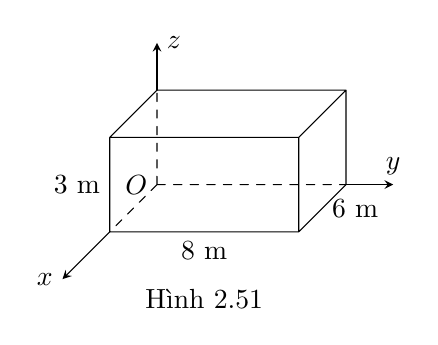
\begin{tikzpicture}[line cap=round,line join=round, >=stealth,scale=0.6]
			\path (0,0)coordinate[label=left:$O$](O) (-1,-1)coordinate(B) (4,0)coordinate(D) (3,-1)coordinate(C) (0,2)coordinate(O') (-1,1)coordinate(B') (3,1)coordinate(C') (4,2)coordinate(D') (0,3)coordinate[label=right:$z$](E) (5,0)coordinate[label=above:$y$](F) (-2,-2)coordinate[label=left:$x$](G) (-1,0)coordinate[label=left:$3$ m](H) (1,-1)coordinate[label=below:$8$ m](I)
			(3.5,-0.5)coordinate[label=right:$6$ m](K) (1,-2)coordinate[label=below:Hình 2.51](M) ;
			\draw (B)--(B')--(C')--(C)--cycle (O')--(B') (O')--(D') (C')--(D') (D')--(D) (D)--(C);
			\draw[dashed] (O)--(B) (O)--(D) (O)--(O');
			\draw[->] (B)--(G);
			\draw[->] (O')--(E);
			\draw[->] (D)--(F);
		\end{tikzpicture}
	}
	\loigiai{
		\immini{Gọi các điểm $B(3;0;0)$, $C(3;6;0)$, $D(0;6;0)$ như hình vẽ.\\
			$N$ là trung điểm $OC$, $N'$ là hình chiếu của $N$ lên mặt phẳng trần nhà.\\
			Suy ra $N'$ là điểm treo đèn.\\
			Ta có $N$ có tọa độ là $\left(\dfrac{0+3}{2};\dfrac{0+6}{2};\dfrac{0+0}{2}\right)$, suy ra $N\left(\dfrac{3}{2};3;0\right)$.\\
			Suy ra $N'\left(\dfrac{3}{2};3;3\right)$.\\
			Vậy tọa độ của điểm treo đèn là $\left(\dfrac{3}{2};3;3\right)$.
		}
		{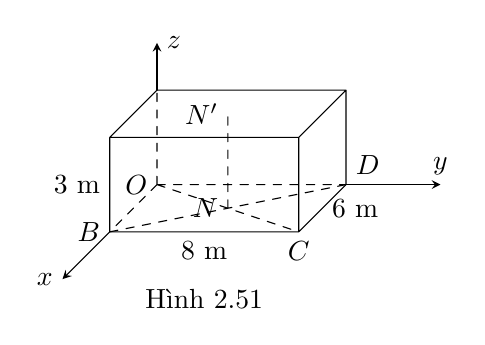
\begin{tikzpicture}[line cap=round,line join=round, >=stealth,scale=0.6]
				\path (0,0)coordinate[label=left:$O$](O) (-1,-1)coordinate[label=left:$B$](B) (4,0)coordinate[label=above right:$D$](D) (3,-1)coordinate[label=below:$C$](C) (0,2)coordinate(O') (-1,1)coordinate(B') (3,1)coordinate(C') (4,2)coordinate(D') (0,3)coordinate[label=right:$z$](E) (6,0)coordinate[label=above:$y$](F) (-2,-2)coordinate[label=left:$x$](G) (-1,0)coordinate[label=left:$3$ m](H) (1,-1)coordinate[label=below:$8$ m](I)
				(3.5,-0.5)coordinate[label=right:$6$ m](K) (1,-2)coordinate[label=below:Hình 2.51](M);
				\coordinate[label=left:$N$] (N) at (intersection cs:first line={(O)--(C)}, second line={(B)--(D)});
				\coordinate[label=left:$N'$] (N') at (intersection cs:first line={(O')--(C')}, second line={(B')--(D')});
				\draw (B)--(B')--(C')--(C)--cycle (O')--(B') (O')--(D') (C')--(D') (D')--(D) (D)--(C);
				\draw[dashed] (O)--(B) (O)--(D) (O)--(O') (O)--(C) (B)--(D) (N)--(N');
				\draw[->] (B)--(G);
				\draw[->] (O')--(E);
				\draw[->] (D)--(F);
		\end{tikzpicture}}
	}
\end{bt}

% #1251 | Archive/2024/0. [LVH] BG - 12 New - 4in1-20240625T224301Z-001/0. [LVH] BG - 12 New - 4in1/data/data_C5/Bai2-Dang1.tex | mã gốc 2H3N3-1
\begin{vd}[CTST, Mức độ 1]%[2H3N3-1]
	Trong không gian $Oxyz$, cho hình chóp $O.ABC$ có $A\left( 2;0;0 \right),B\left( 0;4;0 \right)$ và $C\left( 0;0;7 \right)$.
	\begin{enumerate}
		\item Tìm tọa độ một vectơ chỉ phương của đường thẳng $AB$, $AC$.
		\item Vectơ $\overrightarrow{v}=\left( -1;2;0\right)$ có là vectơ chỉ phương của đường thẳng $AB$ không?
	\end{enumerate}
	\loigiai{
		\immini{\begin{enumerate}
				\item Ta có $\overrightarrow{AB}=\left( -2;4;0 \right)$ là một vectơ chỉ phương của đường thẳng $AB$; $\overrightarrow{AC}=\left( -2;0;7 \right)$ là một vectơ chỉ phương của đường thẳng $AC$.
				\item Vì $\overrightarrow{v}=\left( -1;2;0 \right)=\dfrac{1}{2}\overrightarrow{AB}$ nên $\overrightarrow{v}$ là một vectơ chỉ phương của đường thẳng $AB$.
		\end{enumerate}}{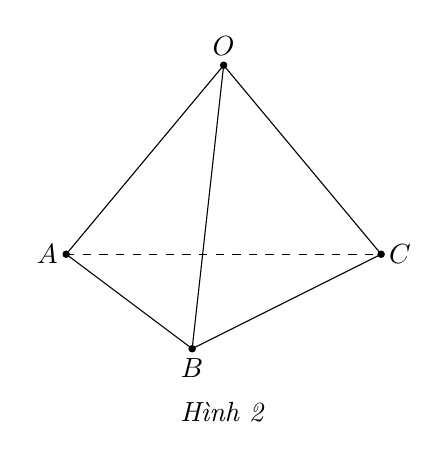
\begin{tikzpicture}[xscale=0.8,yscale=0.8]
				\path
				(0,0) coordinate (A)
				(2,-1.5) coordinate (B)
				(5,0) coordinate (C)
				(2.5,3) coordinate (O)
				;
				\draw[dashed] (A)--(C)
				;
				\draw (A)--(B) (A)--(O) (C)--(B) (B)--(O) (C)--(O)
				;
				\foreach \x/\g in {O/90, A/180, B/-90, C/0} \path (\x) circle (.05) +(\g:.3) node {$\x$}
				;
				\draw (2.5,-2.5) node{\textit{Hình 2}}
				;
				\foreach \x/\g in {O/90, A/90, B/90, C/90} \draw[fill=black] (\x) circle (.05) +(\g:.3) node {}
				;
		\end{tikzpicture}}
	}
\end{vd}

% #1252 | Archive/2024/0. [LVH] BG - 12 New - 4in1-20240625T224301Z-001/0. [LVH] BG - 12 New - 4in1/data/data_C5/Bai2-Dang1.tex | mã gốc 2H3N3-1
\begin{vd}[CTST, Mức độ 1]%[2H3N3-1]
	Trong không gian $Oxyz$, cho hình lăng trụ tam giác $ABC. A^\prime B^\prime  C^\prime $ với $A\left( 1;2;1 \right),B\left( 7;5;3 \right)$, $C\left( 4;2;0 \right), A^\prime \left( 4;9;9 \right)$. Tìm toạ độ một vectơ chỉ phương của mỗi đường thẳng $AB, A^\prime C^\prime $ và $B B^\prime $.
	\loigiai{
		Một vectơ chỉ phương của $AB$ là $\vec{AB}=\left(6;3;2\right)$.\\
		Một vectơ chỉ phương của $A'C'$ là $\vec{A'C'}=\vec{AC}=\left(3;0;-1\right)$.\\
		Một vectơ chỉ phương của $BB'$ là $\vec{BB'}=\vec{AA'}=\left(3;7;8\right)$.\\
	}
\end{vd}

% #1254 | Archive/2024/0. [LVH] BG - 12 New - 4in1-20240625T224301Z-001/0. [LVH] BG - 12 New - 4in1/data/data_C5/Bai2-Dang1.tex | mã gốc 2H3N3-1
\begin{vd}[KNTT, Mức độ 1]%[2H3N3-1]
	\immini{Cho hình hộp $A B C D \cdot A'B'C'D'$. Hãy chỉ ra các vectơ chỉ phương của đường thẳng $B C'$ mà điểm đầu và điểm cuối của vectơ đó đều là các đỉnh của hình hộp $A B C D \cdot A'B'C'D'$.
	}{
		\begin{tikzpicture}[scale=1, font=\footnotesize, line join=round, line cap=round,>=stealth]
			\path (-0.5,3) coordinate (h) (0,0)coordinate (B) (1.5,0) coordinate (C) (3.7,1) coordinate (D) ($(B)+(D)-(C)$) coordinate (A);
			\foreach \p in {A,B,C,D}\path ($(\p)+(h)$) coordinate (\p');
			\path ($(A)!(D')!(D)$) coordinate (H);
			\draw (A')--(B')--(B)--(C)--(D)--(D')--cycle (B')--(C')--(D') (C)--(C');
			\draw[dashed] (C')--(B)--(A)--(D) (A)--(A') (D')--(A);
			\foreach \p/\g in {A/150,B/240,C/-60,D/0,A'/90,B'/180,C'/-30,D'/45} \fill[black] (\p) circle(1pt)+(\g:0.3) node{$\p$};
			\draw ($(B)!0.5!(D)$)++(-90:1) node{Hình $5.24$};
		\end{tikzpicture}
	}
	\loigiai{
		Đường thẳng $BC'$ nhận các vectơ $\overrightarrow{BC'}, \overrightarrow{C'B}, \overrightarrow{AD'}, \overrightarrow{D'A}$ là các vectơ chỉ phương.
	}
\end{vd}

% #1255 | Archive/2024/0. [LVH] BG - 12 New - 4in1-20240625T224301Z-001/0. [LVH] BG - 12 New - 4in1/data/data_C5/Bai2-Dang1.tex | mã gốc 2H3N3-1
\begin{vd}[KNTT, Mức độ 1]%[2H3N3-1]
	\immini{Cho hình lăng trụ $A B C . A'B'C'(H .5 .25)$. Trong các vectơ có điểm đầu và điểm cuối đều là đỉnh của hình lăng trụ, những vectơ nào là vectơ chỉ phương của đường thẳng $AB$?
	}{
		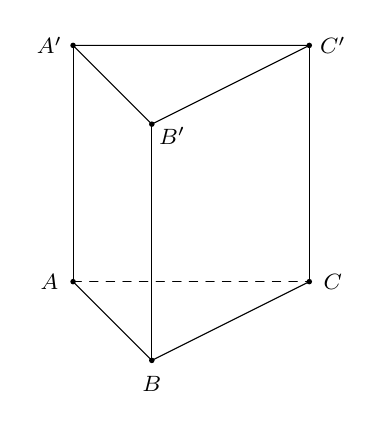
\begin{tikzpicture}[scale=1, font=\footnotesize, line join=round, line cap=round,>=stealth]
			\path (0,0)coordinate (A) (3,0) coordinate (C) (1,-1) coordinate (B) (0,3) coordinate (h);
			\foreach \p in {A,B,C} {\draw (\p)--(\p)--+(h) coordinate (\p');}
			\draw (A')--(B')--(C')--cycle (A)--(B)--(C);
			\draw[dashed] (A)--(C);
			\foreach \p/\g in {A/180,B/-90,C/0,A'/180,B'/-30,C'/0} \fill[black] (\p) circle(1pt)+(\g:0.3) node{$\p$};
		\end{tikzpicture}
	}
	\loigiai{Các véc-tơ chỉ phương của đường thẳng $AB$ là $\overrightarrow{AB}$, $\overrightarrow{A'B'}$.}
\end{vd}

% #1256 | Archive/2024/0. [LVH] BG - 12 New - 4in1-20240625T224301Z-001/0. [LVH] BG - 12 New - 4in1/data/data_C5/Bai2-Dang1.tex | mã gốc 2H3N3-1
\begin{bt}%[2H3N3-1][Mức độ 1]
	Trong không gian $Oxyz$, cho ba điểm $A(1;0;6)$, $B(0;2;-1)$, $C(2;4;3)$. Tìm một véc-tơ chỉ phương của đường thẳng chứa trung tuyến $AM$ của tam giác $ABC$.
	\loigiai{
		Gọi $M$ là trung điểm của $BC \Rightarrow M(1;3;1)$.\\
		Ta có $\overrightarrow{AM}=(0;3;-5)=-\overrightarrow{u}_2$, với $\overrightarrow{u}_2=(0;-3;5)$.
	}
\end{bt}

% #1258 | Archive/2024/0. [LVH] BG - 12 New - 4in1-20240625T224301Z-001/0. [LVH] BG - 12 New - 4in1/data/data_C5/Bai2-Dang1.tex | mã gốc 2H3H3-1
\begin{bt}%[2H3H3-1][Mức độ 2]
	Trong không gian $Oxyz$, cho ba điểm $A(-3;2;2), B(0;-1;2), C(3;1;-3)$. Gọi $\Delta$ là đường thẳng đi qua $C$ và song song với đường thẳng $AB$. Tìm một véc-tơ chỉ phương của $\Delta$.
	\loigiai{
		Ta có $\overrightarrow{AB}=(3;-3;0)$.\\
		Vì $\Delta$ song song với đường thẳng $AB$ nên $\overrightarrow{AB}$ là một véc-tơ chỉ phương của $\Delta$.\\
		Ta chọn $\overrightarrow{u}=-\dfrac{1}{3}\overrightarrow{AB}=\left(-1;1;0\right)$ là vec-tơ chỉ phương của $\Delta$.
	}
\end{bt}

% #1328 | Archive/2024/0. [LVH] BG - 12 New - 4in1-20240625T224301Z-001/0. [LVH] BG - 12 New - 4in1/data/data_C5/Bai1-Dang4-Vi-tri-tuong-doi-cua-hai-MP.tex | mã gốc 2H3B2-7
\begin{bt}%[12 bài giảng 4 trong 1, Hiếu Mai]%[2H3B2-7]
	Xét vị trí tương đối của hai mặt phẳng sau
	\begin{listEX}
		\item $ (\alpha_{1})\colon x+2y-3z+2=0 $ và $ (\alpha_{2})\colon -2x-4y+6x-5=0 $;
		\item  $ (\beta_{1})\colon x+2z-5=0 $ và $ (\beta_2) \colon 4x-3y-2z+1=0$;
		\item $ (\gamma_1)\colon x-2y+z+3=0 $ và $ (\gamma_2)\colon 2x-4y+3z+2=0 $
	\end{listEX}
	\loigiai{
		\begin{listEX}
			\item Ta có $ \dfrac{1}{-2}=\dfrac{2}{-4}=\dfrac{-3}{6}\ne \dfrac{2}{-5} $ nên $ (\alpha_1) \parallel (\alpha_2)$;
			\item Véc-tơ pháp tuyến của $ (\beta_1) $ là $ \overrightarrow{n}_1=(1;0;2) $, véc-tơ pháp tuyến của $ (\beta_2) $ là $ \overrightarrow{n}_2=(4;-3;-2) $.\\
			Ta có $ \overrightarrow{n}_1\cdot\overrightarrow{n}_2=4\cdot1+0\cdot(-3)+2\cdot(-2) =0$ nên $ (\beta_1)\perp (\beta_2) $;
			\item Ta có $ \dfrac{1}{2}\ne \dfrac{1}{3} $ nên $ (\gamma_1) $ cắt $ (\gamma_2) $.\\
			Véc-tơ pháp tuyến của $ (\gamma_1) $ là $ \overrightarrow{n}_1=(1;-2;1) $, véc-tơ pháp tuyến của $ (\gamma_2) $ là $ \overrightarrow{n}_2=(2;-4;3) $.\\
			Ta có $ \overrightarrow{n}_1\cdot\overrightarrow{n}_2=1\cdot2+(-2)\cdot(-4)+1\cdot3 =13\ne 0$ nên $ (\gamma_1)$ không vuông góc $ (\gamma_2) $.
		\end{listEX}
	}	
\end{bt}

% #1340 | Archive/2024/0. [LVH] BG - 12 New - 4in1-20240625T224301Z-001/0. [LVH] BG - 12 New - 4in1/data/data_C5/Bai1-Dang1-Tich-co-huong.tex | mã gốc 2H2H2-5
\begin{vd}[Mức độ 2]%[2H2H2-5]%[Phạm Hoàng Điệp]
	Tính thể tích tứ diện $ ABCD $ với $ A(2;1;0) ,B(0; 3;0), C(0;-2;1), D(2;1;1)$ (làm tròn kết quả đến hàng phần trăm).
\SA{$1{,} 67$}
	\loigiai{
		Ta có: $ \heva{& \vv{AB}=(-2;2;0) \\ & \vv{AC}=(-2;-3;1)} \Rightarrow \left [\vv{AB},\vv{AC}\right ]=(2;2;10)$ và $\vv{AD}=(0;0;1) $.\\
		$ \Rightarrow \left [\vv{AB},\vv{AC}\right ]\cdot \vv{AD}=2\cdot 0+2 \cdot 0 + 10 \cdot 1 =10 $\\
		$ \Rightarrow $ \fbox{$ V_{ABCD}=\dfrac{1}{6} \left | \left [\vv{AB},\vv{AC}\right ] \cdot \vv{AD}\right |$}\,$  =\dfrac{1}{6} \cdot |10|=\dfrac{5}{3} \approx 1{,} 67$.
	}
\end{vd}

% #1341 | Archive/2024/0. [LVH] BG - 12 New - 4in1-20240625T224301Z-001/0. [LVH] BG - 12 New - 4in1/data/data_C5/Bai1-Dang1-Tich-co-huong.tex | mã gốc 2H2V2-5
\begin{bt}[Mức độ 3]%[2H2V2-5]%[Phạm Hoàng Điệp]
	Trong không gian $Oxyz$, cho bốn điểm $A\left(1;0;0\right)$,  $B\left(0;1;0\right)$,  $C\left(0;0;1\right)$,  $D\left(- 2;1; -1\right)$.
	\begin{enumerate}
		\item Chứng minh $A$, $B$, $C$, $D$  là bốn đỉnh của tứ diện. Tính thể tích của tứ diện này
		\dapso{ $V = \dfrac{1}{2}$}.
		\item  Tính diện tích tam giác $BCD$. Từ đó suy ra độ dài đường cao của tứ diện vẽ từ $A$
		\dapso{$S_{\triangle BCD} = \sqrt{5}$; $h = \dfrac{3\sqrt{5}}{10}$}.
	\end{enumerate}
	\loigiai{
		\begin{enumerate}
			\item  Ta có $\overrightarrow{AB} = \left(-1; 1; 0\right)$, $\overrightarrow{AC} = \left(-1; 0; 1\right)$ và $\overrightarrow{AD} = \left(-3; 1; -1\right)$.\\
			Khi đó $\left[\overrightarrow{AB}, \overrightarrow{AC}\right] = \left(1; 1; 1\right)$ nên $\left[\overrightarrow{AB}, \overrightarrow{AC}\right]\cdot \overrightarrow{AD} = 1\cdot \left(- 3\right) + 1\cdot 1 + 1\cdot \left(- 1\right) = -3\neq 0$.\\
			Do đó $A$, $B$, $C$, $D$  là bốn đỉnh của tứ diện.\\
			Gọi $V$ là thể tích của tứ diện ta có $V = \dfrac{1}{6}\left\vert\left[\overrightarrow{AB}, \overrightarrow{AC}\right]\cdot \overrightarrow{AD}\right\vert = \dfrac{1}{6}\left\vert - 3\right\vert = \dfrac{1}{2}$.\\
			Vậy thể tích của tứ diện là $\dfrac{1}{2}$.
			\item Ta có $S_{\triangle BCD} =  \dfrac{1}{2}\left\vert\left[\overrightarrow{BC}, \overrightarrow{BD}\right]\right\vert$ mà $ \left[\overrightarrow{BC}, \overrightarrow{BD}\right] = \left(- 1; -2; -2 \right)$.\\
			Do đó $S_{\triangle BCD} = \dfrac{1}{2}\sqrt{(-1)^2 + (-2)^2 + (-2)^2} = \dfrac{3}{2}$.\\
			Gọi $h$ là độ dài đường cao của tứ diện vẽ từ $A$.\\
			Ta có $V = \dfrac{1}{3}\cdot h\cdot S_{\triangle BCD}\Leftrightarrow \dfrac{1}{2} = \dfrac{1}{3}\cdot h\cdot \dfrac{3}{2}\Leftrightarrow h = 1$.
				\end{enumerate}
}
\end{bt}

% #1342 | Archive/2024/0. [LVH] BG - 12 New - 4in1-20240625T224301Z-001/0. [LVH] BG - 12 New - 4in1/data/data_C5/Bai1-Dang1-Tich-co-huong.tex | mã gốc 2H2H2-5
\begin{bt}[Mức độ 2]%[2H2H2-5]%[Phạm Hoàng Điệp]
	Cho $ A(1 ; 2 ;-1), B(0 ;-2 ; 3) $. Tính độ dài đường cao $ AH $ hạ từ đỉnh $ A $ của tam giác $ OAB $.
	\loigiai{
		\immini
		{
			$S_{\triangle ABC}=\dfrac{1}{2}\cdot \left | \left [\vv{OA},\vv{OB}\right ] \right | =\dfrac{AH \cdot BO}{2} \Rightarrow AH=\dfrac{\left | \left [\vv{OA},\vv{OB}\right ] \right |}{OB}$\\
			Có $ \heva{& \vv{OA}=(1;2;-1) \\ & \vv{OB}=(0;-2;3)} \Rightarrow \left [\vv{OA},\vv{OB}\right ]=(4;-3;-2)$.	\\
			Suy ra $ \left | \left [\vv{OA},\vv{OB}\right ] \right |=\sqrt{29} $  và $ OB=\sqrt{13} $.\\
			Dó đó $ AH=\dfrac{\left | \left [\vv{OA},\vv{OB}\right ] \right |}{OB}=\dfrac{\sqrt{29}}{\sqrt{13}}=\dfrac{\sqrt{377}}{13} $.
		}
		{
			\begin{tikzpicture}[scale=1, font=\footnotesize, line join=round, line cap=round, >=stealth]
				\path
				(1,2.5) coordinate (A) node[above]{$ A(1;2;-1)$}
				(0,0) coordinate (O)node[below]{$ O(0;0;0) $}
				(4,0) coordinate (B) node[below]{$ B(0;-2;3) $}
				($(O)!(A)!(B)$) coordinate (H) node[below]{$ H $}
				;
				
				\draw (A)--(O)--(B)--cycle
				pic [draw=red,fill=yellow!30,angle radius=4mm] {right angle = A--H--B};;
				\draw[red,line width=1pt] (A)--(H);
				
				\foreach \p/\r in {A,O,B,H}
				\draw[fill=white] (\p) circle (1.5pt) ;
			\end{tikzpicture}
		}
		
	}
\end{bt}

% #1343 | Archive/2024/0. [LVH] BG - 12 New - 4in1-20240625T224301Z-001/0. [LVH] BG - 12 New - 4in1/data/data_C5/Bai1-Dang1-Tich-co-huong.tex | mã gốc 2H2H2-5
\begin{bt}[Mức độ 2]%[2H2H2-5]%[Phạm Hoàng Điệp]
	Cho hình hộp $ABCD.A'B'C'D'$, có toạ độ các đỉnh $A\left(0;0;1\right),B\left(0;2;1\right),D\left(3;0;1\right),A'\left(0;0;0\right)$. Tính thể tích của khối hộp đã cho.\\
		\dapso{$C\left(3;2;1\right),B'\left(0;2;0\right),C'\left(3;2;0\right),D'\left(3;0;0\right),V_{ABCD..A'B"C"D"}=6$}
	\loigiai{
			Ta có $\overrightarrow{AA'}\left(0;0;-1\right)$,  $\overrightarrow{AB}\left(0;2;0\right),\overrightarrow{AD}\left(3;0;0\right)\Rightarrow \left[\overrightarrow{AB};\overrightarrow{AD}\right]=\left(0;0;-6\right)$.\\
			Thể tích của khối hộp $ABCD.A'B'C'D'$ là $$V_{ABCD.A'B'C'D'}=\left| \left[\overrightarrow{AB};\overrightarrow{AD}\right]\cdot  \overrightarrow{AA'}\right|=\left|0+0+(-6)\cdot (-1)\right|=6.$$
	}
\end{bt}

% #1344 | Archive/2024/0. [LVH] BG - 12 New - 4in1-20240625T224301Z-001/0. [LVH] BG - 12 New - 4in1/data/data_C5/Bai1-Dang1-Tich-co-huong.tex | mã gốc 2H2V2-5
\begin{bt}[Mức độ 3]%[2H2V2-5]%[Phạm Hoàng Điệp]
	Cho tứ diện $ABCD$ với $A(2;1;-1), B(3;0;1), C(2;-1;3)$ và $D\in Oy$. Biết thể tích của tứ diện $ABCD$ bằng $5$ (đvtt). Tìm tọa độ đỉnh $D$.
	\dapso{$D(0;-7;0)$ hoặc $D(0;8;0)$}
	\loigiai{Gọi $D(0,b,0)\in Oy$.
		Ta có $V_{ABCD}=\dfrac{1}{6}\left|\left[\overrightarrow{AB};\overrightarrow{AC}\right]\cdot \overrightarrow{AD}\right|$. \\  Mà $\overrightarrow{AB}=(1;-1;2)$, $\overrightarrow{AC}=(0;-2;4)$ $\overrightarrow{AD}=(-2;b-1;1)$.\\
		 Khi đó $\left[\overrightarrow{AB};\overrightarrow{AC}\right]=(0;-4;-2)$ và $\left[\overrightarrow{AB};\overrightarrow{AC}\right]\cdot \overrightarrow{AD}=-4(b-1)-2=-4b+2$. \\
		Theo bài ra $$V_{ABCD} = 5 \Leftrightarrow \dfrac{1}{6}|-4b+2|=5\Leftrightarrow \hoac{& -4b+2=30 \\ & -4b+2=-30}\Leftrightarrow\hoac{&  b=-7 \\ & b=8.}$$
		Suy ra $D(0;-7;0)$ hoặc $D(0;8;0)$.
	}
\end{bt}

% #1345 | Archive/2024/0. [LVH] BG - 12 New - 4in1-20240625T224301Z-001/0. [LVH] BG - 12 New - 4in1/data/data_C5/Bai1-Dang1-Tich-co-huong.tex | mã gốc 2H2V2-5
\begin{bt}[Mức độ 3]%[2H2V2-5]%[Phạm Hoàng Điệp]
	Cho $ A(a;-1;6), B(-3 ;-1 ;-4),  C(5 ;-1 ; 0) $ và $ D(1;2;1) $. Tìm toạ độ điểm $A$ để thể tích của tứ diện  $ ABCD $ bằng $ 30 $.
	\loigiai{
		Ta có $ \heva{& \vv{DB}=(-4;-3;-5) \\ & \vv{DC}=(4;-3;-1)} \Rightarrow \left [\vv{DB},\vv{DC}\right ]=(-12;-24;24)$	\\
		Lại có $ \vv{DA}=(a-1;-3;5) $.\\ Để $ V_{ABCD}=30 \Leftrightarrow \dfrac{1}{6} \cdot \left | \left [\vv{DB},\vv{DC}\right ] \cdot \vv{DA}\right |=30 \Leftrightarrow   \left| -12a+204\right|=180 \Leftrightarrow \hoac{& a=32 \\ & a=2.}$\\
		Vậy $A(32;-1;6)$ hoặc $A(2;-1;6)$.
		
	}
\end{bt}

% #1351 | Archive/2024/0. [LVH] BG - 12 New - 4in1-20240625T224301Z-001/0. [LVH] BG - 12 New - 4in1/data/data_C5/Bai1-Dang1-Tich-co-huong.tex | mã gốc 2H2V2-5
\begin{ex}[Mức độ 3]%[2H2V2-5]%[Phạm Hoàng Điệp]
	Trong không gian $Oxyz$, cho tứ diện $ABCD$ với $A(-1; -2; 4)$, $B(-4; -2; 0)$, $C(3; -2; 1)$ và $D(1; 1; 1)$. Tính độ dài đường cao của tứ diện $ABCD$ kẻ từ đỉnh $D$.
\SA{2}
	\loigiai
	{ Ta có $\heva{&\vv{AB}=(-3;0;-4)\\&\vv{AC}=(4;0;-3)}\Rightarrow \left[\vv{AB},\vv{AC}\right]=(0;-25;0)$ và $\vv{AD} = (2;3;-3)$.\\
		Diện tích tam giác $ABC$ là $S_{\triangle ABC}=\dfrac{1}{2}\cdot\left|\left[\overrightarrow{AB},\overrightarrow{AC}\right]\right|=\dfrac{25}{2}$.\\
		Thể tích tứ diện $V_{ABCD}=\dfrac{1}{6}\left|\left[\overrightarrow{AB},\overrightarrow{AC}\right]\cdot \overrightarrow{AD}\right|=\dfrac{25}{2}.$\\
		Vậy độ dài đường cao $h=d\left(D,\left(ABC\right)\right)=\dfrac{3V_{ABCD}}{S_{\Delta ABC}}=3.$	
	}
\end{ex}

% #1352 | Archive/2024/0. [LVH] BG - 12 New - 4in1-20240625T224301Z-001/0. [LVH] BG - 12 New - 4in1/data/data_C5/Bai1-Dang1-Tich-co-huong.tex | mã gốc 2H2H2-5
\begin{ex}[Mức độ 2]%[2H2H2-5]%[Phạm Hoàng Điệp]
	Tính diện tích tam giác $ ABC $ với $ A(1;0;0),B(0;0;1), $ và $ C(2;1;1) $ (làm tròn kết quả đến hàng phần chục).
	\SA{$1{,}2$}
	\loigiai{
		Có $ \heva{& \vv{AB}=(-1;0;1) \\ & \vv{AC}=(1;1;1)} \Rightarrow \left [\vv{AB},\vv{AC}\right ]=(-1;2;-1)$	\\
		$ \Rightarrow$ $ S_{\triangle ABC}=\dfrac{1}{2}\cdot \left | \left [\vv{AB},\vv{AC}\right ] \right | = \dfrac{1}{2} \sqrt{(-1)^2+2^2+(-1)^2} =\dfrac{\sqrt{6}}{2} \approx 1{,}2 $.
	}
\end{ex}

% #1353 | Archive/2024/0. [LVH] BG - 12 New - 4in1-20240625T224301Z-001/0. [LVH] BG - 12 New - 4in1/data/data_C5/Bai1-Dang1-Tich-co-huong.tex | mã gốc 2H2H2-5
\begin{ex}[Mức độ 2]%[2H2H2-5]%[Phạm Hoàng Điệp]
	Trong không gian $Oxyz$, cho tứ diện $ABCD$ với $A(2;0 ; 0)$, $B(0; 2; 0)$, $C(0; 0; 2)$ và $D(-2; 1; -1)$. Thể tích của tứ diện $ABCD$ bằng bao nhiêu? (kết quả làm tròn đến hàng phần trăm).
	\SA{ $2{,}67$}
	\loigiai
	{
		Ta có $ \heva{& \vv{AB}=(-2;2;0) \\ & \vv{AC}=(-2;0;2)} \Rightarrow \left [\vv{AB},\vv{AC}\right ]=(4;4;4)$ và $\vv{AD}=(-4;1;-1) $.\\
	$ \Rightarrow \left [\vv{AB},\vv{AC}\right ]\cdot \vv{AD}=4\cdot (-4)+4 \cdot 1 + 4 \cdot (-1) = -16 $\\
	$ \Rightarrow  V_{ABCD}=\dfrac{1}{6} \left | \left [\vv{AB},\vv{AC}\right ] \cdot \vv{AD}\right | =\dfrac{1}{6} \cdot |-16|=\dfrac{8}{3}\approx 2{,}67 $.
	}
\end{ex}

% #1354 | Archive/2024/0. [LVH] BG - 12 New - 4in1-20240625T224301Z-001/0. [LVH] BG - 12 New - 4in1/data/data_C5/Bai1-Dang1-Tich-co-huong.tex | mã gốc 2H2H2-5
\begin{ex}[Mức độ 2]%[2H2H2-5]%[Phạm Hoàng Điệp]
	Tính diện tích hình bình hành $ ABCD $ với $ A(1;1;1), B(2;3;4), C(6;5;2) $ (làm tròn kết quả đến hàng phần mười).
	\SA{$18{,}2$}
	\loigiai{
		Ta có $  \heva{& \vv{AB}=(1;2;3) \\ & \vv{AC}=(5;4;1).} $\\
		Suy ra $ \left [\vv{AB},\vv{AC}\right ]=(-10;14;-6) $.\\
		Diện tích hình bình hành $ S_{ABCD}=\left | \left [\vv{AB},\vv{AC}\right ] \right | =\sqrt{(-10)^{2}+14^{2}+(-6)^{2}}=2\sqrt{83}\approx 18{,}2 $.
	}
\end{ex}

% #1355 | Archive/2024/0. [LVH] BG - 12 New - 4in1-20240625T224301Z-001/0. [LVH] BG - 12 New - 4in1/data/data_C5/Bai1-Dang1-Tich-co-huong.tex | mã gốc 2H2V2-5
\begin{ex}[Mức độ 3]%[2H2V2-5]%[Phạm Hoàng Điệp]
	Cho tam giác $ ABC $ có $ A(1;0;1) , B(0;2;3)$ và $ C(2;1;0) $. Tính chiều cao $ CH $ (làm tròn kết quả đến hàng phần chục).
	\SA{$1{,}7$}
	\loigiai{
		\immini
		{
			$S_{\triangle ABC}=\dfrac{1}{2}\cdot \left | \left [\vv{AC},\vv{AB}\right ] \right | =\dfrac{AB \cdot CH}{2} \Rightarrow CH=\dfrac{\left | \left [\vv{AC},\vv{AB}\right ] \right |}{AB}$\\
			Có $ \heva{& \vv{AC}=(1;1;-1) \\ & \vv{AB}=(-1;2;2)} \Rightarrow \left [\vv{AC},\vv{AB}\right ]=(4;-1;3)$.	\\
			Suy ra $ \left | \left [\vv{AC},\vv{AB}\right ] \right |=\sqrt{26} $  và $ AB=3 $.\\
			Dó đó $ CH=\dfrac{\left | \left [\vv{AC},\vv{AB}\right ] \right |}{AB}=\dfrac{\sqrt{26}}{3}=\dfrac{\sqrt{26}}{3}\approx 1{,}7 $.
		}
		{
			\begin{tikzpicture}[scale=1, font=\footnotesize, line join=round, line cap=round, >=stealth]
				\path
				(1,3) coordinate (A) node[shift={(90:3mm)}]{$A(1;0;1)$}
				(0,0) coordinate (B)node[shift={(270:3mm)}]{$B(0;2;3)$}
				(4,0) coordinate (C)node[shift={(-90:3mm)}]{$C(2;1;0)$}
				($(A)!(C)!(B)$) coordinate (H)node[shift={(180:3mm)}]{$H$}
				;
				
				\draw (A)--(B)--(C)--cycle
				pic [draw=red,fill=yellow!30,angle radius=4mm] {right angle = C--H--A};
				\draw[red,line width=1pt] (C)--(H);
				\foreach \p/\r in {A,B,C,H}
				\draw[fill=white] (\p) circle (1.5pt) ;
			\end{tikzpicture}
		}
		
	}
\end{ex}

% #1509 | Archive/2024/0. [LVH] BG - 12 New - 4in1-20240625T224301Z-001/0. [LVH] BG - 12 New - 4in1/data/data_C2/Bai-2-Dang3-ToaDoDiemDB.tex | mã gốc 2H2N2-2
\begin{vd}[KNTT, Mức độ 1]%[BG -12 New -4in1, Hector Tran]%[2H2N2-2]
	\immini{Hình 1 minh hoạ một hệ toạ độ $Oxyz$ trong không gian cùng với các hình vuông có cạnh bằng $1$ đơn vị. Tìm toạ độ của điểm $M$.	
	}{
		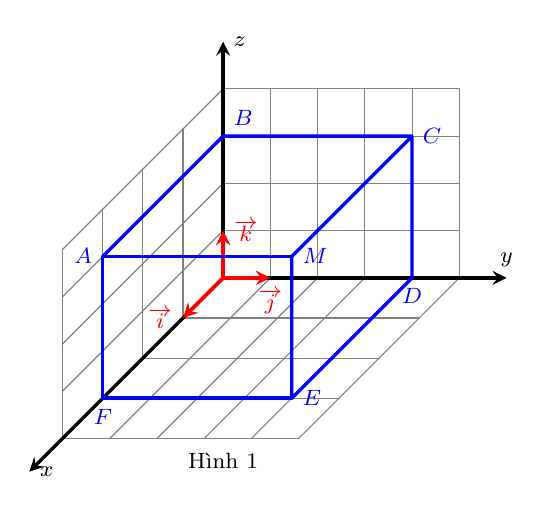
\begin{tikzpicture}[scale=0.6, font=\footnotesize, line join=round, line cap=round, >=stealth]
			%Giới hạn các trục tọa độ
			\def\tl{1.2} %tỉ lệ của trục tung
			\def\hoanh{5} \def\cao{4} \def\tung{4}
			\def\goc{-135}
			%\pgfmathsetmacro\tung{4*\tl}
			%Vẽ lưới các mặt phẳng tọa độ
			\foreach \x in {1,2,...,5}
			{
				\draw[thin,gray] (0:\x)--++(90:\cao);
				\draw[thin,,gray] (0:\x)--++(\goc:\tung*\tl);
			}
			\foreach \y in {1,2,3,4}
			{
				\draw[thin,gray] (\goc:\y*\tl)--++(0:\hoanh);
				\draw[thin,gray]	(\goc:\y*\tl)--++(90:\cao);
			}
			\foreach \z in {1,2,3,4}
			{
				\draw[thin,gray] (90:\z)--++(0:\hoanh);
				\draw[thin,gray]	(90:\z)--++(\goc:\tung*\tl);
			}
			%Vẽ các trục tọa độ
			\draw[line width=1.2,->,black] (0:0)--++(0:\hoanh+1) node[above]{$y$};
			\draw[line width=1.2,->,black] (0:0)--++(
			\goc:\tung*\tl+1) node[right]{$x$};
			\draw[line width=1.2,->,black] (0:0)--++(90:\cao+1) node[right]{$z$};
			%Vẽ các vectơ đơn vị
			\draw[line width=1.3,->,red] (0:0)--++(0:1) node[below]{$\overrightarrow{j}$};
			\draw[line width=1.3,->,red] (0:0)--++(\goc:\tl) node[left]{$\overrightarrow{i}$};
			\draw[line width=1.3,->,red] (0:0)--++(90:1) node[right]{$\overrightarrow{k}$};
			%Điểm và các hình chiếu lên mặt phẳng tọa độ
			\draw[line width=1.2,blue] (4,3)node[right]{$C$}--++(\goc:3*\tl) coordinate (N)node[right]{$M$}--++(-90:3)node[right]{$E$}--++(45:3*\tl)node[below]{$D$}--(4,3)--(0,3)node[above right]{$B$}--++(-135:3*\tl);
			\draw[line width=1.2,blue] (N)--++(180:4)node[left]{$A$}--++(-90:3)node[below]{$F$}--++(0:4);
			\path (0,-3.5) node[below]{Hình 1};
	\end{tikzpicture}}
	\loigiai{
		Trong Hình $1$, $ABCM.FODE$ là hình hộp chữ nhật.
		Áp dụng quy tắc hình hộp suy ra
		$$
		\overrightarrow{O M}=\overrightarrow{O F}+\overrightarrow{O D}+\overrightarrow{O B}=3 \vec{i}+4 \vec{j}+3 \vec{k} .
		$$
		Vì vậy, toạ độ của điểm $M$ là $(3 ; 4 ; 3)$.
	}	
\end{vd}

% #1510 | Archive/2024/0. [LVH] BG - 12 New - 4in1-20240625T224301Z-001/0. [LVH] BG - 12 New - 4in1/data/data_C2/Bai-2-Dang3-ToaDoDiemDB.tex | mã gốc 2H2N2-2
\begin{vd}[KNTT, Mức độ 1]%[BG -12 New -4in1, Hector Tran]%[2H2N2-2]
	\immini{		
		Tìm toạ độ của điểm $N$ trong Hình $2$.
	}{	
		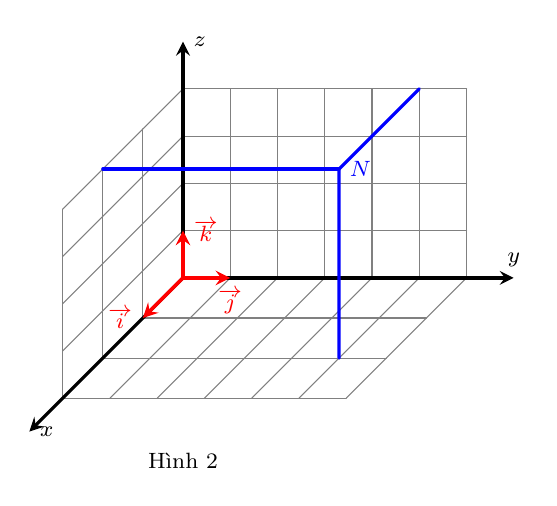
\begin{tikzpicture}[scale=0.6, font=\footnotesize, line join=round, line cap=round, >=stealth]
			%Giới hạn các trục tọa độ
			\def\tl{1.2} %tỉ lệ của trục tung
			\def\hoanh{6} \def\cao{4} \def\tung{3}
			\def\goc{-135}
			%\pgfmathsetmacro\tung{4*\tl}
			%Vẽ lưới các mặt phẳng tọa độ
			\foreach \x in {1,2,...,6}
			{
				\draw[thin,gray] (0:\x)--++(90:\cao);
				\draw[thin,gray] (0:\x)--++(\goc:\tung*\tl);
			}
			\foreach \y in {1,2,3}
			{
				\draw[thin,gray] (\goc:\y*\tl)--++(0:\hoanh);
				\draw[thin,gray]	(\goc:\y*\tl)--++(90:\cao);
			}
			\foreach \z in {1,2,3,4}
			{
				\draw[thin,gray] (90:\z)--++(0:\hoanh);
				\draw[thin,gray] (90:\z)--++(\goc:\tung*\tl);
			}
			%Vẽ các trục tọa độ
			\draw[line width=1.2,->,black] (0:0)--++(0:\hoanh+1) node[above]{$y$};
			\draw[line width=1.2,->,black] (0:0)--++(
			\goc:\tung*\tl+1) node[right]{$x$};
			\draw[line width=1.2,->,black] (0:0)--++(90:\cao+1) node[right]{$z$};
			%Vẽ các vectơ đơn vị
			\draw[line width=1.3,->,red] (0:0)--++(0:1) node[below]{$\overrightarrow{j}$};
			\draw[line width=1.3,->,red] (0:0)--++(\goc:\tl) node[left]{$\overrightarrow{i}$};
			\draw[line width=1.3,->,red] (0:0)--++(90:1) node[right]{$\overrightarrow{k}$};
			%Điểm và các hình chiếu lên mặt phẳng tọa độ
			\draw[line width=1.2,blue] (5,4)--++(\goc:2*\tl) coordinate (N)node[right]{$N$}--++(-90:4);
			\draw[line width=1.2,blue] (N)--++(180:5);
			\path (0,-3.5) node[below]{Hình 2};
		\end{tikzpicture}
	}
	\loigiai{
		Áp dụng quy tắc hình hộp, ta có
		$$
		\overrightarrow{ON}=2 \vec{i}+5 \vec{j}+4 \vec{k} .
		$$
		Vì vậy, toạ độ của điểm $N$ là $(2 ; 5 ; 4)$.
	}	
\end{vd}

% #1511 | Archive/2024/0. [LVH] BG - 12 New - 4in1-20240625T224301Z-001/0. [LVH] BG - 12 New - 4in1/data/data_C2/Bai-2-Dang3-ToaDoDiemDB.tex | mã gốc 2H2N2-2
\begin{vd}[CTST, Mức độ 1]%[BG -12 New -4in1, Hector Tran]%[2H2N2-2]
	\immini{
		Cho hình hộp chữ nhật $OABC.O'B'C'$ có cạnh $OA=4$, $OC=6$, $OO'=3$. Chọn hệ trục toạ độ $Oxyz$ có gốc toạ độ $O$; các điểm $A, C, O'$ lần lượt nằm trên các tia $Ox$, $Oy$, $Oz$. Xác định toạ độ các điểm $A, B, B'$.
	}{
		\begin{tikzpicture}[scale=.7, font=\footnotesize, line join=round, line cap=round, >=Stealth]
			\path 
			(0:0) coordinate (A)
			($(A)+(-135:1)$) coordinate (x)
			(0:4.5) coordinate (B)
			($(A)+(45:2)$) coordinate (O)
			($(O)+(B)-(A)$) coordinate (C)
			($(C)+(0:1)$) coordinate (y)
			($(O)+(90:3)$) coordinate (O')
			($(O')+(90:1)$) coordinate (z)
			($(A)+(90:3)$) coordinate (A')
			($(B)+(90:3)$) coordinate (B')
			($(C)+(90:3)$) coordinate (C')
			($(O)!1/3!(A)$) coordinate (a)
			($(O)!1/3!(O')$) coordinate (o')
			($(O)!1/5!(C)$) coordinate (c)
			;
			\draw[dashed] (A)--(a) (c)--(C) (o')--(O');
			\draw[->,dashed] (O)--(B');
			\draw[->,red,dashed] (O)--(a) node[right]{$\overrightarrow{i}$};
			\draw[->,red,dashed] (O)--(o') node[left=.1]{$\overrightarrow{k}$};
			\draw[->,red,dashed] (O)--(c) node[below]{$\overrightarrow{j}$};
			\draw[->] (O')--(z) node[left]{$z$};
			\draw[->] (C)--(y) node[below]{$y$};
			\draw[->] (A)--(x) node[right]{$x$};
			\draw 	(O')--(A')--(B')--(C')--cycle
			(A')--(A)--(B)--(C) (B')--(B) (C')--(C)
			pic[draw,angle radius=2mm]{right angle=C--O--O'}
			pic[draw,angle radius=2mm]{right angle=A--O--C}
			pic[draw,angle radius=2mm]{right angle=O'--O--A}
			;
			\foreach \x/\g in {A/170,B/-15,C/-30,O/180,A'/170,B'/-15,C'/0,O'/180}
			\draw[fill=black] 	(\x) circle (.5pt)
			($(\g:.5)+(\x)$) node {$\x$};	
		\end{tikzpicture}
	}
	\loigiai{		
		Ta có $\overrightarrow{OA}=4\overrightarrow{i}+0\overrightarrow{j}+0\overrightarrow{k}$, suy ra $A(4; 0; 0)$; \\
		$\overrightarrow{OB}=\overrightarrow{OA}+\overrightarrow{OC}=4\overrightarrow{i}+6\overrightarrow{j}+0\overrightarrow{k}$, suy ra $B(4; 6; 0)$.\\
		$\overrightarrow{OB'}=\overrightarrow{OA}+\overrightarrow{OC}+\overrightarrow{OO'}=4\overrightarrow{i}+6\overrightarrow{j}+3\overrightarrow{k}$, suy ra $B'(4; 6; 3)$.			
	}	
\end{vd}

% #1512 | Archive/2024/0. [LVH] BG - 12 New - 4in1-20240625T224301Z-001/0. [LVH] BG - 12 New - 4in1/data/data_C2/Bai-2-Dang3-ToaDoDiemDB.tex | mã gốc 2H2N2-2
\begin{vd}[KNTT, Mức độ 1]%[BG -12 New -4in1, Hector Tran]%[2H2N2-2]
	\immini{
		Trong không gian $O x y z$, cho hình hộp chữ nhật $A B C D .A' B' C' D'$ có đỉnh $A'$ trùng với gốc $O$ và các đỉnh $D', B', A$ lần lượt thuộc các tia $Ox$, $Oy$, $Oz$ (Hình vẽ). Giả sử đỉnh $C$ có toạ độ là $(2 ; 3 ; 5)$ đối với hệ toạ độ $Oxyz$, hãy tìm toạ độ của các đỉnh $D'$, $B'$, $A$ đối với hệ toạ độ đó.
	}{
		\begin{tikzpicture}[scale=0.6, font=\footnotesize, line join=round, line cap=round, >=stealth]
			\def\bc{4} % cạnh BC
			\def\ba{2} % cạnh BA
			\def\gocB{35} % góc B của đáy
			\coordinate[label=below right:$D'$] (B) at (0,0);
			\coordinate (C) at (\gocB:\ba);
			\coordinate[label=below:$C'$] (A) at (\bc,0);
			\coordinate[label=below right:$B'$] (D) at ($(C)-(B)+(A)$);
			\coordinate[label=above left:$C$] (A') at ($(A)+(90:\bc)$);
			\coordinate[label=left:$D$] (B') at ($(B)-(A)+(A')$);
			\coordinate[label=below right:$A$] (C') at ($(C)-(A)+(A')$);
			\coordinate[label=right:$B$] (D') at ($(D)-(A)+(A')$);
			\draw (B')--(B)(D)--(D')--(A')--(B')--(C')--(D') (B)--(A)--(D) (A)--(A');
			\draw[dashed] (C)--(B)(C)--(D) (C)--(C');
			\foreach \diem in {A,B,C,D,A',B',C',D'}	\fill (\diem)circle(1.0pt);
			\draw[-stealth] (D)--+(0:1)node[right]{$y$};
			\draw[-stealth] (C')--+(90:1)node[above]{$z$};
			\draw[-stealth] (B)--+(-145:.75)node[below]{$x$};
			\draw[-stealth,blue] (C)--+(0:.8)node[above]{$\vec{j}$};
			\draw[-stealth,blue] (C)--+(90:.85)node[above left]{$\vec{k}$};
			\draw[-stealth,blue] (C)--+(-145:.65)node[above]{$\vec{i}$};
			\fill(C)circle(1pt) node[below right]{$A'\equiv O$};
			\draw[dashed][->](C)--(A');			
		\end{tikzpicture}
	}
	\loigiai{
		Vì đỉnh $D'$ thuộc tia $O x$ nên hai véc-tơ $\overrightarrow{O D'}$ và $\vec{i}$ cùng phương, suy ra có số thực $m$ sao cho $\overrightarrow{O D'}=m \vec{i}$.\\ Tương tự, có các số thực $n$, $p$ sao cho $\overrightarrow{O B'}=n \vec{j}$ và $\overrightarrow{O A}=p \vec{k}$.\\ 
		Theo quy tắc hình hộp, suy ra $\overrightarrow{O C}=\overrightarrow{O D'}+\overrightarrow{O B'}+\overrightarrow{O A}=m \vec{i}+n \vec{j}+p \vec{k}$ và do đó điểm $C$ có toạ độ là $(m ; n ; p)$.\\
		Mặt khác, đỉnh $C$ có toạ độ là $(2 ; 3 ; 5)$ nên $m=2, n=3$, $p=5$, tức là $\overrightarrow{O D'}=2 \vec{i}, \overrightarrow{O B'}=3 \vec{j}$ và $\overrightarrow{O A}=5 \vec{k}$.
		Từ đây suy ra $D'(2 ; 0 ; 0), B'(0 ; 3 ; 0)$ và $A(0 ; 0 ; 5)$.
	}	
\end{vd}

% #1517 | Archive/2024/0. [LVH] BG - 12 New - 4in1-20240625T224301Z-001/0. [LVH] BG - 12 New - 4in1/data/data_C2/Bai-2-Dang3-ToaDoDiemDB.tex | mã gốc 2H2H2-2
\begin{bt}[Mức H]%[BG -12 New -4in1, Hector Tran]%[2H2H2-2]
	\immini{
		Tìm toạ độ của điểm $P$ được biểu diễn trong Hình 1 và tính khoảng cách $O P$.
	}{
		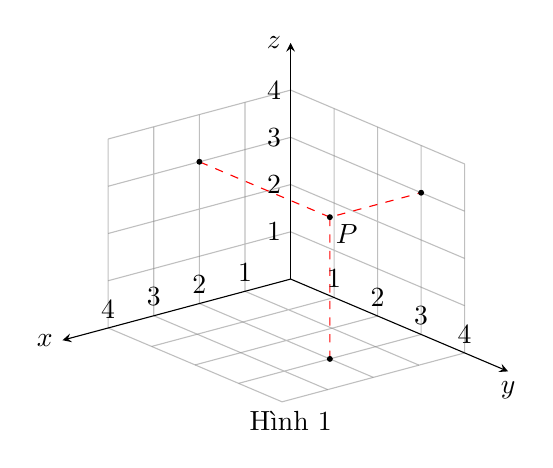
\begin{tikzpicture}[scale=.6]
			\def\goc{195}\def\a{2}\def\b{3}
			\path
			(0:0) coordinate (O)
			(-23:\b) coordinate (C)
			++(\goc:\a) coordinate (B)
			++(90:\b) coordinate (P)
			(\goc:\a) coordinate (A)
			(C)++(90:\b) coordinate (C')
			(90:\b) coordinate (O')
			++(\goc:\a) coordinate (A')
			;
			\foreach \x in {1,...,4}\draw[gray,opacity=.5] 
			(-23:\x) --++ (90:4) (90:\x)--++(-23:4)
			(0,\x)--++(\goc:4) (\goc:\x)--++(90:4)
			(\goc:\x)--++(-23:4) (-23:\x)--++(\goc:4)
			;
			\draw[-stealth] (O)--++(\goc:5) node[left]{$x$};
			\draw[-stealth] (O)--++(-23:5) node[below]{$y$};
			\draw[-stealth] (O)--++(90:5) node[left]{$z$};
			\draw[dashed,red]
			(B)--(P)--(C')
			(P)--(A')
			;
			\foreach \x/\g in {P/-45}\draw[fill=black] (\x) circle (.05) +(\g:.5) node{$\x$};
			\foreach \x in {A',B,C'}\draw[fill=black] (\x) circle (.05);
			\foreach \x in {1,...,4}\draw[black] (-23:\x) node[black,above]{\x};
			\foreach \x in {1,...,4}\draw[black] (\goc:\x) node[black,above]{\x};
			\foreach \x in {1,...,4}\draw[black] (90:\x) node[black,left]{\x};
			\draw (0,-3) node{Hình 1};
		\end{tikzpicture}
	}	
	\loigiai{
		Dựa vào hình vẽ, ta thấy điểm $P$ có tọa độ là $(2;3;3)$. \\
		$OP=\sqrt{2^2+3^2+3^2}=\sqrt{22}$.
	}
\end{bt}

% #1518 | Archive/2024/0. [LVH] BG - 12 New - 4in1-20240625T224301Z-001/0. [LVH] BG - 12 New - 4in1/data/data_C2/Bai-2-Dang3-ToaDoDiemDB.tex | mã gốc 2H2H2-2
\begin{bt}[Mức H]%[BG -12 New -4in1, Hector Tran]%[2H2H2-2]
	\immini{
		Trong không gian $O x y z$, cho hình hộp chữ nhật $O A B C . O' A' B' C'$ như Hình 2, biết $B'(2 ; 3 ; 5)$.
		\begin{enumerate}
			\item Tìm toạ độ các đỉnh còn lại của hình hộp.
			\item Tính độ dài đường chéo $O B'$ của hình hộp chữ nhật đó.
		\end{enumerate}
	}{
		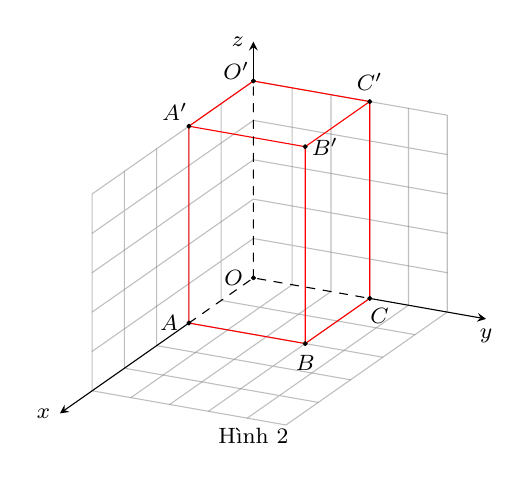
\begin{tikzpicture}[scale=.5, font=\footnotesize, line join=round, line cap=round, >=stealth]
			\def\goc{215}\def\a{2}\def\b{3}\def\c{5}
			\path
			(0:0) coordinate (O)
			(-10:\b) coordinate (C)
			++(\goc:\a) coordinate (B)
			++(90:\c) coordinate (B')
			(\goc:\a) coordinate (A)
			(C)++(90:\c) coordinate (C')
			(90:\c) coordinate (O')
			++(\goc:\a) coordinate (A')
			;
			\foreach \x in {1,...,5}\draw[gray,opacity=.5] 
			(-10:\x) --++ (90:5) (90:\x)--++(-10:5)
			(0,\x)--++(\goc:5) (\goc:\x)--++(90:5)
			(\goc:\x)--++(-10:5) (-10:\x)--++(\goc:5)
			;
			\draw[-stealth] (A)--++(\goc:4) node[left]{$x$};
			\draw[-stealth] (C)--++(-10:3) node[below]{$y$};
			\draw[-stealth] (O')--++(90:1) node[left]{$z$};
			\draw[red]
			(A)--(B)--(C)--(C')--(O')--(A')--cycle
			(A')--(B')--(B) (B')--(C')
			;
			\draw[dashed] (A)--(O)--(C) (O)--(O');
			\foreach \x/\g in {O/180,A/180,B/270,C/-60,A'/135,B'/0,O'/150,C'/90}\draw[fill=black] (\x) circle (.05) +(\g:.5) node{$\x$};
			\draw (0,-4) node{Hình 2};
		\end{tikzpicture}
	}	
	\loigiai{
		\begin{enumerate}
			\item Ta có 
			\begin{itemize}
				\item $O$ là gốc tọa độ nên $O(0;0;0)$;
				\item $B$ là hình chiếu vuông góc của $B'$ lên $(Oxy)$ nên $B(2;3;0)$;
				\item $C'$ là hình chiếu vuông góc của $B'$ lên $(Oyz)$ nên $A'(0;3;5)$;
				\item $A'$ là hình chiếu vuông góc của $B'$ lên $(Oxz)$ nên $A'(2;0;5)$;
				\item $A$ là hình chiếu vuông góc của $B'$ lên trục $Ox$ nên $A(2;0;0)$;
				\item $C$ là hình chiếu vuông góc của $B'$ lên trục $Oy$ nên $C(0;3;0)$;
				\item $O'$ là hình chiếu vuông góc của $B'$ lên trục $Oz$ nên $O'(0;0;5)$.
			\end{itemize}
			\item Ta có $OB'=\sqrt{2^2+3^2+5^2}=\sqrt{38}$.
		\end{enumerate}
	}
\end{bt}

% #1519 | Archive/2024/0. [LVH] BG - 12 New - 4in1-20240625T224301Z-001/0. [LVH] BG - 12 New - 4in1/data/data_C2/Bai-2-Dang3-ToaDoDiemDB.tex | mã gốc 2H2V2-2
\begin{bt}[Mức V]%[BG -12 New -4in1, Hector Tran]%[2H2V2-2]
	\immini{Cho hình chóp $S.ABC$ có đáy $ABC$ là tam giác đều cạnh bằng $2$, $SA$ vuông góc với đáy và $SA =1$. Thiết lập hệ toạ độ như hình vẽ bên, hãy vẽ các véc-tơ đơn vị trên các trục $Ox$, $Oy$, $Oz$ và tìm toạ độ các điểm $A$, $B$, $C$, $S$.
	}{
		\begin{tikzpicture}[scale=1, font=\footnotesize, line join=round, line cap=round, >=stealth]
			\path 
			(0:0) coordinate (A)
			++(0:4) coordinate (C)
			++(-160:3)coordinate(B)
			(A)++(90:2) coordinate (S)
			($(B)!1/2!(C)$) coordinate (O)
			($(S)+(O)-(A)$) coordinate (H)
			($(O)!1.4!(A)$) coordinate (y) node[above]{$y$}
			($(O)!1.4!(C)$) coordinate (x) node[above]{$x$}
			($(O)!1.4!(H)$) coordinate (z) node[right]{$z$}
			(intersection of S--C and O--H) coordinate (t)
			;
			\draw (S)--(A)--(B)--(C) (S)--(B) (O)--(z) (S)--(H) (C)--(t)
			;
			\draw[dashed] (C)--(A)--(O) (S)--(t)
			;
			\draw[->] (C)--(x); 
			\draw[->] (A)--(y);
			\draw[->] (H)--(z);
			\pic[draw,thin,angle radius=2mm] {right angle=S--A--O}
			pic[draw,thin,angle radius=2mm] {right angle=A--O--H}
			pic[draw,thin,angle radius=2mm] {right angle=O--H--S}
			pic[draw,thin,angle radius=2mm] {right angle=H--O--C}
			;
			\foreach \x/\g in {A/-100,C/-30,B/-90,O/-70,H/0,S/90}
			\fill (\x) circle (1pt)
			+(\g:3mm) node{$\x$};
		\end{tikzpicture}
	}	
	\loigiai{
		\immini{
			Vì $BC = 2$, $O$ là trung điểm $BC$ nên $OC =1$. Suy ra điểm cuối của véc-tơ $\overrightarrow{i}$ là điểm $C$.\\
			Vì $SAOH$ là hình chữ nhật nên $OH = SA = 1$. Suy ra điểm cuối của véc-tơ $\overrightarrow{k}$ là điểm $H$.\\ 
			Tam giác $ABC$ đều, có $AO$ là đường cao.\\
			Suy ra $AO = \sqrt{AB^2 - OB^2} = \sqrt{3}$. Trên cạnh $OA$, lấy điểm $j$ sao cho $Oj = 1$.\\
			Vậy ta được các véc-tơ $\overrightarrow{i}$, $\overrightarrow{j}$, $\overrightarrow{k}$ như hình vẽ.
		}{
			\begin{tikzpicture}[scale=1, font=\footnotesize, line join=round, line cap=round, >=stealth]
				\path 
				(0:0) coordinate (A)
				++(0:4) coordinate (C) node[below]{$\overrightarrow{i}$}
				++(-160:3)coordinate(B)
				(A)++(90:2) coordinate (S)
				($(B)!1/2!(C)$) coordinate (O)
				($(S)+(O)-(A)$) coordinate (H) node[right]{$\overrightarrow{k}$}
				($(O)!1.4!(A)$) coordinate (y) node[above]{$y$}
				($(O)!1.4!(C)$) coordinate (x) node[above]{$x$}
				($(O)!1.4!(H)$) coordinate (z) node[right]{$z$}
				($(O)!0.5!(A)$) coordinate (j) node[below]{$\overrightarrow{j}$}
				(intersection of S--C and O--H) coordinate (t)
				;
				\draw (S)--(A)--(B)--(C) (S)--(B) (O)--(z) (S)--(H) (C)--(t)
				;
				\draw[dashed] (C)--(A)--(O) (S)--(t)
				;
				\draw[->] (C)--(x); 
				\draw[->] (A)--(y);
				\draw[->] (H)--(z);
				\draw[->,red] (O)--(C); 
				\draw[->,red] (O)--(j);
				\draw[->,red] (O)--(H);
				\pic[draw,thin,angle radius=2mm] {right angle = S--A--O}
				pic[draw,thin,angle radius=2mm] {right angle = A--O--H}
				pic[draw,thin,angle radius=2mm] {right angle = O--H--S}
				pic[draw,thin,angle radius=2mm] {right angle = H--O--C}
				;
				\foreach \x/\g in {A/-100,C/90,B/-90,O/-70,H/140,S/90}
				\fill (\x) circle (1pt)
				+(\g:3mm) node{$\x$};
			\end{tikzpicture}
		}	
		Điểm $C$ nằm trên tia $Ox$, $OC = 1\Rightarrow \overrightarrow{OC} = 1\cdot \overrightarrow{i} + 0\cdot \overrightarrow{j} + 0\cdot \overrightarrow{k} \Rightarrow C(1; 0; 0)$.\\
		Điểm $B$ nằm trên tia đối của tia $Ox$, $OB = 1 \Rightarrow \overrightarrow{OB} = (-1)\cdot \overrightarrow{i} + 0\cdot \overrightarrow{j} + 0\cdot \overrightarrow{k} \Rightarrow B(-1; 0; 0)$.\\
		Điểm $A$ nằm trên tia $Oy$, $OA = \sqrt{3} \Rightarrow \overrightarrow{OA} = 0\cdot \overrightarrow{i} + \sqrt{3}\cdot \overrightarrow{j} + 0\cdot \overrightarrow{k}\Rightarrow A(0;\sqrt{3};0)$.\\
		Ta có $\overrightarrow{OS} = \overrightarrow{OA} + \overrightarrow{OH}  = 0\cdot \overrightarrow{i} + \sqrt{3}\cdot \overrightarrow{j} + 0\cdot \overrightarrow{k} + 0\cdot \overrightarrow{i} + 0\cdot \overrightarrow{j} + 1\cdot \overrightarrow{k} = 0\cdot \overrightarrow{i} + \sqrt{3}\cdot \overrightarrow{j} + 1\cdot \overrightarrow{k}$.\\
		Suy ra $S(0;\sqrt{3};1)$.
	}
\end{bt}

% #1528 | Archive/2024/0. [LVH] BG - 12 New - 4in1-20240625T224301Z-001/0. [LVH] BG - 12 New - 4in1/data/data_C2/Bai2-A-Phan-Ly-Thuyet.tex | mã gốc 2H2N2-1
\begin{vd}%[2H2N2-1]
		Cho tứ diện $OABC$ có $OA$, $OB$, $OC$ đôi một vuông góc và có độ dài bằng $1$. Vẽ hệ trục toạ độ $Oxyz$ có gốc là $O$, các điểm $A, B, C$ lần lượt nằm trên các tia $Ox$, $Oy$, $Oz$ và chỉ ra các véctơ đơn vị trên các trục toạ độ.
		\loigiai{
			\immini{
				Với $O$ là gốc toạ độ, ta vẽ được các trục $Ox$, $Oy$, $Oz$ như Hình bên. Ba véctơ đơn vị trên ba trục lần lượt là $\overrightarrow{i}=\overrightarrow{OA}$, $\overrightarrow{j}=\overrightarrow{OB}$, $\overrightarrow{k}=\overrightarrow{OC}$.
			}{
				\begin{tikzpicture}[scale=0.6, font=\footnotesize, line join=round, line cap=round, >=Stealth]
					\path 
					(0:0) coordinate (O)
					($(O)+(0:3)$) coordinate (B)
					($(O)+(90:3)$) coordinate (C)
					($(O)+(-155:2.5)$) coordinate (A)
					($(B)+(0:1)$) coordinate (y)
					($(C)+(90:1)$) coordinate (z)
					($(A)+(-155:1)$) coordinate (x)
					;
					\draw[->,dashed,red] (O)--(B) node[pos=.5,above]{$\overrightarrow{j}$};
					\draw[->,dashed,red] (O)--(C) node[pos=.5,left]{$\overrightarrow{k}$};
					\draw[->,dashed,red] (O)--(A) node[pos=.5,above=.1]{$\overrightarrow{i}$};
					\draw[->] (B)--(y) node[below]{$y$};
					\draw[->] (C)--(z) node[left]{$z$};
					\draw[->] (A)--(x) node[left]{$x$};
					\draw 	(A)--(B)--(C)--cycle
					pic[draw,angle radius=3mm]{right angle=B--O--C}
					pic[draw,angle radius=2mm]{right angle=C--O--A}
					pic[draw,angle radius=4mm]{right angle=A--O--B}
					;
					\foreach \x/\g in {O/45,B/-90,C/180,A/-80}
					\draw[fill=black] 	(\x) circle (.5pt)
					($(\g:.3)+(\x)$) node {$\x$};	
				\end{tikzpicture}
			}
		}
	\end{vd}

% #1530 | Archive/2024/0. [LVH] BG - 12 New - 4in1-20240625T224301Z-001/0. [LVH] BG - 12 New - 4in1/data/data_C2/Bai2-A-Phan-Ly-Thuyet.tex | mã gốc 2H2H2-3
\begin{vd}%[2H2H2-3]
				\immini{Trong không gian $Oxyz$, cho hình hộp chữ nhật $ABCD.A'B'C'D'$ có đỉnh $A$ trùng với gốc $O$, các véc-tơ $\overrightarrow{AB}$, $\overrightarrow{AD}$, $\overrightarrow{AA'}$ theo thứ tự cùng hướng với $\overrightarrow{i}, \overrightarrow{j}, \overrightarrow{k}$ và có $AB=8$, $AD=6$, $AA'=4$. Tìm toạ độ các véc-tơ $\overrightarrow{AB}$, $\overrightarrow{AC}$, $\overrightarrow{AC'}$ và $\overrightarrow{AM}$ với $M$ là trung điểm của cạnh $C'D'$.}{\begin{tikzpicture}[scale=0.6, font=\footnotesize, line join=round, line cap=round, >=Stealth]
						\path 
						(0:0) coordinate (B)
						($(B)+(-125:1)$) coordinate (x)
						(0:4) coordinate (C)
						($(B)+(55:4.3)$) coordinate (A)
						($(A)+(C)-(B)$) coordinate (D)
						($(D)+(0:1)$) coordinate (y)
						($(A)+(90:2.5)$) coordinate (A')
						($(A')+(90:1)$) coordinate (z)
						($(B)+(90:2.5)$) coordinate (B')
						($(C)+(90:2.5)$) coordinate (C')
						($(D)+(90:2.5)$) coordinate (D')
						($(A)!1/5!(B)$) coordinate (a)
						($(A)!1/3!(A')$) coordinate (o')
						($(A)!1/4!(D)$) coordinate (c)
						($(C')!.5!(D')$) coordinate (M)
						;
						\draw[dashed] (c)--(D) (a)--(B) (A')--(o') (A)--(C) (A)--(D');
						\draw[->,red] (A)--(a) node[right]{$\overrightarrow{i}$};
						\draw[->,red] (A)--(o') node[left=.1]{$\overrightarrow{k}$};
						\draw[->,red] (A)--(c) node[below]{$\overrightarrow{j}$};
						\draw[->] (A')--(z) node[left]{$z$};
						\draw[->] (D)--(y) node[below]{$y$};
						\draw[->] (B)--(x) node[right]{$x$};
						\draw 	(A')--(B')--(B)--(C)--(D) (B')--(C')--(C) (A')--(D')--(D) (D')--(C')
						;
						\foreach \x/\g in {A/170,B/180,C/0,D/-40,A'/180,B'/180,C'/0,D'/0,M/0}
						\draw[fill=black] 	(\x) circle (.5pt)
						($(\g:.3)+(\x)$) node {$\x$};	
				\end{tikzpicture}}
				\loigiai{
					Để tìm toạ độ của véctơ $\overrightarrow{AB}$, ta cần biểu diễn $\overrightarrow{AB}$ theo ba véctơ $\overrightarrow{i}, \overrightarrow{j}, \overrightarrow{k}$.\\
					Do $\overrightarrow{AB}$ cùng phương với $\overrightarrow{i}$ và $|\overrightarrow{AB}|=AB=8=8|\overrightarrow{i}|$ nên $\overrightarrow{AB}=8\overrightarrow{i}$ hay $\overrightarrow{AB}=8\overrightarrow{i}+0\overrightarrow{j}+0\overrightarrow{k}$.\\
					Tương tự, ta cũng có $\overrightarrow{AD}=0\overrightarrow{i}+6\overrightarrow{j}+0\overrightarrow{k}$, $\overrightarrow{AA'}=0\overrightarrow{i}+0\overrightarrow{j}+4\overrightarrow{k}$. \\
					Trong hình bình hành $ABCD$, ta có $\overrightarrow{AC}=\overrightarrow{AB}+\overrightarrow{AD}=8\overrightarrow{i}+6\overrightarrow{j}+0\overrightarrow{k}$.\\
					Trong hình bình hành $AA'C'C$, ta có $\overrightarrow{AC'}=\overrightarrow{AC}+\overrightarrow{AA'}=8\overrightarrow{i}+6\overrightarrow{j}+4\overrightarrow{k}$.\\
					Vì $M$ là trung điểm $C'D'$ nên $\begin{aligned}[t]
						\overrightarrow{AM}	&=\dfrac{1}{2}\left(\overrightarrow{AD'}+\overrightarrow{AC'}\right) \\
						&=\dfrac{1}{2}\left(\overrightarrow{AA'}+\overrightarrow{AD}+\overrightarrow{AC'}\right) \\
						&=\dfrac{1}{2}\left(4\overrightarrow{k}+6\overrightarrow{j}+8\overrightarrow{i}+6\overrightarrow{j}+4\overrightarrow{k}\right)\\
						&=4\overrightarrow{i}+6\overrightarrow{j}+4\overrightarrow{k}.
					\end{aligned}$
				}
			\end{vd}

% #1531 | Archive/2024/0. [LVH] BG - 12 New - 4in1-20240625T224301Z-001/0. [LVH] BG - 12 New - 4in1/data/data_C2/Bai-1-Dang-4-Gocgiuahaivecto.tex | mã gốc 2H2H1-3
\begin{vd}[CTST,Mức độ 2]%[Bài giảng-12,Mui Doan]%[2H2H1-3]
	Cho hình lập phương $ABCD.A'B'C'D'$. Xác định góc $\left(\overrightarrow{AB},\overrightarrow{A'D'}\right)$, $\left(\overrightarrow{AB},\overrightarrow{A'C'}\right)$.
	\loigiai{
		\immini{
			Ta có $\overrightarrow{AD}=\overrightarrow{A'D'}$, suy ra 
			$$\left(\overrightarrow{AB},\overrightarrow{A'D'}\right)=\left(\overrightarrow{AB},\overrightarrow{AD}\right)=\widehat{DAB}=90^{\circ}.$$
			Ta có $\overrightarrow{A'C'}=\overrightarrow{AC}$, suy ra 
			$$\left(\overrightarrow{AB},\overrightarrow{A'C'}\right)=\left(\overrightarrow{AB},\overrightarrow{AC}\right)=\widehat{BAC}=45^{\circ}.$$}
		{\vspace{-0.5cm}
			\begin{tikzpicture}[scale=0.7, font=\footnotesize, line join=round, line cap=round]
				\def\h{4}
				\foreach \x\y\t in {0/0/A',-1/-1.1/B',2.6/-1.1/C'}
				\coordinate (\t) at (\x,\y);
				\coordinate (D') at ($(A')+(C')-(B')$);
				\coordinate (A) at ($(A')+(0,3.2)$);
				\coordinate (B) at ($(B')+(0,3.2)$);
				\coordinate (C) at ($(C')+(0,3.2)$);
				\coordinate (D) at ($(D')+(0,3.2)$);
				\foreach \a\b in {A/B, A/D,A/C}
				\draw[-{Stealth[length=2mm]}] (\a)--(\b);
				\foreach \a\b in {A'/D',A'/C'}
				\draw[-{Stealth[length=2mm]},dashed] (\a)--(\b);
				\draw (D)--(C)--(B)--(B')--(C')--(D')--(D) (C')--(C);
				\draw[dashed](B')--(A')--(A);
				\foreach \t/\g in {A'/170,B'/-150,C'/-70,D'/0,A/100,B/170,C/-20,D/50}
				\draw[fill=black] (\t) circle(1pt)
				node[shift={(\g:7pt)}]{$\t$};
	\end{tikzpicture}}}
\end{vd}

% #1532 | Archive/2024/0. [LVH] BG - 12 New - 4in1-20240625T224301Z-001/0. [LVH] BG - 12 New - 4in1/data/data_C2/Bai-1-Dang-4-Gocgiuahaivecto.tex | mã gốc 2H2H1-3
\begin{vd}[CTST,Mức độ 2]%[Bài giảng-12,Mui Doan]%[2H2H1-3]
	Cho hình lập phương $ABCD.A'B'C'D'$. Xác định góc $\left(\overrightarrow{AC},\overrightarrow{B'D'}\right)$, $\left(\overrightarrow{A'A}, \overrightarrow{CB'}\right)$.
	\loigiai{
		\immini{
			Ta có $\overrightarrow{B'D'}=\overrightarrow{BD}$, suy ra\\
			$\left(\overrightarrow{AC},\overrightarrow{B'D'}\right)=\left(\overrightarrow{AC},\overrightarrow{BD}\right)=90^{\circ}$ (vì $\overrightarrow{AC} \perp \overrightarrow{BD}$).\\
			Ta có $\overrightarrow{B'B}=\overrightarrow{A'A}$, suy ra\\
			$\left(\overrightarrow{A'A},\overrightarrow{CB'}\right)=\left(\overrightarrow{B'B},\overrightarrow{CB'}\right)=180^{\circ}-\widehat{BB'C}=180^{\circ}-45^{\circ}=135^{\circ}$.}
		{\begin{tikzpicture}[scale=0.7, font=\footnotesize, line join=round, line cap=round]
				\def\h{4}
				\foreach \x\y\t in {0/0/A',-1/-1.1/B',2.6/-1.1/C'}
				\coordinate (\t) at (\x,\y);
				\coordinate (D') at ($(A')+(C')-(B')$);
				\coordinate (A) at ($(A')+(0,3.2)$);
				\coordinate (B) at ($(B')+(0,3.2)$);
				\coordinate (C) at ($(C')+(0,3.2)$);
				\coordinate (D) at ($(D')+(0,3.2)$);
				\foreach \a\b in {A/C, B/D,B'/B,C/B'}
				\draw[-{Stealth[length=2mm]}] (\a)--(\b);
				\foreach \a\b in {B'/D',A'/A}
				\draw[-{Stealth[length=2mm]},dashed] (\a)--(\b);
				\draw (B)--(A)--(D)--(C)--(B) (B')--(C')--(D')--(D) (C')--(C);
				\draw[dashed](B')--(A')--(D');
				\foreach \t/\g in {A'/170,B'/-150,C'/-70,D'/0,A/100,B/170,C/-20,D/50}
				\draw[fill=black] (\t) circle(1pt)
				node[shift={(\g:7pt)}]{$\t$};
		\end{tikzpicture}}
	}
\end{vd}

% #1533 | Archive/2024/0. [LVH] BG - 12 New - 4in1-20240625T224301Z-001/0. [LVH] BG - 12 New - 4in1/data/data_C2/Bai-1-Dang-4-Gocgiuahaivecto.tex | mã gốc 2H2H1-3
\begin{vd}[CD,Mức độ 2]%[Bài giảng-12,Mui Doan]%[2H2H1-3]
	Cho hình lập phương $ABCD.A'B'C'D'$ có cạnh bằng $a$.  Tính 
		các góc $\left( \vec{A'D},\vec{B'C'} \right)$; $\left(\vec{AD'},\vec{BD}\right)$.
	\loigiai{
		\immini
		{
		 Ta có $\left( \vec{A'D},\vec{B'C'} \right) = \left( \vec{A'D},\vec{A'D'} \right) = \widehat{DA'D'} = 45^\circ$.\\ 
		  $\left(\vec{AD'},\vec{BD}\right) = \left(\vec{BC'},\vec{BD}\right) = \widehat{C'BD}$.\\
		Do $BD = BC'=C'D= a\sqrt{2}$ nên tam giác $BDC'$ đều, từ đó suy ra $\left(\vec{AD'},\vec{BD}\right) = 60^\circ$.
		}
		{
			\begin{tikzpicture}[line join=round, line cap = round, >=stealth, scale=.8,font=\footnotesize,transform shape]
				\foreach \x/\y/\z/\g in
				{
					0/0/B/-135, 1.8/1/A/180, 4.8/1/D/0, 3/0/C/-45,
					0/3/B'/180, 1.8/4/A'/90, 4.8/4/D'/45, 3/3/C'/90
				}
				\draw[fill=black] (\x,\y) circle(1pt) coordinate (\z) ($(\z)+(\g:3.5mm)$) node{$\z$};
				\draw (C')--(D')--(C)--(C')--(B')--(A')--(D')--(D) (B')--(B)--(C)--(D);
				\draw[dashed] (B)--(A')--(A)--(B) (D')--(A)--(D);
			\end{tikzpicture}
		}		
	}
\end{vd}

% #1534 | Archive/2024/0. [LVH] BG - 12 New - 4in1-20240625T224301Z-001/0. [LVH] BG - 12 New - 4in1/data/data_C2/Bai-1-Dang-4-Gocgiuahaivecto.tex | mã gốc 2H2H1-3
\begin{vd}[KNTT,Mức độ 2]%[Bài giảng-12,Mui Doan]%[2H2H1-3]
	\immini{Cho hình lập phương $A B C D \cdot A' B' C' D'$ (hình bên).
		Tính góc giữa các cặp vectơ sau:
		\begin{enumerate}
			\item  $\overrightarrow{A D}$ và $\overrightarrow{B' C'}$;
			\item  $\overrightarrow{A C}$ và $\overrightarrow{A' D'}$.
	\end{enumerate}}{
		\begin{tikzpicture}[line join=round, line cap = round, >=stealth, scale=.7,font=\footnotesize,transform shape]
			\def\a{3.5}
			\path 	(0:0) coordinate (A)
			++(0:\a) coordinate (D)
			++(-130:\a/2) coordinate (C)
			($(A)+(C)-(D)$) coordinate (B)
			($(A)+(90:\a)$) coordinate (A')
			($(B)+(90:\a)$) coordinate (B')
			($(C)+(90:\a)$) coordinate (C')
			($(D)+(90:\a)$) coordinate (D');
			\draw[dashed] 	(B)--(A)	(A)--(A');
			\draw	(C)--(C') 		(B)--(B') 	(B)--(C)--(D) (A')--(B') (C')--(D')--(D);
			\foreach \x/\g in {A/180,B/180,C/0,D/0,A'/180,B'/180,C'/0,D'/0}
			\fill[black] 	(\x) circle (1pt)
			($(\g:4mm)+(\x)$) node {$\x$};	
			\draw[->] (B')--(C') (A')--(D');
			\draw[->,dashed] (A)--(D) (A)--(C);			
	\end{tikzpicture}	}	
	\loigiai{
		\begin{enumerate}
			\item  Hai vectơ $\overrightarrow{A D}$ và $\overrightarrow{B' C'}$ cùng hướng nên $\left(\overrightarrow{A D}, \overrightarrow{B' C'}\right)=0^{\circ}$.
			\item 	Vì tứ giác $A D D' A'$ là hình bình hành nên $\overrightarrow{A D}=\overrightarrow{A' D'}$.\\
			Do đó $\left(\overrightarrow{A C}, \overrightarrow{A' D'}\right)=(\overrightarrow{A C}, \overrightarrow{A D})=\widehat{C A D}$. \\
			Tam giác $A D C$ vuông cân tại $D$ nên $\widehat{C A D}=45^{\circ}$, vì vậy $\left(\overrightarrow{A C}, \overrightarrow{A' D'}\right)=45^{\circ}$.
	\end{enumerate}	}
\end{vd}

% #1535 | Archive/2024/0. [LVH] BG - 12 New - 4in1-20240625T224301Z-001/0. [LVH] BG - 12 New - 4in1/data/data_C2/Bai-1-Dang-5-Tichvohuongvaungdung.tex | mã gốc 2H2H1-3
\begin{vd}[Kết nối tri thức, Mức độ 2]%[BG - 12 New - 4in1, Paul Hieu Nguyen]%[2H2H1-3]
	\immini{ Cho tứ diện $A B C D$ có $A C$ và $B D$ cùng vuông góc với $A B$. Gọi $M, N$ lần lượt là trung điểm của hai cạnh $A B, C D$ (hình bên). Chứng minh rằng
		\begin{enumerate}[a)]
			\item   $\overrightarrow{M N}=\dfrac{1}{2}(\overrightarrow{A C}+\overrightarrow{B D})$;
			\item   $\overrightarrow{M N} \cdot \overrightarrow{A B}=0$.
	\end{enumerate}}{
		\begin{tikzpicture}[line join=round, line cap = round, >=stealth, scale=.8,font=\footnotesize,transform shape]
			\def\a{4}
			\path 	(0:0) coordinate (B)
			++(0:\a) coordinate (D)
			++(-120:\a/2) coordinate (C)
			($(B)+(70:\a)$) coordinate (A)
			($(A)!0.5!(B)$) coordinate (M)
			($(C)!0.5!(D)$) coordinate (N);
			\draw[dashed,thick] 	(B)--(D);
			\draw[thick] 			(B)--(A)--(D) (A)--(C)
			(B)--(C)--(D);
			\foreach \x/\g in {A/90,B/180,C/-45,D/0,M/120,N/-20}
			\fill[black] 	(\x) circle (1pt)
			($(\g:3mm)+(\x)$) node {$\x$};
			\draw[->,dashed] (M)--(N);		
			%Hình chóp S.ABC có SA vuông góc đáy	
	\end{tikzpicture}}	
	\loigiai{
		\begin{enumerate}[a)]
			\item  Ta có $\overrightarrow{M N}=\overrightarrow{M A}+\overrightarrow{A C}+\overrightarrow{C N}$ và $\overrightarrow{M N}=\overrightarrow{M B}+\overrightarrow{B D}+\overrightarrow{D N}$.\\
			Do đó $2 \overrightarrow{M N}=(\overrightarrow{M A}+\overrightarrow{M B})+(\overrightarrow{A C}+\overrightarrow{B D})+(\overrightarrow{C N}+\overrightarrow{D N})$.\\
			Vì $M, N$ lần lượt là trung điểm của $A B, C D$ nên $\overrightarrow{M A}+\overrightarrow{M B}=\overrightarrow{C N}+\overrightarrow{D N}=\overrightarrow{0}$.\\
			Suy ra $2 \overrightarrow{M N}=\overrightarrow{A C}+\overrightarrow{B D}$, hay $\overrightarrow{M N}=\dfrac{1}{2}(\overrightarrow{A C}+\overrightarrow{B D})$.
			\item 	Từ giả thiết, ta có $\overrightarrow{A C} \cdot \overrightarrow{A B}=\overrightarrow{B D} \cdot \overrightarrow{A B}=0$.\\
			Vì vậy, $\overrightarrow{M N} \cdot \overrightarrow{A B}=\dfrac{1}{2}(\overrightarrow{A C}+\overrightarrow{B D}) \cdot \overrightarrow{A B}=\dfrac{1}{2} \overrightarrow{A C} \cdot \overrightarrow{A B}+\dfrac{1}{2} \overrightarrow{B D} \cdot \overrightarrow{A B}=0$.
	\end{enumerate}	}
\end{vd}

% #1536 | Archive/2024/0. [LVH] BG - 12 New - 4in1-20240625T224301Z-001/0. [LVH] BG - 12 New - 4in1/data/data_C2/Bai-1-Dang-5-Tichvohuongvaungdung.tex | mã gốc 2H2H1-3
\begin{vd}[Chân trời sáng tạo, Mức độ 2]%[BG - 12 New - 4in1, Paul Hieu Nguyen]%[2H2H1-3]
	Cho tứ diện đều $ABCD$ có cạnh bằng $a$ và $M$ là trung điểm của $CD$.
	\begin{enumerate}
		\item Tính các tích vô hướng $\overrightarrow{AB} \cdot \overrightarrow{AC}$, $\overrightarrow{AB} \cdot \overrightarrow{AM}$.
		\item Tính góc $(\overrightarrow{AB}, \overrightarrow{CD})$.
	\end{enumerate}
	\loigiai{
		\immini{\begin{enumerate}
			\item Ta có $\begin{aligned}[t]
				\overrightarrow{AC}  \cdot \overrightarrow{AC}	&= \left|\overrightarrow{AB}\right| \cdot \left|\overrightarrow{AC}\right| \cdot \cos \left(\overrightarrow{AB},\overrightarrow{AC}\right)\\
				&= AB \cdot AC \cdot \cos \widehat{BAC}\\
				&= a \cdot a \cdot \cos {60^\circ}\\
				&= \frac{a^2}{2}.
			\end{aligned}$\\
			Tương tự ta cũng có $\overrightarrow{AB} \cdot \overrightarrow{AD}  = \dfrac{a^2}{2}$.\\
			Ta lại có $\overrightarrow{AM} = \dfrac{1}{2}(\overrightarrow{AC} + \overrightarrow{AD})$, suy ra
			$$ \overrightarrow{AB} \cdot \overrightarrow{AM} = \overrightarrow{AB} \cdot \frac{1}{2}(\overrightarrow{AC} +\overrightarrow{AD}) = \frac{1}{2}(\overrightarrow{AB} \cdot \overrightarrow{AC}  + \overrightarrow{AB}  \cdot \overrightarrow{AD}) = \frac{1}{2}\left(\frac{a^2}{2} + \frac{a^2}{2}\right) = \frac{a^2}{2}.$$
			\item Ta có $\overrightarrow{AB} \cdot \overrightarrow{CD}=(\overrightarrow{AM}+\overrightarrow{MB}) \cdot \overrightarrow{CD}=\overrightarrow{AM} \cdot \overrightarrow{CD} +\overrightarrow{MB} \cdot \overrightarrow{CD}$.\\
			Mà $AM$, $BM$ là trung tuyến của các tam giác đều $ACD$, $BCD$ nên\\ $\overrightarrow{AM}  \perp \overrightarrow{CD}$, $\overrightarrow{MB} \perp \overrightarrow{CD}$.\\
			Suy ra $\overrightarrow{AM} \cdot \overrightarrow{CD}  = \overrightarrow{MB} \cdot \overrightarrow{CD}  = 0$.\\
			Từ các kết quả trên ta có $\overrightarrow{AM} \cdot \overrightarrow{CD}=0$.
			Suy ra $(\overrightarrow{AB}, \overrightarrow{CD})=90^\circ$.
		\end{enumerate}
	}
	{
		\begin{tikzpicture}[scale=0.8, font=\footnotesize, line join=round, line cap=round, >=Stealth]
			\def\a{3}
			\path 
			(0:0) coordinate (B)
			(5:\a) coordinate (D)
			($(D)+(-135:\a/2)$) coordinate (C)
			($(B)+(65:\a)$) coordinate (A)
			($(C)!.5!(D)$) coordinate (M)
			;
			\draw[->] (A)--(D);
			\draw[->] (A)--(C);
			\draw[->] (A)--(B);
			\draw[->] (A)--(M);
			\draw[dashed] (B)--(D);
			\draw (B)--(C)--(D);
			\foreach \x/\g in {A/90,B/180,C/-90,D/0,M/0}
			\draw[fill=black] 	(\x) circle (.5pt)
			($(\g:.3)+(\x)$) node {$\x$};	
		\end{tikzpicture}
	}
	}
\end{vd}

% #1537 | Archive/2024/0. [LVH] BG - 12 New - 4in1-20240625T224301Z-001/0. [LVH] BG - 12 New - 4in1/data/data_C2/Bai-1-Dang-5-Tichvohuongvaungdung.tex | mã gốc 2H2H1-3
\begin{vd}[Cánh diều, Mức độ 2]%[BG - 12 New - 4in1, Paul Hieu Nguyen]%[2H2H1-3]
	Cho tứ diện $OABC$ có các cạnh $OA$, $OB$, $OC$ đôi một vuông góc và $OA = OB = OC = 1$. Gọi $M$ là trung điểm của cạnh $AB$. Tính góc giữa hai véc-tơ $\overrightarrow{OM}$ và $\overrightarrow{AC}$.
	\loigiai{
		\immini
		{
			Đặt $\overrightarrow{OA} = \overrightarrow{a}$, $\overrightarrow{OB} = \overrightarrow{b}$, $\overrightarrow{OC} = \overrightarrow{c}$.\\
			Khi đó, $|\overrightarrow{a}| = |\overrightarrow{b}| = |\overrightarrow{c}| = 1$ và $\overrightarrow{a} \cdot \overrightarrow{b} = \overrightarrow{b}\cdot \overrightarrow{c} = \overrightarrow{a}\cdot\overrightarrow{c} = 0$.\\
			Do $\overrightarrow{OM} = \dfrac{1}{2} \left( \overrightarrow{OA} + \overrightarrow{OB}\right) = \dfrac{1}{2}\left( \overrightarrow{a} + \overrightarrow{b} \right)$ và $\overrightarrow{AC} = \overrightarrow{OC} - \overrightarrow{OA} = \overrightarrow{c} - \overrightarrow{a}$ nên 
			\begin{eqnarray*}
				&\overrightarrow{OM}\cdot\overrightarrow{AC} &= \dfrac{1}{2}\left( \overrightarrow{a} + \overrightarrow{b} \right)\left(\overrightarrow{c} - \overrightarrow{a}\right)\\
				& & = \dfrac{1}{2} \left( \overrightarrow{a} \cdot \overrightarrow{c} - \overrightarrow{a}^2 + \overrightarrow{b}\cdot \overrightarrow{c} - \overrightarrow{b}\cdot\overrightarrow{a} \right) = -\dfrac{1}{2}.
			\end{eqnarray*}
		}
		{
			\begin{tikzpicture}[line join=round, line cap = round, >=stealth, scale=.8,font=\footnotesize,transform shape]
				\foreach \x/\y/\z/\g in
				{
					0/0/O/180, 0/2/C/90,1/-1/A/-90,3/1/B/0,2/0/M/-45
				}
				\draw[fill=black] (\x,\y) circle(1pt) coordinate (\z) ($(\z)+(\g:3.5mm)$) node{$\z$};
				\draw[->,dashed,color= blue] (O)--(M);
				\draw[->,color= blue] (A)--(C);
				\draw (A)--(B)--(C)--(O)--(A);
				\draw[dashed] (O)--(B);
			\end{tikzpicture}
		}
		\noindent Kết hợp với $\left|\overrightarrow{OM}\right| = OM = \dfrac{\sqrt{2}}{2}$ và $\left|\overrightarrow{AC}\right| = AC = \sqrt{2}$ suy ra
		$$
		\cos\left( \overrightarrow{OM},\overrightarrow{AC} \right) 
		= \dfrac{\overrightarrow{OM} \cdot \overrightarrow{AC}}{\left|\overrightarrow{OM}\right| \cdot \left|\overrightarrow{AC}\right|} = -\dfrac{1}{2}.
		$$
		Vậy $\left( \overrightarrow{OM},\overrightarrow{AC} \right) = 120^\circ$.
	}
\end{vd}

% #1538 | Archive/2024/0. [LVH] BG - 12 New - 4in1-20240625T224301Z-001/0. [LVH] BG - 12 New - 4in1/data/data_C2/Bai-1-Dang-5-Tichvohuongvaungdung.tex | mã gốc 2H2H1-3
\begin{vd}[Cùng khám phá, Mức độ 2]%[BG - 12 New - 4in1, Paul Hieu Nguyen]%[2H2H1-3]
	Cho hình chóp $S.ABC$ có $SA=SB=SC=AB=AC=a$ và $BC=a\sqrt2$. Tính góc giữa các véc-tơ $\overrightarrow{SC}$ và $\overrightarrow{AB}$
	\loigiai{
		\immini{
			Ta có
			\allowdisplaybreaks 
			\begin{eqnarray*}
				\cos \left(\overrightarrow{SC},\overrightarrow{AB}\right) &=& \dfrac{\overrightarrow{SC}\cdot \overrightarrow{AB}}{\left|\overrightarrow{SC}\right|\cdot \left|\overrightarrow{AB}\right|}\\
				&=& \dfrac{\left(\overrightarrow{SA}+\overrightarrow{AC}\right)\cdot \overrightarrow{AB}}{a^2}\\
				&=& \dfrac{\overrightarrow{SA}\cdot \overrightarrow{AB}+\overrightarrow{AC}\cdot \overrightarrow{AB}}{a^2}.
			\end{eqnarray*}
			Từ giả thiết suy ra $SAB$ là tam giác đều và $ABC$ là tam giác vuông cân tại $A$. Từ đó ta tính được
			\begin{center}
				$ \overrightarrow{SA}\cdot \overrightarrow{AB}=a\cdot a\cdot \cos 120^\circ=- \dfrac{a^2}{2}$ và $\overrightarrow{AC}\cdot \overrightarrow{AB}=0.$
			\end{center}
			Suy ra $\cos \left(\overrightarrow{SC},\overrightarrow{AB}\right)=- \dfrac{1}{2}$. Vậy $\left(\overrightarrow{SC},\overrightarrow{AB}\right)= 120^\circ$.
		}{
			\begin{tikzpicture}[line join=round, line cap = round, >=stealth, scale=0.8,font=\footnotesize]
				\path 
				(0,0) coordinate (A) 
				(5,0.2) coordinate (C) 
				(2,-1.5) coordinate (B) 
				(2.5,3.5) coordinate (S) 
				($(S)!1.3!(A)$) coordinate (M) 
				; 
				\draw[dashed] (A)--(C); 
				\draw (S)--(A)--(B)--(C)--(S)--(B) (A)--(M); 
				\draw pic[draw,angle eccentricity=1.2,angle radius=0.3cm]{right angle= B--A--C}
				pic[draw,angle eccentricity=1.2,angle radius=0.3cm]{angle= M--A--B};
				\foreach \x/\g in {S/90,A/165,B/-90,C/-90} \fill[black](\x) circle (1pt) ($(\x)+(\g:3mm)$)node{$\x$}; 
			\end{tikzpicture} 
		}
	}
\end{vd}

% #1539 | Archive/2024/0. [LVH] BG - 12 New - 4in1-20240625T224301Z-001/0. [LVH] BG - 12 New - 4in1/data/data_C2/Bai-1-Dang-5-Tichvohuongvaungdung.tex | mã gốc 2H2H1-3
\begin{vd}[Cùng khám phá, Mức độ 2]%[BG - 12 New - 4in1, Paul Hieu Nguyen]%[2H2H1-3]
	Cho tứ diện $ABCD$ có $DA=DB=a$, $BC= \dfrac{a}{2}$, $AB \perp BC$ và $\widehat{CBD}=45^\circ$. Tính góc giữa hai véc-tơ $\overrightarrow{AD}$ và $\overrightarrow{BC}$.
	\loigiai{
		\immini{
			Ta có
			\allowdisplaybreaks 
			\begin{eqnarray*}
				\cos \left(\overrightarrow{AD},\overrightarrow{BC}\right) &=& \dfrac{\overrightarrow{AD}\cdot \overrightarrow{BC}}{\left|\overrightarrow{AD}\right|\cdot \left|\overrightarrow{BC}\right|}\\
				&=& \dfrac{\left(\overrightarrow{AB}+\overrightarrow{BD}\right)\cdot \overrightarrow{BC}}{ \dfrac{a^2}{2} }\\
				&=& \dfrac{2\left(\overrightarrow{AB}\cdot \overrightarrow{BC}+\overrightarrow{BD}\cdot \overrightarrow{BC}\right)}{a^2}.
			\end{eqnarray*}
			Từ giả thiết ta tính được
			\begin{center}
				$ \overrightarrow{BD}\cdot \overrightarrow{BC}= \dfrac{a}{2} \cdot a\cdot \cos 45^\circ=\dfrac{a^2\sqrt2}{4}$ và $\overrightarrow{AB}\cdot \overrightarrow{BC}=0.$
			\end{center}
			Suy ra $\cos \left(\overrightarrow{AD},\overrightarrow{BC}\right)= \dfrac{\sqrt2}{2}$.\\ 
			Vậy $\left(\overrightarrow{AD},\overrightarrow{BC}\right)= 45^\circ$.
		}{
			\begin{tikzpicture}[line join=round, line cap = round, >=stealth, scale=0.8,font=\footnotesize]
				\path 
				(0,0) coordinate (B) 
				(5,0.2) coordinate (D) 
				(2,-1.5) coordinate (C) 
				(2.5,3.5) coordinate (A) 
				%($(S)!1.3!(A)$) coordinate (M) 
				; 
				\draw[dashed] (B)--(D); 
				\draw (A)--(B)--(C)--(D)--(A)--(C); 
				\draw pic[draw,angle eccentricity=1.2,angle radius=0.3cm]{right angle= A--B--C}
				pic[draw,angle eccentricity=1.2,angle radius=0.3cm]{angle= C--B--D};
				\foreach \x/\g in {A/90,B/165,C/-90,D/-90} \fill[black](\x) circle (1pt) ($(\x)+(\g:3mm)$)node{$\x$}; 
			\end{tikzpicture} 
		}
	}
\end{vd}

% #1546 | Archive/2024/0. [LVH] BG - 12 New - 4in1-20240625T224301Z-001/0. [LVH] BG - 12 New - 4in1/data/data_C2/Bai-1-Dang-5-Tichvohuongvaungdung.tex | mã gốc 2H2V1-3
\begin{bt}[Cùng khám phá, Mức độ 3]%[BG - 12 New - 4in1, Paul Hieu Nguyen]%[2H2V1-3]
	Cho tứ diện $ABCD$. Hai điểm $M$ và $N$ theo thứ tự là trung điểm của $AD$ và $BC$. Cho biết $AB = 10$, $CD = 6$, $MN = 7$.
	\begin{enumerate}
		\item Chứng minh rằng $\overrightarrow{MN}= \dfrac{1}{2} \left(\overrightarrow{AB}+ \overrightarrow{DC}\right)$.
		\item Từ kết quả câu a, hãy tính $\overrightarrow{AB}\cdot \overrightarrow{DC}$.
		\item Tính $\left(\overrightarrow{AB}, \overrightarrow{DC}\right)$.
	\end{enumerate}
	\loigiai{
		\immini{\begin{enumerate}
			\item Ta có
			\allowdisplaybreaks 
			\begin{eqnarray*}
				\overrightarrow{MN} &=& \overrightarrow{MA}+ \overrightarrow{AB}+ \overrightarrow{BN}\\
				\overrightarrow{MN} &=& \overrightarrow{MD}+ \overrightarrow{DC}+ \overrightarrow{CN}.
			\end{eqnarray*}
			Do đó $2 \overrightarrow{MN}= \overrightarrow{AB}+ \overrightarrow{DC} \Rightarrow \overrightarrow{MN}= \dfrac{1}{2} \left(\overrightarrow{AB}+ \overrightarrow{DC}\right)$.
			\item Theo câu a) $2 \overrightarrow{MN}= \overrightarrow{AB}+ \overrightarrow{DC}$, do đó
			\allowdisplaybreaks 
			\begin{eqnarray*}
				4MN^2 &=& \left(\overrightarrow{AB}+ \overrightarrow{DC}\right)^2\\
				&=& \overrightarrow{AB}^2+ \overrightarrow{DC}^2+ 2\overrightarrow{AB}\cdot \overrightarrow{DC}\\
				\Rightarrow 4\cdot 7^2 &=& 10^2+6^2+2\overrightarrow{AB}\cdot \overrightarrow{DC}\\
				\Rightarrow \overrightarrow{AB}\cdot \overrightarrow{DC} &=& 30.
			\end{eqnarray*}
			\item Theo câu b) ta có
			\allowdisplaybreaks 
			\begin{eqnarray*}
				30 &=& \overrightarrow{AB}\cdot \overrightarrow{DC}\\
				&=& AB\cdot DC\cdot\cos \left(\overrightarrow{AB}, \overrightarrow{DC}\right)\\
				&=& 60 \cdot\cos \left(\overrightarrow{AB}, \overrightarrow{DC}\right)\\
				\Rightarrow \cos \left(\overrightarrow{AB}, \overrightarrow{DC}\right) &=& \dfrac{1}{2}\\
				\Rightarrow \left(\overrightarrow{AB}, \overrightarrow{DC}\right) &=& 60^\circ.
			\end{eqnarray*}
		\end{enumerate}
		}
	{
		\begin{tikzpicture}[line join=round, line cap = round, >=stealth, scale=0.9,font=\footnotesize]
			\path  
			(0,0) coordinate (B) 
			(5,0.2) coordinate (D) 
			(2,-1.5) coordinate (C) 
			(2.5,3.5) coordinate (A) 
			($(C)!1/2!(B)$) coordinate (N) 
			($(A)!1/2!(D)$) coordinate (M)
			; 
			\draw[dashed] (B)--(D) (M)--(N); 
			\draw (A)--(B)--(C)--(D)--(A)--(C); 
			\foreach \x/\g in {A/90,B/165,C/-90,D/-90,M/40,N/-140} \fill[black](\x) circle (1pt) ($(\x)+(\g:3mm)$)node{$\x$}; 
		\end{tikzpicture}
	}
	}
\end{bt}

% #1547 | Archive/2024/0. [LVH] BG - 12 New - 4in1-20240625T224301Z-001/0. [LVH] BG - 12 New - 4in1/data/data_C2/Bai-1-Dang-5-Tichvohuongvaungdung.tex | mã gốc 2H2V1-3
\begin{bt}[Kết nối tri thức, Mức độ 3]%[BG - 12 New - 4in1, Paul Hieu Nguyen]%[2H2V1-3]
	Cho tứ diện $A B C D$. Chứng minh rằng
	\begin{enumerate}[a)]	
		\item   $\overrightarrow{A B} \cdot \overrightarrow{C D}=\overrightarrow{A C} \cdot \overrightarrow{C D}+\overrightarrow{B C} \cdot \overrightarrow{D C}$;
		\item  $\overrightarrow{A B} \cdot \overrightarrow{C D}+\overrightarrow{A C} \cdot \overrightarrow{D B}+\overrightarrow{A D} \cdot \overrightarrow{B C}=0$.	
	\end{enumerate}
	\loigiai{
		\immini{\begin{enumerate}[a)]	
				\item   Ta có $\overrightarrow{A C} \cdot \overrightarrow{C D}+\overrightarrow{B C} \cdot \overrightarrow{D C}= \overrightarrow{C D}\left(\overrightarrow{A C} -\overrightarrow{B C}  \right)=\overrightarrow{A B} \cdot \overrightarrow{C D} $;
				\item  Ta có
				\begin{eqnarray*}
					&&\overrightarrow{A B} \cdot \overrightarrow{C D}+\overrightarrow{A C} \cdot \overrightarrow{D B}+\overrightarrow{A D} \cdot \overrightarrow{B C}\\
					&=&\left(\overrightarrow{AC}+\overrightarrow{CB}\right) \cdot \overrightarrow{C D}+\overrightarrow{A C} \cdot \overrightarrow{D B}+\overrightarrow{A D} \cdot \overrightarrow{B C}\\
					&= & \overrightarrow{A C} \cdot \overrightarrow{C D}+\overrightarrow{B C} \cdot \overrightarrow{D C}+\overrightarrow{A C} \cdot \overrightarrow{D B}+\overrightarrow{A D} \cdot \overrightarrow{B C}\\
					&=& \overrightarrow{A C} \cdot \left(\overrightarrow{C D} +\overrightarrow{D B}\right)+\overrightarrow{B C}\cdot\left(\overrightarrow{A D}+\overrightarrow{DC} \right)\\
					&=& \overrightarrow{A C} \cdot \overrightarrow{CB} +\overrightarrow{BC} \cdot\overrightarrow{AC}=0.
				\end{eqnarray*}
		\end{enumerate}}{\begin{tikzpicture}[font=\footnotesize,line join=round, line cap=round, >=stealth,scale=0.7] 
				\def\a{4}
				\path 	(0:0) coordinate (B)
				++(0:\a) coordinate (D)
				++(-120:\a/2) coordinate (C)
				($(B)+(70:\a)$) coordinate (A);
				\draw[dashed,thick] 	(B)--(D);
				\draw[thick] 			(B)--(A)--(D) (A)--(C)
				(B)--(C)--(D);
				\foreach \x/\g in {A/90,B/180,C/-45,D/0}
				\fill[black] 	(\x) circle (1pt)
				($(\g:3mm)+(\x)$) node {$\x$};
				%Hình chóp S.ABC có SA vuông góc đáy	
		\end{tikzpicture}}		
	}
\end{bt}

% #1548 | Archive/2024/0. [LVH] BG - 12 New - 4in1-20240625T224301Z-001/0. [LVH] BG - 12 New - 4in1/data/data_C2/Bai-1-Dang-5-Tichvohuongvaungdung.tex | mã gốc 2H2V1-3
\begin{bt}[Cánh diều, Mức độ 3]%[BG - 12 New - 4in1, Paul Hieu Nguyen]%[2H2V1-3]
	Cho hình lập phương $ABCD.A'B'C'D'$ có cạnh bằng $a$. Tính 
	$\overrightarrow{A'B}\cdot \overrightarrow{D'C'}$; $\overrightarrow{D'A} \cdot \overrightarrow{BC}$.
	\loigiai{
		\immini
		{
			Ta có 
				\begin{itemize}
					\item $\overrightarrow{A'B}\cdot \overrightarrow{D'C'} 
					= \overrightarrow{D'C} \cdot \overrightarrow{D'C'} 
					= D'C\cdot D'C' \cdot \cos 45^\circ
					= a\sqrt{2} \cdot a \cdot \dfrac{1}{\sqrt{2}} = a^2$.
					\item $\overrightarrow{D'A} \cdot \overrightarrow{BC} 
					= -\overrightarrow{AD'} \cdot \overrightarrow{AD} 
					= - AD'\cdot AD\cdot \cos 45^\circ
					= - a\sqrt{2} \cdot a \cdot \dfrac{1}{\sqrt{2}} = -a^2 $.
				\end{itemize}
		}
		{
			\begin{tikzpicture}[line join=round, line cap = round, >=stealth, scale=.7,font=\footnotesize,transform shape]
				\foreach \x/\y/\z/\g in
				{
					0/0/B/-135, 1.8/1/A/160, 4.8/1/D/0, 3/0/C/-45,
					0/3/B'/180, 1.8/4/A'/90, 4.8/4/D'/45, 3/3/C'/90
				}
				\draw[fill=black] (\x,\y) circle(1pt) coordinate (\z) ($(\z)+(\g:3.5mm)$) node{$\z$};
				\draw (C')--(D')--(C)--(C')--(B')--(A')--(D')--(D) (B')--(B)--(C)--(D);
				\draw[dashed] (B)--(A')--(A)--(B) (D')--(A)--(D);
			\end{tikzpicture}
		}
	}
\end{bt}

% #1549 | Archive/2024/0. [LVH] BG - 12 New - 4in1-20240625T224301Z-001/0. [LVH] BG - 12 New - 4in1/data/data_C2/Bai-1-Dang-5-Tichvohuongvaungdung.tex | mã gốc 2H2V1-3
\begin{bt}[Mức độ 3]%[BG - 12 New - 4in1, Paul Hieu Nguyen]%[2H2V1-3]
	Cho hình lăng trụ $ABC.A'B'C'$ có đáy $ABC$ là tam giác đều cạnh $a$, tam giác $A'BC$ đều nằm trong mặt phẳng vuông góc với $\left(ABC\right)$. Gọi $M$ là trung điểm cạnh $CC'$. Tính $\overrightarrow{AA'}\cdot\overrightarrow{BM}$.
	\loigiai{
		\immini{Ta có $AH=A'H=\dfrac{a\sqrt 3}{2}$ và $AH\perp BC,A'H\perp BC$ $\Rightarrow BC\perp\left(AA'H\right)$\\
		$\Rightarrow BC\perp AA'$ hay $BC\perp BB'$.\\
		Do đó $BCC'B'$ là hình chữ nhật.\\
		Khi đó $CC'=AA'=\dfrac{a\sqrt 3}{2}\cdot\sqrt 2=\dfrac{a\sqrt 6}{2}$ $\Rightarrow BM=\sqrt{a^2+\dfrac{a^2\cdot6}{16}}=a\cdot\dfrac{\sqrt{22}}{4}$.\\
		Do đó $\overrightarrow{AA'}\cdot\overrightarrow{BM}=\overrightarrow{AA'}\cdot\left(\overrightarrow{BC}+\overrightarrow{CM}\right)=0+AA'\cdot CM =\dfrac{3a^2}{4}$.
	}
	{
		\begin{tikzpicture}[>=stealth,line join=round,line cap=round,font=\footnotesize,scale=1]
			\tikzset{declare function={a=2;b=1.2;h=2.7;goc=-45;}}
			\coordinate (A) at (0,0);
			\coordinate (C) at (a,0);
			\coordinate (B) at (goc:b);
			\coordinate (H) at ($(C)!.5!(B)$);
			\coordinate (A') at ($(H)+(0,h)$);
			\coordinate (B') at ($(B)+(A')-(A)$);
			\coordinate (C') at ($(C)+(A')-(A)$);
			\coordinate (M) at ($(C)!.5!(C')$);
			\draw (B)--(A')--(A)--(B)--(C)--(C')--(A')--(B')--(B)--(M) (B')--(C');
			\draw[dashed] (A)--(C)--(A')--(H)--(A);
			\foreach \d/\g in {A/180,B/-90,C/0,A'/150,B'/-25,C'/20,H/-80,M/0}
			\fill[black](\d) circle (1pt)+(\g:.25)node[scale=.85]{$\d$};
		\end{tikzpicture}
	}
	}
\end{bt}

% #1550 | Archive/2024/0. [LVH] BG - 12 New - 4in1-20240625T224301Z-001/0. [LVH] BG - 12 New - 4in1/data/data_C2/Bai-1-Dang-5-Tichvohuongvaungdung.tex | mã gốc 2H2V1-3
\begin{bt}[Mức độ 3]%[BG - 12 New - 4in1, Paul Hieu Nguyen]%[2H2V1-3]
	Cho hình chóp $S.ABCD$ có tất cả các cạnh bên và cạnh đáy đều bằng $a$ và $ABCD$ là hình vuông. Gọi $M$ là trung điểm của $CD$. Tính $\overrightarrow{MS}.\overrightarrow{CB}$.
	\loigiai{
		\immini{Do tất cả các cạnh của hình chóp bằng nhau nên hình chóp $S.ABCD$ là hình chóp đều $\Rightarrow\left\{\begin{array}{l}
			SO\perp (ABCD)\\
			AC\perp BD
		\end{array}\right.$.\\
		Do $M$ là trung điểm của CD nên ta có\\
		$\overrightarrow{MS}=\overrightarrow{OS}-\overrightarrow{OM}
		=-\dfrac{1}{2}\overrightarrow{OC}-\dfrac{1}{2}\overrightarrow{OD}+\overrightarrow{OS}$,\\
		$\overrightarrow{CB}=\overrightarrow{OB}-\overrightarrow{OC}
		=-\overrightarrow{OD}-\overrightarrow{OC}$.\\
		Do $\overrightarrow{OC}$, $\overrightarrow{OS}$, $\overrightarrow{OD}$ đôi một vuông góc với nhau nên ta có\\
		$\overrightarrow{MS}\cdot\overrightarrow{CB}=\dfrac{1}{2}OC^2+\dfrac{1}{2}OD^2=OC^2=\dfrac{a^2}{2}$.
	}
{
		\begin{tikzpicture}[>=stealth,line join=round,line cap=round,font=\footnotesize,scale=1]
			\tikzset{declare function={a=2.2;b=1.3;h=1.7;goc=-140;}}
			\coordinate (A) at (0:0);
			\coordinate (D) at (0:a);
			\coordinate (B) at (goc:b);
			\coordinate (C) at ($(B)+(D)-(A)$);
			\coordinate (O) at ($(A)!.5!(C)$);
			\coordinate (S) at ($(O)+(0,h)$);
			\coordinate (M) at ($(C)!.5!(D)$);
			\draw (M)--(S)--(B)--(C)--(D)--(S)--(C);
			\draw[dashed] (B)--(A)--(D)--(B) (M)--(O)--(S)--(A)--(C);
			\foreach \d/\g in {A/140,B/200,C/-60,D/0,S/90,O/-105,M/0}
			\fill[black](\d) circle (1pt)+(\g:.2)node[scale=.85]{$\d$};
		\end{tikzpicture}
}
	}
\end{bt}

% #1561 | Archive/2024/0. [LVH] BG - 12 New - 4in1-20240625T224301Z-001/0. [LVH] BG - 12 New - 4in1/data/data_C2/Bai-3-Dang-1-Timtoadovectotong.tex | mã gốc 2H2N2-3
\begin{vd}%[Cánh diều]%[BG12 New, Anh Duy]%[2H2N2-3]
	Cho $\vec{a}=(-2;3;2)$, $\vec{b}=(2;1;-1)$, $\vec{c}=(1;2;3)$. Tính tọa độ của mỗi véc-tơ sau
	\begin{enumEX}{3}
		\item $3\vec{a}$; 
		\item $2\vec{a}-\vec{b}$;
		\item $\vec{a}+2\vec{b}-\dfrac{3}{2}\vec{c}$.
	\end{enumEX}
	\loigiai{
		\begin{enumerate}[a)]
			\item Ta có $3\vec{a}=(3\cdot (-2);3\cdot 3;3\cdot 2)$. Vậy $3\vec{a}=(-6;9;6)$.
			\item Ta có $2\vec{a}=(-4;6;4)$ và $\vec{b}=(2;1;-1)$.\\
			Do đó, $2\vec{a}-\vec{b}=(-4-2;6-1;4-(-1))$.\\
			Vậy $2\vec{a}-\vec{b}=(-6;5;5)$.
			\item Do $\vec{a}=(-2;3;2)$ và $2\vec{b}=(4;2;-1)$ nên $\vec{a}+2\vec{b}=(2;5;0)$.\\
			Ngoài ra, vì $-\dfrac{3}{2}\vec{c}=\left(-\dfrac{3}{2};-3;-\dfrac{9}{2}\right)$ nên $\vec{a}+2\vec{b}-\dfrac{3}{2}\vec{c}=\left(\dfrac{1}{2};2;-\dfrac{9}{2}\right)$.
		\end{enumerate}
	}
\end{vd}

% #1562 | Archive/2024/0. [LVH] BG - 12 New - 4in1-20240625T224301Z-001/0. [LVH] BG - 12 New - 4in1/data/data_C2/Bai-3-Dang-1-Timtoadovectotong.tex | mã gốc 2H2H2-3
\begin{vd}%[Cánh diều]%[BG12 New, Anh Duy]%[2H2H2-3]
	Cho ba điểm $A(0;-1;1)$, $B(1;0;5)$, $G(1;2;0)$.
	\begin{enumerate}
		\item Chứng minh rằng ba điểm $A$, $B$, $G$ không thẳng hàng.
		\item Tìm tọa độ điểm $C$ sao cho $G$ là trọng tâm của tam giác $ABC$.
	\end{enumerate}
	\loigiai{
		\begin{enumerate}
			\item Ta có $\vec{AB}=(1;1;4)$ và $\vec{AG}=(1;3;-1)$.\\
			Suy ra $\vec{AB}\ne k\vec{AG}$ với mọi $k\in \mathbb{R}$.\\
			Suy ra $\vec{AB}$, $\vec{AG}$ không cùng phương.\\
			Vậy $A$, $B$, $G$ không thẳng hàng.
			\item Ta có $G$ là trọng tâm tam giác $ABC$ nên
			$$\heva{&1=\dfrac{0+1+x_C}{3}\\&2=\dfrac{-1+0+y_C}{3}\\&0=\dfrac{1+5+z_C}{3}}\Rightarrow \heva{&x_C=2\\&y_C=7\\&z_C=-6} \Rightarrow C(2;7;-6).$$
		\end{enumerate}
	}
\end{vd}

% #1563 | Archive/2024/0. [LVH] BG - 12 New - 4in1-20240625T224301Z-001/0. [LVH] BG - 12 New - 4in1/data/data_C2/Bai-3-Dang-1-Timtoadovectotong.tex | mã gốc 2H2H2-3
\begin{vd}%[CTST]%[BG12 New, Anh Duy]%[2H2H2-3]
	Cho các điểm $A(-1 ;-1 ; 0)$, $B(0 ; 3 ;-1)$, $C(-1 ; 14 ; 0)$, $D(-3 ; 6 ; 2)$. Chứng minh rằng $A B C D$ là hình thang.
	\loigiai{
		Ta có $\overrightarrow{AB}=(1;4;-1)$, $\overrightarrow{BC}=(-1;11;1)$, $\overrightarrow{CD}=(-2,-8,2)$.\\
		Do $\overrightarrow{CD}=(-2)\cdot \overrightarrow{AB}$ nên hai véctơ $\overrightarrow{CD}$ và $\overrightarrow{AB}$ ngược hướng với nhau, suy ra hai đường thẳng $AB$ và $CD$ hoặc là song song, hoặc là trùng nhau.\\
		Mặt khác ta lại có hai véctơ $\overrightarrow{AB}$ và $\overrightarrow{BC}$ không cùng phương nên ba điểm $A$, $B$, $C$ không thẳng hàng. Vậy $ABCD$ là hình thang. 
	}
\end{vd}

% #1565 | Archive/2024/0. [LVH] BG - 12 New - 4in1-20240625T224301Z-001/0. [LVH] BG - 12 New - 4in1/data/data_C2/Bai-3-Dang-1-Timtoadovectotong.tex | mã gốc 2H2H2-3
\begin{vd}%[BG12 New, Anh Duy]%[2H2H2-3]
	\immini{
		Cho hình chóp $S.ABC$ có $SA \perp (ABC)$, $SA = a$ và đáy $ABC$ là tam giác đều cạnh $a$, $O$ là trung điểm của $BC$. Bằng cách thiết lập hệ toạ độ như hình vẽ, hãy tìm toạ độ
		\begin{enumerate}
			\item Các điểm $A$, $S$, $B$, $C$;
			\item Trung điểm $M$ của $SB$ và trung điểm $N$ của $SC$;
			\item Trọng tâm $G$ của tam giác $SBC$.
		\end{enumerate}
	}{
		\begin{tikzpicture}[join = round, cap = round, thick, font = \footnotesize, scale =.5]
			\path 
			(0:0) coordinate (A)
			++(0:4) coordinate (C)
			++(-160:3)coordinate(B)
			(A)++(90:2) coordinate (S)
			($(B)!1/2!(C)$) coordinate (O)
			($(S)+(O)-(A)$) coordinate (H)
			($(O)!1.4!(A)$) coordinate (y) node[above]{$y$}
			($(O)!1.4!(C)$) coordinate (x) node[above]{$x$}
			($(O)!1.4!(H)$) coordinate (z) node[right]{$z$}
			(intersection of S--C and O--H) coordinate (t)
			;
			\draw (S)--(A)--(B)--(C) (S)--(B) (O)--(z) (S)--(H) (C)--(t)
			;
			\draw[dashed] (C)--(A)--(O) (S)--(t)
			;
			\draw[->] (C)--(x); 
			\draw[->] (A)--(y);
			\draw[->] (H)--(z);
			\draw 
			pic[draw,thin,angle radius=2mm] {right angle = S--A--O}
			pic[draw,thin,angle radius=2mm] {right angle = A--O--H}
			pic[draw,thin,angle radius=2mm] {right angle = O--H--S}
			pic[draw,thin,angle radius=2mm] {right angle = H--O--C}
			;
			\foreach \x/\g in {A/-100,C/-30,B/-90,O/-70,H/0,S/90}
			\fill (\x) circle (1pt)
			+(\g:3mm) node{$\x$};
		\end{tikzpicture}
	}
	\loigiai{
		\begin{enumerate}
			\item Với hệ trục tọa độ trên ta có 
			\[ C\left(\dfrac{a}{2}; 0; 0\right), B\left(-\dfrac{a}{2}; 0; 0\right), A\left(0; \dfrac{a\sqrt{3}}{2}; 0\right), S\left(0; \dfrac{a\sqrt{3}}{2}; a\right). \]
			\item Tọa độ trung điểm của $SB$, $SC$ là $M\left(-\dfrac{a}{4}; \dfrac{a\sqrt{3}}{4};\dfrac{a}{2}\right)$, $N\left(\dfrac{a}{4}; \dfrac{a\sqrt{3}}{4};\dfrac{a}{2}\right)$.
			\item Tọa độ trọng tâm $G$ của tam giác $ABC$ là  $G\left(0; \dfrac{a\sqrt{3}}{6};\dfrac{a}{3}\right)$.
		\end{enumerate}
	}
\end{vd}

% #1566 | Archive/2024/0. [LVH] BG - 12 New - 4in1-20240625T224301Z-001/0. [LVH] BG - 12 New - 4in1/data/data_C2/Bai-3-Dang-1-Timtoadovectotong.tex | mã gốc 2H2H2-3
\begin{bt}%[BG12 New, Anh Duy]%[2H2H2-3]
	Trong không gian với hệ tọa độ $Oxyz$, cho $\vec{a}=(-1;2;3)$, $\vec{b}=(3;1;-2)$, $\vec{c}=(4;2;-3)$.
	\begin{enumerate}
		\item Tìm tọa độ của véc-tơ $\vec{u}=2\vec{a}+\vec{b}-3\vec{c}$.
		\item Tìm tọa độ của véc-tơ $\vec{v}$ sao cho $\vec{v}+2\vec{b}=\vec{a}+\vec{c}$.
	\end{enumerate}
	\loigiai{
		\begin{enumerate}
			\item Ta có $2\vec{a}=(-2;4;6)$,  $3\vec{c}=(12;6;-9)$.\\
			Suy ra $\vec{u}=2\vec{a}+\vec{b}-3\vec{c}=(-11;-1;13)$.
			\item Ta có $2\vec{b}=(6;2;-4)$.\\
			Khi đó $\vec{v}=\vec{a}+\vec{c}-2\vec{b}=(-3;2;4)$.
		\end{enumerate}
	}
\end{bt}

% #1567 | Archive/2024/0. [LVH] BG - 12 New - 4in1-20240625T224301Z-001/0. [LVH] BG - 12 New - 4in1/data/data_C2/Bai-3-Dang-1-Timtoadovectotong.tex | mã gốc 2H2H2-3
\begin{bt}%[BG12 New, Anh Duy]%[2H2H2-3]
	Trong không gian $Oxyz$, cho bốn điểm $A(0;1;-2)$, $B(2;-1;3)$, $C(1;3;-2)$, $D(5;-1;8)$.
	\begin{enumerate}
		\item Ba điểm $A$, $B$, $C$ có thẳng hàng không ?
		\item Chứng minh rằng hai đường thẳng $AB$ và $CD$ song song nhau.
	\end{enumerate}
	\loigiai{
		\begin{enumerate}
			\item Ta có $\overrightarrow{AB}=(2;-2;5)$ và $\overrightarrow{AC}=(1;2;0)$. Do $\overrightarrow{AB}\neq k\overrightarrow{AC}$, với mọi $k$ nên $\overrightarrow{AB}$ và $\overrightarrow{AC}$ không cùng phương. Suy ra $A$, $B$, $C$ không thẳng hàng.
			\item Ta có $\overrightarrow{CD}=(4;-4;10)$ và $\overrightarrow{AB}=(2;-2;5)$ nên $\overrightarrow{CD}=2\overrightarrow{AB}$ mà $A$, $B$, $C$ không thẳng hàng nên $AB$ và $CD$ song song nhau.
		\end{enumerate}
	}
\end{bt}

% #1568 | Archive/2024/0. [LVH] BG - 12 New - 4in1-20240625T224301Z-001/0. [LVH] BG - 12 New - 4in1/data/data_C2/Bai-3-Dang-1-Timtoadovectotong.tex | mã gốc 2H2H2-3
\begin{bt}%[BG12 New, Anh Duy]%[2H2H2-3]
	Trong không gian $Oxyz$, cho ba điểm $A(1;3;-5)$, $M\left(\dfrac{3}{2};2;\dfrac{1}{2}\right)$, $G\left(2;\dfrac{2}{3};-\dfrac{2}{3}\right)$.
	\begin{enumerate}
		\item Tìm tọa độ điểm $B$ sao cho $M$ là trung điểm $AB$.
		\item Tìm tọa độ điểm $C$ sao cho $G$ là trọng tâm tam giác $ABC$.
	\end{enumerate}
	\loigiai{
		\begin{enumerate}
			\item $M$ là trung điểm $AB$ nên $2\overrightarrow{OM}=\overrightarrow{OA}+\overrightarrow{OB}\Rightarrow \overrightarrow{OB}=2\overrightarrow{OM}-\overrightarrow{OA}=(2;1;6)$, do đó $B(2;1;6)$.
			\item $G$ là trọng tâm tam giác $ABC$ nên $$3\overrightarrow{CG}=2\overrightarrow{CM}\Leftrightarrow 3\left(\overrightarrow{OG}-\overrightarrow{OC}\right)=2\left(\overrightarrow{OM}-\overrightarrow{OC}\right)\Leftrightarrow \overrightarrow{OC}=3\overrightarrow{OG}-2\overrightarrow{OM}\Leftrightarrow\overrightarrow{OC}=(3;-2;-3)$$
			Vậy $C(3;-2;-3)$.
		\end{enumerate} 
	}
\end{bt}

% #1579 | Archive/2024/0. [LVH] BG - 12 New - 4in1-20240625T224301Z-001/0. [LVH] BG - 12 New - 4in1/data/data_C2/Bai-1-Dang-3-Phantichvecto.tex | mã gốc 2H2H1-2
\begin{vd}[CTST, Mức độ 1]%[SGK-CTST, Tên GV]%[2H2H1-2]
	Cho hình hộp $ABCD.EFGH$. Thực hiện các phép toán sau đây:
	\begin{listEX}[2]
		\item $\overrightarrow{CB}+\overrightarrow{CD}+\overrightarrow{CG}$;
		\item $\overrightarrow{AB}+\overrightarrow{CG}+\overrightarrow{EH}$.
	\end{listEX}
	\loigiai{
		\immini{
			\begin{listEX}
				\item Theo quy tắc hình hộp, ta có $\overrightarrow{CB}+\overrightarrow{CD}+\overrightarrow{CG}=\overrightarrow{CE}$.
				\item Ta có $\overrightarrow{CG}=\overrightarrow{AE}$, $\overrightarrow{EH}=\overrightarrow{AD}$.\\
				Suy ra $\overrightarrow{AB}+\overrightarrow{CG}+\overrightarrow{EH}=\overrightarrow{AB}+\overrightarrow{AE}+\overrightarrow{AD}$.\\
				Theo quy tắc hình hộp ta có $\overrightarrow{AB}+\overrightarrow{AE}+\overrightarrow{AD}=\overrightarrow{AG}$.\\
				Vậy $\overrightarrow{AB}+\overrightarrow{CG}+\overrightarrow{EH}=\overrightarrow{AG}$.
		\end{listEX}}
		{\vspace{-0.5cm}
			\begin{tikzpicture}[scale=0.6, font=\footnotesize, line join=round, line cap=round]
				\foreach \x\y\t in {0/0/A,-0.8/-1.1/B,2.8/-1.1/C}
				\coordinate (\t) at (\x,\y);
				\coordinate (D) at ($(A)+(C)-(B)$);
				\coordinate (E) at ($(A)+(-0.3,2.5)$);
				\coordinate (F) at ($(B)+(E)-(A)$);
				\coordinate (G) at ($(C)+(E)-(A)$);
				\coordinate (H) at ($(D)+(E)-(A)$);
				\foreach \a\b in {A/B, A/D,A/E,C/E,A/G,E/H}
				\draw[-{Stealth[length=2mm]},dashed] (\a)--(\b);
				\foreach \a\b in {C/D,C/B,C/G}
				\draw[-{Stealth[length=2mm]}] (\a)--(\b);
				\draw (F)--(E)--(H)--(G)--(F)--(B) (D)--(H);
				\foreach \t/\g in {A/170,B/-130,C/-60,D/0,E/90,F/180,G/-20,H/70}
				\draw[fill=black] (\t) circle(1pt)
				node[shift={(\g:7pt)}]{$\t$};
		\end{tikzpicture}}
	}
\end{vd}

% #1580 | Archive/2024/0. [LVH] BG - 12 New - 4in1-20240625T224301Z-001/0. [LVH] BG - 12 New - 4in1/data/data_C2/Bai-1-Dang-3-Phantichvecto.tex | mã gốc 2H2H1-2
\begin{vd}[CTST,Mức độ 2]%[2H2H1-2]
	Cho tứ diện $ABCD$. Gọi $M$, $N$ lần lượt là trung điểm của các cạnh $AD$, $BC$; $G$ là trọng tâm của tam giác $BCD$. Chứng minh rằng
	\begin{listEX}[2]
		\item $\overrightarrow{MN}=\dfrac{1}{2}\left(\overrightarrow{AB}+\overrightarrow{DC}\right)$;
		\item $\overrightarrow{AB}+\overrightarrow{AC}+\overrightarrow{AD}=3\overrightarrow{AG}$.
	\end{listEX}
	\loigiai{
		\immini{
			\begin{listEX}
				\item Ta có $\overrightarrow{MN}=\overrightarrow{MA}+\overrightarrow{AB}+\overrightarrow{BN}$, $\overrightarrow{MN}=\overrightarrow{MD}+\overrightarrow{DC}+\overrightarrow{CN}$.\\
				Do đó $2\overrightarrow{MN}=\overrightarrow{MA}+\overrightarrow{MD}+\overrightarrow{AB}+\overrightarrow{DC}+\overrightarrow{BN}+\overrightarrow{CN}$.\\
				Vì $M$ là trung điểm $AD$ và $N$ là trung điểm $BC$ nên 
				$$\overrightarrow{MA}+\overrightarrow{MD}=\overrightarrow{0} \text{ và } \overrightarrow{BN}+\overrightarrow{CN}=\overrightarrow{0}.$$
				Do đó $\overrightarrow{MN}=\dfrac{1}{2}\left(\overrightarrow{AB}+\overrightarrow{DC}\right)$.
				\item Ta có $\overrightarrow{AB}=\overrightarrow{AG}+\overrightarrow{GB}$, $\overrightarrow{AC}=\overrightarrow{AG}+\overrightarrow{GC}$, $\overrightarrow{AD}=\overrightarrow{AG}+\overrightarrow{GD}$.\\
				Suy ra $\overrightarrow{AB}+\overrightarrow{AC}+\overrightarrow{AD}=3\overrightarrow{AG}+\overrightarrow{GB}+\overrightarrow{GC}+\overrightarrow{GD}$.\\
				Vì $G$ là trọng tâm tam giác $BCD$ nên $\overrightarrow{GB}+\overrightarrow{GC}+\overrightarrow{GD}=\overrightarrow{0}$.\\
				Vậy  $\overrightarrow{AB}+\overrightarrow{AC}+\overrightarrow{AD}=3\overrightarrow{AG}$.
			\end{listEX}
		}
		{\vspace{-0.5cm}
			\begin{tikzpicture}[scale=0.8, font=\footnotesize, line join=round, line cap=round]
				\foreach \x\y\t in {0/0/B,1.3/-1.6/C,4.5/0/D,1/3.5/A}
				\coordinate (\t) at (\x,\y);
				\coordinate (M) at ($(A)!1/2!(D)$);
				\coordinate (N) at ($(B)!1/2!(C)$);
				\coordinate (G) at ($(D)!2/3!(N)$);
				\foreach \a\b in {A/B, A/C,A/D,D/C}
				\draw[-{Stealth[length=2mm]}] (\a)--(\b);
				\foreach \a\b in {A/G, M/N}
				\draw[-{Stealth[length=2mm]},dashed] (\a)--(\b);
				\draw (B)--(C);
				\draw[dashed] (C)--(G)--(B)--(D)--(N);
				\foreach \t/\g in {A/90,B/180,C/-90,D/0,M/50,N/-130,G/-60}
				\draw[fill=black] (\t) circle(1pt)
				node[shift={(\g:7pt)}]{$\t$};
		\end{tikzpicture}}
	}
\end{vd}

% #1581 | Archive/2024/0. [LVH] BG - 12 New - 4in1-20240625T224301Z-001/0. [LVH] BG - 12 New - 4in1/data/data_C2/Bai-1-Dang-3-Phantichvecto.tex | mã gốc 2H2H1-2
\begin{vd}[CTST,Mức độ 2]%[2H2H1-2]
	Cho hình lăng trụ $ABC.A'B'C'$ có $M$ là trung điểm của $BB'$. Đặt $\overrightarrow{CA}=\overrightarrow{a}$, $\overrightarrow{CB}=\overrightarrow{b}$, $\overrightarrow{CC'}=\overrightarrow{c}$. Chứng minh rằng $\overrightarrow{AM}=\overrightarrow{b}-\overrightarrow{a}+\dfrac{1}{2}\overrightarrow{c}$.
	\loigiai{
		\immini{
			Do $M$ là trung điểm $BB'$ nên ta có $\overrightarrow{AM}=\dfrac{1}{2}\left(\overrightarrow{AB}+\overrightarrow{AB'}\right)$.\\
			Do $ABB'A'$ là hình bình hành nên $\overrightarrow{AB'}=\overrightarrow{AB}+\overrightarrow{AA'}$.\\
			Suy ra $\overrightarrow{AM}=\dfrac{1}{2}\left(\overrightarrow{AB}+\overrightarrow{AB}+\overrightarrow{AA'}\right)=\overrightarrow{AB}+\dfrac{1}{2}\overrightarrow{AA'}$.\\
			Mà $\overrightarrow{AB}=\overrightarrow{CB}-\overrightarrow{CA}=\overrightarrow{b}-\overrightarrow{a}$ và $\overrightarrow{AA'}=\overrightarrow{CC'}=\overrightarrow{c}$\\
			nên $\overrightarrow{AM}=\overrightarrow{b}-\overrightarrow{a}+\dfrac{1}{2}\overrightarrow{c}$.}
		{\vspace{-0.5cm}
			\begin{tikzpicture}[scale=0.7, font=\footnotesize, line join=round, line cap=round]
				\foreach \x\y\t in {0.5/3.4/A',0/0/A,1.5/-1/B,3.5/0/C}
				\coordinate (\t) at (\x,\y);
				\coordinate (B') at ($(B)+(A')-(A)$);
				\coordinate (C') at ($(C)+(A')-(A)$);
				\coordinate (M) at ($(B)!1/2!(B')$);
				\foreach \a\b in {A/M, C/B,C/C'}
				\draw[-{Stealth[length=2mm]}] (\a)--(\b);
				\draw[-{Stealth[length=2mm]},dashed] (C)--(A);
				\draw (B)--(A)--(A')--(C') (B)--(B')--(C') (A')--(B');
				\draw[dashed](A)--(C);
				\foreach \t/\g in {A/180,B/-90,C/0,A'/170,B'/80,C'/0,M/-10}
				\draw[fill=black] (\t) circle(1pt)
				node[shift={(\g:7pt)}]{$\t$};
		\end{tikzpicture}}
	}
\end{vd}

% #1582 | Archive/2024/0. [LVH] BG - 12 New - 4in1-20240625T224301Z-001/0. [LVH] BG - 12 New - 4in1/data/data_C2/Bai-1-Dang-3-Phantichvecto.tex | mã gốc 2H2H1-2
\begin{vd}[CKP,Mức độ 2]%[2H2H1-2]
	\immini{Cho hình hộp $A B C D . A' B' C' D'$ như hình vẽ. Tìm vectơ $\vv{C C'}+\vv{B A}+\vv{D' A'}$.}{
		\begin{tikzpicture}[scale=1, font=\footnotesize,>=stealth]
			%Gán số liệu.
			\def\canhAD{3};\def\canhBA{2};\def\gocBAD{-130};\def\h{3};\def\xdinhA'{1};
			%Gán tọa độ.
			\coordinate (A) at (0,0);
			\coordinate (B) at ($(A)+(\gocBAD:\canhBA)$);
			\coordinate (C) at ($(B)+(0:\canhAD)$);
			\coordinate (D) at ($(A)+(0:\canhAD)$);
			\coordinate (A') at ($(A)+(\xdinhA',\h)$);
			\coordinate (B') at ($(B)+(\xdinhA',\h)$);
			\coordinate (C') at ($(C)+(\xdinhA',\h)$);
			\coordinate (D') at ($(D)+(\xdinhA',\h)$);
			%Vẽ khối lẳng trụ ABCD.A'B'C'D'.
			\draw (A')--(B')--(B)--(C)--(C')--(D')--cycle (B')--(C') (D')--(D)--(C);
			\draw[dashed] (A)--(D) ;
			\draw[->,dashed] (A)--(C');
			\draw[->,dashed] (A)--(A');
			\draw[->, dashed] (A)--(D);
			\draw[->, dashed] (A)--(B);
			\draw[->, dashed] (A)--(C);
			%Gán nhãn.
			\foreach \x/\y in {A/180, B/180, C/0, D/0, A'/180, B'/180, C'/0, D'/0}{\fill (\x) circle(1pt) ($(\x)+(\y:0.3cm)$) node{$\x$};}
		\end{tikzpicture}
	}
	\loigiai{
		Vì $A B C D . A' B' C' D'$ là hình hộp nên $\vv{B A}=\vv{C D}$ và $\vv{D' A'}=\vv{C B}$.\\
		Suy ra $\vv{C C'}+\vv{B A}+\vv{D' A'}=\vv{C C'}+\vv{C D}+\vv{C B}=\vv{C A'}$.
	}
\end{vd}

% #1583 | Archive/2024/0. [LVH] BG - 12 New - 4in1-20240625T224301Z-001/0. [LVH] BG - 12 New - 4in1/data/data_C2/Bai-1-Dang-3-Phantichvecto.tex | mã gốc 2H2H1-2
\begin{vd}[CKP,Mức độ 2]%[2H2H1-2]
	\immini{Cho hình hộp $A B C D . E F G H$ như hình vẽ. Hãy tìm
		\begin{enumerate}
			\item $\vv{A B}+\vv{C B}+\vv{G H}+\vv{E H}$;
			\item $\vv{F A}-\vv{B D}$.
		\end{enumerate}
	}{
		\begin{tikzpicture}[scale=1, font=\footnotesize,>=stealth]
			%Gán số liệu.
			\def\canhBC{4};\def\canhAB{2};\def\gocABC{-130};\def\h{2};\def\xdinhF{-1};
			%Gán tọa độ.
			\coordinate (B) at (0,0);
			\coordinate (A) at ($(B)+(\gocABC:\canhAB)$);
			\coordinate (D) at ($(A)+(0:\canhBC)$);
			\coordinate (C) at ($(B)+(0:\canhBC)$);
			\coordinate (F) at ($(B)+(\xdinhF,\h)$);
			\coordinate (E) at ($(A)+(\xdinhF,\h)$);
			\coordinate (H) at ($(D)+(\xdinhF,\h)$);
			\coordinate (G) at ($(C)+(\xdinhF,\h)$);
			%Vẽ khối lẳng trụ BADC.FEHG.
			\draw (F)--(E)--(A)--(D)--(H)--(G)--cycle (E)--(H) (G)--(C)--(D);
			\draw[dashed] (B)--(C) (F)--(B)--(A);
			\draw[->, dashed] (F)--(A);
			\draw[->, dashed] (B)--(D);
			\draw[->, dashed] (E)--(H);
			\draw[->, dashed] (G)--(H);
			%Gán nhãn.
			\foreach \x/\y in {B/180, A/180, D/0, C/0, F/180, E/180, H/0, G/0}{\fill (\x) circle(1pt) ($(\x)+(\y:0.3cm)$) node{$\x$};}
		\end{tikzpicture}
	}
	\loigiai{
		\begin{enumerate}
			\item Ta có $\vv{AB}+\vv{CB}+\vv{GH}+\vv{EH}=\vv{AB}+\vv{DA}+\vv{BA}+\vv{AD}=\vv{0}+\vv{0}=\vv{0}$.
			\item $\vv{FA}-\vv{BD}=\vv{FB}+\vv{BA}-\vv{BD}=\vv{EA}+\vv{DA}=-\left(\vv{AE}+\vv{AD}\right)=-\vv{AH}=\vv{HA}$.
		\end{enumerate}
	}
\end{vd}

% #1584 | Archive/2024/0. [LVH] BG - 12 New - 4in1-20240625T224301Z-001/0. [LVH] BG - 12 New - 4in1/data/data_C2/Bai-1-Dang-3-Phantichvecto.tex | mã gốc 2H2V1-4
\begin{vd}[CTST,Mức độ 3]%[2H2V1-4]
	Ba lực cùng tác động vào một vật. Hai trong ba lực này hợp với nhau một góc $100^{\circ}$ và có độ lớn lần lượt là $25 \mathrm{\,N}$ và $12 \mathrm{\,N}$. Lực thứ ba vuông góc với mặt phẳng tạo bởi hai lực đã cho và có độ lớn $4 \mathrm{\,N}$. Tính độ lớn của hợp lực của ba lực trên.
	\loigiai{
		\immini{
			Gọi $\overrightarrow{F_1}$, $\overrightarrow{F_2}$, $\overrightarrow{F_3}$ là ba lực tác động vào vật đặt tại điểm $O$ lần lượt có độ lớn là $25 \mathrm{\,N}$, $12 \mathrm{\,N}$ và $4 \mathrm{\,N}$.\\
			Vẽ $\overrightarrow{OA}=\overrightarrow{F_1}$,$\overrightarrow{OB}=\overrightarrow{F_2}$, $\overrightarrow{OC}=\overrightarrow{F_3}$.\\
			Dựng hình bình hành $OADB$ và hình bình hành $ODEC$.\\
			Hợp lực tác động vào vật là
			$$\overrightarrow{F}=\overrightarrow{OA}+\overrightarrow{OB}+\overrightarrow{OC}=\overrightarrow{OD}+\overrightarrow{OC}=\overrightarrow{OE}.$$
			Áp dụng định lý cô-sin trong tam giác $OBD$, ta có
			$$\begin{aligned}
				OD^2
				&=BD^2+OB^2-2BD\cdot OB\cdot \cos\widehat{OBD}\\
				&=OA^2+OB^2+2\cdot OA\cdot OB\cdot\cos 100^{\circ}.
			\end{aligned}$$
		}
		{\vspace{-0.5cm}
			\begin{tikzpicture}[scale=0.9, font=\footnotesize, line join=round, line cap=round]
				%---------------------------
				\foreach \x\y\t in {0/0/O, -2/-1.3/B, 4/0/A,0/3/C}
				\coordinate (\t) at (\x,\y);
				\coordinate (D) at ($(A)+(B)$);
				\coordinate (E) at ($(C)+(D)$);
				\coordinate (x) at (intersection of A--O and E--D);
				\path (x)--(A)node[pos=0.5,above]{$\overrightarrow{F_1}$};
				\path (O)--(B)node[pos=0.5,above left]{$\overrightarrow{F_2}$};
				\path (O)--(C)node[pos=0.5,left]{$\overrightarrow{F_3}$};
				\path (O) pic[draw,angle radius=6]{angle=B--O--A}node[shift={(-85:10pt)}]{$100^{\circ}$};
				\foreach \a\b in {O/B, x/A,O/D,O/C,O/E}
				\draw[-{Stealth[length=2mm]}] (\a)--(\b);
				\draw (B)--(D)--(A) (C)--(E)--(D);
				\draw[dashed] (O)--(x);
				\foreach \t\g in {O/170, A/90, B/150,C/90,D/-80,E/45}
				\draw[fill=black] (\t)circle(0.6pt) +(\g:8pt)node{$\t$};
		\end{tikzpicture}}
	}
	\noindent
	Vì $OC \perp (OADB)$ nên $OC \perp OD$, suy ra $ODEC$ là hình chữ nhật.\\
	Do đó tam giác $ODE$ vuông tại $D$.\\
	Ta có $OE^2=OC^2+OD^2=OC^2+OA^2+OB^2+2\cdot OA\cdot OB\cdot\cos 100^{\circ}$.\\
	Suy ra 
	$\begin{aligned}[t]
		OE
		&=\sqrt{OC^2+OA^2+OB^2+2\cdot OA\cdot OB\cdot\cos 100^{\circ}}\\
		&=\sqrt{4^2+25^2+12^2+2\cdot 25\cdot 12\cdot \cos 100^{\circ}} \approx 26{,}092.
	\end{aligned}$\\
	Vậy độ lớn của hợp lực là $F=OE \approx 26 \mathrm{\,N}$.
\end{vd}

% #1586 | Archive/2024/0. [LVH] BG - 12 New - 4in1-20240625T224301Z-001/0. [LVH] BG - 12 New - 4in1/data/data_C2/Bai-1-Dang-3-Phantichvecto.tex | mã gốc 2H2N1-2
\begin{bt}%[KNTT]%[2H2N1-2]
	Cho hình lăng trụ tam giác $A B C.A' B' C'$ có $\overrightarrow{A A'}=\overrightarrow{a}$, $\overrightarrow{A B}=\overrightarrow{b}$ và $\overrightarrow{A C}=\overrightarrow{c}$. Hãy biểu diễn các vectơ sau qua các vectơ $\overrightarrow{a}$, $\overrightarrow{b}$, $\overrightarrow{c}$
	\begin{enumerate}
		\item  $\overrightarrow{A B'}$;
		\item  $\overrightarrow{B'C}$;
		\item  $\overrightarrow{B C'}$.
	\end{enumerate}
	\loigiai{
		\immini{\begin{enumerate}
				\item  $\overrightarrow{A B'}=\overrightarrow{AB}=\overrightarrow{b}$ (vì $ABB'A'$ là hình bình hành);
				\item  $\overrightarrow{B'C}=\overrightarrow{B'A'}+\overrightarrow{A'C'}+\overrightarrow{C'C}=-\overrightarrow{AB}+\overrightarrow{AC}-\overrightarrow{AA'}$ \\
				hay $\overrightarrow{B'C}=-\overrightarrow{a}-\overrightarrow{b}+\overrightarrow{c}$;
				\item  $\overrightarrow{BC'}=\overrightarrow{BB'}+\overrightarrow{B'A'}+\overrightarrow{A'C'}=\overrightarrow{AA'}-\overrightarrow{AB}+\overrightarrow{AC}$ \\
				hay $\overrightarrow{BC'}=\overrightarrow{a}-\overrightarrow{b}+\overrightarrow{c}$;
		\end{enumerate}}{\begin{tikzpicture}[line join=round, line cap = round, >=stealth, scale=.8,font=\footnotesize,transform shape]
				\def\a{4}
				\def\h{4.5}
				\path 	(0:0) coordinate (A)
				++(0:\a) coordinate (C)
				++(-135:\a/2) coordinate (B)
				($(B)!0.5!(C)$) coordinate (M)
				($(A)!2/3!(M)$) coordinate (G)			
				($(G)+(90:\h)$) coordinate (A')
				($(A')+(C)-(A)$) coordinate (C')
				($(C')+(B)-(C)$) coordinate (B'); 
				\draw[dashed,thick] (A)--(C);
				\draw[thick] (C)--(C')--(B) 	(B)--(B') 	(A)--(A') 
				(A)--(B)--(C)--(B') (A')--(B')--(C')--cycle;
				\foreach \x/\g in {A/180,B/-45,C/0,A'/180,B'/160,C'/0}
				\fill[black] 	(\x) circle (1pt)
				($(\g:4mm)+(\x)$) node {$\x$};	
				%	\draw pic[draw,angle radius=2mm]{right angle=A'--G--C};%Theo chiều dương	
		\end{tikzpicture}}		
	}
\end{bt}

% #1587 | Archive/2024/0. [LVH] BG - 12 New - 4in1-20240625T224301Z-001/0. [LVH] BG - 12 New - 4in1/data/data_C2/Bai-1-Dang-3-Phantichvecto.tex | mã gốc 2H2H1-2
\begin{bt}%[Bài -giảng-12, Mui Doan]%[2H2H1-2]
	Cho hình hộp $ABCD.EFGH$. Thực hiện các phép toán sau đây:
	\begin{listEX}[2]
		\item $\overrightarrow{DA}+\overrightarrow{DC}+\overrightarrow{DH}$;
		\item $\overrightarrow{HE}+\overrightarrow{GC}+\overrightarrow{AB}$.
	\end{listEX}
	\loigiai{
		\immini{
			\begin{listEX}
				\item Theo quy tắc hình hộp, ta có $\overrightarrow{DA}+\overrightarrow{DC}+\overrightarrow{DH}=\overrightarrow{DF}$.
				\item Ta có $\overrightarrow{GC}=\overrightarrow{HD}$, $\overrightarrow{AB}=\overrightarrow{HG}$.\\
				Suy ra $\overrightarrow{HE}+\overrightarrow{GC}+\overrightarrow{AB}=\overrightarrow{HE}+\overrightarrow{HD}+\overrightarrow{HG}$.\\
				Theo quy tắc hình hộp ta có $\overrightarrow{HE}+\overrightarrow{HD}+\overrightarrow{HG}=\overrightarrow{HB}$.\\
				Vậy $\overrightarrow{HE}+\overrightarrow{GC}+\overrightarrow{AB}=\overrightarrow{HB}$.
		\end{listEX}}
		{\vspace{-0.5cm}
			\begin{tikzpicture}[scale=0.8, font=\footnotesize, line join=round, line cap=round]
				\foreach \x\y\t in {0/0/A,-0.8/-1.1/B,2.8/-1.1/C}
				\coordinate (\t) at (\x,\y);
				\coordinate (D) at ($(A)+(C)-(B)$);
				\coordinate (E) at ($(A)+(-0.3,2.5)$);
				\coordinate (F) at ($(B)+(E)-(A)$);
				\coordinate (G) at ($(C)+(E)-(A)$);
				\coordinate (H) at ($(D)+(E)-(A)$);
				\draw (F)--(E) (G)--(F)--(B)--(C);
				\foreach \a\b in {D/C, D/H,H/E,G/C,H/G}
				\draw[-{Stealth[length=2mm]}] (\a)--(\b);
				\foreach \a\b in {D/A,D/F,A/B}
				\draw[-{Stealth[length=2mm]},dashed] (\a)--(\b);
				\draw[dashed] (A)--(E);
				\foreach \t/\g in {A/170,B/-130,C/-60,D/0,E/90,F/180,G/-20,H/70}
				\draw[fill=black] (\t) circle(1pt)
				node[shift={(\g:7pt)}]{$\t$};
		\end{tikzpicture}}
	}
\end{bt}

% #1588 | Archive/2024/0. [LVH] BG - 12 New - 4in1-20240625T224301Z-001/0. [LVH] BG - 12 New - 4in1/data/data_C2/Bai-1-Dang-3-Phantichvecto.tex | mã gốc 2H2H1-2
\begin{bt}%[Bài -giảng-12, Mui Doan]%[2H2H1-2]
	Cho tứ diện $ABCD$ có $M$, $N$ lần lượt là trung điểm cạnh $AB$ và $CD$. Hãy thực hiện các phép toán sau đây:
	\begin{listEX}[2]
		\item $\overrightarrow{BM}+\overrightarrow{AC}+\overrightarrow{ND}$;
		\item $\overrightarrow{AD}-\overrightarrow{AM}+\overrightarrow{NC}$.
	\end{listEX}
	\loigiai{
		\immini{
			\begin{listEX}
				\item Do $M$, $N$ lần lượt là trung điểm $AB$ và $CD$ nên $\overrightarrow{BM}=\overrightarrow{MA}$ và $\overrightarrow{ND}=\overrightarrow{CN}$.\\
				Từ đó $\overrightarrow{BM}+\overrightarrow{AC}+\overrightarrow{ND}=\overrightarrow{MA}+\overrightarrow{AC}+\overrightarrow{CN}=\overrightarrow{MN}$.
				\item Do $N$ là trung điểm cạnh $CD$ nên $\overrightarrow{NC}=\overrightarrow{DN}$.\\
				Từ đó $\overrightarrow{AD}-\overrightarrow{AM}+\overrightarrow{NC}=\overrightarrow{MD}+\overrightarrow{DN}=\overrightarrow{MN}$.
		\end{listEX}}
		{\vspace{-0.5cm}
			\begin{tikzpicture}[scale=0.6, font=\footnotesize, line join=round, line cap=round]
				\foreach \x\y\t in {0/0/B,1.3/-1.6/C,4.5/0/D,1/3.5/A}
				\coordinate (\t) at (\x,\y);
				\coordinate (M) at ($(A)!0.5!(B)$);
				\coordinate (N) at ($(C)!0.5!(D)$);
				\draw (A)--(B)--(C)--(A)--(D)--(C);
				\draw[dashed](B)--(D);
				\foreach \t/\g in {A/90,B/180,C/-90,D/0,M/170,N/-70}
				\draw[fill=black] (\t) circle(1pt)
				node[shift={(\g:7pt)}]{$\t$};
		\end{tikzpicture}}
	}
\end{bt}

% #1589 | Archive/2024/0. [LVH] BG - 12 New - 4in1-20240625T224301Z-001/0. [LVH] BG - 12 New - 4in1/data/data_C2/Bai-1-Dang-3-Phantichvecto.tex | mã gốc 2H2H1-2
\begin{bt}%[CKP]%[Bài -giảng-12, Mui Doan]%[2H2H1-2]
	Cho tứ diện $ABCD$. $G$ là trọng tâm của tam giác $BCD$. Chứng minh rằng
	$$
	\vv{A B}+\vv{A C}+\vv{A D}=3 \vv{A G}.
	$$
	\loigiai{
		\immini{Áp dụng quy tắc ba điểm, ta có
			\begin{align*}
				\vv{A B}+\vv{A C}+\vv{A D} &\ =\vv{A G}+\vv{G B}+\vv{A G}+\vv{G C}+\vv{A G}+\vv{G D} \\
				&\ =3 \vv{A G}+\vv{G B}+\vv{G C}+\vv{G D}.
			\end{align*}
			Vì $G$ là trọng tâm tam giác $B C D$ nên
			$$
			\vv{G B}+\vv{G C}+\vv{G D}=\vv{0}.
			$$
			Suy ra $\vv{A B}+\vv{A C}+\vv{A D}=3 \vv{A G}$.
		}{
			\begin{tikzpicture}[scale=1, font=\footnotesize,>=stealth]
				%Gán số liệu.
				\def\canhBD{4};\def\canhCB{2};\def\gocCBD{-50};\def\h{3};
				%Gán tọa độ.
				\coordinate (B) at (0,0);
				\coordinate (C) at ($(B)+(\gocCBD:\canhCB)$);
				\coordinate (D) at ($(B)+(0:\canhBD)$);
				\coordinate (G) at ($ 1/3*(B)+1/3*(C)+1/3*(D) $);
				\coordinate (A) at ($(G)+(90:\h)$);
				%Vẽ khối chóp A.BCD đều.
				\draw (A)--(C) (A)--(B)--(C) (A)--(D)--(C);
				\draw[dashed] (B)--(D) (G)edge(A)edge(B)edge(C)edge(D);
				\draw[->, dashed] (A)--(G);
				%Gán nhãn.
				\foreach \t/\g in {A/90,B/180,C/-90,D/0,G/-60}{
					\draw[fill=black] (\t) circle (1pt) node[shift={(\g:7pt)},font=\scriptsize]{$ \t $};
				}
			\end{tikzpicture}
	}}
\end{bt}

% #1590 | Archive/2024/0. [LVH] BG - 12 New - 4in1-20240625T224301Z-001/0. [LVH] BG - 12 New - 4in1/data/data_C2/Bai-1-Dang-3-Phantichvecto.tex | mã gốc 2H2H1-2
\begin{bt}%[Bài -giảng-12, Mui Doan]%[2H2H1-2]
	Cho hình hộp $ABCD.A'B'C'D'$. Chứng minh rằng:
	\begin{enumerate}
		\item $\overrightarrow{AB}+\overrightarrow{B'C'}+\overrightarrow{DD'}=\overrightarrow{AC'}$;
		\item $\overrightarrow{DB'}+\overrightarrow{D'D}+\overrightarrow{BD'}=\overrightarrow{BB'}$;
		\item $\overrightarrow{AC}+\overrightarrow{BA'}+\overrightarrow{DB}+\overrightarrow{C'D}=\overrightarrow{0}$.
	\end{enumerate}
	\loigiai{
		\begin{center}
			\begin{tikzpicture}[scale=0.6, font=\footnotesize, line join=round, line cap=round, >=stealth]
				\path 
				(0:0) coordinate (B')
				(0:4) coordinate (C')
				($(B')+(45:2)$) coordinate (A')
				($(A')+(C')-(B')$) coordinate (D')
				($(A')+(90:3)$) coordinate (A)
				($(B')+(90:3)$) coordinate (B)
				($(C')+(90:3)$) coordinate (C)
				($(D')+(90:3)$) coordinate (D)
				
				;
				\draw[dashed] (B')--(A')--(A) (A')--(D')--(B') (A')--(C')
				;
				\draw (A)--(B)--(C)--(D)--(D')--(C')--(B')--(B) (A)--(D) (A)--(C)--(C') (B)--(D) 
				;
				\foreach \x/\g in {A/170,B/170,C/0,D/0,A'/170,B'/170,C'/0,D'/0}
				\draw[fill=black] 	(\x) circle (.5pt)
				($(\g:.3)+(\x)$) node {$\x$};	
			\end{tikzpicture}
		\end{center}
		\begin{enumerate}
			\item Ta có $\begin{aligned}[t]
				\overrightarrow{AB}+\overrightarrow{B'C'}+\overrightarrow{DD'} &=(\overrightarrow{AB}+\overrightarrow{BB'})+\overrightarrow{B'C'} \text{ (do } \overrightarrow{DD'}=\overrightarrow{BB'} \text{)} \\
				&=\overrightarrow{AB'}+\overrightarrow{B'C'}\\
				&=\overrightarrow{AC'}.
			\end{aligned}$
			\item Ta có $\begin{aligned}[t]
				\overrightarrow{DB'}+\overrightarrow{D'D}+\overrightarrow{BD'}	&=(\overrightarrow{DB}+\overrightarrow{DD'})+\overrightarrow{D'D}+(\overrightarrow{BD}+\overrightarrow{BB'})\\
				&=(\overrightarrow{DB}+\overrightarrow{BD})+(\overrightarrow{DD'}+\overrightarrow{D'D})+\overrightarrow{BB'}\\
				&=\overrightarrow{BB'}.
			\end{aligned}$
			\item Ta có $\begin{aligned}[t]
				\overrightarrow{AC}+\overrightarrow{BA'}+\overrightarrow{DB}+\overrightarrow{C'D}	&=(\overrightarrow{AD}+\overrightarrow{AB})+(\overrightarrow{BA}+\overrightarrow{BB'})+(\overrightarrow{DA}+\overrightarrow{DC})+(\overrightarrow{C'C}+\overrightarrow{C'D'})\\
				&=(\overrightarrow{AD}+\overrightarrow{DA})+(\overrightarrow{AB}+\overrightarrow{BA})+(\overrightarrow{DC}+\overrightarrow{C'D'})+(\overrightarrow{BB'}+\overrightarrow{C'C})\\
				&=\overrightarrow{0}.
			\end{aligned}$
		\end{enumerate}
	}
\end{bt}

% #1591 | Archive/2024/0. [LVH] BG - 12 New - 4in1-20240625T224301Z-001/0. [LVH] BG - 12 New - 4in1/data/data_C2/Bai-1-Dang-3-Phantichvecto.tex | mã gốc 2H2H1-2
\begin{bt}[CD]%[Bài -giảng-12, Mui Doan]%[2H2H1-2]
	Cho hình hộp $ABCD.A'B'C'D'$. Gọi $G$ là trọng tâm tam giác $AB'D'$. Chứng minh rằng $\vec{A'C} = 3\vec{A'G}$.
	\loigiai{
		\immini
		{
			Do $G$ là trọng tâm tam giác $AB'D'$ nên $\vec{GA} + \vec{GB'} + \vec{GD'} = \vec{0}$. Khi đó, theo quy tắc hình hộp ta có 
			\begin{eqnarray*}
				& \vec{A'C} & = \vec{A'A} + \vec{A'B'} + \vec{A'D'}\\
				& & = \vec{A'G} + \vec{GA} + \vec{A'G} + \vec{GB'} + \vec{A'G} + \vec{GD'}\\
				& & = 3\vec{A'G}.
			\end{eqnarray*}
		}
		{
			\begin{tikzpicture}[line join=round, line cap = round, >=stealth, scale=.8,font=\footnotesize,transform shape]
				\foreach \x/\y/\z/\g in
				{
					0/0/B'/-135, 1.8/1/A'/-90, 4.8/1/D'/0, 3/0/C'/-45,
					0/3/B/180, 1.8/4/A/90, 4.8/4/D/45, 3/3/C/90
				}
				\draw[fill=black] (\x,\y) circle(1pt) coordinate (\z) ($(\z)+(\g:3.5mm)$) node{$\z$};
				\path
				($(A')!1/3!(C)$) coordinate (G)
				;
				\draw (C)--(D) (C')--(C)--(B)--(A)--(D)--(D') (B)--(B')--(C')--(D');
				\draw[dashed] (A)--(A')--(B') (C)--(A')--(D') (A)--(B')--(D')--(A)--(G)--(B') (G)--(D');
				\draw[fill = black] (G) circle(1pt) node[above left]{$G$};
			\end{tikzpicture}
		}
	}
\end{bt}

% #1592 | Archive/2024/0. [LVH] BG - 12 New - 4in1-20240625T224301Z-001/0. [LVH] BG - 12 New - 4in1/data/data_C2/Bai-1-Dang-3-Phantichvecto.tex | mã gốc 2H2H1-2
\begin{bt}[CKP]%[Bài -giảng-12, Mui Doan]%[2H2H1-2]
	Cho hình hộp $ABCD.EFGH$. Đặt $\overrightarrow{AB}=\overrightarrow{a}$, $\overrightarrow{AD}=\overrightarrow{b}$, $\overrightarrow{AE}=\overrightarrow{c}$. Gọi $M$ là trung điểm của đoạn $BG$. Hãy biểu diễn $\overrightarrow{AM}$ theo $\overrightarrow{a}$, $\overrightarrow{b}$, $\overrightarrow{c}$.
	\loigiai{
		\immini{
			Ta có
			\allowdisplaybreaks 
			\begin{eqnarray*}
				\overrightarrow{AM} &=& \dfrac{1}{2}\left(\overrightarrow{AB}+\overrightarrow{AG}\right)\\
				&=& \dfrac{1}{2}\overrightarrow{AB} + \dfrac{1}{2}\left(\overrightarrow{AB}+\overrightarrow{AD}+\overrightarrow{AE}\right)\\
				&=& \dfrac{1}{2}\overrightarrow{a} + \dfrac{1}{2}\left(\overrightarrow{a}+\overrightarrow{b}+\overrightarrow{c}\right)\\
				&=& \overrightarrow{a} + \dfrac{1}{2}\overrightarrow{b}+ \dfrac{1}{2}\overrightarrow{c}.
			\end{eqnarray*}
		}{
			\begin{tikzpicture}[line join=round, line cap = round, >=stealth, scale=0.8,font=\footnotesize]
				\path 
				(0,0) coordinate (E) 
				(-1.5,-1.5) coordinate (H) 
				(2,-1.5) coordinate (G) 
				(3.5,0) coordinate (F) 
				(0,3.5) coordinate (A) 
				($(A)+(F)-(E)$) coordinate (B) 
				($(A)+(G)-(E)$) coordinate (C)
				($(A)+(H)-(E)$) coordinate (D)
				($(B)!1/2!(G)$) coordinate (M)
				; 
				\draw[->,red,thick](A)--node [above]{$\vv{a}$}(B);
				\draw[->,red,thick](A)--node [above]{$\vv{b}$}(D);
				\draw[->,red,dashed,thick](A)--node[left]{$\vv{c}$}(E);
				\draw[dashed] (H)--(E)--(F) (E)--(A)--(G) (A)--(M); 
				\draw (D)--(C)--(B)--(A)--(D)--(H)--(G)--(C) (G)--(F)--(B)--(G); 
				\draw pic[draw,angle eccentricity=1.2,angle radius=0.3cm]{right angle= D--A--B};
				\foreach \x/\g in {A/90,B/80,C/-40,D/110,E/160,F/-65,G/-90,H/-100,M/-30} \fill[black](\x) circle (1pt) ($(\x)+(\g:3mm)$)node{$\x$}; 
			\end{tikzpicture}
		}
	}
\end{bt}

% #1593 | Archive/2024/0. [LVH] BG - 12 New - 4in1-20240625T224301Z-001/0. [LVH] BG - 12 New - 4in1/data/data_C2/Bai-1-Dang-3-Phantichvecto.tex | mã gốc 2H2H1-2
\begin{bt}[KNTT]%[Bài -giảng-12, Mui Doan]%[2H2H1-2]
	\immini{Cho hình chóp $S . A B C D$ có đáy $A B C D$ là hình bình hành. Gọi $M, N$ lần lượt là trung điểm của $A B, C D$ (hình bên). Chứng minh rằng
		\begin{enumerate}
			\item $\overrightarrow{A M}$ và $\overrightarrow{C N}$ là hai vectơ đối nhau;
			\item  $\overrightarrow{S C}-\overrightarrow{A M}-\overrightarrow{A N}=\overrightarrow{S A}$.
	\end{enumerate} }{
		\begin{tikzpicture}[line join=round, line cap = round, >=stealth, scale=.8,font=\footnotesize,transform shape]
			\def\a{4}
			\path 	(0:0) coordinate (A)
			++(0:\a) coordinate (D)
			++(-130:\a/2) coordinate (C)
			($(A)+(C)-(D)$) coordinate (B)
			($(A)+(80:\a)$) coordinate (S)
			(intersection of A--C and B--D) coordinate (O)
			($(A)!0.5!(B)$) coordinate (M)
			($(C)!0.5!(D)$) coordinate (N)
			;%giao điểm O
			\draw[dashed] 	(B)--(A)--(D)	(A)--(S);
			\draw 			(B)-- (C)--(D)
			(B)--(S)	(C)--(S)	(D)--(S);
			\foreach \x/\g in {A/135,B/-135,C/-45,D/45,S/90,M/-50,N/-30}
			\fill[black] 	(\x) circle (1pt)
			($(\g:3mm)+(\x)$) node {$\x$};	
			\draw [->] (A)--(M) (C)--(N);
			\draw [->,dashed] (D)--(M) (B)--(N);		
	\end{tikzpicture}}
	\loigiai{
		\begin{enumerate}[a)]
			\item Tứ giác $A B C D$ là hình bình hành nên $A B=C D$ và $A B\parallel C D$, suy ra $A M=C N$ và $A M \parallel C N$. Hai vectơ $\overrightarrow{A M}$ và $\overrightarrow{C N}$ có cùng độ dài và ngược hướng nên chúng là hai vectơ đối nhau. 
			\item Từ câu a, ta có $\overrightarrow{C N}=-\overrightarrow{A M}$. Suy ra $\overrightarrow{S C}-\overrightarrow{A M}-\overrightarrow{A N}=\overrightarrow{S C}+\overrightarrow{C N}-\overrightarrow{A N}=\overrightarrow{S N}-\overrightarrow{A N}=\overrightarrow{S N}+\overrightarrow{N A}=\overrightarrow{S A}$.
		\end{enumerate}
	}
\end{bt}

% #1594 | Archive/2024/0. [LVH] BG - 12 New - 4in1-20240625T224301Z-001/0. [LVH] BG - 12 New - 4in1/data/data_C2/Bai-1-Dang-3-Phantichvecto.tex | mã gốc 2H2H1-2
\begin{bt}%[Bài -giảng-12, Mui Doan]%[2H2H1-2]
	Cho hình chóp $S.ABCD$. Gọi $I$ là trọng tâm của tam giác $ABC$ và $J$ là trọng tâm tam giác $ADC$. Chứng minh rằng $2\overrightarrow{SA}+\overrightarrow{SB}+2\overrightarrow{SC}+\overrightarrow{SD}=3(\overrightarrow{SI}+\overrightarrow{SJ})$.
	\loigiai{
		\begin{center}
			\begin{tikzpicture}[scale=1, font=\footnotesize, line join=round, line cap=round, >=Stealth]
				\def\a{4}
				\path 
				(0:0) coordinate (B)
				(0:\a) coordinate (C)
				($(C)+(45:\a/2)$) coordinate (D)
				($(B)+(45:\a/3)$) coordinate (A)
				($(B)+(70:\a)$) coordinate (S)
				(intersection of A--C and B--D) coordinate (O)
				($(A)!.5!(B)$) coordinate (K)
				(intersection of K--C and B--D) coordinate (I)
				($(C)!.5!(D)$) coordinate (H)
				(intersection of A--H and B--D) coordinate (J)
				;
				\draw[->,dashed] (S)--(A);
				\draw[->,dashed] (S)--(I);
				\draw[->,dashed] (S)--(J);
				\draw[->] (S)--(C);
				\draw[->] (S)--(B);
				\draw[->] (S)--(D)	;
				\draw[dashed] 	(A)--(B) (A)--(D)--(B) (A)--(C) (S)--(O) (C)--(I) (A)--(J)
				;
				\draw (B)--(C)--(D)
				;
				\foreach \t/\g in {A/180,B/180,C/0,D/0,S/90,O/-60,I/160,J/-90}{
					\draw[fill=black] (\t) circle (1pt) node[shift={(\g:7pt)},font=\scriptsize]{$ \t $};
				}
			\end{tikzpicture}
		\end{center}
		Ta có $3\overrightarrow{SI} = \overrightarrow{SA} + \overrightarrow{SB} +\overrightarrow{SC}$.\\
		và $3\overrightarrow{SJ}=\overrightarrow{SA} + \overrightarrow{SB} + \overrightarrow{SD}$.\\
		Từ đó suy ra $$2\overrightarrow{SA}+\overrightarrow{SB}+2\overrightarrow{SC}+\overrightarrow{SD}=3(\overrightarrow{SI}+\overrightarrow{SJ}).$$
	}
\end{bt}

% #1595 | Archive/2024/0. [LVH] BG - 12 New - 4in1-20240625T224301Z-001/0. [LVH] BG - 12 New - 4in1/data/data_C2/Bai-1-Dang-3-Phantichvecto.tex | mã gốc 2H2H1-2
\begin{bt}%[Bài -giảng-12, Mui Doan]%[2H2H1-2]
	Cho hình lăng trụ tam giác $ABC.A'B'C'$ có $\overrightarrow{AA'}=\overrightarrow{a}$, $\overrightarrow{AB}=\overrightarrow{b}$, $\overrightarrow{AC}=\overrightarrow{c}$.\\
	Chứng minh rằng $\overrightarrow{B'C}=\overrightarrow{c}-\overrightarrow{a}-\overrightarrow{b}$ và $\overrightarrow{BC'}=\overrightarrow{a}-\overrightarrow{b}+\overrightarrow{c}$.
	\loigiai{
		\begin{center}
			\begin{tikzpicture}[scale=0.6, font=\footnotesize, line join=round, line cap=round]
				\foreach \x\y\t in {0.5/3.4/A',0/0/A,1.5/-1/B,3.5/0/C}
				\coordinate (\t) at (\x,\y);
				\coordinate (B') at ($(B)+(A')-(A)$);
				\coordinate (C') at ($(C)+(A')-(A)$);
				\foreach \a\b in {A/B, A/A',B/C',B'/C}
				\draw[-{Stealth[length=2mm]}] (\a)--(\b);
				\draw[-{Stealth[length=2mm]},dashed] (A)--(C);
				\draw (C')--(C) (B')--(C') (A')--(B') (B')--(B) (A')--(C') (B)--(C);
				\foreach \t/\g in {A/180,B/-90,C/0,A'/170,B'/80,C'/0}
				\draw[fill=black] (\t) circle(1pt)
				node[shift={(\g:7pt)}]{$\t$};
			\end{tikzpicture}
		\end{center}
		\begin{itemize}
			\item Ta có $\begin{aligned}[t]
				\overrightarrow{B'C}	&=\overrightarrow{BC}-\overrightarrow{BB'}\\
				&=(\overrightarrow{AC}-\overrightarrow{AB})-\overrightarrow{BB'} \\
				&=\overrightarrow{AC}-\overrightarrow{BB'}-\overrightarrow{AB}\\
				&=\overrightarrow{c}-\overrightarrow{a}-\overrightarrow{b}.
			\end{aligned}$
			\item $\begin{aligned}[t]
				\overrightarrow{BC'}	&=\overrightarrow{BA}+\overrightarrow{AA'}+\overrightarrow{A'C'}\\
				&=-\overrightarrow{b}+\overrightarrow{a}+\overrightarrow{c}\\
				&=\overrightarrow{a}-\overrightarrow{b}+\overrightarrow{c}.
			\end{aligned}$
		\end{itemize}
	}
\end{bt}

% #1596 | Archive/2024/0. [LVH] BG - 12 New - 4in1-20240625T224301Z-001/0. [LVH] BG - 12 New - 4in1/data/data_C2/Bai-1-Dang-3-Phantichvecto.tex | mã gốc 2H2H1-4
\begin{bt}%[CD]%[Bài -giảng-12, Mui Doan]%[2H2H1-4]
	\immini
	{
		Một chiếc ô tô được đặt trên mặt đáy dưới của một khung sắt có dạng hình hộp chữ nhật với đáy trên là hình chữ nhật $ABCD$, mặt phẳng $(ABCD)$ song song với mặt phẳng nằm ngang. Khung sắt đó được buộc vào móc $E$ của chiếc cần cẩu sao cho các đoạn dây cáp $EA$, $EB$, $EC$, $ED$ có độ dài bằng nhau và cùng tạo với mặt phẳng $(ABCD)$ một góc bằng $60^\circ$. Chiếc cần cẩu kéo khung sắt lên theo phương thẳng đứng.\\
		Tính trọng lượng của chiếc xe ô tô (làm tròn đến hàng đơn vị), biết rẳng các lực căng $\vec{F_1}$, $\vec{F_2}$, $\vec{F_3}$, $\vec{F_4}$ đều có cường độ là $4700$ N và trọng lượng của khung sắt là $3000$ N.
	}
	{
	\begin{tikzpicture}[>=latex,line join=round, line cap=round,scale=1,transform shape]
		\definecolor{bostonuniversityred}{rgb}{0.8, 0.0, 0.0}
		\definecolor{charcoal}{rgb}{0.21, 0.27, 0.31}
		\definecolor{bananayellow}{rgb}{1.0, 0.88, 0.21}
		\definecolor{anti-flashwhite}{rgb}{0.95, 0.95, 0.96}
		%	\clip (-6,-3) rectangle (6,3);
		\tikzset{%
			xeoto/.pic={%
				%--------------------------	
				\tikzset{xe/.pic={
						\def\N{ 
							(-2.7,.56)--(-2.5,.56)
							..controls +(50:1.5) and +(165:1.5) .. (2.1,1.88)--(2.05,2)
							..controls +(-10:.1) and +(130:.1) .. (3.25,1.75)--(3.15,1.65)
							..controls +(-4:.2) and +(130:.15) .. (4.05,.7)--(4.25,.75)
							..controls +(-40:.2) and +(130:.15) .. (4.55,.35)--(4.35,.26)
							..controls +(-40:.2) and +(130:.15) .. (4.8,-.45)--(4.92,-.4)
							..controls +(-40:.25) and +(73:.17) .. (4.8,-1.8)--(-4.4,-1.8)
							..controls +(175:.7) and +(-175:3.2) ..cycle
							;
						}
						\fill[bostonuniversityred] \N;
						\draw \N;
						\def\K{ 
							(-2.2,.56)--(3.3,.7)
							..controls +(100:1.18) and +(43:3) .. cycle
							;
						}
						\fill[bottom color=charcoal,top color=charcoal!20!white, middle color=charcoal!80!white] \K;
						\draw \K;
						\def\K1{ 
							(-2.2,.56)
							..controls +(43:.2) and +(43:.2) .. (-1.58,1.05)--(-1.53,.57)--cycle
							;
						}
						\draw \K1;
						\fill[charcoal] \K1;
						\def\K2{ 
							(1.2,1.85)
							..controls +(-10:.1) and +(160:.1) .. (1.58,1.8)--(1.8,.65)--(1.25,.65)--cycle
							;
						}
						\draw \K2;
						\fill[charcoal] \K2;
						\def\Kt{ 
							(-2.5,.56)
							..controls +(50:1.5) and +(165:1.5) .. (2.1,1.88)--(2.05,2)
							..controls +(170:2.2) and +(45:1.5) .. (-2.7,.56)--cycle
							;
						}
						\fill[charcoal!50] \Kt;
						\draw \Kt;
						\def\Ks{ 
							(3.25,1.75)--(3.15,1.65)
							..controls +(-4:.2) and +(130:.15) .. (4.05,.7)--(4.22,.75)
							..controls +(120:.3) and +(-35:.3) .. cycle
							;
						}
						\fill[charcoal!50] \Ks;
						\draw \Ks;
						%Đèn sau
						\def\D{ 
							(4.55,.35)--(4.35,.26)
							..controls +(-40:.2) and +(130:.15) .. (4.8,-.45)--(4.92,-.4)
							..controls +(110:.2) and +(-40:.15) ..cycle
							;
						}
						\fill[bananayellow] \D;
						\draw \D;
						\def\M{ 
							(2.2,-1.3)--(-1.8,-1.4)--(-1.78,-1.7)
							..controls +(-5:.3) and +(-90:.6) ..cycle
							;
						}
						\draw \M;
						\fill[charcoal!90] \M;
						\draw (-1.6,.55)
						..controls +(-170:.5) and +(95:.4) .. (-1.78,-1.7)
						(1.6,.65)
						..controls +(-30:.5) and +(35:.3) .. (1.7,-1.3)
						;
						%gương
						\def\G{ 
							(-1.5,.45)--(-1.4,.6)
							..controls +(85:1) and +(20:.6) .. (-1.25,.5)--(-1.4,.33)
							;
						}
						\draw \G;
						\fill[bostonuniversityred] \G;
						%Đèn trước
						\def\Dt{ 
							(-4.85,-.7)
							..controls +(75:1) and +(65:.8) .. (-4.5,-.7)
							..controls +(-115:.6) and +(-105:.4) .. cycle
							;
						}
						\fill[bananayellow] \Dt;
						\draw \Dt;
						\def\Dt2{ 
							(-4.85,-.7)
							..controls +(75:.6) and +(65:.4) .. (-4.7,-.7)
							..controls +(-115:.3) and +(-105:.2) .. cycle
							;
						}
						\fill[anti-flashwhite] \Dt2;
						\draw \Dt2;
						\draw[fill=anti-flashwhite] (-4.86,-1.45)--(-4.82,-1.5)--(-4.55,-1.3)
						..controls +(90:.3) and +(45:.2) .. cycle;
				}}
				\tikzset{banh_xe/.pic={
						\draw[fill=charcoal] (-3.25,-1.65) circle (1) ;
						\draw[fill=anti-flashwhite] (-3.25,-1.65) circle (.7) ;
						\draw[fill=charcoal] (-3.25,-1.65) circle (.4) ;
				}}
				%----------------
				\path
				(0,0)pic[scale=1]{xe}(0,0)pic[scale=1]{banh_xe}(6.9,0)pic[scale=1]{banh_xe};
				%--------------------------------
		}}
		%%%%%%%%%%%%%%%%%%%
		\def\bc{4.25} % cạnh BC
		\def\ba{1.5} % cạnh BA
		\def\h{4} % đường cao
		\def\gocnghieng{90} % góc nghiêng
		\def\gocB{160} % góc B của đáy
		\coordinate (B1) at (0,0);
		\coordinate (A1) at (\gocB:\ba);
		\coordinate (C1) at (\bc,0.25);
		\coordinate (D1) at ($(C1)-(B1)+(A1)$);
		\coordinate[label=above left:$A$] (A) at ($(A1)+(\gocnghieng:\h)$);
		\coordinate[label=below left:$B$] (B) at ($(B1)-(A1)+(A)$);
		\coordinate[label=right:$C$] (C) at ($(C1)-(A1)+(A)$);
		\coordinate[label=above right:$D$] (D) at ($(D1)-(A1)+(A)$);
		\coordinate (E) at ($(A)!0.5!(C)+(\gocnghieng:\h)$);
		%------------
		\draw[->,blue,very thick] (E)--($(E)!0.4!(A)$) node[above left]{$\overrightarrow{F_1}$};
		\draw[->,blue,very thick] (E)--($(E)!0.4!(B)$) node[right]{$\overrightarrow{F_2}$};
		\draw[->,blue,very thick] (E)--($(E)!0.4!(C)$) node[above right]{$\overrightarrow{F_3}$};
		\draw[->,blue,very thick] (E)--($(E)!0.4!(D)$) node[left=2pt]{$\overrightarrow{F_4}$};
		%------------
		\path (E) node[left=1mm]{$E$};
		\draw[blue,very thick] (A)--(B)--(C)--(D)--cycle
		(A1)--(A) (D1)--(D) (C1)--(C)
		(A)--(E)--(B) (C)--(E)--(D);
		\draw[fill=teal] (A1)--(B1)--(C1)--(D1)--cycle;
		\draw[fill=teal!30] (A1)--(B1)--(C1)--++(0,-0.3)--([yshift=-0.3cm]B1)--([yshift=-0.3cm]A1)--cycle;
		\foreach \diem in {A1,B1,C1,D1,A,B,C,D,E}	\fill (\diem)circle(1.5pt);
		%phần móc và dây
		\def\r{0.3}\def\rr{0.25}
		\coordinate (tam) at ([yshift=6mm]E);
		\draw[brown,fill=brown,line width=1pt] (tam) circle (\r cm);
		\fill (tam) circle (2pt);
		\draw[brown,line width=1pt] (tam)++(\r,0)--++(0,0.7)
		(tam)++(-\r,0)--++(0,0.7);
		\draw[line width=1.5pt] (tam)--++(0,-1.35*\r) arc(90:370:1mm);
		%%%%%%%%%%%%%%%%%%%
		\pic[scale=0.45,rotate=4] at (1.6,1.3) [pic type = xeoto];
		%--------
		\draw[blue,very thick] (B)--(B1);
	\end{tikzpicture}
	}
	\loigiai{
		\immini
		{
			Lấy các điểm $M$, $N$, $P$, $Q$ lần lượt trên các tia $EA$, $EB$, $EC$, $ED$ sao cho 
			\[
			\vec{EM} = \vec{F_1},\ \vec{EN} = \vec{F_2},\ \vec{EP} = \vec{F_3},\ \vec{EQ} = \vec{F_4}.
			\]
			Do các lực căng $\vec{F_1}$, $\vec{F_2}$, $\vec{F_3}$, $\vec{F_4}$ đều có cường độ là $4700$ N nên $EM = EN = EP = EQ = 4700$.\\
			Kết hợp $EA = EB = EC = ED$ ta thu được $MN \parallel AB$, $NP\parallel BC$, $PQ\parallel CD$, $QM\parallel DA$.\\
			Khi đó tứ giác $MNPQ$ là hình chữ nhật và $EM$, $EN$, $EP$, $EQ$ cùng tạo với mặt phẳng $MNPQ$ một góc $60^\circ$.
		}
		{
			\begin{tikzpicture}[line join=round, line cap = round, >=stealth, scale=.8,font=\footnotesize,transform shape]
				\foreach \x/\y/\z/\g in
				{
					-3/0/A/180, -1/-1/B/-90, 3/0/C/0, 1/1/D/45, 0/4/E/90
				}
				\draw[fill=black] (\x,\y) circle(1pt) coordinate (\z) ($(\z)+(\g:3.5mm)$) node{$\z$};
				\path
				($(E)!.75!(A)$) coordinate (M)
				($(E)!.75!(B)$) coordinate (N)
				($(E)!.75!(C)$) coordinate (P)
				($(E)!.75!(D)$) coordinate (Q)
				($(M)!.5!(P)$) coordinate (O)
				;
				
				\draw (E)--(A)--(B)--(E)--(C)--(B) (M)--(N)--(P);
				\draw[dashed] (M)--(P)--(Q)--(M) (N)--(Q) (O)--(E)--(D)--(C) (A)--(D);
				
				\foreach \x/\g in {M/135, N/-45,P/45,Q/45,O/135}
				\draw[fill = white] (\x) circle(1pt) ($(\x)+(\g:3mm)$) node{$\x$};
			\end{tikzpicture}
		}
		Gọi $O$ là tâm của $MNPQ$. Khi đó $O$ là trung điểm của $MP$, $NQ$ và $OM = ON  = OP  = OQ$.\\
		Do $EM = EN = EP =EQ$ nên $EO \parallel (MNPQ)$, do đó $\widehat{EMO} = \left(EM;(MNPQ)\right) = 60^\circ$.\\
		Suy ra $EO = EM \sin 60^\circ = 2350\sqrt{3}$.\\
		Gọi $\vec{P}$ là trọng lực tác dụng lên cả hệ, do $O$ là trung điểm $MP$, $NQ$ nên ta có:
		\begin{eqnarray*}
			& \vec{P} & = \vec{F_1}+\vec{F_2}+\vec{F_3}+\vec{F_4}\\
			& & = \vec{EM } + \vec{EN} + \vec{EP} + \vec{EQ}\\
			& & = \vec{EO} + \vec{OM} + \vec{EO} + \vec{ON} + \vec{EO} + \vec{OP} + \vec{EO} + \vec{OQ}\\
			& & = 4\vec{EO} + \left(\vec{OM} + \vec{OP}\right) + \left(\vec{ON} + \vec{OQ}\right)\\
			& & = 4\vec{EO}. 
		\end{eqnarray*} 
		Suy ra trọng lượng của toàn bộ hệ là $\left| \vec{P} \right| = 4\left| \vec{EO}\right| = 4EO = 9400\sqrt{3}$ N.\\
		Do trọng trượng khung sắt là $3000$ N nên trọng lượng của xe ô tô là $9400\sqrt{3} - 3000 \approx 13281$ N.
	}
\end{bt}

% #1597 | Archive/2024/0. [LVH] BG - 12 New - 4in1-20240625T224301Z-001/0. [LVH] BG - 12 New - 4in1/data/data_C2/Bai-1-Dang-3-Phantichvecto.tex | mã gốc 2H2H1-4
\begin{bt}%[CKP]%[Bài -giảng-12, Mui Doan]%[2H2H1-4]
	\immini{Cho hai hình bình hành $A B C D$ và $A B E F$ không cùng nằm trong một mặt phẳng. Trên các đường chéo $A C$ và $B F$ lấy các điểm $M$, $N$ sao cho $M C=2 M A$, $N F=2 N B$ (Hình $2.17$).
		\begin{enumerate}
			\item Biểu diễn các vectơ $\vv{M N}$, $\vv{D E}$ theo $\vv{A B}$, $\vv{A D}$, $\vv{A F}$.
			\item Từ đó suy ra $M N \parallel D E$.
	\end{enumerate}}{
		\begin{tikzpicture}[scale=1, font=\footnotesize,>=stealth]
			%Gán số liệu.
			\def\canhAD{4};\def\canhBA{2};\def\gocBAD{50};
			%Gán tọa độ.
			\coordinate (A) at (0,0);
			\coordinate (B) at ($(A)+(\gocBAD:\canhBA)$);
			\coordinate (D) at ($(A)+(0:\canhAD)$);
			\coordinate (C) at ($(B)+(0:\canhAD)$);
			\coordinate (M) at ($(A)!0.333333!(C)$);
			\coordinate (E) at (1,3.5);
			\coordinate (F) at ($(E)+(A)-(B)$);
			\coordinate (N) at ($(B)!0.333333!(F)$);
			%Vẽ hình bình hành BADC.
			\draw (B)--(A)--(D)--(C)--cycle (A)--(C) (A)--(F)--(E)--(B) (E)--(D) (B)--(F) (M)--(N);
			%Gán nhãn.
			\foreach \x/\y in {B/45,A/-90,D/-90,C/90, M/-90, E/90, F/180, N/90}{\fill (\x) circle(1pt) ($(\x)+(\y:0.3cm)$) node{$\x$};}
			\draw (2,-1) node {Hình $2.17$};
		\end{tikzpicture}
	}
	\loigiai{
		\begin{enumerate}
			\item Ta có $FEBA$ là hình hành nên $\vv{FE}=\vv{AB}$.\\
			Khi đó \begin{align*}
				\vv{MN}&\ = \vv{MF}+\vv{FN}\\
				&\ = \vv{MA}+\vv{AF}+\dfrac{2}{3}\vv{FB}\\
				&\ = -\dfrac{1}{3}\vv{AC}+\vv{AF} +\dfrac{2}{3}\left(\vv{FA}+\vv{FE}\right)\\
				&\ = -\dfrac{1}{3}\left(\vv{AB}+\vv{AD}\right)+\vv{AF}-\dfrac{2}{3}\vv{AF}+\dfrac{2}{3}\vv{AB}\\
				&\ =\dfrac{1}{3}\vv{AB}-\dfrac{1}{3}\vv{AD}+\dfrac{1}{3}\vv{AF}.
			\end{align*}
			Ta có $ABCD$, $BEFA$ là hình bình hành nên $\vv{DC}=\vv{AB}$ và $\vv{BE}=\vv{AF}$. \\
			Khi đó
			\begin{align*}
				\vv{DE}&\ = \vv{DB}+\vv{BE}\\
				&\ = \vv{DA}+\vv{DC}+\vv{AF}\\
				&\ = -\vv{AD}+\vv{AB}+\vv{AF}.
			\end{align*}
			\item  Ta có $\heva{
				& \vv{MN}=\dfrac{1}{3}\vv{AB}-\dfrac{1}{3}\vv{AD}+\dfrac{1}{3}\vv{AF}\\
				&\vv{DE}=\vv{AB}-\vv{AD}+\vv{AF}.
			}$\\
			Khi đó $\heva{&\vv{MN}=\dfrac{1}{3}\left(\vv{AB}-\vv{AD}+\vv{AF}\right)=\dfrac{1}{3}\vv{DE}\\
				&M\notin DE.}$\\
			Vậy $MN\parallel DE$.
		\end{enumerate}
	}
\end{bt}

% #1598 | Archive/2024/0. [LVH] BG - 12 New - 4in1-20240625T224301Z-001/0. [LVH] BG - 12 New - 4in1/data/data_C2/Bai-1-Dang-3-Phantichvecto.tex | mã gốc 2H2N1-1
\begin{bt}%[KNTT]%[Bài -giảng-12, Mui Doan]%[2H2N1-1]
	\immini{
		Một chiếc bàn cân đối hình chữ nhật được đặt trên mặt sàn nằm ngang, mặt bàn song song với mặt sàn và bốn chân bàn vuông góc với mặt sàn như bên dưới. Trọng lực tác dụng lên bàn (biểu thị bởi vectơ $\overrightarrow{a}$ ) phân tán đều qua bốn chân bàn và gây nên các phản lực từ mặt sàn lên các chân bàn (biểu thị bởi các vectơ $\overrightarrow{b}, \overrightarrow{c}, \overrightarrow{d}, \overrightarrow{e}$).
		\begin{enumerate}
			\item Hãy chỉ ra mối quan hệ về phương và hướng của các vectơ $\overrightarrow{a}, \overrightarrow{b}, \overrightarrow{c}, \overrightarrow{d}$ và $\overrightarrow{e}$.
			\item 	Giải thích vì sao các vectơ $\overrightarrow{b}, \overrightarrow{c}, \overrightarrow{d}, \overrightarrow{e}$ đôi một bằng nhau.
		\end{enumerate}
	}{
		\begin{tikzpicture}[line join = round, line cap=round,>=stealth,font=\footnotesize,scale=1]
			\def\h{4.5}
			\path (0,1) coordinate (O1)
			(2,0) coordinate (O2)
			(8,0.7) coordinate (O3)
			($(O1)+(O3)-(O2)$) coordinate (O4)
			($(O1)+(0,\h)$) coordinate (O1')
			($(O2)+(0,\h)$) coordinate (O2')
			($(O3)+(0,\h)$) coordinate (O3')
			($(O4)+(0,\h)$) coordinate (O4')
			($(O1')!-0.2!(O3')$) coordinate (O1'')
			($(O1')!1.2!(O3')$) coordinate (O3'')
			($(O2')!-0.2!(O4')$) coordinate (O2'')
			($(O2')!1.2!(O4')$) coordinate (O4'')
			;
			\fill[orange,opacity=0.05] (O1)--(O2)--(O3)--(O4)--cycle;
			\fill (O1'')--(O2'')--(O3'')--(O4'')--cycle;
			\draw[line width=10pt] 
			(O1)--(O1')(O2)--(O2')(O3)--(O3')
			(O4)--(O4')
			;
			\draw[green,->,line width=2pt] (O1)--++(90:2);
			\draw[green,->,line width=2pt] (O2)--++(90:2);
			\draw[green,->,line width=2pt] (O3)--++(90:2);
			\draw[green,->,line width=2pt] (O4)--++(90:2);
			\draw (O1) node[below right,scale=1.5]{$\overrightarrow{b}$};
			\draw (O3) node[below right,scale=1.5]{$\overrightarrow{d}$};
			\draw (O2) node[below right,scale=1.5]{$\overrightarrow{c}$};
			\draw (O4) node[below right,scale=1.5]{$\overrightarrow{e}$};
			\draw[->,cyan,line width=3pt] ($(O1'')!1/2!(O3'')$)--++(-90:3) node[below left]{$\overrightarrow{a}$};
		\end{tikzpicture}
	}
	\loigiai{
		\begin{enumerate}
			\item Các vectơ $\overrightarrow{a}, \overrightarrow{b}, \overrightarrow{c}, \overrightarrow{d}$ và $\overrightarrow{e}$ cùng phương vì cùng vuông góc với mặt đất.\\
			Các vectơ $\overrightarrow{b}, \overrightarrow{c}, \overrightarrow{d}$ và $\overrightarrow{e}$ cùng chiều vì cùng vuông góc với mặt đất và hướng lên. Các vectơ này ngược hướng với vectơ $\overrightarrow{a}$.
			\item 	Vì một chiếc bàn cân đối hình chữ nhật được đặt trên mặt sàn nằm ngang, mặt bàn song song với mặt sàn và bốn chân bàn vuông góc với mặt sàn như bên dưới nên các vectơ $\overrightarrow{b}, \overrightarrow{c}, \overrightarrow{d}$ và $\overrightarrow{e}$ đôi một bằng nhau (cùng chịu một lực tác động như nhau).
		\end{enumerate}
	}
\end{bt}

% #1599 | Archive/2024/0. [LVH] BG - 12 New - 4in1-20240625T224301Z-001/0. [LVH] BG - 12 New - 4in1/data/data_C2/Bai-1-Dang-3-Phantichvecto.tex | mã gốc 2H2H1-4
\begin{bt}%[KNTT]%[2H2H1-4]
	\immini{Ba sợi dây không giãn với khối lượng không đáng kể được buộc chung một đầu và được kéo căng về ba hướng khác nhau (hình bên). Nếu các lực kéo làm cho ba sợi dây ở trạng thái đứng yên thì khi đó ba sợi dây nằm trên cùng một mặt phẳng. Hãy giải thích vì sao.}{
		\begin{tikzpicture}
			\fill[cyan,opacity=0.3] (-4,-5) rectangle (5,2);
			\begin{scope}[rotate=-35,yshift=0.5cm,xshift=0.5cm]
				\draw[decorate,decoration={markings,
					mark=between positions 0 mm and \pgfdecoratedpathlength -1mm step 2mm
					with
					{
						\draw[ultra thick,orange!50] 
						(-3.5,-1.25)circle(2pt) ..controls +(60:1) and +(-60:1).. (-3.5,-1.25) circle(2pt)
						;
				}}] 
				(0,0)-- (4,0)
				; 		
			\end{scope}
			\begin{scope}[rotate=45,yshift=0cm,xshift=-1cm]
				\draw[decorate,decoration={markings,
					mark=between positions 0 mm and \pgfdecoratedpathlength -1mm step 2mm
					with
					{
						\draw[ultra thick,orange!50] 
						(-3.5,-1.25)circle(2pt) ..controls +(60:1) and +(-60:1).. (-3.5,-1.25) circle(2pt)
						;
				}}] 
				(0,0)-- (4,0)
				; 		
			\end{scope}
			\begin{scope}[rotate=180,yshift=2.5cm,xshift=-1cm]
				\draw[decorate,decoration={markings,
					mark=between positions 0 mm and \pgfdecoratedpathlength -1mm step 2mm
					with
					{
						\draw[ultra thick,orange!50] 
						(-3.5,-1.25)circle(2pt) ..controls +(60:1) and +(-60:1).. (-3.5,-1.25) circle(2pt)
						;
				}}] 
				(0,0)-- (4,0)
				; 		
			\end{scope}
		\end{tikzpicture}
	}
	\loigiai{
		\immini{Gọi ba vectơ lực tác dụng lên sợi dây kéo ra như hình vẽ.\\
			Vì điểm $M$ đứng yên nên $\overrightarrow{F_1}+\overrightarrow{F_2}+\overrightarrow{F_3}=\overrightarrow{0}$.\\
			Gọi $D$ là đỉnh thứ tư của hình bình hành $AMBD$ suy ra $\overrightarrow{F_1}+\overrightarrow{F_2}= \overrightarrow{MD}$.\\
			Khi đó $\overrightarrow{MD}+\overrightarrow{F_3}=\overrightarrow{0}$ hay $M$, $C$, $D$ thẳng hàng. \\
			Vậy $M$, $A$, $B$, $C$ đồng phẳng. }{\begin{tikzpicture}[font=\footnotesize,line join=round, line cap=round, >=stealth,scale=0.7] 
				\path
				(0:0) coordinate (M)
				(60:3) coordinate (A)
				(-60:3) coordinate (B)
				(180:{3}) coordinate (C)		
				($(A)+(B)-(M)$) coordinate (D);
				\draw[->] (M)--(A) node [pos=0.5, above left] {$\overrightarrow{F_1}$};
				\draw[->] (M)--(B) node [pos=0.5, above right] {$\overrightarrow{F_2}$};
				\draw[->] (M)--(C) node [pos=0.5, above] {$\overrightarrow{F_3}$};
				\draw[dashed] (A)--(D)--(B);
				\draw[->,dashed] (M)--(D);
				\fill (0,0) circle(1pt);
				\foreach \x/\pos in {M/-110, A/90, B/-90, C/-90,D/0} \node at (\x) [{shift=(\pos:0.25)}]{$\x$}; 
		\end{tikzpicture}}		
	}
\end{bt}

% #1606 | Archive/2024/0. [LVH] BG - 12 New - 4in1-20240625T224301Z-001/0. [LVH] BG - 12 New - 4in1/data/data_C2/Bai-3-Dang-4-Vandungtoadovectovaobaitoanthuctien.tex | mã gốc 2H2N2-1
\begin{vd}%[2H2N2-1]
	Một thiết kế cơ khí trong Hình 5a được biểu diễn trong không gian $Oxyz$ như Hình 5b.
	\begin{enumerate}
		\item Hãy vẽ ba véc-tơ đơn vị $\overrightarrow{i}$, $\overrightarrow{j}$, $\overrightarrow{k}$ lần lượt trên ba trục toạ độ $Ox$, $Oy$, $Oz$ (mỗi véc-tơ đơn vị có độ dài bằng $1$ m).
		\item Biểu diễn các véc-tơ $\overrightarrow{OC}$, $\overrightarrow{OB}$, $\overrightarrow{OA}$, $\overrightarrow{AB}$ theo $\overrightarrow{i}$, $\overrightarrow{j}$, $\overrightarrow{k}$.
	\end{enumerate}
	\begin{center}
		\begin{tikzpicture}[line join = round, line cap=round,>=stealth,font=\footnotesize,scale=0.7]
			
			\draw[->,line width=1pt] (0,0)--(-3,-1)coordinate (x) node[below]{$x$};
			\draw[->,line width=1pt] (0,0)--(3,-1)coordinate (y) node[below]{$y$};
			\draw[->,line width=1pt] (0,0)--(0,4)coordinate (z)  node[left]{$z$};
			
			\path 
			(0,0) coordinate (O)
			($(O)!0.75!(x)$) coordinate (C)
			($(O)!0.75!(y)$) coordinate (D)
			($(O)!0.75!(z)$) coordinate (Q)
			($(O)!0.45!(y)$) coordinate (E)
			($(C)+(D)-(O)$) coordinate (B)
			($(Q)+(E)-(O)$) coordinate (A)
			;
			
			\draw (O) node{
				\begin{tikzpicture}[line join = round, line cap=round,>=stealth,font=\footnotesize,scale=0.2]
					\draw[fill=brown,opacity=0.2] (0,0) -- (3,1)--(5,0)--(2,-1)--cycle;
				\end{tikzpicture}	
			};
			\draw (B) node{
				\begin{tikzpicture}[line join = round, line cap=round,>=stealth,font=\footnotesize,scale=0.2]
					\draw[fill=brown,opacity=0.2] (0,0) -- (3,1)--(5,0)--(2,-1)--cycle;
				\end{tikzpicture}	
			};
			
			\draw[line width=6pt,black!40] (O)--(Q);
			\draw[line width=8pt,cyan!40] ($(Q)!-0.1!(A)$)--(A);
			\draw[fill=cyan] (Q) ellipse (0.13cm and 0.05cm);
			\draw[->,line width=1pt] (0,3)--(0,4)coordinate (z)  node[left]{$z$};
			\path
			(E)--(A)node[pos=0.5,right]{$5$ m}
			(D)--(B)node[pos=0.5,below right]{$2$ m}
			(C)--(B)node[pos=0.5,below left]{$3$ m}
			;
			
			
			\draw[dashed] (C)--(B)--(D) (E)--(A) (A)--(C) (A)--(B);
			
			\foreach \p/\r in {C/120,B/-90,O/-120,A/0}
			\fill (\p) circle (1.2pt) node[shift={(\r:3mm)}]{$\p$};
			\draw 	(E) node[above right]{$1$ m};
			\draw pic[draw,angle radius=3mm] {right angle = O--E--A}; 
			
			
		\end{tikzpicture}	
		~~
		\begin{tikzpicture}[line join = round, line cap=round,>=stealth,font=\footnotesize,scale=0.7]
			
			\draw[->,line width=1pt] (0,0)--(-3,-1)coordinate (x) node[below]{$x$};
			\draw[->,line width=1pt] (0,0)--(3,-1)coordinate (y) node[below]{$y$};
			\draw[->,line width=1pt] (0,0)--(0,4)coordinate (z)  node[left]{$z$};
			
			\path 
			(0,0) coordinate (O)
			($(O)!0.75!(x)$) coordinate (C)
			($(O)!0.75!(y)$) coordinate (D)
			($(O)!0.75!(z)$) coordinate (Q)
			($(O)!0.45!(y)$) coordinate (E)
			($(C)+(D)-(O)$) coordinate (B)
			($(Q)+(E)-(O)$) coordinate (A)
			;
			\draw[dashed] (C)--(B)--(D) (E)--(A)--(Q);
			\foreach \diem in{C,B,D,A}
			\draw[red,line width=2pt,->] (O)--(\diem);
			\draw[red,line width=2pt,->] (A)--(B);
			\foreach \p/\r in {C/120,B/-90,O/140,D/90,E/40,A/0}
			\fill (\p) circle (1.2pt) node[shift={(\r:3mm)}]{$\p$};
			\draw 
			(E) node[below]{$2$}
			(C) node[below]{$2$}
			(Q) node[left]{$5$}
			;
			\draw pic[draw,angle radius=3mm] {right angle = O--E--A}; 
			
		\end{tikzpicture}
	\end{center}
	\loigiai{
		Ta có: $\vec{OC}=2\vec{i}; \vec{OB}=2\vec{i}+3\vec{j}; \vec{OA}=2\vec{j}+5\vec{k}$.\\
		Do đó: $\vec{AB}=\vec{OB}-\vec{OA}=(2\vec{i}+3\vec{j})-(2\vec{j}+5\vec{k})=2\vec{i}+\vec{j}-5\vec{k}$.
	}	
\end{vd}

% #1607 | Archive/2024/0. [LVH] BG - 12 New - 4in1-20240625T224301Z-001/0. [LVH] BG - 12 New - 4in1/data/data_C2/Bai-3-Dang-4-Vandungtoadovectovaobaitoanthuctien.tex | mã gốc 2H2V2-6
\begin{vd}%[2H2V2-6]
	\immini{
		Một chậu cây được đặt trên một giá đỡ có bốn chân với điểm đặt $S(0; 0; 20)$ và các điểm chạm mặt đất của bốn chân lần lượt là $A(20; 0; 0)$, $B(0; 20; 0)$, $C(-20; 0; 0)$, $D(0; -20; 0)$ (đơn vị cm). Cho biết trọng lực tác dụng lên chậu cây có độ lớn $40$(N) và được phân bố thành bốn lực $\overrightarrow{F_1}$, $\overrightarrow{F_2}$, $\overrightarrow{F_3}$, $\overrightarrow{F_4}$ có độ lớn bằng nhau như Hình 4.  Tìm toạ độ của các lực 
		nói trên (mỗi centimét biểu diễn 1 N).
	}{
		\begin{tikzpicture}[line join = round, line cap=round,>=stealth,font=\footnotesize,scale=0.5]
			
			\tikzset{caybonsai/.pic={ 
					\def \ngang{6}
					\draw[fill=black!50] (0,0)coordinate (A)--(\ngang,0)coordinate (B)--(\ngang+0.5,1)coordinate (C)
					--($(A)+(C)-(B)-(1,0)$)coordinate (D)--cycle;
					\draw[fill=black!60] ($(C)+(0.25,0.5)$)--($(D)+(-0.25,0.5)$)--($(D)+(-0.25,0)$)--($(C)+(0.25,0)$)--cycle;
					\path 
					($(A)+(0,1.5)$) coordinate (T1)
					($(D)+(1,1)$) coordinate (T2)
					($(T2)+(1,-0.1)$) coordinate (T3)
					($(T3)+(1,0.25)$) coordinate (T4)
					($(T4)+(1,-0.1)$) coordinate (T5)
					($(T5)+(1,-0.1)$) coordinate (T6)
					($(T6)+(1.6,-0.5)$) coordinate (T7)
					;
					\fill[green!50!black] ($(T1)+(-1.5,1.5)$)coordinate (Tg)--($(T7)+(1.5,1.5)$) coordinate (Tr)
					(Tg) .. controls +(115:0.5) ..($(Tg)+(0.2,0.75)$) coordinate (Tg1)--
					(Tg1) .. controls +(75:0.5) ..($(Tg1)+(0.5,0.75)$) coordinate (Tg2)--
					(Tg2) .. controls +(75:0.5) ..($(Tg2)+(0.5,0.75)$) coordinate (Tg3)--
					(Tg3) .. controls +(75:0.5) ..($(Tg3)+(1,0.75)$) coordinate (Tg4)--
					(Tg4) .. controls +(75:0.5) ..($(Tg4)+(2,1)$) coordinate (Tg5)--
					(Tg5) .. controls +(0:1.5) ..($(Tg5)+(2,-0.5)$) coordinate (Tg6)--
					(Tg6) .. controls +(0:0.7) ..($(Tg6)+(1,-0.5)$) coordinate (Tg7)--
					(Tg7) .. controls +(0:0.7) ..($(Tg7)+(1.2,-1.5)$) coordinate (Tg8)--
					(Tg8) .. controls +(0:0.7) and +(30:0.3)..(Tr)
					;
					\fill[brown] 
					(T1)..controls +(55:0.25) .. (T2)..controls +(45:0.25) and +(160:0.1).. (T3)--
					(T3)..controls +(45:0.25) and +(160:0.1).. (T4)--
					(T4)..controls +(45:0.25) and +(160:0.1).. (T5)--
					(T5)..controls +(45:0.25) and +(160:0.1).. (T6)--
					(T6)..controls +(45:0.25) and +(120:0.5)..(T7)
					--(T1)
					(T4)--($(T4)+(1.5,3)$)coordinate (Th)--(T5)
					($(T4)!0.8!(Th)$)--($(T4)!0.8!(Th)+(-0.5,0.5)$)--($(T4)!0.8!(Th)+(-0.15,-0.3)$)--cycle
					($(T5)!0.7!(Th)$)--($(T5)!0.7!(Th)+(1,0.)$)--($(T5)!0.7!(Th)+(-0.15,-0.35)$)--cycle
					($(T4)!0.5!(Th)$)coordinate (Th1)--($(T4)!0.5!(Th)+(-1.5,1)$)coordinate(Th3)--($(T4)!0.5!(Th)+(-0.15,-0.3)$)coordinate(Th2)--cycle
					($(Th3)!0.5!(Th1)$)-- ($(Th3)!0.5!(Th1)+(0,0.5)$)--($(Th3)!0.6!(Th1)$)
					($(Th3)!0.3!(Th2)$)-- ($(Th3)!0.3!(Th2)+(-0.7,-0.25)$)--($(Th3)!0.4!(Th2)$)
					;
			}}
			
			\path(-0.6,0)pic[scale=0.2]{caybonsai};
			
			\draw (0,0)coordinate (S)--(0,-4.7)
			(0,0)--(-3,-3)coordinate (D)node[below]{$D$} (0,0)--(-2,-4)coordinate (A) node[below]{$A$} (0,0)--(1,-2.5)coordinate (C)node[below]{$C$} (0,0)--(3,-3)coordinate (B) node[below]{$B$}
			(A)--(C)
			($(D)!1/2!(B)$) coordinate (O) node[below right]{$O$}
			(S) node[below left,xshift=-0.5cm]{$S$}
			;
			\draw[->]($(D)!-0.2!(B)$)--($(D)!1.2!(B)$)node[above]{$y$};
			\draw[->]($(O)!-0.2!(S)$)--($(O)!1.6!(S)$)node[above]{$z$};
			\draw[->]($(C)!-0.5!(A)$)--($(C)!1.3!(A)$)node[above]{$x$};
			\path ($(S)!0.4!(D)$) coordinate (F4)
			($(S)!0.5!(A)$) coordinate (F1)
			($(S)!0.5!(C)$) coordinate (F3)
			($(S)!0.4!(B)$) coordinate (F2)
			;
			\foreach \diem in{F1,F2,F3,F4}
			\draw[->,red,line width=1pt] (S)--(\diem);
			\draw (F4) node[above left]{$\overrightarrow{F}_4$}
			(F1) node[below right]{$\overrightarrow{F}_1$}
			(F3) node[below,xshift=-0.2cm]{$\overrightarrow{F}_3$}
			(F2) node[above,xshift=0.2cm]{$\overrightarrow{F}_2$}
			; 
			
		\end{tikzpicture}
	}
	\loigiai{
		Tứ giác $ABCD$ có hai đường chéo bằng nhau và vuông góc với nhau tại trung điểm của mỗi đường nên là hình vuông.\\
		Ta có $\overrightarrow{SA} = (20; 0; -20)$, $\overrightarrow{SB} = (0; 20; -20)$, $\overrightarrow{SC} = (-20; 0; -20)$ , $\overrightarrow{SD} = (0; -20; -20)$.\\
		Suy ra $SA = SB = SC = SD = 20\sqrt{2}$. Do đó $S.ABCD$ là hình chóp tứ giác đều.
		\immini{
			Các véctơ $\overrightarrow{F_1}$, $\overrightarrow{F_2}$, $\overrightarrow{F_3}$, $\overrightarrow{F_4}$ có điểm đầu tại $S$ và điểm cuối lần lượt là $A'$, $B'$, $C'$, $D'$.\\
			Ta có $SA' = SB' = SC' = SD'$ nên $S.A'B'C'D'$ cũng là hình chóp tứ giác đều.\\
			Gọi $\overrightarrow{F} $ là trọng lực tác dụng lên chậu cây và $O'$ là tâm của hình vuông $A'B'C'D'$. Ta có
			\[ \overrightarrow{F} =\overrightarrow{F_1} + \overrightarrow{F_2}+ \overrightarrow{F_3}+ \overrightarrow{F_4} = \overrightarrow{SA'} + \overrightarrow{SB'}+ \overrightarrow{SC'}+ \overrightarrow{SD'} = 4\overrightarrow{SO'}.\]
			Ta có $\left| \overrightarrow{F} \right| =40$, suy ra $\left| \overrightarrow{SO'} \right| = SO' = 10$.
		}{
			\begin{tikzpicture}[cap = round, thick, font = \footnotesize, scale =0.8]
				\path 
				(0:0) coordinate (A)
				++(10:4) coordinate (B)
				++(140:2)coordinate(C)
				($(A)+(C)-(B)$) coordinate (D)
				($(A)!1/2!(C)$) coordinate (O)
				(O)++(95:4) coordinate (S)	
				($(S)!1/2!(A)$) coordinate (A')
				($(S)!1/2!(B)$) coordinate (B')
				($(S)!1/2!(C)$) coordinate (C')
				($(S)!1/2!(D)$) coordinate (D')
				($(A')!1/2!(C')$) coordinate (O')
				;
				\draw (S)--(D)--(A)--(B)--(S)--(A) (D')--(A')--(B')
				;
				\draw[dashed] (S)--(C)--(B)--(D)--(C) (S)--(O) (A)--(C) (B')--(C')--(D') (A')--(C') (B')--(D')
				;
				\draw[->,red] (S)--(A') node[midway, left,scale =0.5]{$\overrightarrow{F_1}$}; 
				\draw[->,red] (S)--(B')node[midway, right,scale =0.5]{$\overrightarrow{F_2}$};
				\draw[->,red] (S)--(C')node[midway,left,scale =0.5]{$\overrightarrow{F_3}$}; 
				\draw[->,red] (S)--(D')node[midway, left,scale =0.5]{$\overrightarrow{F_4}$}; 
				\pic[draw,thin,angle radius=2mm] {right angle = S--O--D}
				;
				\foreach \x/\g in {A/-100,C/-90,B/0,A'/-140,O/-105,S/90,D/180,B'/30,C'/-90,D'/160,O'/-40}
				\fill (\x) circle (1pt)
				+(\g:3mm) node[scale = 0.8]{$\x$};
			\end{tikzpicture}
		}
		\noindent
		Do tam giác $SO'A'$ vuông cân nên $SA' = \sqrt{2}SO' = 10\sqrt{2}$.\\
		Suy ra $\overrightarrow{F_1} = \overrightarrow{SA'} = \dfrac{1}{2}\overrightarrow{SA}  = (10; 0; -10)$.
		Chứng minh tương tự ta cũng có\\
		\[ \overrightarrow{F_2} = \dfrac{1}{2}\overrightarrow{SB}  = (0; 10; -10), \overrightarrow{F_3} = \dfrac{1}{2}\overrightarrow{SC}  = (-10; 0; -10), \overrightarrow{F_4} = \dfrac{1}{2}\overrightarrow{SD}  = (0; -10; -10). \]
	}
\end{vd}

% #1608 | Archive/2024/0. [LVH] BG - 12 New - 4in1-20240625T224301Z-001/0. [LVH] BG - 12 New - 4in1/data/data_C2/Bai-3-Dang-4-Vandungtoadovectovaobaitoanthuctien.tex | mã gốc 2H2V2-6
\begin{vd}[Sách KNTT]%[2H2V2-6]
	Trong không gian với một hệ trục tọa độ cho trước (đơn vị đó lấy theo kilomet), ra đa phát hiện một chiếc máy bay di chuyển với vận tốc và hướng không đổi từ điểm $A(800;500;7)$ đến điểm $B(940;550;8)$ trong $10$ phút. Nếu máy bay tiếp tục giữ nguyên vận tốc và hướng bay thì tọa độ của máy bay sau $5$ phút tiếp theo là gì?
	\loigiai{
		\immini{
			Gọi $C(x;y;z)$ là vị trí của máy bay sau $5$ phút tiếp theo. Vì hướng của máy bay không đổi nên $\overrightarrow{AB}$ và $\overrightarrow{BC}$ cùng hướng. Do vận tốc của máy bay không đổi và thời gian bay từ $A$ đến $B$ gấp đôi thời gian bay từ $B$ đến $C$ nên $AB=2BC$.\\
			Do đó\\ $\overrightarrow{BC}=\dfrac{1}{2}\overrightarrow{AB}=\left(\dfrac{940-800}{2};\dfrac{550-500}{2};\dfrac{8-7}{2} \right)=(70;25;0{,}5) $.\\
			Mặt khác, $\overrightarrow{BC}=(x-940;y-550;z-8)$ nên $\heva{&x-940=70\\&y-550=25\\&z-8=0{,}5.}$\\
			Từ đó $\heva{&x=1010\\&y=575\\&z=8{,}5}$ và vì vậy $C(1010;575;8{,}5)$.\\
			Vậy tọa độ của máy bay sau $5$ phút tiếp theo là $(1010;575;8{,}5)$.
		}{
			\begin{tikzpicture}[>=stealth,line join=round,line cap=round,font=\footnotesize,scale=.7]
				\path
				(0:0) coordinate (A)
				(4,2) coordinate (B)
				($(A)!1.5!(B)$) coordinate (C)
				%				(0,-1)node[scale=2]{\faPlaneDeparture}
				;
				\draw[->]
				(B)--(C)
				;
				\draw[->]
				(A)--(B)
				;
				\foreach \x/\g in {B/90,C/90}\fill (\x)+(\g:3mm)node{$ \x $};
				\foreach \x/\g in {A/90}\fill (\x) circle (1pt)+(\g:3mm)node{$ \x $};
			\end{tikzpicture}
		}
	}
\end{vd}

% #1609 | Archive/2024/0. [LVH] BG - 12 New - 4in1-20240625T224301Z-001/0. [LVH] BG - 12 New - 4in1/data/data_C2/Bai-3-Dang-4-Vandungtoadovectovaobaitoanthuctien.tex | mã gốc 2H2V2-6
\begin{vd}[Sách KNTT]%[2H2V2-6]
	Hai chiếc khinh khí cầu bay lên từ cùng một địa điểm. Chiếc thứ nhất cách điểm xuất phát $2$ km về phía nam và $1$ km về phía đông, đồng thời cách mặt đất $0{,}5$ km. Chiếc thứ hai năm cách điểm xuất phát $1$ km về phía bắc và $1{,}5$ km về phía tây, đồng thời cách mặt đất $0{,}8$ km.\\
	Chọn hệ trục $Oxyz$ với gốc $O$ đặt tại điểm xuất phát của hai khinh khí cầu, mặt phẳng $(Oxyz)$ trùng với mặt đất với trục $Ox$ hướng về phía nam, trục $Oy$ hướng về phía đông và trục $Oz$ hướng thẳng đứng lên trời (H2.50), đơn vị đo lấy theo kilomet.
	\begin{enumerate}
		\item Tìm tọa độ của mỗi chiếc khinh khí cầu đối với hệ tọa độ đã chọn.
		\item Xác định khoảng cách giữa hai khinh khí cầu (làm tròn kết quả đến chữ số thập phân thứ hai).
	\end{enumerate} 
	\begin{center}
		\begin{tikzpicture}[>=stealth,line join=round,line cap=round,font=\footnotesize,scale=1]
			\path 
			(0:0) coordinate (O)
			(0:3) coordinate (A)
			(90:3) coordinate (B)
			(-145:2.5) coordinate (C)
			(A)++(C) coordinate (D)
			(D)++(B) coordinate (E)
			($(O)!1.3!(A)$) coordinate (y)
			($(O)!1.3!(B)$) coordinate (z)
			($(O)!1.3!(C)$) coordinate (x)
			($(C)!0.5!(D)$)node[below]{$1$ km}
			($(A)!0.5!(D)$)node[right]{$2$ km}
			($(E)!0.3!(D)$)node[right]{$0,5$ km}
			;
			\draw[->]
			(O)--(z)
			;
			\draw[->]
			(O)--(y)node[right]{Đông}
			;
			\draw[->]
			(O)--(x)node[below]{Nam}
			;
			\fill [scale=.1,black,yshift=20 cm,xshift=10 cm]
			(-1,0) rectangle (1,1)
			(-1,2).. controls +(135:1) and +(180:4) .. (0,7)
			.. controls +(180:2) and +(135:2).. (-.5,2)
			.. controls +(120:2) and +(180:1) .. (0,6.99)
			.. controls +(0:1) and +(60:2) .. (.5,2)
			.. controls +(45:2) and +(0:2) .. (0,7)
			.. controls +(0:4) and +(45:1).. (1,2)
			;
			\draw[scale=.1,yshift=20 cm,xshift=10 cm] (-1,0) rectangle (1,2) (0,1)--(0,2);
			;
			\draw[dashed] 
			(A)--(D)--(C)
			(D)--(E)--(B)
			;
			\foreach \x/\g in {x/0,y/90,z/180}\fill (\x)+(\g:3mm)node{$ \x $};
			\foreach \x/\g in {O/180}\fill (\x) circle (1pt)+(\g:3mm)node{$ \x $};
			\foreach \x/\g in {E/0}\fill (\x) circle (1pt);
		\end{tikzpicture}
	\end{center}
	\loigiai{
		\begin{enumerate}
			\item Chiếc khinh khí cầu thứ nhất và thứ hai có có tọa độ lần lượt là $(2;1;0{,}5)$ và $(-1;-1{,}5;0{,}8)$.
			\item Khoảng cách hai chiếc khinh khí cầu là
			$$\sqrt{(-1-2)^2+(1{,}5-1)^2+(0{,}8-0{,}5)^2}=\sqrt{15{,}34}\approx3{,}92\text{ (km)}.$$
		\end{enumerate}
	}
\end{vd}

% #1611 | Archive/2024/0. [LVH] BG - 12 New - 4in1-20240625T224301Z-001/0. [LVH] BG - 12 New - 4in1/data/data_C2/Bai-3-Dang-4-Vandungtoadovectovaobaitoanthuctien.tex | mã gốc 2H2C2-4
\begin{bt}%[2H2C2-4]
	\immini{Cho biết bốn đoạn thẳng nối từ một đỉnh của tứ diện đến trọng tâm mặt đối diện luôn cắt nhau tại một điểm gọi là trọng tâm của tứ diện đó.\\
		Một phân tử metan $\mathrm{CH}_{4}$ được cấu tạo bởi bốn nguyên tử hydrogen ở các đỉnh của một tứ diện đều và một nguyên tử carbon ở trọng tâm của tứ diện.\\
		Góc liên kết là góc tạo bởi liên kết $\mathrm{H}-\mathrm{C}-\mathrm{H}$ là góc giữa các đường nối nguyên tử carbon với hai trong số các nguyên tử hydrogen. Chứng minh rằng góc liên kết này gần bằng $109{,}5^{\circ}$.
	}{
		\begin{tikzpicture}[line join = round, line cap=round,>=stealth,font=\footnotesize,scale=0.5]
			
			\draw[fill=blue] (-4,1) circle(1.5cm);
			
			
			
			
			\draw (-2.5,0.6) node
			[rotate=70]{
				\begin{tikzpicture}[line join = round, line cap=round,>=stealth,font=\footnotesize,scale=1]
					\draw[line width=1pt,fill=white] 
					(-3.5,-10) arc(0:-180:0.4cm and 0.2cm) coordinate (H)--
					($(H)+(0,2)$) arc(0:180:-0.4cm and 0.2cm) coordinate (R)--(-3.5,-10)
					;	
				\end{tikzpicture}
			};
			\draw[fill=black!80] (0,0) circle(1.8cm);		
			\draw (0,4) node
			[rotate=0]{
				\begin{tikzpicture}[line join = round, line cap=round,>=stealth,font=\footnotesize,scale=1]
					\draw[line width=1pt,fill=white] 
					(-3.5,-10) arc(0:-180:0.4cm and 0.2cm) coordinate (H)--
					($(H)+(0,4.5)$) arc(0:180:-0.4cm and 0.2cm) coordinate (R)--(-3.5,-10)
					;	
				\end{tikzpicture}
			};
			\draw (-1.5,-2.2) node
			[rotate=-36]{
				\begin{tikzpicture}[line join = round, line cap=round,>=stealth,font=\footnotesize,scale=1]
					\draw[line width=1pt,fill=white] 
					(-3.5,-10) arc(0:-180:0.4cm and 0.2cm) coordinate (H)--
					($(H)+(0,3)$) arc(0:180:-0.4cm and 0.2cm) coordinate (R)--(-3.5,-10)
					;	
				\end{tikzpicture}
			};
			
			
			\draw (3,-1) node
			[rotate=70]{
				\begin{tikzpicture}[line join = round, line cap=round,>=stealth,font=\footnotesize,scale=1]
					\draw[line width=1pt,fill=white] 
					(-3.5,-10) arc(0:-180:0.4cm and 0.2cm) coordinate (H)--
					($(H)+(0,3)$) arc(0:180:-0.4cm and 0.2cm) coordinate (R)--(-3.5,-10)
					;	
				\end{tikzpicture}
			};
			
			\draw[fill=blue!80]
			(-3.5,-5) circle(2cm)
			(6,-1.1) circle(1.8cm)
			(0,7) circle(2.5cm)
			;
		\end{tikzpicture}
	}
	\loigiai{
		\immini{
			Xét tứ diện đều $ABCD$ có cạnh bằng $a$ ($a>0$). Gọi $M$ là trung điểm của $BC$; $O$ và $G$ lần lượt là trọng tâm các tam giác $ABC$ và $BCD$. $H$ là giao điểm của $AG$ và $DO$. 
			Xét hệ trục tọa độ $Mxyz$ như hình vẽ, ta có 
			\begin{itemize}
				\item $B\left(0;\dfrac{a}{2};0\right)$, $C\left(0;-\dfrac{a}{2};0\right)$.
				\item $AM = \sqrt{AB^2-BM^2}=\dfrac{a\sqrt{3}}{2}$, suy ra $A\left(\dfrac{a\sqrt{3}}{2};0;0\right)$.
				\item $MO=\dfrac{1}{3}AM=\dfrac{a\sqrt{3}}{6}$, suy ra $O\left(\dfrac{a\sqrt{3}}{6};0;0\right)$.
			\end{itemize}
		}{
			\begin{tikzpicture}[cap = round, font = \footnotesize, scale =1.2]
				\path 
				(0:0) coordinate (A)
				++(0:4) coordinate (C)
				++(-160:3)coordinate(B)
				($(B)!1/2!(C)$) coordinate (M)
				($(A)!2/3!(M)$) coordinate (O)
				(O)++(90:3) coordinate (D)
				($(M)!1.2!(A)$) coordinate (x) node[above]{$x$}
				($(M)!1.4!(B)$) coordinate (y) node[above]{$y$}
				(M)++(90:4) coordinate (z) node[right]{$z$}
				($(D)!2/3!(M)$) coordinate (G)
				(intersection of D--O and A--G) coordinate (H)
				;
				\draw (D)--(A)--(B)--(C) (D)--(B) (M)--(z) (D)--(C) (D)--(M)
				;
				\draw[dashed] (C)--(A)  (A)--(G) (A)--(M) (O)--(D) 
				;
				\draw[->] (M)--(y); 
				\draw[->] (A)--(x);
				\draw[->] (M)--(z);
				\pic[draw,thin,angle radius=2mm] {right angle = A--M--B}
				pic[draw,thin,angle radius=2mm] {right angle = D--O--A}
				pic[draw,thin,angle radius=2mm] {right angle = A--G--M}
				;
				\foreach \x/\g in {A/-100,C/-30,B/-90,O/-70,M/-20,D/90,G/140,H/-40}
				\fill (\x) circle (1pt)
				+(\g:2mm) node{$\x$};
			\end{tikzpicture}
		}
		\begin{itemize}
			\item Tương tự ta có $GM=\dfrac{a\sqrt{3}}{6}$.
			\item $AO = \dfrac{2}{3}AM = \dfrac{a\sqrt{3}}{3}$.
			\item $AG=\sqrt{AM^2-GM^2}=\sqrt{\left(\dfrac{a\sqrt{3}}{2}\right)^2-\left(\dfrac{a\sqrt{3}}{6}\right)^2}=\dfrac{a\sqrt{6}}{3}$.
			\item Dễ thấy $\triangle AOH \backsim \triangle AGM$ (g-g), suy ra $\dfrac{AO}{AG}=\dfrac{OH}{GM}$, từ đó suy ra 
			\[ OH = \dfrac{AO\cdot GM}{AG}=\dfrac{a\sqrt{6}}{12}\Rightarrow H\left(\dfrac{a\sqrt{3}}{6};0;\dfrac{a\sqrt{6}}{12}\right).\]
			\item $\overrightarrow{HB}=\left(-\dfrac{a\sqrt{3}}{6};\dfrac{a}{2};-\dfrac{a\sqrt{6}}{12}\right)$, $\overrightarrow{HC}=\left(-\dfrac{a\sqrt{3}}{6};-\dfrac{a}{2};-\dfrac{a\sqrt{6}}{12}\right)$.
			\item Ta có
			\begin{eqnarray*}
				& \cos \widehat{BHC} & =\cos \left(\overrightarrow{HB},\overrightarrow{HC}\right) = \dfrac{\overrightarrow{HB}\cdot \overrightarrow{HC}}{HB\cdot HC}\\
				& & = \dfrac{\dfrac{3a^2}{36}-\dfrac{a^2}{4}+\dfrac{6a^2}{144}}{\sqrt{\dfrac{3a^2}{36}+\dfrac{a^2}{4}+\dfrac{6a^2}{144}}\cdot \sqrt{\dfrac{3a^2}{36}+\dfrac{a^2}{4}+\dfrac{6a^2}{144}}} = -\dfrac{1}{3}\\
				\Rightarrow &  \widehat{BHC} & =109{,}5^\circ.
			\end{eqnarray*}
		\end{itemize}
		Từ đó ta có điều phải chứng minh.
	}
\end{bt}

% #1612 | Archive/2024/0. [LVH] BG - 12 New - 4in1-20240625T224301Z-001/0. [LVH] BG - 12 New - 4in1/data/data_C2/Bai-3-Dang-4-Vandungtoadovectovaobaitoanthuctien.tex | mã gốc 2H2H2-6
\begin{bt}[Sách KNTT]%[2H2H2-6]
	\immini{Một phòng học có thiết kế dạng hình hộp chữ nhật với chiều dài là $8$ m, chiều rộng là $6$ m và chiều cao là $3$ m. Một chiếc đèn được treo tại chính giữa trần nhà của phòng học. Xét hệ trục toạ độ $Oxyz$ có gốc $O$ trùng với một góc phòng và mặt phẳng $(Oxy)$ trùng với mặt sàn, đơn vị đo được lấy theo mét (H.2.51). Hãy tìm toạ độ của điểm treo đèn.}{
		\vspace{-0.5cm}
		\begin{tikzpicture}[line cap=round,line join=round, >=stealth,scale=0.6]
			\path (0,0)coordinate[label=left:$O$](O) (-1,-1)coordinate(B) (4,0)coordinate(D) (3,-1)coordinate(C) (0,2)coordinate(O') (-1,1)coordinate(B') (3,1)coordinate(C') (4,2)coordinate(D') (0,3)coordinate[label=right:$z$](E) (5,0)coordinate[label=above:$y$](F) (-2,-2)coordinate[label=left:$x$](G) (-1,0)coordinate[label=left:$3$ m](H) (1,-1)coordinate[label=below:$8$ m](I)
			(3.5,-0.5)coordinate[label=right:$6$ m](K) (1,-2)coordinate[label=below:Hình 2.51](M) ;
			\draw (B)--(B')--(C')--(C)--cycle (O')--(B') (O')--(D') (C')--(D') (D')--(D) (D)--(C);
			\draw[dashed] (O)--(B) (O)--(D) (O)--(O');
			\draw[->] (B)--(G);
			\draw[->] (O')--(E);
			\draw[->] (D)--(F);
		\end{tikzpicture}
	}
	\loigiai{
		\immini{Gọi các điểm $B(3;0;0)$, $C(3;6;0)$, $D(0;6;0)$ như hình vẽ.\\
			$N$ là trung điểm $OC$, $N'$ là hình chiếu của $N$ lên mặt phẳng trần nhà.\\
			Suy ra $N'$ là điểm treo đèn.\\
			Ta có $N$ có tọa độ là $\left(\dfrac{0+3}{2};\dfrac{0+6}{2};\dfrac{0+0}{2}\right)$, suy ra $N\left(\dfrac{3}{2};3;0\right)$.\\
			Suy ra $N'\left(\dfrac{3}{2};3;3\right)$.\\
			Vậy tọa độ của điểm treo đèn là $\left(\dfrac{3}{2};3;3\right)$.
		}
		{\begin{tikzpicture}[line cap=round,line join=round, >=stealth,scale=0.6]
				\path (0,0)coordinate[label=left:$O$](O) (-1,-1)coordinate[label=left:$B$](B) (4,0)coordinate[label=above right:$D$](D) (3,-1)coordinate[label=below:$C$](C) (0,2)coordinate(O') (-1,1)coordinate(B') (3,1)coordinate(C') (4,2)coordinate(D') (0,3)coordinate[label=right:$z$](E) (6,0)coordinate[label=above:$y$](F) (-2,-2)coordinate[label=left:$x$](G) (-1,0)coordinate[label=left:$3$ m](H) (1,-1)coordinate[label=below:$8$ m](I)
				(3.5,-0.5)coordinate[label=right:$6$ m](K) (1,-2)coordinate[label=below:Hình 2.51](M);
				\coordinate[label=left:$N$] (N) at (intersection cs:first line={(O)--(C)}, second line={(B)--(D)});
				\coordinate[label=left:$N'$] (N') at (intersection cs:first line={(O')--(C')}, second line={(B')--(D')});
				\draw (B)--(B')--(C')--(C)--cycle (O')--(B') (O')--(D') (C')--(D') (D')--(D) (D)--(C);
				\draw[dashed] (O)--(B) (O)--(D) (O)--(O') (O)--(C) (B)--(D) (N)--(N');
				\draw[->] (B)--(G);
				\draw[->] (O')--(E);
				\draw[->] (D)--(F);
		\end{tikzpicture}}
	}
\end{bt}

% #1613 | Archive/2024/0. [LVH] BG - 12 New - 4in1-20240625T224301Z-001/0. [LVH] BG - 12 New - 4in1/data/data_C2/Bai-3-Dang-4-Vandungtoadovectovaobaitoanthuctien.tex | mã gốc 2H2H2-6
\begin{bt}[Sách KNTT]%[2H2H2-6]
	\immini{Trong không gian, xét hệ toạ độ $Oxyz$ có gốc $O$ trùng với vị trí của một giàn khoan trên biển, mặt phẳng $(Oxy)$ trùng với mặt biển (được coi là phẳng) với trục $Ox$ hướng về phía tây, trục $Oy$ hướng về phía nam và trục $Oz$ hướng thẳng đứng lên trời (Hình 2.52). Đơn vị đo trong không gian $Oxyz$ lấy theo ki-lô-mét. Một chiếc ra-đa đặt tại giàn khoan có phạm vi theo dõi là $30$ km. Hỏi ra-đa có thể phát hiện được một chiếc tàu thám hiểm có toạ độ là $(25;15;-10)$ đối với hệ toạ độ nói trên hay không? Hãy giải thích vì sao.}{
		\begin{tikzpicture}[line join = round, line cap=round,>=stealth,font=\footnotesize,scale=1]
			\definecolor{xanhdatroi}{RGB}{30,144,255}	
			\tikzset{icon-cot/.pic={ 
					\path 
					(0,0)coordinate (A)
					($(A)+(0,8)$)coordinate (B)
					($(B)+(-2,-1)$)coordinate (C)
					($(A)+(C)-(B)$)coordinate (D)
					($(C)!(A)!(D)$)	 coordinate (A1)
					($2*(A1)-(A)+(0,1)$)coordinate (E)
					($(B)+(E)-(A)$) coordinate (F)
					;	
					
					\draw (A)--(B)--(C)--(D)--cycle 
					(D)--(E)--(F)--(C);
					\foreach \x/\y in {0/0.1,0.1/0.2,0.2/0.3,0.3/0.4,0.4/0.5,0.5/0.6,0.6/0.7,0.7/0.8,0.8/0.9,0.9/1}
					\draw 
					($(A)!\x!(B)$)--($(D)!\y!(C)$)
					($(D)!\x!(C)$)--($(A)!\y!(B)$)
					($(E)!\x!(F)$)--($(D)!\y!(C)$)
					($(D)!\x!(C)$)--($(E)!\y!(F)$)
					($(A)!\x!(B)$)--($(E)!\y!(F)$)
					($(E)!\x!(F)$)--($(A)!\y!(B)$)
					(B)--(F) (A)--(E);
			}}
			
			\fill[bottom color=blue!80!green!15!black, top color=blue!20!green!20, middle color=blue!80!green] 
			(-5,-5) rectangle (6,2);	
			\fill[inner color=xanhdatroi, outer color=xanhdatroi!50] 
			(-5,5) rectangle (6,2);		
			
			%%%%%%%%%%%%%%%%%%%%%%%%%%%%%%%%%%%%
			\path 
			(0.75,-1.2)  pic[scale=0.15]{icon-cot}
			(0.75,-1.5)  pic[scale=0.15]{icon-cot}
			(1.8,-1.2) pic[scale=0.15]{icon-cot}
			(1.8,-1.5) pic[scale=0.15]{icon-cot}
			(2.8,-1.2) pic[scale=0.15]{icon-cot}
			(2.8,-1.5) pic[scale=0.15]{icon-cot}
			;
			%%%%%%%%%%%%%%%%%%%%%%%%%%%%%%%%
			\draw[fill=orange!10,scale=1,yshift=-1.25cm,xshift=-0.3cm,opacity=0.2,decorate, decoration={snake, amplitude=0.4mm, segment length=2mm},scale=1.2] 
			(-1.5,0.5)--(0.5,-0.5)--(4.5,-0.5) --($(-1.5,0.5)+(4.5,-1)-(0.5,-1)$)--cycle
			;	
			%%%%%%%%%%%%%%%%%%%%%%%%%%%%%%%%
			\draw[fill=orange,scale=1] 
			(-1.5,0.5)--(0.5,-0.5)--(4.5,-0.5) --($(-1.5,0.5)+(4.5,-1)-(0.5,-1)$)--cycle
			;	
			%%%%%%%%%%%%%%%%%%%%%%%%%%%%%%%%
			\path
			(0.75,0) pic[scale=0.15]{icon-cot}
			(0.75,0.2) pic[scale=0.15]{icon-cot}
			(1.8,0) pic[scale=0.15]{icon-cot}
			(1.8,0.2) pic[scale=0.15]{icon-cot}
			(2.8,0) pic[scale=0.15]{icon-cot}
			(2.8,0.2) pic[scale=0.15]{icon-cot}
			;
			
			\begin{scope}
				\draw[->,line width=2pt,red] (0,0)--(4,-2)node[above]{$y$};
				\draw[->,line width=2pt,red] (0,0)--(-4,0)node[above]{$x$};
				\draw[->,line width=2pt,red] (0,0)--(0,4)node[above]{$z$};
				\fill (0,0) circle(1.5pt) node[above left]{$O$};
			\end{scope}
			%%%%%%%%%%%%%%%%%%%%%%%%%%%%%%%%%%%%
		\end{tikzpicture}
	}
	\loigiai{
		Gọi $M$ là điểm biểu diễn của tàu thám hiểm, suy ra $M(25;15;-10)$.\\
		Ta có $\overrightarrow{OM}=(25;15;-10) \Rightarrow \left|\overrightarrow{OM}\right|=\sqrt{25^2+15^2+(-10)^2}=5\sqrt{38}\approx 30,82$ (km) $>30$.\\
		Vậy ra-đa không thể phát hiện được chiếc tàu thám hiểm có toạ độ là $(25;15;-10)$ đối với hệ toạ độ nói trên.
	}
\end{bt}

% #1618 | Archive/2024/0. [LVH] BG - 12 New - 4in1-20240625T224301Z-001/0. [LVH] BG - 12 New - 4in1/data/data_C2/Bai-3-Dang-2-Bieuthuctoadocuatichvohuong.tex | mã gốc 2H2H2-4
\begin{vd}%[Cùng khám phá]%[BG12 New, Anh Duy]%[2H2H2-4]
	Trong không gian $Oxyz$, cho $\vec{a}=(2;1;-2)$ và $\vec{b}=(-2;3;-2)$.
	\begin{enumerate}
		\item Tìm $\vec{a}\cdot\vec{b}$
		\item Tìm $(\vec{a};\vec{b})$
	\end{enumerate}
	\loigiai{\begin{enumerate}
			\item Ta có $\vec{a}\cdot\vec{b}=-4+3+4=3$.
			\item Ta có $(\vec{a};\vec{b})=\dfrac{\vec{a}\cdot\vec{b}}{|\vec{a}||\vec{b}|}=\dfrac{3}{3\sqrt{17}}=\dfrac{1}{\sqrt{17}}$.
	\end{enumerate}}
\end{vd}

% #1619 | Archive/2024/0. [LVH] BG - 12 New - 4in1-20240625T224301Z-001/0. [LVH] BG - 12 New - 4in1/data/data_C2/Bai-3-Dang-2-Bieuthuctoadocuatichvohuong.tex | mã gốc 2H2N2-4
\begin{vd}%[Cùng khám phá]%[BG12 New, Anh Duy]%[2H2N2-4]
	Trong không gian $Oxyz$, hình chóp $S.ABC$ có $S(3;1;3)$, $A(2;3;1)$, $B(4;3;3)$, $C(2;3;1)$. $M$ là trung điểm của $BC$. Tính góc giữa hai vectơ $\overrightarrow{AB}$, $\overrightarrow{SM}$.
	\loigiai{
		$M$ là trung điểm của $BC$ nên $M(3;3;2)$. Khi đó $$\heva{&\overrightarrow{AB}=(2;0;2)\\&\overrightarrow{SM}=(0;2;-1)}\Rightarrow \cos(\overrightarrow{AB};\overrightarrow{SM})=\dfrac{\overrightarrow{AB}\cdot\overrightarrow{SM}}{AB\cdot SM}=\dfrac{-2}{2\sqrt{2}\cdot\sqrt{5}}=-\dfrac{1}{\sqrt{10}}.$$
	}
\end{vd}

% #1620 | Archive/2024/0. [LVH] BG - 12 New - 4in1-20240625T224301Z-001/0. [LVH] BG - 12 New - 4in1/data/data_C2/Bai-3-Dang-2-Bieuthuctoadocuatichvohuong.tex | mã gốc 2H2H2-4
\begin{vd}%[CD]%[BG12 New, Anh Duy]%[2H2H2-4]
	Trong không gian với hệ tọa độ $Oxyz$, cho $\vec{a}=(3;2;-1)$, $\vec{b}=(-2;1;2)$. Tính côsin của góc $(\vec{a},\vec{b})$.
	\loigiai{
		Ta có $\vec{a}\cdot \vec{b}=3\cdot (-2)+2\cdot 1+(-1)\cdot 2=-6$, $|\vec{a}|=\sqrt{14}$, $|\vec{b}|=3$.\\
		Suy ra $\cos (\vec{a},\vec{b})=\dfrac{\vec{a}\cdot \vec{b}}{|\vec{a}|\cdot |\vec{b}|}=\dfrac{6}{3\cdot \sqrt{14}}=\dfrac{\sqrt{14}}{7}$.
	}
\end{vd}

% #1621 | Archive/2024/0. [LVH] BG - 12 New - 4in1-20240625T224301Z-001/0. [LVH] BG - 12 New - 4in1/data/data_C2/Bai-3-Dang-2-Bieuthuctoadocuatichvohuong.tex | mã gốc 2H2V2-4
\begin{vd}%[KNTT]%[BG12 New, Anh Duy]%[2H2V2-4]
	Trong không gian $Oxyz$, cho $A(0;2;1)$, $ B(3;-2;1)$ và $C(-2;5;7)$.
	\begin{enumerate}[a)]
		\item Tính chu vi của tam giác $ABC$.
		\item Tính $\widehat{BAC}$.
	\end{enumerate}
	\loigiai{
		\begin{enumerate}[a)]
			\item Ta có $AB=\sqrt{3^2+(-2-2)^2+(1-1)^2}=5$.\\
			$AC=\sqrt{(-2)^2+(5-2)^2+(7-1)^2}=7$.\\
			$BC=\sqrt{(-2-3)^2+(5+2)^2+(7-1)^2}=\sqrt{110}$.\\
			Vậy chu vi tam giác $ABC$ là $AB+BC+AC=12+\sqrt{110}$.
			\item Ta có $\overrightarrow{AB}\cdot \overrightarrow{AC}=3\cdot(-2)+(-4)\cdot 3+0\cdot 6=-18$.\\
			Suy ra $\cos \left(\overrightarrow{AB};\overrightarrow{AC}\right)=\dfrac{\overrightarrow{AB}\cdot \overrightarrow{AC}}{\left|\overrightarrow{AB}\right|\cdot \left|\overrightarrow{AC}\right|}=\dfrac{-18}{5\cdot 7}=-\dfrac{18}{35}$.\\
			Vậy $\widehat{BAC}\approx 121^\circ$.
		\end{enumerate}
	}
\end{vd}

% #1622 | Archive/2024/0. [LVH] BG - 12 New - 4in1-20240625T224301Z-001/0. [LVH] BG - 12 New - 4in1/data/data_C2/Bai-3-Dang-2-Bieuthuctoadocuatichvohuong.tex | mã gốc 2H2V2-4
\begin{bt}%[BG12 New, Anh Duy]%[2H2V2-4]
	Trong không gian $Oxyz$ (đơn vị trên các trục là km), một máy bay đang ở độ cao $10$ km, tại vị trí $A(500;200;10)$. Theo hành trình dự định, máy bay sẽ phải bay qua vị trí $B(700;200;10)$. Tuy nhiên do thời tiết xấu, máy bay phải chuyển hướng bay đến vị trí $C(600;300;8)$.
	\begin{enumerate}
		\item Tính khoảng cách từ $A$ đến $C$.
		\item Hỏi trong quãng thời gian tránh vùng thời tiết xấu, máy bay đã phải bay chệch hướng dự định một góc bao nhiêu độ.
	\end{enumerate}
	\loigiai{
		\begin{enumerate}
			\item Ta có $\overrightarrow{AC}=(100;100;-2)$, suy ra $AC=\sqrt{100^2+100^2+4}=141{,}435$.
			\begin{center}\begin{tikzpicture}[>=stealth,line join=round,line cap=round]
					\draw[black,scale=1] (0,0)coordinate(A)--(5,0)coordinate(B)--(4,-3)coordinate(C)--(A);
					\foreach \diem/\vitrin in {A/left,B/above left,C/below right} \fill (\diem)circle(1.5pt)node[\vitrin]{$\diem$};
			\end{tikzpicture}\end{center}
			\item Ta có $\overrightarrow{AB}=(200;0;0)$ 
			Máy bay đã phải bay chệch hướng một góc $\widehat{BAC}$, ta có $$\cos \widehat{BAC}=\dfrac{\overrightarrow{AB}\cdot\overrightarrow{AC}}{AB\cdot AC}=\dfrac{20000}{200\sqrt{100^2+100^2+4}}\approx0{,}71\Rightarrow \widehat{BAC}=44^\circ45^\circ$$
		\end{enumerate}
	}
\end{bt}

% #1623 | Archive/2024/0. [LVH] BG - 12 New - 4in1-20240625T224301Z-001/0. [LVH] BG - 12 New - 4in1/data/data_C2/Bai-3-Dang-2-Bieuthuctoadocuatichvohuong.tex | mã gốc 2H2V2-4
\begin{bt}%[BG12 New, Anh Duy]%[2H2V2-4]
	Trong không gian $Oxyz$, cho tứ diện $ABCD$ với $A(1;3;-2)$, $B(3;2;-4)$, $C(2;1;0)$, $D(3;5;-1)$.
	\begin{enumerate}
		\item Chứng minh rằng $AB\perp CD$.
		\item Chứng minh rằng $BCD$ là tam giác đều.
		\item Tính số đo của $\widehat{AMD}$ với $M$ là trung điểm $BC$.
	\end{enumerate}
	\loigiai{
		\begin{enumerate}
			\item Ta có $\heva{&\overrightarrow{AB}=(2;-1;-2)\\&\overrightarrow{CD}=(1;4;-1)}\Rightarrow \overrightarrow{AB}\cdot\overrightarrow{CD}=0\Rightarrow AB\perp CD$.
			\item Ta có $\heva{&\overrightarrow{BC}=(-1;-1;4)\\&\overrightarrow{CD}=(1;4;-1)\\& \overrightarrow{BD}=(0;3;3)}\Rightarrow \heva{&BC=\sqrt{18}\\&CD=\sqrt{18}\\&BD=\sqrt{18}}\Rightarrow BC=CD=BD\Rightarrow BCD$ là tam giác đều.
			\item $M$ là trung điểm $BC$ nên $M\left(\dfrac{5}{2};\dfrac{3}{2};-2\right)$.\\
			$\heva{&\overrightarrow{MA}=\left(-\dfrac{3}{2};\dfrac{3}{2};0\right)\\&\overrightarrow{MD}=\left(\dfrac{1}{2};\dfrac{7}{2};1\right)}\Rightarrow\cos\widehat{AMD}=\dfrac{\overrightarrow{MA}\cdot\overrightarrow{MD}}{MA\cdot MD}=\dfrac{\dfrac{9}{2}}{\dfrac{3\sqrt{2}}{2}\dfrac{3\sqrt{6}}{2}}=\dfrac{1}{\sqrt{3}}\Rightarrow \widehat{AMD}=54^\circ 44^\circ$.
		\end{enumerate}
	}
\end{bt}

% #1624 | Archive/2024/0. [LVH] BG - 12 New - 4in1-20240625T224301Z-001/0. [LVH] BG - 12 New - 4in1/data/data_C2/Bai-3-Dang-2-Bieuthuctoadocuatichvohuong.tex | mã gốc 2H2V2-4
\begin{bt}%[BG12 New, Anh Duy]%[2H2V2-4]
	\immini{Hình minh họa sơ đồ một ngôi nhà trong hệ trục tọa độ $Oxyz$, trong đó nền nhà, bốn bức tường và hai mái nhà đều là hình chữ nhật.
		\begin{enumerate}
			\item Tìm tọa độ của các điểm $A$, $H$ và $F$.
			\item Tính góc dốc của mái nhà, tức là tìm số đo của góc nhị diện có cạnh là đường thẳng $FG$, hai mặt lần lượt là $(FGQP)$ và $(FGHE)$ (làm tròn kết quả đến hàng phần mười của độ).
	\end{enumerate}}{
		\begin{tikzpicture}[scale=1, font=\footnotesize, line join=round, line cap=round, >=stealth]
			\path 
			(0,0) coordinate (O) node[below]{$O(0;0;0)$}
			(4,0) coordinate (A) node[below]{$A$}
			(0,3) coordinate (E) node[left]{$E(0;0;3)$}
			($(A)+(E)-(O)$) coordinate (F)
			(A)+(1,2) coordinate (B) node[right]{$B(4;5;0)$}
			($(O)+(B)-(A)$) coordinate (C) node[left]{$C$}
			($(C)+(E)-(O)$) coordinate (H) node[above left]{$H$}
			($(H)+(B)-(C)$) coordinate (G) node [right]{$G(4;5;3)$}
			($(O)!.6!(A)$) coordinate (x)
			(x)+(0,4.5) coordinate (P) node[right]{$P(2;0;4)$}
			($(P)+(H)-(E)$) coordinate (Q) node[above]{$Q(2;5;4)$}
			;
			\draw[->] (O)--(E)--($(E)+(90:1)$)node[above]{$z$};
			\draw[->] (O)--(A)--($(A)+(0:1)$) node[below]{$x$};
			\draw[dashed,->] (O)--(C)--($(O)!1.3!(C)$) node[above]{$y$};
			\draw (A)--(B)--(G)--(Q)--(H)--(E)--(F)--cycle (E)--(P)--(F) (P)--(Q) (F)--(G);
			\draw[dashed] (C)--(B) (C)--(H)--(G);
		\end{tikzpicture}
	}
	\loigiai{
		\begin{enumerate}
			\item Vì nền nhà là hình chữ nhật nên tứ giác $OABC$ là hình chữ nhật, suy ra $x_A=x_B=4$, $y_C=y_B=5$. Do $A$ nằm trên trục $Ox$ nên tọa độ điểm $A$ là $(4;0;0)$. Tường nhà là hình chữ nhật, suy ra $y_H=y_C=5$, $z_H=z_E=3$. Do $H$ nằm trên mặt phẳng $(Oyz)$ nên tọa độ điểm $H$ là $(0;5;3)$.\\
			Tứ giác $OAFE$ là hình chữ nhật nên $x_F=x_A=4$; $z_F=z_E=3$. Do $F$ nằm trên mặt phẳng $(Ozx)$ nên tọa độ điểm $F$ là $(4;0;3)$.
			\item Để tính góc dốc của mái nhà, ta đi tính số đo góc nhị diện có cạnh là đường thẳng $FG$, hai mặt phẳng lần lượt là $(FGQP)$ và $(FGHE)$. Do mặt phẳng $(Ozx)$ vuông góc với hai mặt phẳng $(FGQP)$ và $(FGHE)$ nên góc $PFE$ là góc phẳng nhị diện ứng với góc nhị diện đó. \\
			Ta có $\vec{FP}=(-2;0;1)$, $\vec{FE}=(-4;0;0)$.\\
			Suy ra 
			\begin{eqnarray*}
				\cos \widehat{PFE}&=&\cos \left(\vec{FP},\vec{FE}\right)=\dfrac{\vec{FP}\cdot \vec{FE}}{\left|\vec{FP}\right|\cdot \left|\vec{FE}\right|}\\
				&=&\dfrac{(-2)\cdot (-4)+0\cdot 0+1\cdot 0}{\sqrt{(-2)^2+0^2+1^2}\cdot \sqrt{(-4)^2+0^2+0^2}}=\dfrac{2\sqrt{5}}{5}.
			\end{eqnarray*}
			Do đó, $\widehat{PFE}\approx 26{,}^\circ$. Vậy góc dốc của mái nhà khoảng $26{,}6^\circ$.
		\end{enumerate}
	}
\end{bt}

% #1638 | Archive/2024/0. [LVH] BG - 12 New - 4in1-20240625T224301Z-001/0. [LVH] BG - 12 New - 4in1/data/data_C2/Bai-1-Dang-2-Dangthucvecto.tex | mã gốc 2H2N1-2
\begin{vd}[Cánh diều, Mức độ 1]%[BG - 12 New - 4in1, Paul Hieu Nguyen]%[2H2N1-2]
		Cho tứ diện $ABCD$. Chứng minh rằng $\vec{AB} + \vec{CD} = \vec{AD} + \vec{CB}$.
		\loigiai{
			Theo quy tắc ba điểm ta có $\vec{AB} = \vec{AD} + \vec{DB}$.\\
			Do đó 
			\[
			\vec{AB} + \vec{CD} =  \vec{AD} + \vec{DB} + \vec{CD}
			= \vec{AD} + \vec{CD} + \vec{DB} = \vec{AD} + \vec{CB}.
			\]
		}
	\end{vd}

% #1639 | Archive/2024/0. [LVH] BG - 12 New - 4in1-20240625T224301Z-001/0. [LVH] BG - 12 New - 4in1/data/data_C2/Bai-1-Dang-2-Dangthucvecto.tex | mã gốc 2H2N1-2
\begin{vd}[Cánh diều, Mức độ 1]%[BG - 12 New - 4in1, Paul Hieu Nguyen]%[2H2N1-2]
	Cho hình hộp $ABCD.A'B'C'D'$. Chứng minh rằng $\vec{AB} + \vec{B'C'} + \vec{DD'} = \vec{AC'}$.
	\loigiai{
		\immini{Ta có $\vec{B'C'} = \vec{AD}$, $\vec{DD'} = \vec{AA'}$.\\
		Do đó $\vec{AB} + \vec{B'C'} + \vec{DD'} = \vec{AB} + \vec{AD} + \vec{AA'} = \vec{AC'}$.
	}
	{
		\begin{tikzpicture}[scale=0.7, font=\footnotesize, line join=round, line cap=round]
			\def\h{4}
			\foreach \x\y\t in {0/0/A',-1/-1.1/B',2.6/-1.1/C'}
			\coordinate (\t) at (\x,\y);
			\coordinate (D') at ($(A')+(C')-(B')$);
			\coordinate (A) at ($(A')+(0,2.5)$);
			\coordinate (B) at ($(B')+(0,2.5)$);
			\coordinate (C) at ($(C')+(0,2.5)$);
			\coordinate (D) at ($(D')+(0,2.5)$);
			\foreach \a\b in {A/B, A/D}
			\draw[-{Stealth[length=2mm]}] (\a)--(\b);
			\foreach \a\b in {A/A', A/C'}
			\draw[-{Stealth[length=2mm]},dashed] (\a)--(\b);
			\draw (D)--(C)--(B)--(B')--(C')--(D')--(D) (C')--(C);
			\draw[dashed](B')--(A')--(D');
			\foreach \t/\g in {A'/170,B'/-150,C'/-70,D'/0,A/100,B/170,C/-20,D/50}
			\draw[fill=black] (\t) circle(1pt)
			node[shift={(\g:7pt)}]{$\t$};
		\end{tikzpicture}
	}
	}
\end{vd}

% #1640 | Archive/2024/0. [LVH] BG - 12 New - 4in1-20240625T224301Z-001/0. [LVH] BG - 12 New - 4in1/data/data_C2/Bai-1-Dang-2-Dangthucvecto.tex | mã gốc 2H2H1-2
\begin{vd}[Chân trời sáng tạo, Mức độ 2]%[BG - 12 New - 4in1, Paul Hieu Nguyen]%[2H2H1-2]
	Cho tứ diện $ABCD$ có $M$, $N$ lần lượt là trung điểm cạnh $AB$ và $CD$. Hãy thực hiện các phép toán sau đây:
	\begin{listEX}[2]
		\item $\overrightarrow{BM}+\overrightarrow{AC}+\overrightarrow{ND}$;
		\item $\overrightarrow{AD}-\overrightarrow{AM}+\overrightarrow{NC}$.
	\end{listEX}
	\loigiai{
		\immini{
			\begin{listEX}
				\item Do $M$, $N$ lần lượt là trung điểm $AB$ và $CD$ nên $\overrightarrow{BM}=\overrightarrow{MA}$ và $\overrightarrow{ND}=\overrightarrow{CN}$.\\
				Từ đó $\overrightarrow{BM}+\overrightarrow{AC}+\overrightarrow{ND}=\overrightarrow{MA}+\overrightarrow{AC}+\overrightarrow{CN}=\overrightarrow{MN}$.
				\item Do $N$ là trung điểm cạnh $CD$ nên $\overrightarrow{NC}=\overrightarrow{DN}$.\\
				Từ đó $\overrightarrow{AD}-\overrightarrow{AM}+\overrightarrow{NC}=\overrightarrow{MD}+\overrightarrow{DN}=\overrightarrow{MN}$.
		\end{listEX}}
		{\vspace{-0.5cm}
			\begin{tikzpicture}[scale=0.6, font=\footnotesize, line join=round, line cap=round]
				\foreach \x\y\t in {0/0/B,1.3/-1.6/C,4.5/0/D,1/3.5/A}
				\coordinate (\t) at (\x,\y);
				\coordinate (M) at ($(A)!0.5!(B)$);
				\coordinate (N) at ($(C)!0.5!(D)$);
				\draw (A)--(B)--(C)--(A)--(D)--(C);
				\draw[dashed](B)--(D);
				\foreach \t/\g in {A/90,B/180,C/-90,D/0,M/170,N/-70}
				\draw[fill=black] (\t) circle(1pt)
				node[shift={(\g:7pt)}]{$\t$};
		\end{tikzpicture}}
	}
\end{vd}

% #1641 | Archive/2024/0. [LVH] BG - 12 New - 4in1-20240625T224301Z-001/0. [LVH] BG - 12 New - 4in1/data/data_C2/Bai-1-Dang-2-Dangthucvecto.tex | mã gốc 2H2H1-2
\begin{vd}[Chân trời sáng tạo, Mức độ 2]%[BG - 12 New - 4in1, Paul Hieu Nguyen]%[2H2H1-2]
	Cho tứ diện $ABCD$. Gọi $M$, $N$ lần lượt là trung điểm của các cạnh $AD$, $BC$; $G$ là trọng tâm của tam giác $BCD$. Chứng minh rằng
	\begin{listEX}[2]
		\item $\overrightarrow{MN}=\dfrac{1}{2}\left(\overrightarrow{AB}+\overrightarrow{DC}\right)$;
		\item $\overrightarrow{AB}+\overrightarrow{AC}+\overrightarrow{AD}=3\overrightarrow{AG}$.
	\end{listEX}
	\loigiai{
		\immini{
			\begin{listEX}
				\item Ta có $\overrightarrow{MN}=\overrightarrow{MA}+\overrightarrow{AB}+\overrightarrow{BN}$, $\overrightarrow{MN}=\overrightarrow{MD}+\overrightarrow{DC}+\overrightarrow{CN}$.\\
				Do đó $2\overrightarrow{MN}=\overrightarrow{MA}+\overrightarrow{MD}+\overrightarrow{AB}+\overrightarrow{DC}+\overrightarrow{BN}+\overrightarrow{CN}$.\\
				Vì $M$ là trung điểm $AD$ và $N$ là trung điểm $BC$ nên 
				$$\overrightarrow{MA}+\overrightarrow{MD}=\overrightarrow{0} \text{ và } \overrightarrow{BN}+\overrightarrow{CN}=\overrightarrow{0}.$$
				Do đó $\overrightarrow{MN}=\dfrac{1}{2}\left(\overrightarrow{AB}+\overrightarrow{DC}\right)$.
				\item Ta có $\overrightarrow{AB}=\overrightarrow{AG}+\overrightarrow{GB}$, $\overrightarrow{AC}=\overrightarrow{AG}+\overrightarrow{GC}$, $\overrightarrow{AD}=\overrightarrow{AG}+\overrightarrow{GD}$.\\
				Suy ra $\overrightarrow{AB}+\overrightarrow{AC}+\overrightarrow{AD}=3\overrightarrow{AG}+\overrightarrow{GB}+\overrightarrow{GC}+\overrightarrow{GD}$.\\
				Vì $G$ là trọng tâm tam giác $BCD$ nên $\overrightarrow{GB}+\overrightarrow{GC}+\overrightarrow{GD}=\overrightarrow{0}$.\\
				Vậy  $\overrightarrow{AB}+\overrightarrow{AC}+\overrightarrow{AD}=3\overrightarrow{AG}$.
			\end{listEX}
		}
		{\vspace{-0.5cm}
			\begin{tikzpicture}[scale=0.8, font=\footnotesize, line join=round, line cap=round]
				\foreach \x\y\t in {0/0/B,1.3/-1.6/C,4.5/0/D,1/3.5/A}
				\coordinate (\t) at (\x,\y);
				\coordinate (M) at ($(A)!1/2!(D)$);
				\coordinate (N) at ($(B)!1/2!(C)$);
				\coordinate (G) at ($(D)!2/3!(N)$);
				\foreach \a\b in {A/B, A/C,A/D,D/C}
				\draw[-{Stealth[length=2mm]}] (\a)--(\b);
				\foreach \a\b in {A/G, M/N}
				\draw[-{Stealth[length=2mm]},dashed] (\a)--(\b);
				\draw (B)--(C);
				\draw[dashed] (C)--(G)--(B)--(D)--(N);
				\foreach \t/\g in {A/90,B/180,C/-90,D/0,M/50,N/-130,G/-60}
				\draw[fill=black] (\t) circle(1pt)
				node[shift={(\g:7pt)}]{$\t$};
		\end{tikzpicture}}
	}
\end{vd}

% #1642 | Archive/2024/0. [LVH] BG - 12 New - 4in1-20240625T224301Z-001/0. [LVH] BG - 12 New - 4in1/data/data_C2/Bai-1-Dang-2-Dangthucvecto.tex | mã gốc 2H2V1-2
\begin{vd}[Mức độ 3]%[BG - 12 New - 4in1, Paul Hieu Nguyen]%[2H2V1-2]
	Cho tứ diện $ABCD$ có $M$, $N$ lần lượt là trung điểm của các cạnh $AC$ và $BD$. Gọi $I$ là trung điểm của đoạn thẳng $MN$ và $P$ là một điểm bất kỳ trong không gian. Chứng minh rằng\break $\overrightarrow{PI}=\dfrac{1}{4}\left(\overrightarrow{PA}+\overrightarrow{PB}+\overrightarrow{PC}+\overrightarrow{PD}\right)$.
	\loigiai{
		\immini{
		Ta có
		\allowdisplaybreaks 
		\begin{eqnarray*}
			\overrightarrow{PA}+\overrightarrow{PB}+\overrightarrow{PC}+\overrightarrow{PD}
			&=&\overrightarrow{PA}+\overrightarrow{PC}+\overrightarrow{PB}+\overrightarrow{PD} \\
			&=&2\overrightarrow{PM}+2\overrightarrow{PN} \\
			&=&2\left(\overrightarrow{PM}+\overrightarrow{PN}\right) \\
			&&=2\cdot2\overrightarrow{PI} \\
			&=&4\overrightarrow{PI}.
		\end{eqnarray*}
		Do đó $\overrightarrow{PI}=\dfrac{1}{4}\left(\overrightarrow{PA}+\overrightarrow{PB}+\overrightarrow{PC}+\overrightarrow{PD}\right)$.
		}
		{
		\begin{tikzpicture}[scale=0.6, font=\footnotesize, line join=round, line cap=round]
				\foreach \x\y\t in {0/0/C,1.3/-1.6/B,4.5/0/D,1/3.5/A}
				\coordinate (\t) at (\x,\y);
				\coordinate (M) at ($(A)!0.5!(C)$);
				\coordinate (N) at ($(B)!0.5!(D)$);
				\coordinate (I) at ($(M)!0.5!(N)$);
				\draw (A)--(C)--(B)--(A)--(D)--(B);
				\draw[dashed](C)--(D) (M)--(N);
				\foreach \t/\g in {A/90,C/180,B/-90,D/0,M/170,N/-70,I/50}
				\draw[fill=black] (\t) circle(1pt)
				node[shift={(\g:7pt)}]{$\t$};
		\end{tikzpicture}}
	}
\end{vd}

% #1646 | Archive/2024/0. [LVH] BG - 12 New - 4in1-20240625T224301Z-001/0. [LVH] BG - 12 New - 4in1/data/data_C2/Bai-1-Dang-2-Dangthucvecto.tex | mã gốc 2H2H1-2
\begin{bt}[Mức độ 2]%[BG - 12 New - 4in1, Paul Hieu Nguyen]%[2H2H1-2]
	Cho tứ diện $ABCD$ có $M$, $N$ lần lượt là trung điểm cạnh $AB$ và $CD$. Gọi $I$ là trung điểm $MN$. Chứng minh rằng $\overrightarrow{IA}+\overrightarrow{IB}+\overrightarrow{IC}+\overrightarrow{ID}=\overrightarrow{0}$.
	\loigiai{
		\immini{
			Ta có $\overrightarrow{IA}+\overrightarrow{IB}+\overrightarrow{IC}+\overrightarrow{ID}
			=2\overrightarrow{IM}+2\overrightarrow{IN}
			=2\left(\overrightarrow{IM}+\overrightarrow{IN}\right)
			=\overrightarrow{0}$.
		}
		{
			\begin{tikzpicture}[scale=0.6, font=\footnotesize, line join=round, line cap=round]
				\foreach \x\y\t in {0/0/B,1.3/-1.6/C,4.5/0/D,1/3.5/A}
				\coordinate (\t) at (\x,\y);
				\coordinate (M) at ($(A)!0.5!(B)$);
				\coordinate (N) at ($(C)!0.5!(D)$);
				\coordinate (I) at ($(M)!0.5!(N)$);
				\draw (A)--(B)--(C)--(A)--(D)--(C);
				\draw[dashed](B)--(D) (M)--(N);
				\foreach \t/\g in {A/90,B/180,C/-90,D/0,M/170,N/-70,I/50}
				\draw[fill=black] (\t) circle(1pt)
				node[shift={(\g:7pt)}]{$\t$};
		\end{tikzpicture}}
	}
\end{bt}

% #1647 | Archive/2024/0. [LVH] BG - 12 New - 4in1-20240625T224301Z-001/0. [LVH] BG - 12 New - 4in1/data/data_C2/Bai-1-Dang-2-Dangthucvecto.tex | mã gốc 2H2H1-2
\begin{bt}[Cánh diều, Mức độ 2]%[BG - 12 New - 4in1, Paul Hieu Nguyen]%[2H2H1-2]
	Cho tứ diện $ABCD$. Chứng minh rằng 
	\begin{enumEX}{1}
		\item $\vec{AC} + \vec{BD} = \vec{AD} + \vec{BC}$.
		\item $\vec{AB} - \vec{CD} = \vec{AC} + \vec{DB}$.
	\end{enumEX}
	\loigiai{
		\immini
		{
			\begin{enumEX}{1}
				\item Ta có $\vec{AC} + \vec{BD} = \vec{AD} + \vec{DC} + \vec{BD} = \vec{AD} + \vec{BC}$.
				\item Ta có $\vec{AB} - \vec{CD} = \vec{AC} + \vec{CB} - \vec{CD} = \vec{AC} + \vec{DB}$.
			\end{enumEX}
		}
		{
			\begin{tikzpicture}[line join=round, line cap = round, >=stealth, scale=.8,font=\footnotesize,transform shape]
				\foreach \x/\y/\z/\g in
				{
					0/0/B/-135, 2/3/A/90, 1/-1/C/-90, 4/0/D/0
				}
				\draw[fill=black] (\x,\y) circle(1pt) coordinate (\z) ($(\z)+(\g:3.5mm)$) node{$\z$};
				\draw (A)--(B)--(C)--(D)--(A)--(C);
				\draw[dashed] (B)--(D);
			\end{tikzpicture}
		}	
	}
\end{bt}

% #1648 | Archive/2024/0. [LVH] BG - 12 New - 4in1-20240625T224301Z-001/0. [LVH] BG - 12 New - 4in1/data/data_C2/Bai-1-Dang-2-Dangthucvecto.tex | mã gốc 2H2H1-2
\begin{bt}[Cánh diều, Mức độ 2]%[BG - 12 New - 4in1, Paul Hieu Nguyen]%[2H2H1-2]
	Cho hình hộp $ABCD.A'B'C'D'$. Gọi $G$ là trọng tâm tam giác $AB'D'$. Chứng minh rằng $\vec{A'C} = 3\vec{A'G}$.
	\loigiai{
		\immini
		{
			Do $G$ là trọng tâm tam giác $AB'D'$ nên $\vec{GA} + \vec{GB'} + \vec{GD'} = \vec{0}$. Khi đó, theo quy tắc hình hộp ta có 
			\begin{eqnarray*}
				& \vec{A'C} & = \vec{A'A} + \vec{A'B'} + \vec{A'D'}\\
				& & = \vec{A'G} + \vec{GA} + \vec{A'G} + \vec{GB'} + \vec{A'G} + \vec{GD'}\\
				& & = 3\vec{A'G}.
			\end{eqnarray*}
		}
		{
			\begin{tikzpicture}[line join=round, line cap = round, >=stealth, scale=.8,font=\footnotesize,transform shape]
				\foreach \x/\y/\z/\g in
				{
					0/0/B'/-135, 1.8/1/A'/-90, 4.8/1/D'/0, 3/0/C'/-45,
					0/3/B/180, 1.8/4/A/90, 4.8/4/D/45, 3/3/C/90
				}
				\draw[fill=black] (\x,\y) circle(1pt) coordinate (\z) ($(\z)+(\g:3.5mm)$) node{$\z$};
				\path
				($(A')!1/3!(C)$) coordinate (G)
				;
				\draw (C)--(D) (C')--(C)--(B)--(A)--(D)--(D') (B)--(B')--(C')--(D');
				\draw[dashed] (A)--(A')--(B') (C)--(A')--(D') (A)--(B')--(D')--(A)--(G)--(B') (G)--(D');
				\draw[fill = black] (G) circle(1pt) node[above left]{$G$};
			\end{tikzpicture}
		}
	}
\end{bt}

% #1649 | Archive/2024/0. [LVH] BG - 12 New - 4in1-20240625T224301Z-001/0. [LVH] BG - 12 New - 4in1/data/data_C2/Bai-1-Dang-2-Dangthucvecto.tex | mã gốc 2H2H1-2
\begin{bt}[Cùng khám phá, Mức độ 2]%[BG - 12 New - 4in1, Paul Hieu Nguyen]%[2H2H1-2]
	Cho hình chóp $S.ABCD$ có đáy $ABCD$ là hình bình hành. Chứng minh rằng 
	$$\overrightarrow{SA}+\overrightarrow{SC}=\overrightarrow{SB}+\overrightarrow{SD}.$$
	\loigiai{
		\immini{
			Gọi $O$ là tâm hình bình hành $ABCD$, ta có
			\allowdisplaybreaks 
			\begin{eqnarray*}
				&& \overrightarrow{SA}+\overrightarrow{SC}=2\overrightarrow{SO} \quad (1)\\
				&& \overrightarrow{SB}+\overrightarrow{SD}=2\overrightarrow{SO}. \quad (2)
			\end{eqnarray*}
			Từ $(1)$ và $(2)$ suy ra $\overrightarrow{SA}+\overrightarrow{SC}=\overrightarrow{SB}+\overrightarrow{SD}.$
		}{
			\begin{tikzpicture}[line join=round, line cap = round, >=stealth, scale=0.8,font=\footnotesize]
				\path 
				(0,0) coordinate (A) 
				(-1.5,-1.5) coordinate (D) 
				(2,-1.5) coordinate (C) 
				(3.5,0) coordinate (B) 
				(1,3) coordinate (S) 
				($(A)!1/2!(C)$) coordinate (O)
				; 
				\draw[dashed] (D)--(A)--(B)--(D) (O)--(S)--(A)--(C); 
				\draw (S)--(D)--(C)--(B)--(S)--(C); 
				\foreach \x/\g in {S/90,A/160,B/-65,C/-90,D/-100,O/-90} \fill[black](\x) circle (1pt) ($(\x)+(\g:3mm)$)node{$\x$}; 
			\end{tikzpicture} 
		}
	}
\end{bt}

% #1650 | Archive/2024/0. [LVH] BG - 12 New - 4in1-20240625T224301Z-001/0. [LVH] BG - 12 New - 4in1/data/data_C2/Bai-1-Dang-2-Dangthucvecto.tex | mã gốc 2H2H1-2
\begin{bt}[Cùng khám phá, Mức độ 2]%[BG - 12 New - 4in1, Paul Hieu Nguyen]%[2H2H1-2]
	\immini{Cho hình hộp $A B C D . E F G H$. Hãy tìm
		\begin{enumerate}
			\item $\vv{A B}+\vv{C B}+\vv{G H}+\vv{E H}$;
			\item $\vv{F A}-\vv{B D}$.
		\end{enumerate}
	}{
		\begin{tikzpicture}[scale=1, font=\footnotesize,>=stealth]
			%Gán số liệu.
			\def\canhBC{4};\def\canhAB{2};\def\gocABC{-130};\def\h{2};\def\xdinhF{-1};
			%Gán tọa độ.
			\coordinate (B) at (0,0);
			\coordinate (A) at ($(B)+(\gocABC:\canhAB)$);
			\coordinate (D) at ($(A)+(0:\canhBC)$);
			\coordinate (C) at ($(B)+(0:\canhBC)$);
			\coordinate (F) at ($(B)+(\xdinhF,\h)$);
			\coordinate (E) at ($(A)+(\xdinhF,\h)$);
			\coordinate (H) at ($(D)+(\xdinhF,\h)$);
			\coordinate (G) at ($(C)+(\xdinhF,\h)$);
			%Vẽ khối lẳng trụ BADC.FEHG.
			\draw (F)--(E)--(A)--(D)--(H)--(G)--cycle (E)--(H) (G)--(C)--(D);
			\draw[dashed] (B)--(C) (F)--(B)--(A);
			\draw[->, dashed] (F)--(A);
			\draw[->, dashed] (B)--(D);
			\draw[->, dashed] (G)--(H);
			%Gán nhãn.
			\foreach \x/\y in {B/180, A/180, D/0, C/0, F/180, E/180, H/0, G/0}{\fill (\x) circle(1pt) ($(\x)+(\y:0.3cm)$) node{$\x$};}
%			\draw (1.5,-2) node {Hình $2.12$};
		\end{tikzpicture}
	}
	\loigiai{
		\begin{enumerate}
			\item Ta có $\vv{AB}+\vv{CB}+\vv{GH}+\vv{EH}=\vv{AB}+\vv{DA}+\vv{BA}+\vv{AD}=\vv{0}+\vv{0}=\vv{0}$.
			\item $\vv{FA}-\vv{BD}=\vv{FB}+\vv{BA}-\vv{BD}=\vv{EA}+\vv{DA}=-\left(\vv{AE}+\vv{AD}\right)=-\vv{AH}=\vv{HA}$.
		\end{enumerate}
	}
\end{bt}

% #1661 | Archive/2024/0. [LVH] BG - 12 New - 4in1-20240625T224301Z-001/0. [LVH] BG - 12 New - 4in1/data/data_C2/Bai-3-Dang-3-Timtoadodiem.tex | mã gốc 2H2N2-2
\begin{vd}[Chân trời sáng tạo]%[2H2N2-2]
	Cho tam giác $ABC$ có $A(1; -1; 1)$, $B(0; 1; 2)$, $C(1; 0; 1)$. Tìm tọa độ
	\begin{enumerate}
		\item Trung điểm $M$ của $AB$;
		\item Trọng tâm $G$ của tam giác $ABC$.
	\end{enumerate}
	\loigiai{
		\begin{enumerate}
			\item Tọa độ trung điểm $M$ của đoạn thẳng $AB$ là
			\[ M\left(\dfrac{1 + 0}{2}; \dfrac{-1 + 1}{2}; \dfrac{1 + 2}{2} \right) \text{ hay } M\left(\dfrac{1}{2}; 0; \dfrac{3}{2}\right).\]
			\item Tọa độ trọng tâm $G$ của tam giác $ABC$ là
			\[ G\left(\dfrac{1 + 0 + 1}{3}; \dfrac{-1 + 1 + 0}{3}; \dfrac{1 + 2 + 1}{3} \right) \text{ hay } G\left(\dfrac{2}{3}; 0; \dfrac{4}{3}\right).\]
		\end{enumerate}
	}
\end{vd}

% #1662 | Archive/2024/0. [LVH] BG - 12 New - 4in1-20240625T224301Z-001/0. [LVH] BG - 12 New - 4in1/data/data_C2/Bai-3-Dang-3-Timtoadodiem.tex | mã gốc 2H2N2-2
\begin{vd}[Chân trời sáng tạo]%[2H2N2-2]
	Cho tam giác $MNP$ có $M(2; 1; 3)$, $N(1; 2; 3)$, $P(-3; - 1; 0)$. Tìm tọa độ 
	\begin{enumerate}
		\item  Các điểm $M'$, $N'$, $P'$ lần lượt là trung điểm của các cạnh $NP$, $MP$, $MN$;
		\item Trọng tâm $G$ của tam giác $M'N'P'$.
	\end{enumerate}
	\loigiai{
		\begin{enumerate}
			\item  Tọa độ trung điểm $M'$ của cạnh $NP$  là $M'\left(-1; \dfrac{1}{2}; \dfrac{3}{2} \right)$.\\
			Tọa độ trung điểm $N'$ của cạnh $MP$  là $N'\left(\dfrac{1}{2};0 ; \dfrac{3}{2} \right)$.\\
			Tọa độ trung điểm $P'$ của cạnh $MN$  là $P'\left(\dfrac{3}{2}; \dfrac{3}{2}; 3 \right)$.\\
			\item Tọa độ trọng tâm $G$ của tam giác $M'N'P'$  là $G\left(0; \dfrac{2}{3}; 3 \right)$.
		\end{enumerate}	
	}
\end{vd}

% #1663 | Archive/2024/0. [LVH] BG - 12 New - 4in1-20240625T224301Z-001/0. [LVH] BG - 12 New - 4in1/data/data_C2/Bai-3-Dang-3-Timtoadodiem.tex | mã gốc 2H2H2-3
\begin{vd}%[2H2H2-3][Cùng khám phá]
	Trong không gian $Oxyz$, cho ba điểm không thẳng hàng $A(2;-1; 4)$, $B(3; 5;-1)$, $C(-1; 1; 2)$.
	\begin{listEX}[1]
		\item Tìm tọa độ của $\overrightarrow{AB}$.
		\item Tìm tọa độ điểm $D$ sao cho $ABCD$ là hình bình hành.
	\end{listEX}
	\loigiai{
		\begin{listEX}[1]
			\item Vì $A(2;-1; 4)$ và $B(3; 5;-1)$ nên $\overrightarrow{A B}=(3-2; 5-(-1); -1-4)$. Vậy $\overrightarrow{A B}=(1; 6; -5)$.
			\item $A, B, C$ không thẳng hàng nên để $ABCD$ là hình bình hành thì điểm $D$ phải thoả mãn điều kiện $\overrightarrow{AB}=\overrightarrow{DC}$. \\
			Gọi $\left(x_D; y_D; z_D\right)$ là tọa độ điểm $D$. Ta có
			$$\overrightarrow{DC}=\left(-1-x_D; 1-y_D; 2-z_D\right) \Rightarrow
			\overrightarrow{AB}=\overrightarrow{DC} 
			\Leftrightarrow \heva{&-1-x_D= 1 \\ &1-y_D= 6 \\ &2-z_D=-5} 
			\Leftrightarrow \heva{&x_D=-2 \\ &y_D=-5 \\ &z_D=7.}
			$$
			Vậy $D(-2;-5; 7)$.
		\end{listEX}
	}
\end{vd}

% #1664 | Archive/2024/0. [LVH] BG - 12 New - 4in1-20240625T224301Z-001/0. [LVH] BG - 12 New - 4in1/data/data_C2/Bai-3-Dang-3-Timtoadodiem.tex | mã gốc 2H2H2-3
\begin{vd}%[2H2H2-3][Kết nối tri thức]
	Trong không gian $ Oxyz $, cho hình hộp $ OABC.O'A'B'C' $ và các điểm $ A(2;3;1) $, $ C(-1;2;3) $ và $ O'(1;-2;2) $. Tìm tọa độ các đỉnh còn lại của hình hộp.
	\loigiai{
		\begin{center}
			\begin{tikzpicture}[scale=0.8, font=\footnotesize, line join=round, line cap=round, >=stealth]
				\def\bc{4} % cạnh BC
				\def\ba{2} % cạnh BA
				\def\h{4} % đường cao
				\def\gocB{35} % góc B của đáy
				\coordinate[label=below left:$B$] (B) at (0,0);
				\coordinate[label=above left:$A$] (A) at (\gocB:\ba);
				\coordinate[label=below:$C$] (C) at (\bc,0);
				\coordinate[label=right:$O$] (D) at ($(C)-(B)+(A)$);
				\coordinate[label=above left:$A'$] (A') at ($(A)+(80:\h)$);
				\coordinate[label=left:$B'$] (B') at ($(B)-(A)+(A')$);
				\coordinate[label=below right:$C'$] (C') at ($(C)-(A)+(A')$);
				\coordinate[label=right:$O'$] (D') at ($(D)-(A)+(A')$);
				\draw (B')--(B)--(C)--(D)--(D')--(A')--(B')--(C')--(D') (C)--(C');
				\draw[dashed] (A')--(A)--(D) (A)--(B);
				\foreach \diem in {A,B,C,D,A',B',C',D'}	\fill (\diem)circle(1.5pt);
			\end{tikzpicture}
		\end{center}
		\begin{itemize}
			\item Gọi $ A'(x;y;z) $.\\
			$ \vec{O'A'}=(x-1;y+2;z-2) $, $ \vec{OA}=(2;3;1) $.\\
			Vì $ O'A'AO $ là hình bình hành nên $ \vec{O'A'}=\vec{OA} $ hay\\
			$ \heva{&x-1=2\\&y+2=3\\&z-2=1} \Leftrightarrow \heva{&x=3\\&y=1\\&z=3}$ suy ra $ A'(3;1;3) $.
			\item Gọi $ B(x;y;z) $.\\
			$ \vec{OA}=(2;3;1) $, $ \vec{CB}=(x+1;y-2;z-3) $.\\
			Vì $ OABC $ là hình bình hành nên $ \vec{OA}=\vec{CB} $ hay\\
			$ \heva{&x+1=2\\&y-2=3\\&z-3=1}\Leftrightarrow \heva{&x=1\\&y=5\\&z=4} $ suy ra $ B(1;5;4) $.
			\item Gọi $ B'(x;y;z) $.\\
			$ \vec{A'B'}=(x-3;y-1;z-3) $, $ \vec{AB}=(-1;2;3) $.\\
			Vì $ ABB'A' $ là hình bình hành nên $ \vec{A'B'}=\vec{AB} $ hay \\
			$ \heva{&x-3=-1\\&y-1=2\\&z-3=3}\Leftrightarrow \heva{&x=2\\&y=3\\&z=6} $ suy ra $ B'(2;3;6) $.
			\item Gọi $ C'(x;y;z) $.\\
			$ \vec{O'C'}=(x-1;y+2;z-2) $, $ \vec{OC}=(-1;2;3) $.\\
			Vì $ OCC'O' $ là hình bình hành nên $ \vec{O'C'}=\vec{OC} $ hay\\
			$ \heva{&x-1=-1\\&y+2=2\\&z-2=3}\Leftrightarrow \heva{&x=0\\&y=0\\&z=5} $ suy ra $ C'(0;0;5) $.
		\end{itemize}
		
		
	}
\end{vd}

% #1665 | Archive/2024/0. [LVH] BG - 12 New - 4in1-20240625T224301Z-001/0. [LVH] BG - 12 New - 4in1/data/data_C2/Bai-3-Dang-3-Timtoadodiem.tex | mã gốc 2H2V2-3
\begin{vd}%[2H2V2-3][Chân trời sáng tạo]%[2H2V2-4]
	Cho tam giác $ABC$ có $A(7; 3; 3)$, $B(1; 2; 4)$, $C(2; 3; 5)$. Tìm toạ độ điểm $H$ là chân đường cao kẻ từ $A$ của tam giác $ABC$.
	\loigiai{
		Ta có $\overrightarrow{BC} = (1; 1; 1)$.\\
		Gọi $H(x; y; z)$ là chân đường cao của tam giác $ABC$ kẻ từ $A$.\\
		Suy ra $\overrightarrow{BH} = (x-1; y-2; z-4)$.\\
		$\overrightarrow{BH}$ cùng phương với $\overrightarrow{BC}$, do đó $x-1 = t$; $y-2 = t$; $z-4=t$. Suy ra $H(1+t; 2+t; 4+t)$.\\
		Ta có $\overrightarrow{AH} = (x_H-x_A; y_H-y_A; z_H-z_A) = (t-6; t-1; t+1)$.\\
		$\overrightarrow{AH} \perp \overrightarrow{BC} \Leftrightarrow \overrightarrow{AH}\cdot \overrightarrow{BC} = 0 \Leftrightarrow t-6 + t-1 + t+ 1 =0\Leftrightarrow 3t =6 \Leftrightarrow t =2$.\\
		Suy ra $H(3; 4; 6)$.
	}
\end{vd}

% #1668 | Archive/2024/0. [LVH] BG - 12 New - 4in1-20240625T224301Z-001/0. [LVH] BG - 12 New - 4in1/data/data_C2/Bai-3-Dang-3-Timtoadodiem.tex | mã gốc 2H2N2-2
\begin{bt}%[2H2N2-2][Cùng khám phá]
	Trong không gian $Oxyz$, tam giác $MNP$ có $M(3;7;2)$, $N(5;1;-1)$, $P(4;-4;-2)$. Tìm tọa độ
	\begin{listEX}[2]
		\item Trung điểm $I$ của đoạn thẳng $MN$.
		\item Trọng tâm $G$ của tam giác $MNP$.
	\end{listEX}
	\loigiai{
		Áp dụng công thức trên ta có 
		\begin{listEX}[1]
			\item Trung điểm $I$ của đoạn thẳng $MN$ có tọa độ là $I\left(4;4;\dfrac{1}{2}\right)$.
			\item Trọng tâm $G$ của tam giác $MNP$ có tọa độ là $G\left(4;\dfrac{4}{3};-\dfrac{1}{3}\right)$.
		\end{listEX}
	}
\end{bt}

% #1669 | Archive/2024/0. [LVH] BG - 12 New - 4in1-20240625T224301Z-001/0. [LVH] BG - 12 New - 4in1/data/data_C2/Bai-3-Dang-3-Timtoadodiem.tex | mã gốc 2H2N2-2
\begin{bt}%[2H2N2-2][Cánh diều]
	Cho tam giác $ABC$ có $A(-2;1;0)$, $B(0;2;5)$, $C(5;0;2)$. Tìm tọa độ trung điểm $M$ của đoạn thẳng $AB$ và trọng tâm $G$ của tam giác $ABC$.
	\loigiai{
		Do $M(x_M;y_M;z_M)$ là trung điểm đoạn thẳng $AB$ nên
		$$x_M=\dfrac{-2+0}{2}=-1;\, y_M=\dfrac{1+2}{2}=\dfrac{3}{2};\, z_M=\dfrac{0+5}{2}=\dfrac{5}{2}.$$
		Vậy $M\left(-1;\dfrac{3}{2};\dfrac{5}{2}\right)$.\\
		Do $G(x_G;y_G;z_G)$ là trọng tâm tam giác $ABC$ nên
		$$x_G=\dfrac{-2+0+5}{3}=1;\, y_G=\dfrac{1+2+0}{3}=1;\, z_G=\dfrac{0+5+2}{3}=\dfrac{7}{3}.$$
		Vậy $G\left(1;1;\dfrac{7}{3}\right)$.
	}
\end{bt}

% #1670 | Archive/2024/0. [LVH] BG - 12 New - 4in1-20240625T224301Z-001/0. [LVH] BG - 12 New - 4in1/data/data_C2/Bai-3-Dang-3-Timtoadodiem.tex | mã gốc 2H2H2-2
\begin{bt}%[2H2H2-2][Cùng khám phá]
	\immini {Trong không gian $Oxyz$, cho hình hộp $ABCD.EFGH$ có $A(1; 0; -1)$, $B(2; 1; 3)$ và $H(4; 3; 4)$
		\begin{listEX}[2]
			\item Tìm tọa độ của đỉnh $G$.
			\item Tìm tọa độ của $\overrightarrow{AG}$.
	\end{listEX}}
	{\begin{tikzpicture}[scale=.7, font=\footnotesize, line join=round, line cap=round, >=stealth]
			\def\bc{4} % cạnh BC
			\def\ba{2} % cạnh BA
			\def\h{4} % đường cao
			\def\gocB{55} % góc B của đáy
			\coordinate[label=below left:$B $] (B) at (0,0);
			\coordinate[label=above left:$A $] (A) at (\gocB:\ba);
			\coordinate[label=below:$C$] (C) at (\bc,0);
			\coordinate[label=right:$D$] (D) at ($(C)-(B)+(A)$);
			\coordinate[label=below:$$] (O) at ($(B)!0.4!(D)$); % Hình chiếu của E
			\coordinate[label=above left:$E$] (E) at ($(O)+(90:\h)$);
			\coordinate[label=above:$F$] (F) at ($(B)-(A)+(E)$);
			\coordinate[label=above:$G$] (G) at ($(C)-(A)+(E)$);
			\coordinate[label=above:$H$] (H) at ($(D)-(A)+(E)$);
			\draw (F)--(B)--(C)--(D)--(H)--(E)--(F)--(G)--(H) (C)--(G);
			\draw[dashed] (A)--(D) (A)--(G) (E)--(A)--(B)--(G)--(H)--(A);
			\newcommand{\gocv}[4][black]{\draw[#1] ($(#3)!5pt!(#2)$)--($(#3)!2!($($(#3)!5pt!(#2)$)!.5!($(#3)!5pt!(#4)$)$)$)--($(#3)!5pt!(#4)$);}
			\foreach \diem in {A,B,C,D,E,F,G,H} \fill (\diem)circle(1.5pt);
		\end{tikzpicture}
	}
	\loigiai{
		\begin{listEX}[1]
			\item Ta có $\overrightarrow{AB}=(1;1;4); \overrightarrow{HG}=(4-x;3-y;4-z)$.\\
			Xét hình bình hành $ABGH$ có $\overrightarrow{AB}=\overrightarrow{HG}\Rightarrow G(3;2;0)$.
			\item Ta có $\overrightarrow{AG}=(2;2;1)$.
		\end{listEX}
	}
\end{bt}

% #1671 | Archive/2024/0. [LVH] BG - 12 New - 4in1-20240625T224301Z-001/0. [LVH] BG - 12 New - 4in1/data/data_C2/Bai-3-Dang-3-Timtoadodiem.tex | mã gốc 2H2H2-2
\begin{bt}%[2H2H2-2]
	Trong không gian $Oxyz$, cho hình lăng trụ tam giác $ABC.A'B'C'$ biết $A(0;1;3)$, $B(-1;2;1)$, $B'(-2;1;0)$, $C'(5;3;2)$. Tìm tọa độ các đỉnh $A'$ và $C$.
	\loigiai{
		\begin{center}
			\begin{tikzpicture}[line cap=round,line join=round, >=stealth,scale=1]
				\def \xa{1} 
				\def \xb{-1}
				\def \y{4}
				\def \z{4}
				\coordinate (A) at (0,0);
				\coordinate (B) at ($(A)+(\xa,\xb)$);
				\coordinate (C) at ($(A)+(\y,0)$);
				\coordinate (J) at ($(A)!0.5!(B)$);
				
				\coordinate (AA) at ($ (J)+(0,\z) $);
				\coordinate (BB) at ($ (B)+(AA)-(A) $);
				\coordinate (CC) at ($ (C)+(AA)-(A) $);
				
				\draw (A)--(B)--(C) (AA)--(BB)--(CC)--(AA) (A)--(AA) (B)--(BB) (C)--(CC);
				
				\draw [dashed] (A)--(C) ;
				
				\tkzDrawPoints(AA,A,B,C)
				\tkzLabelPoints[right](C)
				\tkzLabelPoint[above](BB){$ B' $}
				\tkzLabelPoint[above](AA){$ A' $}
				\tkzLabelPoint[above](CC){$ C' $}
				\tkzLabelPoints[above left](A)
				\tkzLabelPoints[below left](B)
			\end{tikzpicture}
		\end{center}
		\begin{itemize}
			\item Ta có: $ \overrightarrow{AA'}=\overrightarrow{BB'}\Leftrightarrow{ \left\{\begin{aligned}&x_{A'}-0=-2-(-1)\\&y_{A'}-1=1-2\\&z_{A'}-3=0-1\end{aligned}\right.}\Leftrightarrow {\left\{\begin{aligned}&x_{A'}=-1\\&y_{A'}=0\\&z_{A'}=2\end{aligned}\right.}$.\\
			Vậy: $A'=(-1;0;2)$.
			\item Ta có: $ \overrightarrow{CC'}=\overrightarrow{BB'}\Leftrightarrow{ \left\{\begin{aligned}&5-x_{C}=-2-(-1)\\&3-y_{C}=1-2\\&2-z_{C}=0-1\end{aligned}\right.}\Leftrightarrow {\left\{\begin{aligned}&x_{C}=6\\&y_{C}=4\\&z_{C}=3\end{aligned}\right.}$.\\
			Vậy: $C=(6;4;3)$.
		\end{itemize}
		
	}
\end{bt}

% #1672 | Archive/2024/0. [LVH] BG - 12 New - 4in1-20240625T224301Z-001/0. [LVH] BG - 12 New - 4in1/data/data_C2/Bai-3-Dang-3-Timtoadodiem.tex | mã gốc 2H2V2-4
\begin{bt}[Chân trời sáng tạo]%[2H2V2-4]
	Cho tam giác $MNP$ có $M(0; 1; 2)$, $N(5; 9; 3)$, $P(7; 8; 2)$. Tìm toạ độ điểm $K$ là chân đường cao kẻ từ $M$ của tam giác $MNP$.
	\loigiai{
		Gọi $H(x;y;z)\Rightarrow  \overrightarrow{NH} = (x-5; y-9;z-3)$.\\
		Ta có $\overrightarrow{NP} = (2; -1; -1)$.\\
		Vì $H \in NP$ nên $\overrightarrow{NP}$, $\overrightarrow{NH}$ cùng phương $\Leftrightarrow \dfrac{x-5}{2} = \dfrac{y-9}{-1} = \dfrac{z-3}{-1} = t$\\
		$\Rightarrow \heva{& x = 5+2t \\& y = 9-t\\& z = 3-t}\Rightarrow \overrightarrow{MH} = (5+2t; 8-t; 1-t)$.\\
		Vì $MH \perp NP$ nên 
		\[\overrightarrow{MH}\cdot \overrightarrow{NP} = 0 \Leftrightarrow 2(2t+5) -(8-t) -(1-t) = 0 \Leftrightarrow 6t = 1 \Leftrightarrow t = \dfrac{1}{6}.\]
		Vậy $H\left( \dfrac{16}{3}; \dfrac{53}{6}; \dfrac{17}{6}\right)$.
	}
\end{bt}

% #1683 | Archive/2024/0. [LVH] BG - 12 New - 4in1-20240625T224301Z-001/0. [LVH] BG - 12 New - 4in1/data/data_C2/Bai2-Dang2-Hinhchieutrentruc-mptoado.tex | mã gốc 2H2N2-2
\begin{vd}[SGK Cánh diều, Mức độ 1]%[Bài giảng 12, Phạm Tuấn]%[2H2N2-2]
	Trong không gian với hệt tọa độ $Oxyz$, cho điểm $A\left(3;2;4\right)$. Gọi $A_1$, $A_2$, $A_3$ lần lượt là hình chiếu của điểm $A$ trên các trục $Ox$, $Oy$, $Oz$. Tìm tọa độ các điểm $A_1$, $A_2$, $A_3$.
	\loigiai{
		\immini{Do $A_1$ nằm trên $Ox$ nên có tọa độ là $\left(3;0;0\right)$.\\
			$A_2$ nằm trên mặt phẳng $Oy$ nên có tọa độ là $\left(0;2;0\right)$.\\
			$A_3$ nằm trên mặt phẳng $Oz$ nên có tọa độ là $\left(0;0;4\right)$.
		}{\begin{tikzpicture}[scale=0.6, font=\footnotesize, line join=round, line cap=round, >=stealth]	
				\tkzDefPoints{0/0/O, 0/4/M3, 2/3/A, -2/-1/A1, 4/0/A2}
				\draw[->](0,0)--(5,0)node[below]{$y$};
				\draw[->](0,0)--(0,5)node[left]{$z$};
				\draw[->](0,0)--(-4,-2)node[left]{$x$};
				\draw[dashed] (-2,-1)--(2,-1)--(4,0);
				\draw[dashed](2,-1)--(2,3)--(0,4);
				\draw[line width=1.5pt](0,0)--(2,3)node[above]{$A$};
				\draw[dashed](0,0)--(2,-1) (-2,-1)--(2,3) (4,0)--(2,3);
				\foreach \x/\y in{4/0,0/4,2/3,0/0,-2/-1}{
					\fill (\x,\y) circle(1pt);
				}
				\path
				node at (0,0)[below]{$O$}
				node at (-2,-1)[left]{$A_1$}
				node at (4,0)[above]{$A_2$}
				node at (0,4)[left]{$A_3$}
				node at (2,-1)[below]{$M_1$};
				\tkzMarkRightAngle(A,M3,O)
				\tkzMarkRightAngle(A,A1,O)
				\tkzMarkRightAngle(A,A2,O)
			\end{tikzpicture}
		}
	}
\end{vd}

% #1684 | Archive/2024/0. [LVH] BG - 12 New - 4in1-20240625T224301Z-001/0. [LVH] BG - 12 New - 4in1/data/data_C2/Bai2-Dang2-Hinhchieutrentruc-mptoado.tex | mã gốc 2H2N2-2
\begin{vd}[SGK Cánh diều, Mức độ 1]%[Bài giảng 12, Phạm Tuấn]%[2H2N2-2]
	Trong không gian với hệ tọa độ $Oxyz$, cho điểm $A\left(4;5;3\right)$. Gọi $A_1$, $A_2$, $A_3$ lần lượt là hình chiếu của điểm $A$ trên các mặt phẳng tọa độ $(Oxy)$, $(Oyz)$, $(Ozx)$. Tìm tọa độ các điểm $A_1$, $A_2$, $A_3$.
	\loigiai{
		\immini{Do $A_1$ nằm trên $(Oxy)$ nên có tọa độ là $\left(4;5;0\right)$.\\
			$A_2$ nằm trên mặt phẳng $(Oyz)$ nên có tọa độ là $\left(0;5;3\right)$.\\
			$A_3$ nằm trên mặt phẳng $(Ozx)$ nên có tọa độ là $\left(4;0;3\right)$.
		}{\begin{tikzpicture}[scale=0.6, font=\footnotesize, line join=round, line cap=round, >=stealth]	
				\draw[->](5,0)--(6,0)node[below]{$y$};
				\draw[dashed] (0,0)--(5,0);
				\draw[dashed] (0,0)--(0,3);
				\draw[->](0,3)--(0,4)node[left]{$z$};
				\draw[dashed] (0,0)--(-3,-2);
				\draw[->](-3,-2)--(-4.5,-3)node[left]{$x$};
				\draw (-3,-2)--(2,-2)--(5,0)--(5,3)--(0,3) (-3,-2)--(-3,1)--(0,3) (2,-2)--(2,1)--(0,3) (-3,1)--(2,1)--(5,3);
				\draw[dashed,line width=1.5pt](0,0)--(2,1)node[above]{$A$};
				\draw[dashed](0,0)--(2,-2);
				\foreach \x/\y in{5/0,0/3,2/1,0/0,-3/-2,5/3,2/-2}{
					\fill (\x,\y) circle(1pt);
				}
				\path
				node at (0,0)[above left]{$O$}
				node at (-3,-2)[left]{$4$}
				node at (5,0)[above right]{$5$}
				node at (0,3)[above left]{$3$}
				node at (2,-2)[below]{$A_1$}
				node at (-3,1)[left]{$A_3$}
				node at (5,3)[right]{$A_2$};
			\end{tikzpicture}
		}
	}
\end{vd}

% #1685 | Archive/2024/0. [LVH] BG - 12 New - 4in1-20240625T224301Z-001/0. [LVH] BG - 12 New - 4in1/data/data_C2/Bai2-Dang2-Hinhchieutrentruc-mptoado.tex | mã gốc 2H2H2-2
\begin{vd}[SGK CTST, Mức độ 2]%[Bài giảng 12, Phạm Tuấn]%[2H2H2-2]
	Cho hình hộp chữ nhật $OABC.O'A'B'C'$ có cạnh $OA=4$, $OC=6$, $OO'=3$. Chọn hệ trục tọa độ $Oxyz$ có gốc tọa độ $O$; các điểm $A$, $C$, $O'$ lần lượt nằm trên các tia $Ox$, $Oy$, $Oz$. Xác định tọa độ các điểm $A$, $B$, $B'$.
	\loigiai{
		\immini{Do $\overrightarrow{OA}=4\overrightarrow{i}+0\overrightarrow{j}+0\overrightarrow{k}$ nên $A\left(4;0;0\right)$.\\
			$\overrightarrow{OC}=0\overrightarrow{i}+6\overrightarrow{j}+0\overrightarrow{k}$nên $C\left(0;6;0\right)$.\\
			$\overrightarrow{OO'}=0\overrightarrow{i}+0\overrightarrow{j}+3\overrightarrow{k}$ nên $O'\left(0;0;3\right)$.\\
			$\overrightarrow{OA'}=\overrightarrow{OA}+\overrightarrow{OO'}=4\overrightarrow{i}+0\overrightarrow{j}+3\overrightarrow{k}$ nên $A'\left(4;0;3\right)$.\\
			$\overrightarrow{OB}=\overrightarrow{OA}+\overrightarrow{OC}=4\overrightarrow{i}+6\overrightarrow{j}+0\overrightarrow{k}$nên $B\left(4;6;0\right)$.\\
			$\overrightarrow{OB}=\overrightarrow{OA}+\overrightarrow{OC}+\overrightarrow{OO'}=4\overrightarrow{i}+6\overrightarrow{j}+3\overrightarrow{k}$ nên $B'\left(4;6;3\right)$.
		}{\begin{tikzpicture}[scale=0.5, font=\footnotesize, line join=round, line cap=round, >=stealth]	
				\draw[->](6,0)--(7,0)node[below]{$y$};
				\draw[dashed] (0,0)--(6,0);
				\draw[dashed] (0,0)--(0,3);
				\draw[->](0,3)--(0,4.5)node[left]{$z$};
				\draw[dashed] (0,0)--(-3,-2);
				\draw[->](-3,-2)--(-4.5,-3)node[left]{$x$};
				\draw[dashed] ;
				\draw (-3,-2)--(3,-2)--(6,0)--(6,3)--(0,3) (-3,-2)--(-3,1)--(0,3) (3,-2)--(3,1)--(0,3) (-3,1)--(3,1)--(6,3);
				\draw[dashed](0,0)--(3,1)node[above]{$B'$};
				\draw[dashed](0,0)--(3,-2);
				\draw[->,color= red] (0,0)--(1,0) node[below]{$\overrightarrow{j}$};
				\draw[->,color= red] (0,0)--(0,1) node[right]{$\overrightarrow{k}$};
				\draw[->,color= red] (0,0)--(-.83,-.55) node[below right]{$\overrightarrow{i}$};
				\foreach \x/\y in{6/0,0/3,2/1,0/0,-3/-2,5/3,3/-2}{
					\fill (\x,\y) circle(1pt);
				}
				\path
				node at (0,0)[above left]{$O$}
				node at (-3,-2)[above left]{$A$}
				node at (6,0)[above right]{$C$}
				node at (0,3)[above left]{$O'$}
				node at (3,-2)[below]{$B$}
				node at (-3,1)[above left]{$A'$}
				node at (6,3)[above right]{$C'$};
			\end{tikzpicture}
		}
	}	
\end{vd}

% #1686 | Archive/2024/0. [LVH] BG - 12 New - 4in1-20240625T224301Z-001/0. [LVH] BG - 12 New - 4in1/data/data_C2/Bai2-Dang2-Hinhchieutrentruc-mptoado.tex | mã gốc 2H2H2-2
\begin{vd}[Mức độ 2]%[Bài giảng 12, Phạm Tuấn]%[2H2H2-2]
	Trong không gian với hệ tọa độ $Oxyz$, cho điểm $A\left(1;4;5\right)$. Tìm tọa độ điểm $A'$ đối xứng với $A$ qua mặt phẳng $\left(Oxz\right)$.
	\loigiai{Hình chiếu của $A$ trên mặt phẳng $(Oxz)$ là điểm $H$ có tọa độ $\left(1;0;5\right)$. Suy ra tọa độ $A'$ đối xứng với $A$ qua $\left(Oxz\right)$ là $\left(1;-4;5\right)$. 
	}
\end{vd}

% #1687 | Archive/2024/0. [LVH] BG - 12 New - 4in1-20240625T224301Z-001/0. [LVH] BG - 12 New - 4in1/data/data_C2/Bai2-Dang2-Hinhchieutrentruc-mptoado.tex | mã gốc 2H2H2-2
\begin{vd}[Mức độ 2]%[Bài giảng 12, Phạm Tuấn]%[2H2H2-2]
	Trong không gian với hệ toạ độ $Oxyz$, cho điểm $A(2;4;3)$. Tính khoảng cách từ điểm $A$ đến trục $Ox$. 
	\loigiai{
		Hình chiếu của điểm $A$ xuống trục $Ox$ là $H(2;0;0)$ nên khoảng cách từ điểm $A$ đến trục $Ox$ là $AH=\sqrt{4^2+3^2}=5$.
	}
\end{vd}

% #1690 | Archive/2024/0. [LVH] BG - 12 New - 4in1-20240625T224301Z-001/0. [LVH] BG - 12 New - 4in1/data/data_C2/Bai2-Dang2-Hinhchieutrentruc-mptoado.tex | mã gốc 2H2N2-2
\begin{bt}[SGK Cánh diều, Mức 1]%[Bài giảng 12, Phạm Tuấn]%[2H2N2-2]
	Trong không gian với hệ tọa độ $Oxyz$, cho điểm $A\left(3;-2;-1\right)$. 
	\begin{listEX}[2]
		\item Tìm tọa độ hình chiếu của điểm $A$ trên các mặt phẳng $(Oxy)$, $(Oyz)$, $Ozx$.
		\item Tìm tọa độ hình chiếu của điểm $A$ trên các trục $Ox$, $Oy$, $Oz$.
	\end{listEX}
	\loigiai{
		\begin{listEX}
			\item Do $A\left(3;-2;-1\right)$ nên tọa độ của hình chiếu của điểm $A$ trên các mặt phẳng $(Oxy)$, $(Oyz)$, $(Ozx)$ lần lượt là $A-1\left(3;-2;0\right)$, $A_2\left(0;-2;-1\right)$, $A_3\left(3;0;-1\right)$.
			\item Do $A\left(3;-2;-1\right)$ nên tọa độ của hình chiếu của điểm $A$ trên các trục $Ox$, $Oy$, $Oz$ lần lượt là $A_1\left(3;0;0\right)$, $A_2\left(0;-2;0\right)$, $A_3\left(0;0;-1\right)$.
		\end{listEX}
	}
\end{bt}

% #1691 | Archive/2024/0. [LVH] BG - 12 New - 4in1-20240625T224301Z-001/0. [LVH] BG - 12 New - 4in1/data/data_C2/Bai2-Dang2-Hinhchieutrentruc-mptoado.tex | mã gốc 2H2H2-2
\begin{bt}[SGK CTST, Mức 2]%[Bài giảng 12, Phạm Tuấn]%[2H2H2-2]
	\immini{Trong không gian với hệ tọa độ $Oxyz$, cho hình hộp chữ nhật $OABC.O'A'B'C'$ như hình vẽ bên, biết $B'\left(2;3;5\right)$.
		\begin{listEX}[2]
			\item Tìm tọa độ các đỉnh còn lại của hình hộp.
			\item Tính độ dài đường chéo $OB'$ của hình hộp chữ nhật đó.
	\end{listEX}}
	{\begin{tikzpicture}[scale=0.5, font=\footnotesize, line join=round, line cap=round, >=stealth]	
			\draw[->](3,0)--(4.5,0)node[below]{$y$};
			\draw[dashed] (0,0)--(3,0);
			\draw[dashed] (0,0)--(0,5);
			\draw[->](0,5)--(0,6.5)node[left]{$z$};
			\draw[dashed] (0,0)--(-1.5,-1);
			\draw[->](-1.5,-1)--(-3,-2)node[left]{$x$};
			\draw (-1.5,-1)--(1.5,-1)--(3,0)--(3,5)--(0,5) (-1.5,-1)--(-1.5,4)--(0,5) (1.5,-1)--(1.5,4)--(0,5) (-1.5,4)--(1.5,4)--(3,5);
			\draw[dashed](0,0)--(1.5,4)node[above]{$B'$};
			\draw[dashed](0,0)--(1.5,-1);
			\foreach \x/\y in{0/5,3/0,1.5/-1,0/0,-1.5/-1,3/5,-1.5/4}{
				\fill (\x,\y) circle(1pt);
			}
			\path
			node at (0,0)[above left]{$O$}
			node at (-1.5,-1)[above left]{$A$}
			node at (3,0)[above right]{$C$}
			node at (0,5)[above left]{$O'$}
			node at (1.5,-1)[below]{$B$}
			node at (-1.5,4)[above left]{$A'$}
			node at (3,5)[above right]{$C'$};
		\end{tikzpicture}
	}
	
	\loigiai{
		\begin{listEX}
			\item Do $B$, $C'$, $A'$ là hình chiếu của $B$ trên các mặt phẳng $(Oxy)$, $(Oyz)$, $(Ozx)$ nên tọa độ của các điểm là $B\left(2;3;0\right)$, $C'\left(0;3;5\right)$, $A'\left(2;0;5\right)$.\\
			Hơn nữa, $A$, $C$, $O'$ là hình chiếu của $B$ trên các trục $Ox$, $Oy$, $Oz$ nên tọa độ các điểm là $A\left(2;0;0\right)$, $C\left(0;3;0\right)$, $O'\left(0;0;5\right)$.
			\item Khoảng cách từ $B'$ đến mặt phẳng $(Oxy)$ là $BB'=5$.\\
			Khoảng cách từ $B'$ đến trục $Oz$ là $OB=\sqrt{2^2+3^2}=\sqrt{13}$.\\
			Vậy $OB'=\sqrt{13+5^2}=\sqrt{38}$.
		\end{listEX}
	}
\end{bt}

% #1702 | Archive/2024/0. [LVH] BG - 12 New - 4in1-20240625T224301Z-001/0. [LVH] BG - 12 New - 4in1/data/data_C2/Bai-2-Dang1-Timtoadovecto.tex | mã gốc 2H2H2-3
\begin{vd}[Sách Cánh Diều, Mức độ 1]%[Dự án Bài giảng 12 new-4in1, Nguyễn Trần Anh Tuấn]%[2H2H2-3]
	Trong không gian với hệ toạ độ $Oxyz$, cho hai điểm $M(-4;3;-1)$ và $N(2;-1;-3)$. Tìm toạ độ của các véc-tơ $\overrightarrow{OM}$, $\overrightarrow{ON}$.
	\loigiai{
		Ta có $\overrightarrow{OM}=(-4;3;-1)$, $\overrightarrow{ON}=(2;-1;-3)$.
	}
\end{vd}

% #1703 | Archive/2024/0. [LVH] BG - 12 New - 4in1-20240625T224301Z-001/0. [LVH] BG - 12 New - 4in1/data/data_C2/Bai-2-Dang1-Timtoadovecto.tex | mã gốc 2H2H2-3
\begin{vd}[Sách Cùng Khám Phá, Mức độ 1]%[Dự án Bài giảng 12 new-4in1, Nguyễn Trần Anh Tuấn]%[2H2H2-3]
	Trong không gian $Oxyz$, cho véc-tơ $\overrightarrow{u}=-2 \overrightarrow{i}+3 \overrightarrow{j}+\dfrac{3}{4} \overrightarrow{k}$ và véc-tơ $\overrightarrow{v}=\left(3;-\dfrac{5}{4}; 2\right)$.
	\begin{listEX}[1]
		\item Tìm tọa độ của $\overrightarrow{u}$.
		\item Biểu diễn $\overrightarrow{v}$ theo các véc-tơ đơn vị $\overrightarrow{i}, \overrightarrow{j}, \overrightarrow{k}$.
	\end{listEX}
	\loigiai{
		\begin{listEX}[1]
			\item Vì $\overrightarrow{u}=-2 \overrightarrow{i}+3 \overrightarrow{j}+\dfrac{3}{4} \overrightarrow{k}$ nên $\overrightarrow{u}=\left(-2; 3; \dfrac{3}{4}\right)$.
			\item Vì $\overrightarrow{v}=\left(3;-\dfrac{5}{4}; 2\right)$ nên $\overrightarrow{v}=3 \overrightarrow{i}-\dfrac{5}{4} \overrightarrow{j}+2 \overrightarrow{k}$.
		\end{listEX}
	}
\end{vd}

% #1708 | Archive/2024/0. [LVH] BG - 12 New - 4in1-20240625T224301Z-001/0. [LVH] BG - 12 New - 4in1/data/data_C2/Bai-2-Dang1-Timtoadovecto.tex | mã gốc 2H2N2-3
\begin{bt}%[Dự án Bài giảng 12 new-4in1, Nguyễn Trần Anh Tuấn]%[2H2N2-3]
	Trong không gian $Oxyz$, biết $\overrightarrow{a}=5\overrightarrow{i}+7\overrightarrow{j}-3\overrightarrow{k}$, $\overrightarrow{b}=2\overrightarrow{i}+4\overrightarrow{k}$. Tìm toạ độ các véc-tơ $\overrightarrow{a}$, $\overrightarrow{b}$.
	\loigiai{
		Toạ độ véc-tơ $\overrightarrow{a}=(5; 7; -3)$.\\
		Toạ độ véc-tơ $\overrightarrow{b}=(2; 0; 4)$.
	}
\end{bt}

% #1709 | Archive/2024/0. [LVH] BG - 12 New - 4in1-20240625T224301Z-001/0. [LVH] BG - 12 New - 4in1/data/data_C2/Bai-2-Dang1-Timtoadovecto.tex | mã gốc 2H2N2-3
\begin{bt}%[Dự án Bài giảng 12 new-4in1, Nguyễn Trần Anh Tuấn]%[2H2N2-3]
	Trong không gian với hệ tọa độ $Oxyz$, cho điểm $A(1; 2;-3)$ và véc-tơ $\vec{u}=(3;-4; 2)$.\\
	Hãy biểu diễn theo các véc-tơ $\overrightarrow{i}$, $\overrightarrow{j}$ và $\overrightarrow{k}$ mỗi vectơ sau
	\begin{multicols}{2}
		\begin{enumerate}
			\item $\overrightarrow{OA}$;
			\item $\overrightarrow{u}$.
		\end{enumerate}
	\end{multicols}	
	\loigiai{
		\begin{enumerate}
			\item Vì điểm $A$ có tọa độ là $(1; 2;-3)$ nên $\overrightarrow{OA}=(1; 2;-3)$.\\
			Do đó, $\overrightarrow{OA}=1\overrightarrow{i}+2\overrightarrow{j}+(-3) \overrightarrow{k}=\overrightarrow{i}+2\overrightarrow{j}-3\overrightarrow{k}$.
			\item Vì $\overrightarrow{u}=(3;-4; 2)$ nên $\overrightarrow{u}=3\overrightarrow{i}+(-4) \overrightarrow{j}+2\overrightarrow{k}=3\overrightarrow{i}-4\overrightarrow{j}+2\overrightarrow{k}$.
		\end{enumerate}
	}
\end{bt}

% #1710 | Archive/2024/0. [LVH] BG - 12 New - 4in1-20240625T224301Z-001/0. [LVH] BG - 12 New - 4in1/data/data_C2/Bai-2-Dang1-Timtoadovecto.tex | mã gốc 2H2N2-3
\begin{bt}%[Dự án Bài giảng 12 new-4in1, Nguyễn Trần Anh Tuấn]%[2H2N2-3]
	Trong không gian $Oxyz$, cho hình hộp chữ nhật $OABC.O'A'B'C'$. Các đỉnh $A$, $C$, $O'$ tương ứng thuộc các tia $Ox$, $Oy$, $Oz$ và $OA=3$, $OC=4$, $OO'=2$. Tìm tọa độ của véc-tơ $\overrightarrow{O'B}$.
	\loigiai{
		\immini {Các đỉnh $A$; $C$; $O'$ lần lượt thuộc các tia $Ox$; $Oy$; $Oz$ nên $O(0;0;0)$; $A(3;0;0)$; $ C(0;4;0)$; $ O'(0;0;2)$.\\
			Ta có $\overrightarrow{OB}=\overrightarrow{OA}+\overrightarrow{OC}=3\overrightarrow{i}+4\overrightarrow{j}\Rightarrow B(3;4;0)$.\\
			Vậy $\overrightarrow{O'B}=(3;4;-2)$. }
		{\begin{tikzpicture}[>=stealth,line join=round,line cap=round,font=\footnotesize,scale=.6]%x=2cm,y=2cm
				%========================
				\def\BC{4} % cạnh BC
				\def\BA{2} % cạnh BA
				\def\h{4} % đường cao
				\def\gocB{35} % góc B của đáy
				\coordinate[label=below :$A $] (A) at (0,0);
				\coordinate[label=above left:$O $] (O) at (\gocB:\BA);
				\coordinate[label=below:$B$] (B) at (\BC,0);
				\coordinate[label=below:$C$] (C) at ($(B)-(A)+(O)$);
				\coordinate[label=left:$O'$] (O') at ($(O)+(90:\h)$);
				\coordinate[label=above:$A'$] (A') at ($(A)-(O)+(O')$);
				\coordinate[label=above:$B'$] (B') at ($(B)-(O)+(O')$);
				\coordinate[label=above:$C'$] (C') at ($(C)-(O)+(O')$);
				\coordinate [label=left:$x$](x) at ($(O)!1.2!(A)$);
				\coordinate [label=above:$y$](y) at ($(O)!1.2!(C)$);
				\coordinate [label=left:$z$](z) at ($(O)!1.2!(O')$);
				\draw (A')--(A)--(B)--(C)--(C')--(O')--(A')--(B')--(C') (B)--(B');
				\draw[dashed] (O')--(O)--(C) (O)--(A);
				\draw[->] (A)--(x); \draw[->] (C)--(y); \draw[->] (O')--(z);
				\foreach \diem in {O,A,B,C,O',A',B',C'} \fill (\diem)circle(1.5pt);
				%========================
		\end{tikzpicture}}
	}
\end{bt}

% #1711 | Archive/2024/0. [LVH] BG - 12 New - 4in1-20240625T224301Z-001/0. [LVH] BG - 12 New - 4in1/data/data_C2/Bai-2-Dang1-Timtoadovecto.tex | mã gốc 2H2H2-3
\begin{bt}%[Dự án Bài giảng 12 new-4in1, Nguyễn Trần Anh Tuấn]%[2H2H2-3]
	Cho tứ diện $SABC$ được đặt vào một hệ toạ độ như hình vẽ bên dưới. Biết rằng $ABC$ là tam giác vuông tại $B$, $BA=2$, $BC=4$, $SA$ vuông góc với mặt phẳng $(ABC)$ và có độ dài bằng $2$. Tìm toạ độ của véc-tơ $\overrightarrow{CS}$.
	\begin{center}
		\begin{tikzpicture}[scale=1, font=\footnotesize, line join=round, line cap=round, >=Stealth]
			\path 
			(0:0) coordinate (B)
			(20:4) coordinate (x)
			(90:3.5) coordinate (z)
			(130:2.5) coordinate (y)
			($(B)!.9!(x)$) coordinate (C)
			($(B)!5/6!(y)$) coordinate (A)
			($(B)!3/5!(z)$) coordinate (H)
			($(A)+(H)-(B)$) coordinate (S)
			;
			\draw[->] (B)--(x)node[above]{$x$};
			\draw[->] (B)--(y)node[above]{$y$};
			\draw[->] (B)--(z)node[above]{$z$};
			\draw[dashed] 	(A)--(C)
			;
			\draw (A)--(S)--(H) (B)--(S)--(C)
			pic[draw,angle radius=2mm]{right angle=B--A--S}
			pic[draw,angle radius=2mm]{right angle=C--A--S}
			pic[draw,angle radius=2mm]{right angle=C--B--A}
			pic[draw,angle radius=2mm]{right angle=C--B--H}
			pic[draw,angle radius=2mm]{right angle=H--B--A}
			pic[draw,angle radius=2mm]{right angle=S--H--B}
			;
			\foreach \x/\g in {B/-90,C/-90,A/210,H/0,S/90}
			\draw[fill=black] 	(\x) circle (1pt) +
			+(\g:3mm) node{$\x$};
		\end{tikzpicture}
	\end{center}
	\loigiai{
		$B$ là gốc tọa độ $\Rightarrow B(0;0;0)$, $BC=4\Rightarrow C(4;0;0)$\\
		Ta có $\overrightarrow{BS}=\overrightarrow{BA}+\overrightarrow{BH}=2\overrightarrow{j}+2\overrightarrow{k}\Rightarrow S(0;2;2)$.\\
		Vậy $\overrightarrow{CS}=(-4;2;2)$.
	}
\end{bt}

% #1723 | Archive/2024/0. [LVH] BG - 12 New - 4in1-20240625T224301Z-001/0. [LVH] BG - 12 New - 4in1/data/data_C2/Bai-1-Dang-1-Cauhoilythuyet.tex | mã gốc 2H2N1-1
\begin{vd}[Cùng Khám phá, Mức độ 1]%[BG - 12 New - 4in1,Lam Huy]%[2H2N1-1]
	Cho tứ diện $ABCD$. Hãy chỉ ra các véc-tơ có điểm đầu là $A$ và điểm cuối là một trong các đỉnh còn lại của tứ diện.
	\loigiai{
	\immini{Ngoài đỉnh $A$, tứ diện còn có $3$ đỉnh $B$, $C$, $D$ nên ta có $3$ véc-tơ $\overrightarrow{AB}$, $\overrightarrow{AC}$, $\overrightarrow{AD}$.}{
		\begin{tikzpicture}[line join=round, line cap=round,thick, >=stealth, scale=0.7]
				\coordinate (B) at (-3,0);
				\coordinate (C) at (-1,-2);
				\coordinate (D) at (3,0);
				\coordinate (M) at ($(C)!0.5!(B)$);
				\coordinate (O) at ($(D)!2/3!(M)$);
				\coordinate (A) at ($(O)+(0,5)$);
				\foreach \x/\y in {A/B, A/D, A/C}
				\draw[->, very thick] (\x)--(\y);
				\draw[dashed,thin](D)--(B);
				\draw (B)--(C)--(D);
				\foreach \i/\g in {A/90, D/0, B/180, C/-90}
				\draw ($(\i)+(\g:3mm)$) node[scale=1]{$\i$};
		\end{tikzpicture}}
	}
 \end{vd}

% #1724 | Archive/2024/0. [LVH] BG - 12 New - 4in1-20240625T224301Z-001/0. [LVH] BG - 12 New - 4in1/data/data_C2/Bai-1-Dang-1-Cauhoilythuyet.tex | mã gốc 2H2N1-1
\begin{vd}[Cùng Khám phá, Mức độ 1]%[BG - 12 New - 4in1,Lam Huy]%[2H2N1-1]
	Cho hình chóp tứ giác $S.ABCD$. Hãy chỉ ra tất cả những véc-tơ có điểm đầu và điểm cuối là hai điểm phân biệt lấy trong các điểm $S$, $A$, $B$, $C$, $D$.
	\loigiai{
	\immini{	Ta có $20$ véc-tơ $\overrightarrow{SA}$, $\overrightarrow{AS}$, $\overrightarrow{SB}$, $\overrightarrow{BS}$, $\overrightarrow{SC}$, $\overrightarrow{CS}$, $\overrightarrow{SD}$, $\overrightarrow{DS}$, $\overrightarrow{AB}$, $\overrightarrow{BA}$, $\overrightarrow{AC}$, $\overrightarrow{CA}$, $\overrightarrow{AD}$, $\overrightarrow{DA}$, $\overrightarrow{BC}$, $\overrightarrow{CB}$, $\overrightarrow{BD}$, $\overrightarrow{DB}$, $\overrightarrow{CD}$, $\overrightarrow{DC}$.}{
		\begin{tikzpicture}[line join=round, line cap=round,thick, >=stealth, scale=0.7]
			\coordinate (S) at (1,4);
			\coordinate (A) at (0,0);
			\coordinate (B) at (1,-2);
			\coordinate (C) at (3,-2.7);
			\coordinate (D) at (5,0);
			\draw(S)--(A) (S)--(B) (S)--(C) (S)--(D) (B)--(C) (A)--(B)--(C)--(D);
			\draw[dashed,thin](A)--(D);
			\foreach \i/\g in {S/90,A/180,B/-110,C/-90,D/0}{\draw[fill=black](\i) circle (1.5pt) ($(\i)+(\g:3mm)$) node[scale=1]{$\i$};}
	\end{tikzpicture}}
	}
 \end{vd}

% #1725 | Archive/2024/0. [LVH] BG - 12 New - 4in1-20240625T224301Z-001/0. [LVH] BG - 12 New - 4in1/data/data_C2/Bai-1-Dang-1-Cauhoilythuyet.tex | mã gốc 2H2H1-1
\begin{vd}[Cùng Khám phá, Mức độ 2]%[BG - 12 New - 4in1,Lam Huy]%[2H2H1-1]
    	Cho hình hộp $ABCD.A'B'C'D'$.
	\begin{enumerate}
		\item Trong các véc-tơ khác $\overrightarrow{0}$, có điểm đầu và điểm cuối là các đỉnh của hình hộp, hãy chỉ ra những véc-tơ:
		\begin{itemize}
			\item Cùng phương với véc-tơ $\overrightarrow{AB}$;
			\item Bằng vectơ $\overrightarrow{AB}$;
			\item Ngược hướng với véc-tơ $\overrightarrow{AA'}$.
		\end{itemize}
		\item Tính độ dài của véc-tơ $\overrightarrow{AC'}$ trong trường hợp $ABCD.A'B'C'D'$ là hình hộp đứng, có $AA'=a$, $AB=b$, $BC=c$ và $\widehat{ABC}=120^{\circ}$.
	\end{enumerate}
	\loigiai{
	\begin{enumerate}
		\item Ta có
	\immini{\begin{itemize}
		\item Vectơ khác $\overrightarrow{0}$ và cùng phương với $\overrightarrow{AB}$ là véc-tơ có giá $AB$, $A'B'$, $CD$, $C'D'$. Đó là các véc-tơ $\overrightarrow{BA}$, $\overrightarrow{A'B'}$, $\overrightarrow{B'A'}$, $\overrightarrow{CD}$, $\overrightarrow{DC}$, $\overrightarrow{C'D'}$, $\overrightarrow{D'C'}$;
		\item Các véc-tơ bằng $\overrightarrow{AB}$ là $\overrightarrow{A'B'}$, $\overrightarrow{DC}$, $\overrightarrow{D'C'}$ (các véc-tơ này cùng hướng và cùng độ dài với $\overrightarrow{AB}$).
		\item Trong những véc-tơ khác $\overrightarrow{0}$ và cùng phương với $\overrightarrow{AA'}$, có bốn vectơ $\overrightarrow{A'A}$, $\overrightarrow{B'B}$, $\overrightarrow{C'C}$, $\overrightarrow{D'D}$ ngược hướng với $\overrightarrow{AA'}$;
	\end{itemize}}{\begin{tikzpicture}[scale=1, font=\footnotesize, line join=round, line cap=round, >=stealth]
		\def\bc{4} % cạnh BC
		\def\ba{2} % cạnh BA
		\def\h{4} % đường cao
		\def\gocB{35} % góc B của đáy
		\coordinate[label=below left:$B$] (B) at (0,0);
		\coordinate[label=above left:$A$] (A) at (\gocB:\ba);
		\coordinate[label=below:$C$] (C) at (\bc,0);
		\coordinate[label=right:$D$] (D) at ($(C)-(B)+(A)$);
		\coordinate[label=above left:$A'$] (A') at ($(A)+(90:\h)$);
		\coordinate[label=left:$B'$] (B') at ($(B)-(A)+(A')$);
		\coordinate[label=below right:$C'$] (C') at ($(C)-(A)+(A')$);
		\coordinate[label=right:$D'$] (D') at ($(D)-(A)+(A')$);
		\draw (B')--(B)--(C)--(D)--(D')--(A')--(B')--(C')--(D') (C)--(C');
		\draw[dashed] (A')--(A)--(D) (A)--(B) (A)--(C) (A)--(C');
		\foreach \diem in {A,B,C,D,A',B',C',D'}	\fill (\diem)circle(1.5pt);
	\end{tikzpicture}}
	\item Xét tam giác $ABC$ ta có  $AC=\sqrt{AB^2+BC^2-2AB\cdot BC\cdot \cos \widehat{ABC}}=\sqrt{b^2+c^2+bc}$. \\
	Từ giả thiết, ta suy ra tam giác $ACC'$ vuông tại $C$. Từ đó ta có:
	$$
	AC'=\sqrt{CC'^2+AC^2}=\sqrt{AA'^2+AC^2}=\sqrt{a^2+b^2+c^2+bc}
	$$
	Vậy độ dài của $\overrightarrow{AC'}$ là $\sqrt{a^2+b^2+c^2+bc}$.
	\end{enumerate}
	}
\end{vd}

% #1726 | Archive/2024/0. [LVH] BG - 12 New - 4in1-20240625T224301Z-001/0. [LVH] BG - 12 New - 4in1/data/data_C2/Bai-1-Dang-1-Cauhoilythuyet.tex | mã gốc 2H2H1-1
\begin{vd}[Cùng Khám phá, Mức độ 2]%[BG - 12 New - 4in1,Lam Huy]%[2H2H1-1]
	Cho hình chóp đều $S. ABCD$ có cạnh đáy $a$ và đường cao $h$. Gọi  $M$, $N$, $P$, $Q$ lần lượt là trung điểm của các cạnh bên $SA$, $SB$, $SC$, $SD$ và $O$, $H$ lần lượt là tâm của các hình vuông $ABCD$, $MNPQ$.
	\begin{center}
		\begin{tikzpicture}[line join=round, line cap=round,thick, >=stealth, scale=0.8]
			\coordinate (A) at (0,0);
			\coordinate (B) at (2,-2);
			\coordinate (D) at (5,0);
			\coordinate (C) at ($(B)+(D)-(A)$);
			\coordinate (O) at ($(A)!0.5!(C)$);
			\coordinate (S) at ($(O)+(0,7)$);
			\coordinate (M) at ($(A)!0.5!(S)$);
			\coordinate (N) at ($(B)!0.5!(S)$);
			\coordinate (P) at ($(S)!0.5!(C)$);
			\coordinate (Q) at ($(S)!0.5!(D)$);
			\coordinate (H) at ($(M)!0.5!(P)$);
			\draw(S)--(A) (S)--(B) (S)--(C) (A)--(B) (B)--(C) (N)--(P);
			\draw[dashed,thin](A)--(C) (A)--(D) (C)--(D) (S)--(D) (S)--(O) (B)--(D) (M)--(Q)--(P);
			\draw[red, ->, very thick] (M)--(N);
			\draw[red, ->, very thick] (M)--(S);
			\draw[red, ->, dashed, very thick] (M)--(P);
			\pic[draw,thin,angle radius=2mm] {right angle = S--O--D} pic[draw,thin,angle radius=2mm] {right angle = S--O--A};
			\foreach \i/\g in {S/90,A/180,B/-90,C/-90,D/0,O/-90, M/180, N/210, P/0, Q/45, H/45}{\draw[fill=black](\i) circle (1pt) ($(\i)+(\g:3mm)$) node[scale=0.7]{$\i$};}
		\end{tikzpicture}
	\end{center}
	\begin{enumerate}
		\item Trong những véc-tơ khác $\vec{0}$, có điểm đầu và điểm cuối là những điểm cho trên hình, hãy liệt kê các vectơ
		\begin{itemize}
			\item Cùng hướng với $\overrightarrow{MN}$.
			\item Bằng $\overrightarrow{MN}$.
		\end{itemize}
		\item Tìm độ dài các véc-tơ $\overrightarrow{MP}$, $\overrightarrow{MS}$ theo $a$ và $h$.
	\end{enumerate}
	\loigiai{
		\begin{enumerate}
			\item Trong những véc-tơ khác $\vec{0}$, có điểm đầu và điểm cuối là những điểm cho trên hình, các vectơ
			\begin{itemize}
				\item Cùng hướng với $\overrightarrow{MN}$ là $\overrightarrow{AB}$, $\overrightarrow{QP}$, $\overrightarrow{DC}$.
				\item Bằng $\overrightarrow{MN}$ là $\overrightarrow{QP}$.
			\end{itemize}
			\item Tìm độ dài các véc-tơ $\overrightarrow{MP}$, $\overrightarrow{MS}$ theo $a$ và $h$. \\
			Do $ABCD$ là hình vuông nên $AC = a \sqrt{2}$. \\
			Ta có $MP$ là đường trung bình của $\triangle SAC \Rightarrow MP = \dfrac{1}{2} AC = \dfrac{a \sqrt{2}}{2}$. \\
			Xét $\triangle SOA$ vuông tại $O$ ta có
			\begin{eqnarray*}
				SA^2 &=& SO^2 + AO^2 \\
				& = & SO^2 + \left (\dfrac{AC}{2}\right)^2 = h^2 + \left (\dfrac{a \sqrt{2}}{2}\right)^2 = h^2 + \dfrac{a^2}{2} = \dfrac{2h^2 + a^2}{2}.
			\end{eqnarray*}
			Do $M$ là trung điểm $SA$ nên $MS = \dfrac{SA}{2} = \dfrac{2h^2 + a^2}{4}$.
		\end{enumerate}
	}
\end{vd}

% #1727 | Archive/2024/0. [LVH] BG - 12 New - 4in1-20240625T224301Z-001/0. [LVH] BG - 12 New - 4in1/data/data_C2/Bai-1-Dang-1-Cauhoilythuyet.tex | mã gốc 2H2H1-2
\begin{vd}[Kết nối Tri thức với Cuộc sống, Mức độ 2]%[BG - 12 New - 4in1,Lam Huy]%[2H2H1-2]
\immini
{Cho hình lập phương $A B C D.A' B' C' D'$ có độ dài mỗi cạnh bằng 1 (hình bên). Xác định và tính độ dài của véc-tơ $\overrightarrow{B C}+\overrightarrow{D D'}$.
}
{
	\begin{tikzpicture}[line join=round, line cap = round, >=stealth, scale=.8,font=\footnotesize,transform shape]
	\def\a{3.5}
	\path 	(0:0) coordinate (A)
			++(0:\a) coordinate (D)
			++(-130:\a/2) coordinate (C)
			($(A)+(C)-(D)$) coordinate (B)
			($(A)+(90:\a)$) coordinate (A')
			($(B)+(90:\a)$) coordinate (B')
			($(C)+(90:\a)$) coordinate (C')
			($(D)+(90:\a)$) coordinate (D');
	\draw[dashed] 	(B)--(A)--(D)	(A)--(A');
	\draw	(C)--(C') 		(B)--(B') 	(C)--(D) (A')--(B')--(C')--(D')--cycle;
	\foreach \x/\g in {A/180,B/180,C/0,D/0,A'/180,B'/180,C'/0,D'/0}
			\fill[black] 	(\x) circle (1pt)
			($(\g:4mm)+(\x)$) node {$\x$};	
\draw[->] (B)--(C) (D)--(D');			
\end{tikzpicture}
}
	\loigiai{
Tứ giác $A B C D$ là hình vuông nên $\overrightarrow{B C}=\overrightarrow{A D}$.\\
Do đó $\overrightarrow{B C}+\overrightarrow{D D'}=\overrightarrow{A D}+\overrightarrow{D D'}=\overrightarrow{A D'}$.\\
Tứ giác $A D D' A'$ là hình vuông nên $A D'=\sqrt{A D^2+D D^{\prime 2}}=\sqrt{2}$, suy ra $\left|\overrightarrow{B C}+\overrightarrow{D D'}\right|=\sqrt{2}$.
	}
\end{vd}

% #1728 | Archive/2024/0. [LVH] BG - 12 New - 4in1-20240625T224301Z-001/0. [LVH] BG - 12 New - 4in1/data/data_C2/Bai-1-Dang-1-Cauhoilythuyet.tex | mã gốc 2H2H1-2
\begin{vd}[Kết nối Tri thức với Cuộc sống, Mức độ 2]%[BG - 12 New - 4in1,Lam Huy]%[2H2H1-2]
Cho hình hộp $A B C D.A' B' C' D'$. Chứng minh rằng $\overrightarrow{B C}+\overrightarrow{D C}+\overrightarrow{A A'}=\overrightarrow{A C'}$.
	\loigiai{
Vì tứ giác $A B C D$ là hình bình hành nên $\overrightarrow{B C}=\overrightarrow{A D}$ và $\overrightarrow{D C}=\overrightarrow{A B}$. Áp dụng quy tắc hình hộp suy ra $\overrightarrow{B C}+\overrightarrow{D C}+\overrightarrow{A A'}=\overrightarrow{A D}+\overrightarrow{A B}+\overrightarrow{A A'}=\overrightarrow{A C'}$.
	}
\end{vd}

% #1729 | Archive/2024/0. [LVH] BG - 12 New - 4in1-20240625T224301Z-001/0. [LVH] BG - 12 New - 4in1/data/data_C2/Bai-1-Dang-1-Cauhoilythuyet.tex | mã gốc 2H2H1-2
\begin{vd}[Kết nối Tri thức với cuộc sống, Mức độ 2]%[BG - 12 New - 4in1,Lam Huy]%[2H2H1-2]
\immini{Cho hình chóp $S . A B C D$ có đáy $A B C D$ là hình bình hành. Gọi $M, N$ lần lượt là trung điểm của $A B, C D$ (hình bên). Chứng minh rằng
\begin{enumerate}[a)]
	\item $\overrightarrow{A M}$ và $\overrightarrow{C N}$ là hai vectơ đối nhau;
\item  $\overrightarrow{S C}-\overrightarrow{A M}-\overrightarrow{A N}=\overrightarrow{S A}$.
\end{enumerate} }{
\begin{tikzpicture}[line join=round, line cap = round, >=stealth, scale=.8,font=\footnotesize,transform shape]
	\def\a{4}
	\path 	(0:0) coordinate (A)
			++(0:\a) coordinate (D)
			++(-130:\a/2) coordinate (C)
			($(A)+(C)-(D)$) coordinate (B)
			($(A)+(80:\a)$) coordinate (S)
	(intersection of A--C and B--D) coordinate (O)
	 ($(A)!0.5!(B)$) coordinate (M)
	 ($(C)!0.5!(D)$) coordinate (N)
	 ;%giao điểm O
	\draw[dashed] 	(B)--(A)--(D)	(A)--(S);
	\draw 			(B)-- (C)--(D)
					(B)--(S)	(C)--(S)	(D)--(S);
	\foreach \x/\g in {A/135,B/-135,C/-45,D/45,S/90,M/-50,N/-30}
			\fill[black] 	(\x) circle (1pt)
			($(\g:3mm)+(\x)$) node {$\x$};	
			\draw [->]  (C)--(N);
	\draw [->,dashed] (A)--(M);
        \draw [->,dashed] (D)--(M);
        \draw [->,dashed] (B)--(N);		
\end{tikzpicture}}
	\loigiai{
\begin{enumerate}[a)]
	\item Tứ giác $A B C D$ là hình bình hành nên $A B=C D$ và $A B\parallel C D$, suy ra $A M=C N$ và $A M \parallel C N$. Hai vectơ $\overrightarrow{A M}$ và $\overrightarrow{C N}$ có cùng độ dài và ngược hướng nên chúng là hai véc-tơ đối nhau. 
	\item Từ câu a, ta có $\overrightarrow{C N}=-\overrightarrow{A M}$. Suy ra $\overrightarrow{S C}-\overrightarrow{A M}-\overrightarrow{A N}=\overrightarrow{S C}+\overrightarrow{C N}-\overrightarrow{A N}=\overrightarrow{S N}-\overrightarrow{A N}=\overrightarrow{S N}+\overrightarrow{N A}=\overrightarrow{S A}$.
\end{enumerate}
	}
\end{vd}

% #1738 | Archive/2024/0. [LVH] BG - 12 New - 4in1-20240625T224301Z-001/0. [LVH] BG - 12 New - 4in1/data/data_C2/Bai-1-Dang-1-Cauhoilythuyet.tex | mã gốc 2H2N1-1
\begin{bt}[Mức độ 1]%[BG - 12 New - 4in1,Lam Huy]%[2H2N1-1]
	Cho tứ diện $ABCD$.
 \begin{listEX}[1]
        \item  Hãy chỉ ra các vectơ có điểm đầu là $B$ và điểm cuối là một trong các đỉnh còn lại của tứ diện.
        \item  Hãy chỉ ra các vectơ có điểm cuối là $D$ và điểm đầu là một trong các đỉnh còn lại của tứ diện.
        \item  Hãy chỉ ra các vectơ khác vectơ-không có điểm đầu và điểm cuối là một trong các đỉnh của tứ diện.
 \end{listEX}
	\loigiai{
	\immini{\begin{listEX}[1]
 \item Ngoài đỉnh $B$, tứ diện còn có $3$ đỉnh $A$, $C$, $D$ nên ta có $3$ vectơ $\overrightarrow{BA}$, $\overrightarrow{BC}$, $\overrightarrow{BD}$.
 \item Ngoài đỉnh $D$, tứ diện còn có $3$ đỉnh $A$, $B$, $C$ nên ta có $3$ vectơ $\overrightarrow{AD}$, $\overrightarrow{BD}$, $\overrightarrow{CD}$.
 \item Các vectơ có điểm đầu $A$ là $\overrightarrow{AB}$, $\overrightarrow{AC}$, $\overrightarrow{AD}$.\\
 Các vectơ có điểm đầu $B$ là $\overrightarrow{BA}$, $\overrightarrow{BC}$, $\overrightarrow{BD}$.\\
 Các vectơ có điểm đầu $C$ là $\overrightarrow{CA}$, $\overrightarrow{CB}$, $\overrightarrow{CD}$.\\
 Các vectơ có điểm đầu $D$ là $\overrightarrow{DA}$, $\overrightarrow{DB}$, $\overrightarrow{DC}$.
 \end{listEX}}{
		\begin{tikzpicture}[line join=round, line cap=round,thick, >=stealth, scale=0.7]
				\coordinate (B) at (-3,0);
				\coordinate (C) at (-1,-2);
				\coordinate (D) at (3,0);
				\coordinate (M) at ($(C)!0.5!(B)$);
				\coordinate (O) at ($(D)!2/3!(M)$);
				\coordinate (A) at ($(O)+(0,5)$);
				\foreach \x/\y in {A/B, A/D, A/C}
				\draw (\x)--(\y);
				\draw[dashed,thin](D)--(B);
				\draw (B)--(C)--(D);
				\foreach \i/\g in {A/90, D/0, B/180, C/-90}
				\draw ($(\i)+(\g:3mm)$) node[scale=1]{$\i$};
		\end{tikzpicture}}
	}
 \end{bt}

% #1739 | Archive/2024/0. [LVH] BG - 12 New - 4in1-20240625T224301Z-001/0. [LVH] BG - 12 New - 4in1/data/data_C2/Bai-1-Dang-1-Cauhoilythuyet.tex | mã gốc 2H2H1-2
\begin{bt}[Mức độ 2]%[BG - 12 New - 4in1,Lam Huy]%[2H2H1-2]
\immini
{Cho hình lập phương $A B C D. A' B' C' D'$ có độ dài mỗi cạnh bằng 1 (hình bên). Xác định và tính độ dài của các vectơ
\begin{listEX}[2]
    \item $\overrightarrow{AB}+\overrightarrow{BC}$;
    \item $\overrightarrow{AB}+\overrightarrow{AD}$;
    \item $\overrightarrow{AB}+\overrightarrow{AD}+\overrightarrow{AA'}$;
    \item $\overrightarrow{AD}+\overrightarrow{BB'}$;
    \item $\overrightarrow{C'D'}-\overrightarrow{BC}$;
    \item $\overrightarrow{A'D'}-\overrightarrow{CC'}+\overrightarrow{AB}$.
\end{listEX}
}
{\begin{tikzpicture}[scale=1, font=\footnotesize, line join=round, line cap=round, >=stealth]
		\def\bc{4} % cạnh BC
		\def\ba{2} % cạnh BA
		\def\h{4} % đường cao
		\def\gocB{35} % góc B của đáy
		\coordinate[label=below left:$B$] (B) at (0,0);
		\coordinate[label=above left:$A$] (A) at (\gocB:\ba);
		\coordinate[label=below:$C$] (C) at (\bc,0);
		\coordinate[label=right:$D$] (D) at ($(C)-(B)+(A)$);
		\coordinate[label=above left:$A'$] (A') at ($(A)+(90:\h)$);
		\coordinate[label=left:$B'$] (B') at ($(B)-(A)+(A')$);
		\coordinate[label=above left:$C'$] (C') at ($(C)-(A)+(A')$);
		\coordinate[label=right:$D'$] (D') at ($(D)-(A)+(A')$);
		\draw (B')--(B)--(C)--(D)--(D')--(A')--(B')--(C')--(D') (C)--(C');
		\draw[dashed] (C)--(A')--(A)--(D) (D')--(A)--(B) (A)--(C) (A)--(C');
		\foreach \diem in {A,B,C,D,A',B',C',D'}	\fill (\diem)circle(1.5pt);
	\end{tikzpicture}}
	\loigiai{
\begin{listEX}[1]
    \item Ta có $\overrightarrow{AB}+\overrightarrow{BC}=\overrightarrow{AC}$ (quy tắc ba điểm).\\
    Khi đó $\left|\overrightarrow{AB}+\overrightarrow{BC}\right|=\left|\overrightarrow{AC}\right|=AC=\sqrt{AB^2+BC^2}=\sqrt{2}$.
    \item Ta có $\overrightarrow{AB}+\overrightarrow{AD}=\overrightarrow{AC}$ (quy tắc hình bình hành).\\
    Khi đó $\left|\overrightarrow{AB}+\overrightarrow{BC}\right|=\left|\overrightarrow{AC}\right|=AC=\sqrt{AB^2+BC^2}=\sqrt{2}$.
    \item Ta có $\overrightarrow{AB}+\overrightarrow{AD}+\overrightarrow{AA'}=\overrightarrow{AC'}$ (quy tắc hình hộp).\\
    Khi đó $\left|\overrightarrow{AB}+\overrightarrow{AD}+\overrightarrow{AA'}\right|=\left|\overrightarrow{AC'}\right|=AC'=\sqrt{AC^2+CC'^2}=\sqrt{AB^2+BC^2+CC'^2}=\sqrt{3}$.
    \item Ta có $\overrightarrow{AD}+\overrightarrow{BB'}=\overrightarrow{AD}+\overrightarrow{DD'}=\overrightarrow{AD'}$. \\
    Khi đó $\left|\overrightarrow{AD}+\overrightarrow{BB'}\right|=\left|\overrightarrow{AD'}\right|=AD'=\sqrt{AA'^2+A'D'^2}=\sqrt{2}$.
    \item Ta có $\overrightarrow{C'D'}-\overrightarrow{BC}=\overrightarrow{CD}+\overrightarrow{CB}=\overrightarrow{CA}$.\\
    Khi đó $\left|\overrightarrow{C'D'}-\overrightarrow{BC}\right|=\left|\overrightarrow{CA}\right|=CA=\sqrt{AB^2+BC^2}=\sqrt{2}$.
    \item Ta có $\overrightarrow{A'D'}-\overrightarrow{CC'}+\overrightarrow{AB}=\overrightarrow{A'D'}+\overrightarrow{A'A}+\overrightarrow{A'B'}=\overrightarrow{A'C}$.\\
    Khi đó $\left|\overrightarrow{A'D'}-\overrightarrow{CC'}+\overrightarrow{AB}\right|=\left|\overrightarrow{A'C}\right|=A'C=\sqrt{A'A^2+AC^2}=\sqrt{A'A^2+AB^2+BC^2}=\sqrt{3}$.
\end{listEX}
 }
\end{bt}

% #1740 | Archive/2024/0. [LVH] BG - 12 New - 4in1-20240625T224301Z-001/0. [LVH] BG - 12 New - 4in1/data/data_C2/Bai-1-Dang-1-Cauhoilythuyet.tex | mã gốc 2H2C1-2
\begin{bt}[Mức độ 3,4]%[BG - 12 New - 4in1,Lam Huy]%[2H2C1-2]
Cho hình chóp tứ giác đều $S.ABCD$ có tất cả các cạnh bằng $1$. Xác định và tính độ dài của các vectơ
\begin{listEX}[2]
 \item $2\overrightarrow{AB}$;
 \item $3\overrightarrow{AD}$;
 \item $2\overrightarrow{AB}+3\overrightarrow{AD}$;
 \item $2\overrightarrow{AB}+3\overrightarrow{AD}+\overrightarrow{AS}$.
 \end{listEX}
 \loigiai{
\begin{center}
    \begin{tikzpicture}[line join=round, line cap = round, >=stealth, scale=.8,font=\footnotesize,transform shape]
	\def\a{4}
    \path 	(0:0) coordinate (A)
			++(0:\a) coordinate (D)
			++(-135:\a/2) coordinate (C)
			($(A)+(C)-(D)$) coordinate (B)
			($(B)!0.5!(D)$) coordinate (O)
            ($(O)+(90:1.4*\a)$) coordinate (S)
            ($(A)!2!(B)$) coordinate (E)
	        ($(A)!3!(D)$) coordinate (F)
            ($(E)+(F)-(A)$) coordinate (G)
            ($(S)+(G)-(A)$) coordinate (H)
            ($(A)!0.5!(H)$) coordinate (A')
            ($(A)!0.17!(G)$) coordinate (K)
          	(intersection of G--H and S--F) coordinate (G')

	 ;
	\draw[dashed] 	(E)--(A)--(F)	(A)--(S)--(C) (B)--(D)--(S) (A)--(C) (B)--(S)--(O) (B)-- (C)--(D) (A)--(G) (A)--(A')(G')--(S) (S)--(K)--(O);
	\draw 			(S)--(E)--(G)--(F) (S)--(G)--(H)--(S)(A')--(H)(G')--(F);
                    
	\foreach \x/\g in {A/135,B/-70,C/-45,D/45,S/90,O/-90,E/-135,F/0,G/-45,H/0,K/30}
			\fill[black] 	(\x) circle (1pt)
			($(\g:3mm)+(\x)$) node {$\x$};	
\end{tikzpicture}
\end{center}

\begin{listEX}[1]
    \item Lấy $E$ trên tia $AB$ sao cho $AE=2AB$. Khi đó $2\overrightarrow{AB}=\overrightarrow{AE}$ và $\left|2\overrightarrow{AB}\right|=\left|\overrightarrow{AE}\right|=AE=2$.
    \item Lấy $F$ trên tia $AD$ sao cho $AF=3AD$. Khi đó $3\overrightarrow{AD}=\overrightarrow{AF}$ và $\left|3\overrightarrow{AD}\right|=\left|\overrightarrow{AF}\right|=AF=3$.
    \item Lấy $G$ là điểm thoả mãn $AEGF$ là hình bình hành. Khi đó $AEGF$ là hình chữ nhật vì $\widehat{EAF}=90^\circ$.\\
    Ta có $2\overrightarrow{AB}+3\overrightarrow{AD}=\overrightarrow{AE}+\overrightarrow{AF}=\overrightarrow{AG}$.\\
    Khi đó $\left|2\overrightarrow{AB}+3\overrightarrow{AD}\right|=\left|\overrightarrow{AG}\right|=AG=\sqrt{AE^2+EG^2}=\sqrt{13}$.
    \item Lấy $H$ là điểm thoả mãn $ASHG$ là hình bình hành. \\
    Ta có $2\overrightarrow{AB}+3\overrightarrow{AD}+\overrightarrow{AS}=\overrightarrow{AG}+\overrightarrow{AS}=\overrightarrow{AH}$.\\
    Gọi $K$ là hình chiếu của $O$ trên $AG$.\\
    Khi đó $\heva{&OK\perp AG\\&SO\perp AG \quad \text{(vì $SO$ vuông góc với đáy)}\\&OK\cap OS=O}\Rightarrow AG\perp (SOK)$.\\
    Xét tam giác vuông $AFG$ có $\cos \widehat{FAG}=\dfrac{AF}{AG}=\dfrac{3\sqrt{13}}{13}$, $\sin \widehat{FAG}=\dfrac{FG}{AG}=\dfrac{2\sqrt{13}}{13}$. \\
    Khi đó $\cos \widehat{CAG} = \cos \left(45^\circ - \widehat{FAG}\right) = \cos 45^\circ\cdot\cos \widehat{FAG}+ \sin 45^\circ\cdot\sin \widehat{FAG}=\dfrac{5\sqrt{26}}{26}$.\\
    Xét tam giác vuông $AOK$ có $AK=AO\cdot \cos \widehat{OAK}=AO\cdot \cos \widehat{CAG}=\dfrac{\sqrt{2}}{2}\cdot \dfrac{5\sqrt{26}}{26}=\dfrac{5\sqrt{13}}{26}$. \\
    Tam giác $ASK$ vuông tại $K$ nên ta có $\cos \widehat{SAG}=\dfrac{AK}{AS}=\dfrac{5\sqrt{13}}{26}$.\\
    Khi đó $\cos \widehat{ASH}=\cos \left(180^\circ-\widehat{SAG}\right)=-\cos \widehat{SAG}=-\dfrac{5\sqrt{13}}{26}$.\\
    Xét tam giác $ASH$ ta có $AH=\sqrt{SA^2+SH^2-2\cdot SA \cdot SH\cdot \cos \widehat{ASH}}=\sqrt{19}$.\\
    Khi đó $\left|2\overrightarrow{AB}+3\overrightarrow{AD}+\overrightarrow{AS}\right|=\left|\overrightarrow{AH}\right|=AH=\sqrt{19}$.
\end{listEX}}
\end{bt}

% #3178 | Archive/2024/TaiLieuGiangDay/5.HH Oxyz/VDC_TDM_Dot2.tex | mã gốc 2H2C2-1
\begin{ex}%[2H2C2-1]%[Dự án 1 câu VDC]
	Trong không gian $Oxyz$, cho hai điểm $A(10;3;4)$, $B(4;5;-3)$. Gọi $M$ và $N$ lần lượt là hai điểm chạy trên $Ox$, $Oy$. Hãy tìm giá trị nhỏ nhất của $T=AM+MN+NB$ ?
	\loigiai{
		Điểm $M$ chạy trên trục $Ox$, nên $M$ có tọa độ $M(m;0;0)$. \\
		Điểm $N$ chạy trên trục $Oy$, nên $N$ có tọa độ $N(0;n;0)$. \\
		Ta cần tìm giá trị nhỏ nhất của $T=AM+MN+NB$.
		\begin{enumerate}[1.]
			\item \textbf{Sử dụng phép đối xứng}
			\begin{itemize}
				\item Lấy điểm $A'$ đối xứng với $A$ qua trục $Ox$. \\
				Nếu $A(x_0;y_0;z_0)$ thì điểm đối xứng của $A$ qua trục $Ox$ là $A'(x_0;-y_0;-z_0)$. \\
				Vậy $A'(10;-3;-4)$. \\
				Khi đó $AM=A'M$. \\
				Biểu thức trở thành $T=A'M+MN+NB$.
				\item Lấy điểm $B'$ đối xứng với $B$ qua trục $Oy$. \\
				Nếu $B(x_1;y_1;z_1)$ thì điểm đối xứng của $B$ qua trục $Oy$ là $B'(-x_1;y_1;-z_1)$. \\
				Vậy $B'(-4;5;3)$. \\
				Khi đó $NB=NB'$. \\
				Biểu thức trở thành $T=A'M+MN+NB'$.
			\end{itemize}
			\item \textbf{Áp dụng bất đẳng thức}
			
			Ta có $T=A'M+MN+NB'$. \\
			Theo bất đẳng thức về đường gấp khúc (tương tự bất đẳng thức tam giác mở rộng), tổng độ dài của đường gấp khúc $A'MNB'$ không nhỏ hơn độ dài đoạn thẳng nối hai đầu mút $A'B'$
			\begin{equation*}
				A'M + MN + NB' \geq A'B'.
			\end{equation*}
			Giá trị nhỏ nhất của $T$ chính là độ dài đoạn thẳng $A'B'$. \\
			Ta có $A'(10;-3;-4)$ và $B'(-4;5;3)$.\\
			Độ dài đoạn $A'B'$ được tính bằng công thức
			\begin{align*}
				A'B' &= \sqrt{(x_{B'} - x_{A'})^2 + (y_{B'} - y_{A'})^2 + (z_{B'} - z_{A'})^2} \\
				&= \sqrt{(-4-10)^2 + (5-(-3))^2 + (3-(-4))^2} \\
				&= \sqrt{(-14)^2 + (5+3)^2 + (3+4)^2} \\
				&= \sqrt{(-14)^2 + 8^2 + 7^2} \\
				&= \sqrt{196 + 64 + 49} \\
				&= \sqrt{309}.
			\end{align*}
			Dấu \lq\lq=\rq\rq~xảy ra khi các điểm $A'$, $M$, $N$, $B'$ thẳng hàng.\\ Khi đó, $M$ là giao điểm của đường thẳng $A'B'$ với trục $Ox$, và $N$ là giao điểm của đường thẳng $A'B'$ với trục $Oy$.\\
			Vậy giá trị nhỏ nhất của $T=AM+MN+NB$ là $\sqrt{309}$.
		\end{enumerate}
	}
\end{ex}

% #4442 | Archive/SP-4Phan-Dot3/Data/CD_2-OTGK2-De04.tex | mã gốc 2H2H2-5
\begin{ex}%[Dự án đề 4 phần]%[Đoàn Hùng]%[2H2H2-5]
	Trong không gian $Oxyz$, cho ba véc-tơ $\vec{a}= (3; -1; -2)$, $\vec{b}= (1; 2; m)$, $\vec{c}= (5; 1; 7)$. Tìm giá trị của tham số $m$ để $\vec{c}= \left[ \vec{a}, \vec{b}\right]$.
	\loigiai{
		Ta có $[ \vec{a},\vec{b} ]=( 4-m;-2-3m;7 ).$\\
		Do đó $\vec{c}=[ \vec{a},\vec{b} ]\Leftrightarrow \heva{
			& 4-m=5 \\ 
			& -2-3m=1 \\ 
			& 7=7 }
			\Leftrightarrow m=-1.$ 
	}
\end{ex}

% #4636 | Archive/2025-Sangtac/Khoi12/Data/2-CTST/CTST_2-OTHKI_De07.tex | mã gốc 2H2N2-2
\begin{ex}%[2H2N2-2]
	\immini{Cho hình lập phương $ABCD.A'B'C'D'$ có cạnh bằng 2. Với hệ toạ độ $Oxyz$ được thiết lập như hình bên (gốc tọa độ $O$ trùng với điểm $A$), tọa độ điểm $C'$ là
		\haicot
		{$C'(2;2;0)$}
		{\True $C'(2;2;2)$}
		{$C'(2;2;0)$}
		{$C'(2;0;2)$}
	}{
		\begin{tikzpicture}[scale=0.65, font=\footnotesize,>=stealth]
			\path
			(0,0) coordinate (A)
			(-2,-2) coordinate (B)
			(5,0) coordinate (D)
			(0,3) coordinate (A')
			($(B)+(D)-(A)$)coordinate (C)
			($(A')+(B)-(A)$)coordinate (B')
			($(B')+(C)-(B)$)coordinate (C')
			($(A')+(D)-(A)$)coordinate (D')
			;
			\draw[->] (D)--(6.7,0) node[below]{$y$};
			\draw[->] (B)--(-3,-3) node[below]{$x$};
			\draw[->] (A')--(0,4.5) node[left]{$z$};
			\draw (B')--(B)--(C)--(D)--(D')--(A')--(B')--(C')--(D') (C)--(C');
			\draw[dashed] (A')--(A)--(B) (A)--(D);
			\foreach \x/\g in {A/-90,B/180,C/-70,D/40,A'/40,B'/180,C'/10,D'/20}\draw[fill=black] (\x) circle (.04) +(\g:.6)node{\footnotesize$\x$};
		\end{tikzpicture}
	}
	\loigiai{
	}
\end{ex}
